\documentclass{article}
\usepackage{tikz}
\usepackage{siunitx}
\usepackage{float}

\usetikzlibrary{arrows,shapes}
\usepackage{xifthen}

%\usetikzlibrary{external}
%\tikzexternalize[prefix=figures/]

\begin{document}

\section{Basic plots}
\label{sec:basic}

\begin{figure}[H]
  \centering
  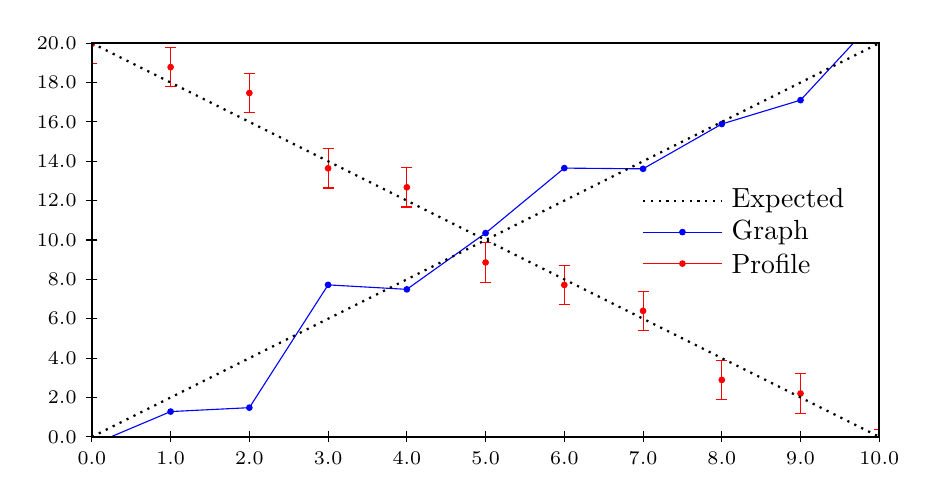
\begin{tikzpicture}
\draw[thick] (0,0) rectangle (10,5);
\begin{scope}
\clip (0,0) rectangle (10,5);
\draw[blue,fill=blue] (0.0,-0.10196566348827509) circle(1pt); 
\draw[blue,fill=blue] (1.0,0.32081350040858836) circle(1pt); 
\draw[blue,fill=blue] (2.0,0.37050159793480386) circle(1pt); 
\draw[blue,fill=blue] (3.0,1.929897193068983) circle(1pt); 
\draw[blue,fill=blue] (4.0,1.87296357584489) circle(1pt); 
\draw[blue,fill=blue] (5.0,2.587709257191488) circle(1pt); 
\draw[blue,fill=blue] (6.0,3.4128866484188434) circle(1pt); 
\draw[blue,fill=blue] (7.0,3.403718107491729) circle(1pt); 
\draw[blue,fill=blue] (8.0,3.972951194427708) circle(1pt); 
\draw[blue,fill=blue] (9.0,4.275955633054004) circle(1pt); 
\draw[blue,fill=blue] (10.0,5.354815652090555) circle(1pt); 
\draw[smooth,blue] (0.0,-0.10196566348827509) -- (1.0,0.32081350040858836);
\draw[smooth,blue] (1.0,0.32081350040858836) -- (2.0,0.37050159793480386);
\draw[smooth,blue] (2.0,0.37050159793480386) -- (3.0,1.929897193068983);
\draw[smooth,blue] (3.0,1.929897193068983) -- (4.0,1.87296357584489);
\draw[smooth,blue] (4.0,1.87296357584489) -- (5.0,2.587709257191488);
\draw[smooth,blue] (5.0,2.587709257191488) -- (6.0,3.4128866484188434);
\draw[smooth,blue] (6.0,3.4128866484188434) -- (7.0,3.403718107491729);
\draw[smooth,blue] (7.0,3.403718107491729) -- (8.0,3.972951194427708);
\draw[smooth,blue] (8.0,3.972951194427708) -- (9.0,4.275955633054004);
\draw[smooth,blue] (9.0,4.275955633054004) -- (10.0,5.354815652090555);
\draw[draw=red,fill=red] (0.0,4.740948517066136) -- (0.0,5.240948517066136);
\draw[draw=red,fill=red] (0.0,4.990948517066136) circle(1pt); 
\draw[draw=red,fill=red] (0.0cm -2pt,4.740948517066136) -- (0.0cm + 2pt,4.740948517066136);
\draw[draw=red,fill=red] (0.0cm -2pt,5.240948517066136) -- (0.0cm + 2pt,5.240948517066136);
\draw[draw=red,fill=red] (1.0,4.445123867089418) -- (1.0,4.945123867089418);
\draw[draw=red,fill=red] (1.0,4.695123867089418) circle(1pt); 
\draw[draw=red,fill=red] (1.0cm -2pt,4.445123867089418) -- (1.0cm + 2pt,4.445123867089418);
\draw[draw=red,fill=red] (1.0cm -2pt,4.945123867089418) -- (1.0cm + 2pt,4.945123867089418);
\draw[draw=red,fill=red] (2.0,4.1169150578887725) -- (2.0,4.6169150578887725);
\draw[draw=red,fill=red] (2.0,4.3669150578887725) circle(1pt); 
\draw[draw=red,fill=red] (2.0cm -2pt,4.1169150578887725) -- (2.0cm + 2pt,4.1169150578887725);
\draw[draw=red,fill=red] (2.0cm -2pt,4.6169150578887725) -- (2.0cm + 2pt,4.6169150578887725);
\draw[draw=red,fill=red] (3.0,3.160562822769026) -- (3.0,3.660562822769026);
\draw[draw=red,fill=red] (3.0,3.410562822769026) circle(1pt); 
\draw[draw=red,fill=red] (3.0cm -2pt,3.160562822769026) -- (3.0cm + 2pt,3.160562822769026);
\draw[draw=red,fill=red] (3.0cm -2pt,3.660562822769026) -- (3.0cm + 2pt,3.660562822769026);
\draw[draw=red,fill=red] (4.0,2.9194273909490707) -- (4.0,3.4194273909490707);
\draw[draw=red,fill=red] (4.0,3.1694273909490707) circle(1pt); 
\draw[draw=red,fill=red] (4.0cm -2pt,2.9194273909490707) -- (4.0cm + 2pt,2.9194273909490707);
\draw[draw=red,fill=red] (4.0cm -2pt,3.4194273909490707) -- (4.0cm + 2pt,3.4194273909490707);
\draw[draw=red,fill=red] (5.0,1.9644805550595663) -- (5.0,2.4644805550595663);
\draw[draw=red,fill=red] (5.0,2.2144805550595663) circle(1pt); 
\draw[draw=red,fill=red] (5.0cm -2pt,1.9644805550595663) -- (5.0cm + 2pt,1.9644805550595663);
\draw[draw=red,fill=red] (5.0cm -2pt,2.4644805550595663) -- (5.0cm + 2pt,2.4644805550595663);
\draw[draw=red,fill=red] (6.0,1.6789278084216874) -- (6.0,2.1789278084216877);
\draw[draw=red,fill=red] (6.0,1.9289278084216874) circle(1pt); 
\draw[draw=red,fill=red] (6.0cm -2pt,1.6789278084216874) -- (6.0cm + 2pt,1.6789278084216874);
\draw[draw=red,fill=red] (6.0cm -2pt,2.1789278084216877) -- (6.0cm + 2pt,2.1789278084216877);
\draw[draw=red,fill=red] (7.0,1.3499323250346875) -- (7.0,1.8499323250346875);
\draw[draw=red,fill=red] (7.0,1.5999323250346875) circle(1pt); 
\draw[draw=red,fill=red] (7.0cm -2pt,1.3499323250346875) -- (7.0cm + 2pt,1.3499323250346875);
\draw[draw=red,fill=red] (7.0cm -2pt,1.8499323250346875) -- (7.0cm + 2pt,1.8499323250346875);
\draw[draw=red,fill=red] (8.0,0.4732684396285174) -- (8.0,0.9732684396285174);
\draw[draw=red,fill=red] (8.0,0.7232684396285174) circle(1pt); 
\draw[draw=red,fill=red] (8.0cm -2pt,0.4732684396285174) -- (8.0cm + 2pt,0.4732684396285174);
\draw[draw=red,fill=red] (8.0cm -2pt,0.9732684396285174) -- (8.0cm + 2pt,0.9732684396285174);
\draw[draw=red,fill=red] (9.0,0.3004758507084322) -- (9.0,0.8004758507084322);
\draw[draw=red,fill=red] (9.0,0.5504758507084322) circle(1pt); 
\draw[draw=red,fill=red] (9.0cm -2pt,0.3004758507084322) -- (9.0cm + 2pt,0.3004758507084322);
\draw[draw=red,fill=red] (9.0cm -2pt,0.8004758507084322) -- (9.0cm + 2pt,0.8004758507084322);
\draw[draw=red,fill=red] (10.0,-0.40838146801071407) -- (10.0,0.09161853198928593);
\draw[draw=red,fill=red] (10.0,-0.15838146801071407) circle(1pt); 
\draw[draw=red,fill=red] (10.0cm -2pt,-0.40838146801071407) -- (10.0cm + 2pt,-0.40838146801071407);
\draw[draw=red,fill=red] (10.0cm -2pt,0.09161853198928593) -- (10.0cm + 2pt,0.09161853198928593);
\draw[thick,dotted] (7.0,3.0) -- (8.0,3.0);
\node[right,] at (8.0,3.0) {Expected};
\draw[blue,fill=blue] (7.5,2.6) circle(1pt); 
\draw[blue] (7.0,2.6) -- (8.0,2.6);
\node[right,] at (8.0,2.6) {Graph};
\draw[red,fill=red] (7.5,2.2) circle(1pt); 
\draw[red] (7.0,2.2) -- (8.0,2.2);
\node[right,] at (8.0,2.2) {Profile};
\end{scope}
\draw (0,0cm + 2pt) -- (0, 0cm -2pt) node[below] {\scriptsize{\num[round-mode=places,round-precision=1]{0}}};
\draw (1,0cm + 2pt) -- (1, 0cm -2pt) node[below] {\scriptsize{\num[round-mode=places,round-precision=1]{1}}};
\draw (2,0cm + 2pt) -- (2, 0cm -2pt) node[below] {\scriptsize{\num[round-mode=places,round-precision=1]{2}}};
\draw (3,0cm + 2pt) -- (3, 0cm -2pt) node[below] {\scriptsize{\num[round-mode=places,round-precision=1]{3}}};
\draw (4,0cm + 2pt) -- (4, 0cm -2pt) node[below] {\scriptsize{\num[round-mode=places,round-precision=1]{4}}};
\draw (5,0cm + 2pt) -- (5, 0cm -2pt) node[below] {\scriptsize{\num[round-mode=places,round-precision=1]{5}}};
\draw (6,0cm + 2pt) -- (6, 0cm -2pt) node[below] {\scriptsize{\num[round-mode=places,round-precision=1]{6}}};
\draw (7,0cm + 2pt) -- (7, 0cm -2pt) node[below] {\scriptsize{\num[round-mode=places,round-precision=1]{7}}};
\draw (8,0cm + 2pt) -- (8, 0cm -2pt) node[below] {\scriptsize{\num[round-mode=places,round-precision=1]{8}}};
\draw (9,0cm + 2pt) -- (9, 0cm -2pt) node[below] {\scriptsize{\num[round-mode=places,round-precision=1]{9}}};
\draw (10,0cm + 2pt) -- (10, 0cm -2pt) node[below] {\scriptsize{\num[round-mode=places,round-precision=1]{10}}};
\draw (0cm + 2pt,0.    ) -- (0cm-2pt,0.    ) node[left] {\scriptsize{\num[round-mode=places,round-precision=1]{0}}};
\draw (0cm + 2pt,0.5    ) -- (0cm-2pt,0.5    ) node[left] {\scriptsize{\num[round-mode=places,round-precision=1]{2}}};
\draw (0cm + 2pt,1.    ) -- (0cm-2pt,1.    ) node[left] {\scriptsize{\num[round-mode=places,round-precision=1]{4}}};
\draw (0cm + 2pt,1.5    ) -- (0cm-2pt,1.5    ) node[left] {\scriptsize{\num[round-mode=places,round-precision=1]{6}}};
\draw (0cm + 2pt,2.    ) -- (0cm-2pt,2.    ) node[left] {\scriptsize{\num[round-mode=places,round-precision=1]{8}}};
\draw (0cm + 2pt,2.5    ) -- (0cm-2pt,2.5    ) node[left] {\scriptsize{\num[round-mode=places,round-precision=1]{10}}};
\draw (0cm + 2pt,3.    ) -- (0cm-2pt,3.    ) node[left] {\scriptsize{\num[round-mode=places,round-precision=1]{12}}};
\draw (0cm + 2pt,3.5    ) -- (0cm-2pt,3.5    ) node[left] {\scriptsize{\num[round-mode=places,round-precision=1]{14}}};
\draw (0cm + 2pt,4.    ) -- (0cm-2pt,4.    ) node[left] {\scriptsize{\num[round-mode=places,round-precision=1]{16}}};
\draw (0cm + 2pt,4.5    ) -- (0cm-2pt,4.5    ) node[left] {\scriptsize{\num[round-mode=places,round-precision=1]{18}}};
\draw (0cm + 2pt,5.    ) -- (0cm-2pt,5.    ) node[left] {\scriptsize{\num[round-mode=places,round-precision=1]{20}}};
\draw[thick,dotted] (0.0,0.0) -- (10.0,5.0);
\draw[thick,dotted] (0.0,5.0) -- (10.0,0.0);
\draw[thick] (0,0) rectangle (10,5);
\end{tikzpicture}
%%% Local Variables: 
%%% mode: latex 
%%% TeX-master: "master" 
%%% End:


  \caption{Data points with and without errors}
\end{figure}

\begin{figure}[H]
  \centering
  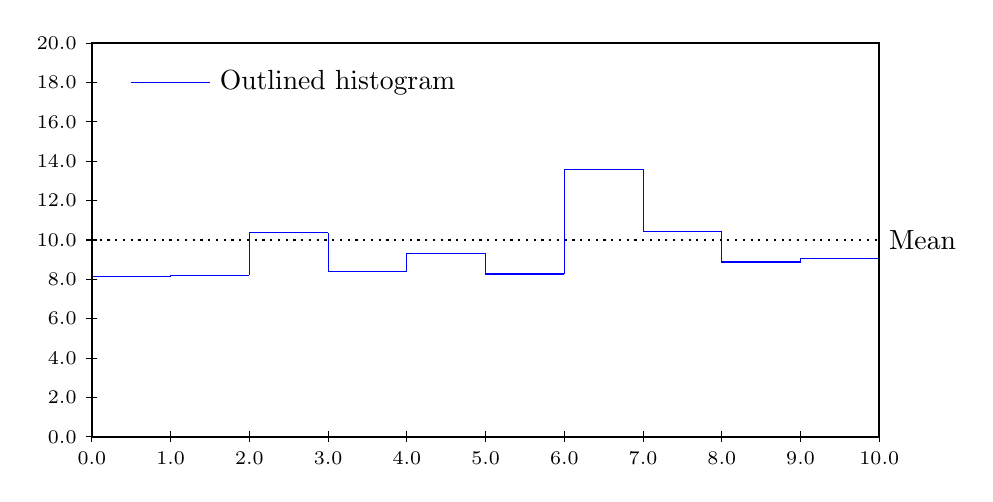
\begin{tikzpicture}
\begin{scope}[]
\clip (0,0) rectangle (10,5);
\begin{scope}[blue]
\draw[] (0.0,2.040753989729346) -- (1.0,2.040753989729346);
\draw (1.0,2.040753989729346) -- (1.0,2.0520371396851527) -- (2.0,2.0520371396851527);
\draw (2.0,2.0520371396851527) -- (2.0,2.589490136587087) -- (3.0,2.589490136587087);
\draw (3.0,2.589490136587087) -- (3.0,2.10531930397396) -- (4.0,2.10531930397396);
\draw (4.0,2.10531930397396) -- (4.0,2.328047479221825) -- (5.0,2.328047479221825);
\draw (5.0,2.328047479221825) -- (5.0,2.067390163042384) -- (6.0,2.067390163042384);
\draw (6.0,2.067390163042384) -- (6.0,3.3961419895360887) -- (7.0,3.3961419895360887);
\draw (7.0,3.3961419895360887) -- (7.0,2.6085288458106475) -- (8.0,2.6085288458106475);
\draw (8.0,2.6085288458106475) -- (8.0,2.2210174657245827) -- (9.0,2.2210174657245827);
\draw (9.0,2.2210174657245827) -- (9.0,2.2670683657782047) -- (10.0,2.2670683657782047);
\end{scope}
\end{scope}
\draw (0,0cm + 2pt) -- (0, 0cm -2pt) node[below] {\scriptsize{\num[round-mode=places,round-precision=1]{0}}};
\draw (1,0cm + 2pt) -- (1, 0cm -2pt) node[below] {\scriptsize{\num[round-mode=places,round-precision=1]{1}}};
\draw (2,0cm + 2pt) -- (2, 0cm -2pt) node[below] {\scriptsize{\num[round-mode=places,round-precision=1]{2}}};
\draw (3,0cm + 2pt) -- (3, 0cm -2pt) node[below] {\scriptsize{\num[round-mode=places,round-precision=1]{3}}};
\draw (4,0cm + 2pt) -- (4, 0cm -2pt) node[below] {\scriptsize{\num[round-mode=places,round-precision=1]{4}}};
\draw (5,0cm + 2pt) -- (5, 0cm -2pt) node[below] {\scriptsize{\num[round-mode=places,round-precision=1]{5}}};
\draw (6,0cm + 2pt) -- (6, 0cm -2pt) node[below] {\scriptsize{\num[round-mode=places,round-precision=1]{6}}};
\draw (7,0cm + 2pt) -- (7, 0cm -2pt) node[below] {\scriptsize{\num[round-mode=places,round-precision=1]{7}}};
\draw (8,0cm + 2pt) -- (8, 0cm -2pt) node[below] {\scriptsize{\num[round-mode=places,round-precision=1]{8}}};
\draw (9,0cm + 2pt) -- (9, 0cm -2pt) node[below] {\scriptsize{\num[round-mode=places,round-precision=1]{9}}};
\draw (10,0cm + 2pt) -- (10, 0cm -2pt) node[below] {\scriptsize{\num[round-mode=places,round-precision=1]{10}}};
\draw (0cm + 2pt,0.    ) -- (0cm-2pt,0.    ) node[left] {\scriptsize{\num[round-mode=places,round-precision=1]{0}}};
\draw (0cm + 2pt,0.5    ) -- (0cm-2pt,0.5    ) node[left] {\scriptsize{\num[round-mode=places,round-precision=1]{2}}};
\draw (0cm + 2pt,1.    ) -- (0cm-2pt,1.    ) node[left] {\scriptsize{\num[round-mode=places,round-precision=1]{4}}};
\draw (0cm + 2pt,1.5    ) -- (0cm-2pt,1.5    ) node[left] {\scriptsize{\num[round-mode=places,round-precision=1]{6}}};
\draw (0cm + 2pt,2.    ) -- (0cm-2pt,2.    ) node[left] {\scriptsize{\num[round-mode=places,round-precision=1]{8}}};
\draw (0cm + 2pt,2.5    ) -- (0cm-2pt,2.5    ) node[left] {\scriptsize{\num[round-mode=places,round-precision=1]{10}}};
\draw (0cm + 2pt,3.    ) -- (0cm-2pt,3.    ) node[left] {\scriptsize{\num[round-mode=places,round-precision=1]{12}}};
\draw (0cm + 2pt,3.5    ) -- (0cm-2pt,3.5    ) node[left] {\scriptsize{\num[round-mode=places,round-precision=1]{14}}};
\draw (0cm + 2pt,4.    ) -- (0cm-2pt,4.    ) node[left] {\scriptsize{\num[round-mode=places,round-precision=1]{16}}};
\draw (0cm + 2pt,4.5    ) -- (0cm-2pt,4.5    ) node[left] {\scriptsize{\num[round-mode=places,round-precision=1]{18}}};
\draw (0cm + 2pt,5.    ) -- (0cm-2pt,5.    ) node[left] {\scriptsize{\num[round-mode=places,round-precision=1]{20}}};
\draw[thick] (0,0) rectangle (10,5);
\draw[thick,dotted] (0.0,2.5) -- (10.0,2.5);
\node[right] at (10.0,2.5) {Mean};
\draw[blue] (0.5,4.5) -- (1.5,4.5);
\node[right,] at (1.5,4.5) {Outlined histogram};
\end{tikzpicture}
%%% Local Variables: 
%%% mode: latex 
%%% TeX-master: "master" 
%%% End:


  \caption{Basic histogram}
\end{figure}

\begin{figure}[H]
  \centering
  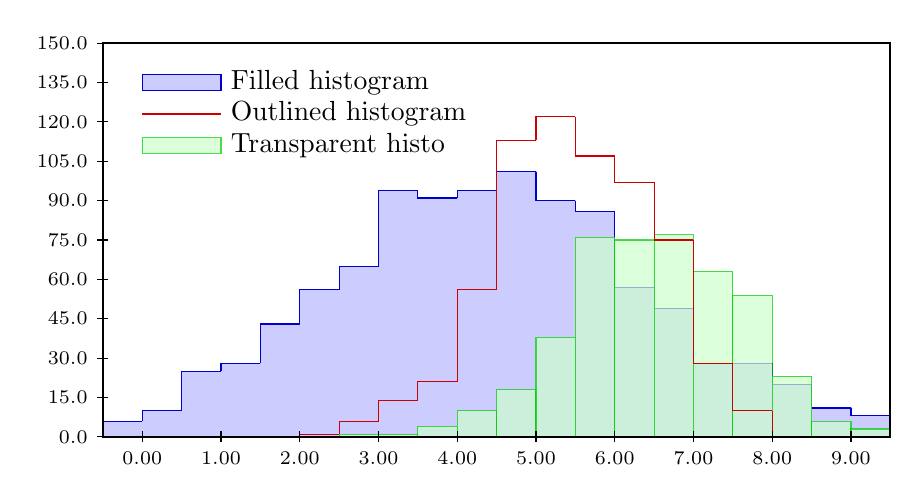
\begin{tikzpicture}
\begin{scope}[]
\clip (0,0) rectangle (10,5);
\begin{scope}[draw=blue!20,fill=blue!20]
\filldraw[] (0.0,0.0) -- (0.0,0.2) -- (0.5,0.2) -- (0.5,0.0);
\filldraw[] (0.5,0.0) -- (0.5,0.33333334) -- (1.0,0.33333334) -- (1.0,0.0);
\filldraw[] (1.0,0.0) -- (1.0,0.8333333) -- (1.5,0.8333333) -- (1.5,0.0);
\filldraw[] (1.5,0.0) -- (1.5,0.93333334) -- (2.0,0.93333334) -- (2.0,0.0);
\filldraw[] (2.0,0.0) -- (2.0,1.4333333) -- (2.5,1.4333333) -- (2.5,0.0);
\filldraw[] (2.5,0.0) -- (2.5,1.8666667) -- (3.0,1.8666667) -- (3.0,0.0);
\filldraw[] (3.0,0.0) -- (3.0,2.1666667) -- (3.5,2.1666667) -- (3.5,0.0);
\filldraw[] (3.5,0.0) -- (3.5,3.1333334) -- (4.0,3.1333334) -- (4.0,0.0);
\filldraw[] (4.0,0.0) -- (4.0,3.0333333) -- (4.5,3.0333333) -- (4.5,0.0);
\filldraw[] (4.5,0.0) -- (4.5,3.1333334) -- (5.0,3.1333334) -- (5.0,0.0);
\filldraw[] (5.0,0.0) -- (5.0,3.3666666) -- (5.5,3.3666666) -- (5.5,0.0);
\filldraw[] (5.5,0.0) -- (5.5,3.0) -- (6.0,3.0) -- (6.0,0.0);
\filldraw[] (6.0,0.0) -- (6.0,2.8666666) -- (6.5,2.8666666) -- (6.5,0.0);
\filldraw[] (6.5,0.0) -- (6.5,1.9) -- (7.0,1.9) -- (7.0,0.0);
\filldraw[] (7.0,0.0) -- (7.0,1.6333333) -- (7.5,1.6333333) -- (7.5,0.0);
\filldraw[] (7.5,0.0) -- (7.5,0.93333334) -- (8.0,0.93333334) -- (8.0,0.0);
\filldraw[] (8.0,0.0) -- (8.0,0.93333334) -- (8.5,0.93333334) -- (8.5,0.0);
\filldraw[] (8.5,0.0) -- (8.5,0.6666667) -- (9.0,0.6666667) -- (9.0,0.0);
\filldraw[] (9.0,0.0) -- (9.0,0.36666667) -- (9.5,0.36666667) -- (9.5,0.0);
\filldraw[] (9.5,0.0) -- (9.5,0.26666668) -- (10.0,0.26666668) -- (10.0,0.0);
\end{scope}
\begin{scope}[blue!80!black]
\draw[] (0.0,0.2) -- (0.5,0.2);
\draw (0.5,0.2) -- (0.5,0.33333334) -- (1.0,0.33333334);
\draw (1.0,0.33333334) -- (1.0,0.8333333) -- (1.5,0.8333333);
\draw (1.5,0.8333333) -- (1.5,0.93333334) -- (2.0,0.93333334);
\draw (2.0,0.93333334) -- (2.0,1.4333333) -- (2.5,1.4333333);
\draw (2.5,1.4333333) -- (2.5,1.8666667) -- (3.0,1.8666667);
\draw (3.0,1.8666667) -- (3.0,2.1666667) -- (3.5,2.1666667);
\draw (3.5,2.1666667) -- (3.5,3.1333334) -- (4.0,3.1333334);
\draw (4.0,3.1333334) -- (4.0,3.0333333) -- (4.5,3.0333333);
\draw (4.5,3.0333333) -- (4.5,3.1333334) -- (5.0,3.1333334);
\draw (5.0,3.1333334) -- (5.0,3.3666666) -- (5.5,3.3666666);
\draw (5.5,3.3666666) -- (5.5,3.0) -- (6.0,3.0);
\draw (6.0,3.0) -- (6.0,2.8666666) -- (6.5,2.8666666);
\draw (6.5,2.8666666) -- (6.5,1.9) -- (7.0,1.9);
\draw (7.0,1.9) -- (7.0,1.6333333) -- (7.5,1.6333333);
\draw (7.5,1.6333333) -- (7.5,0.93333334) -- (8.0,0.93333334);
\draw (8.0,0.93333334) -- (8.0,0.93333334) -- (8.5,0.93333334);
\draw (8.5,0.93333334) -- (8.5,0.6666667) -- (9.0,0.6666667);
\draw (9.0,0.6666667) -- (9.0,0.36666667) -- (9.5,0.36666667);
\draw (9.5,0.36666667) -- (9.5,0.26666668) -- (10.0,0.26666668);
\end{scope}
\begin{scope}[opacity=0.7,draw=green!80!black,fill=green!20]
\filldraw[] (0.0,0.0) -- (0.0,0.0) -- (0.5,0.0) -- (0.5,0.0);
\filldraw[] (0.5,0.0) -- (0.5,0.0) -- (1.0,0.0) -- (1.0,0.0);
\filldraw[] (1.0,0.0) -- (1.0,0.0) -- (1.5,0.0) -- (1.5,0.0);
\filldraw[] (1.5,0.0) -- (1.5,0.0) -- (2.0,0.0) -- (2.0,0.0);
\filldraw[] (2.0,0.0) -- (2.0,0.0) -- (2.5,0.0) -- (2.5,0.0);
\filldraw[] (2.5,0.0) -- (2.5,0.0) -- (3.0,0.0) -- (3.0,0.0);
\filldraw[] (3.0,0.0) -- (3.0,0.033333335) -- (3.5,0.033333335) -- (3.5,0.0);
\filldraw[] (3.5,0.0) -- (3.5,0.033333335) -- (4.0,0.033333335) -- (4.0,0.0);
\filldraw[] (4.0,0.0) -- (4.0,0.13333334) -- (4.5,0.13333334) -- (4.5,0.0);
\filldraw[] (4.5,0.0) -- (4.5,0.33333334) -- (5.0,0.33333334) -- (5.0,0.0);
\filldraw[] (5.0,0.0) -- (5.0,0.6) -- (5.5,0.6) -- (5.5,0.0);
\filldraw[] (5.5,0.0) -- (5.5,1.2666667) -- (6.0,1.2666667) -- (6.0,0.0);
\filldraw[] (6.0,0.0) -- (6.0,2.5333333) -- (6.5,2.5333333) -- (6.5,0.0);
\filldraw[] (6.5,0.0) -- (6.5,2.5) -- (7.0,2.5) -- (7.0,0.0);
\filldraw[] (7.0,0.0) -- (7.0,2.5666666) -- (7.5,2.5666666) -- (7.5,0.0);
\filldraw[] (7.5,0.0) -- (7.5,2.1) -- (8.0,2.1) -- (8.0,0.0);
\filldraw[] (8.0,0.0) -- (8.0,1.8) -- (8.5,1.8) -- (8.5,0.0);
\filldraw[] (8.5,0.0) -- (8.5,0.76666665) -- (9.0,0.76666665) -- (9.0,0.0);
\filldraw[] (9.0,0.0) -- (9.0,0.2) -- (9.5,0.2) -- (9.5,0.0);
\filldraw[] (9.5,0.0) -- (9.5,0.1) -- (10.0,0.1) -- (10.0,0.0);
\end{scope}
\begin{scope}[red!80!black]
\draw[] (0.0,0.0) -- (0.5,0.0);
\draw (0.5,0.0) -- (0.5,0.0) -- (1.0,0.0);
\draw (1.0,0.0) -- (1.0,0.0) -- (1.5,0.0);
\draw (1.5,0.0) -- (1.5,0.0) -- (2.0,0.0);
\draw (2.0,0.0) -- (2.0,0.0) -- (2.5,0.0);
\draw (2.5,0.0) -- (2.5,0.033333335) -- (3.0,0.033333335);
\draw (3.0,0.033333335) -- (3.0,0.2) -- (3.5,0.2);
\draw (3.5,0.2) -- (3.5,0.46666667) -- (4.0,0.46666667);
\draw (4.0,0.46666667) -- (4.0,0.7) -- (4.5,0.7);
\draw (4.5,0.7) -- (4.5,1.8666667) -- (5.0,1.8666667);
\draw (5.0,1.8666667) -- (5.0,3.7666667) -- (5.5,3.7666667);
\draw (5.5,3.7666667) -- (5.5,4.0666666) -- (6.0,4.0666666);
\draw (6.0,4.0666666) -- (6.0,3.5666666) -- (6.5,3.5666666);
\draw (6.5,3.5666666) -- (6.5,3.2333333) -- (7.0,3.2333333);
\draw (7.0,3.2333333) -- (7.0,2.5) -- (7.5,2.5);
\draw (7.5,2.5) -- (7.5,0.93333334) -- (8.0,0.93333334);
\draw (8.0,0.93333334) -- (8.0,0.33333334) -- (8.5,0.33333334);
\draw (8.5,0.33333334) -- (8.5,0.0) -- (9.0,0.0);
\draw (9.0,0.0) -- (9.0,0.0) -- (9.5,0.0);
\draw (9.5,0.0) -- (9.5,0.0) -- (10.0,0.0);
\end{scope}
\end{scope}
\draw (0.5,0cm + 2pt) -- (0.5, 0cm -2pt) node[below] {\scriptsize{\num[round-mode=places,round-precision=2]{0}}};
\draw (1.5,0cm + 2pt) -- (1.5, 0cm -2pt) node[below] {\scriptsize{\num[round-mode=places,round-precision=2]{1}}};
\draw (2.5,0cm + 2pt) -- (2.5, 0cm -2pt) node[below] {\scriptsize{\num[round-mode=places,round-precision=2]{2}}};
\draw (3.5,0cm + 2pt) -- (3.5, 0cm -2pt) node[below] {\scriptsize{\num[round-mode=places,round-precision=2]{3}}};
\draw (4.5,0cm + 2pt) -- (4.5, 0cm -2pt) node[below] {\scriptsize{\num[round-mode=places,round-precision=2]{4}}};
\draw (5.5,0cm + 2pt) -- (5.5, 0cm -2pt) node[below] {\scriptsize{\num[round-mode=places,round-precision=2]{5}}};
\draw (6.5,0cm + 2pt) -- (6.5, 0cm -2pt) node[below] {\scriptsize{\num[round-mode=places,round-precision=2]{6}}};
\draw (7.5,0cm + 2pt) -- (7.5, 0cm -2pt) node[below] {\scriptsize{\num[round-mode=places,round-precision=2]{7}}};
\draw (8.5,0cm + 2pt) -- (8.5, 0cm -2pt) node[below] {\scriptsize{\num[round-mode=places,round-precision=2]{8}}};
\draw (9.5,0cm + 2pt) -- (9.5, 0cm -2pt) node[below] {\scriptsize{\num[round-mode=places,round-precision=2]{9}}};
\draw (0cm + 2pt,0.    ) -- (0cm-2pt,0.    ) node[left] {\scriptsize{\num[round-mode=places,round-precision=1]{0}}};
\draw (0cm + 2pt,0.5    ) -- (0cm-2pt,0.5    ) node[left] {\scriptsize{\num[round-mode=places,round-precision=1]{15}}};
\draw (0cm + 2pt,1.    ) -- (0cm-2pt,1.    ) node[left] {\scriptsize{\num[round-mode=places,round-precision=1]{30}}};
\draw (0cm + 2pt,1.5    ) -- (0cm-2pt,1.5    ) node[left] {\scriptsize{\num[round-mode=places,round-precision=1]{45}}};
\draw (0cm + 2pt,2.    ) -- (0cm-2pt,2.    ) node[left] {\scriptsize{\num[round-mode=places,round-precision=1]{60}}};
\draw (0cm + 2pt,2.5    ) -- (0cm-2pt,2.5    ) node[left] {\scriptsize{\num[round-mode=places,round-precision=1]{75}}};
\draw (0cm + 2pt,3.    ) -- (0cm-2pt,3.    ) node[left] {\scriptsize{\num[round-mode=places,round-precision=1]{90}}};
\draw (0cm + 2pt,3.5    ) -- (0cm-2pt,3.5    ) node[left] {\scriptsize{\num[round-mode=places,round-precision=1]{105}}};
\draw (0cm + 2pt,4.    ) -- (0cm-2pt,4.    ) node[left] {\scriptsize{\num[round-mode=places,round-precision=1]{120}}};
\draw (0cm + 2pt,4.5    ) -- (0cm-2pt,4.5    ) node[left] {\scriptsize{\num[round-mode=places,round-precision=1]{135}}};
\draw (0cm + 2pt,5.    ) -- (0cm-2pt,5.    ) node[left] {\scriptsize{\num[round-mode=places,round-precision=1]{150}}};
\draw[thick] (0,0) rectangle (10,5);
\draw[draw=blue!20,fill=blue!20] (0.5,4.4) rectangle (1.5,4.6);
\draw[blue!80!black] (0.5,4.4) rectangle (1.5,4.6);
\node[right,] at (1.5,4.5) {Filled histogram};
\draw[red!80!black] (0.5,4.1) -- (1.5,4.1);
\node[right,] at (1.5,4.1) {Outlined histogram};
\draw[opacity=0.7,draw=green!80!black,fill=green!20] (0.5,3.6000001) rectangle (1.5,3.8);
\node[right,] at (1.5,3.7) {Transparent histo};
\end{tikzpicture}
%%% Local Variables: 
%%% mode: latex 
%%% TeX-master: "master" 
%%% End:


  \caption{Two histograms in the same figure}
\end{figure}

\section{Fitting with Levenberg marquart algorithm}
\label{sec:LMA}

\begin{figure}[H]
  \centering
  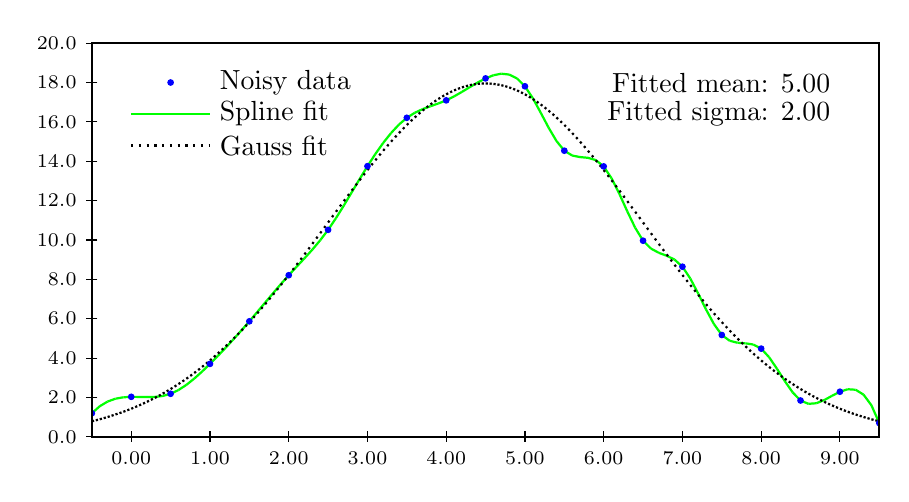
\begin{tikzpicture}
\begin{scope}[]
\clip (0,0) rectangle (10,5);
\begin{scope}[green,thick]
\draw[] (0.0,0.2998554191980206) -- (0.1,0.3886769723521621);
\draw[] (0.1,0.3886769723521621) -- (0.2,0.4483013692841718);
\draw[] (0.2,0.4483013692841718) -- (0.3,0.48433430438467895);
\draw[] (0.3,0.48433430438467895) -- (0.4,0.5023814720443124);
\draw[] (0.4,0.5023814720443124) -- (0.5,0.508048566653701);
\draw[] (0.5,0.508048566653701) -- (0.6,0.506941282603474);
\draw[] (0.6,0.506941282603474) -- (0.7,0.5046653142842601);
\draw[] (0.7,0.5046653142842601) -- (0.8,0.5068263560866882);
\draw[] (0.8,0.5068263560866882) -- (0.9,0.5190301024013876);
\draw[] (0.9,0.5190301024013876) -- (1.0,0.5468822476189868);
\draw[] (1.0,0.5468822476189868) -- (1.1,0.5944637212948228);
\draw[] (1.1,0.5944637212948228) -- (1.2,0.6597563936430622);
\draw[] (1.2,0.6597563936430622) -- (1.3,0.7392173700425795);
\draw[] (1.3,0.7392173700425795) -- (1.4,0.8293037558722491);
\draw[] (1.4,0.8293037558722491) -- (1.5,0.9264726565109458);
\draw[] (1.5,0.9264726565109458) -- (1.6,1.0277622403859983);
\draw[] (1.6,1.0277622403859983) -- (1.7,1.1325349281185535);
\draw[] (1.7,1.1325349281185535) -- (1.8,1.2407342033782138);
\draw[] (1.8,1.2407342033782138) -- (1.9,1.3523035498345806);
\draw[] (1.9,1.3523035498345806) -- (2.0,1.4671864511572559);
\draw[] (2.0,1.4671864511572559) -- (2.1,1.5850318885919035);
\draw[] (2.1,1.5850318885919035) -- (2.2,1.7043108336884367);
\draw[] (2.2,1.7043108336884367) -- (2.3,1.8231997555728292);
\draw[] (2.3,1.8231997555728292) -- (2.4,1.9398751233710578);
\draw[] (2.4,1.9398751233710578) -- (2.5,2.052513406209097);
\draw[] (2.5,2.052513406209097) -- (2.6,2.1603895447518);
\draw[] (2.6,2.1603895447518) -- (2.7,2.2671723658195386);
\draw[] (2.7,2.2671723658195386) -- (2.8,2.37762916777156);
\draw[] (2.8,2.37762916777156) -- (2.9,2.496527248967116);
\draw[] (2.9,2.496527248967116) -- (3.0,2.6286339077654537);
\draw[] (3.0,2.6286339077654537) -- (3.1,2.7769838678261562);
\draw[] (3.1,2.7769838678261562) -- (3.2,2.937681554010137);
\draw[] (3.2,2.937681554010137) -- (3.3,3.1050988164786424);
\draw[] (3.3,3.1050988164786424) -- (3.4,3.2736075053929206);
\draw[] (3.4,3.2736075053929206) -- (3.5,3.437579470914217);
\draw[] (3.5,3.437579470914217) -- (3.6,3.5918608991118726);
\draw[] (3.6,3.5918608991118726) -- (3.7,3.7331953196876033);
\draw[] (3.7,3.7331953196876033) -- (3.8,3.8588005982512175);
\draw[] (3.8,3.8588005982512175) -- (3.9,3.965894600412527);
\draw[] (3.9,3.965894600412527) -- (4.0,4.051695191781341);
\draw[] (4.0,4.051695191781341) -- (4.1,4.115095756069382);
\draw[] (4.1,4.115095756069382) -- (4.2,4.161691749396038);
\draw[] (4.2,4.161691749396038) -- (4.3,4.198754145982606);
\draw[] (4.3,4.198754145982606) -- (4.4,4.233553920050386);
\draw[] (4.4,4.233553920050386) -- (4.5,4.273362045820676);
\draw[] (4.5,4.273362045820676) -- (4.6,4.3234520701688135);
\draw[] (4.6,4.3234520701688135) -- (4.7,4.381107830586282);
\draw[] (4.7,4.381107830586282) -- (4.8,4.441615737218599);
\draw[] (4.8,4.441615737218599) -- (4.9,4.500262200211288);
\draw[] (4.9,4.500262200211288) -- (5.0,4.552333629709862);
\draw[] (5.0,4.552333629709862) -- (5.1,4.59233776594064);
\draw[] (5.1,4.59233776594064) -- (5.2,4.611667669453102);
\draw[] (5.2,4.611667669453102) -- (5.3,4.600937730877521);
\draw[] (5.3,4.600937730877521) -- (5.4,4.550762340844171);
\draw[] (5.4,4.550762340844171) -- (5.5,4.45175588998333);
\draw[] (5.5,4.45175588998333) -- (5.6,4.300437582389341);
\draw[] (5.6,4.300437582389341) -- (5.7,4.116945876012824);
\draw[] (5.7,4.116945876012824) -- (5.8,3.9273240422684816);
\draw[] (5.8,3.9273240422684816) -- (5.9,3.7576153525710008);
\draw[] (5.9,3.7576153525710008) -- (6.0,3.633863078335081);
\draw[] (6.0,3.633863078335081) -- (6.1,3.572659679395789);
\draw[] (6.1,3.572659679395789) -- (6.2,3.5527943692696895);
\draw[] (6.2,3.5527943692696895) -- (6.3,3.543605549893723);
\draw[] (6.3,3.543605549893723) -- (6.4,3.5144316232048283);
\draw[] (6.4,3.5144316232048283) -- (6.5,3.4346109911399463);
\draw[] (6.5,3.4346109911399463) -- (6.6,3.2837879915385906);
\draw[] (6.6,3.2837879915385906) -- (6.7,3.082830705850571);
\draw[] (6.7,3.082830705850571) -- (6.8,2.862913151428279);
\draw[] (6.8,2.862913151428279) -- (6.9,2.655209345624097);
\draw[] (6.9,2.655209345624097) -- (7.0,2.490893305790417);
\draw[] (7.0,2.490893305790417) -- (7.1,2.3911350529230266);
\draw[] (7.1,2.3911350529230266) -- (7.2,2.337088622591336);
\draw[] (7.2,2.337088622591336) -- (7.3,2.299904054008158);
\draw[] (7.3,2.299904054008158) -- (7.4,2.2507313863863057);
\draw[] (7.4,2.2507313863863057) -- (7.5,2.1607206589385934);
\draw[] (7.5,2.1607206589385934) -- (7.6,2.0106625992444567);
\draw[] (7.6,2.0106625992444567) -- (7.7,1.8199106883498228);
\draw[] (7.7,1.8199106883498228) -- (7.8,1.6174590956672459);
\draw[] (7.8,1.6174590956672459) -- (7.9,1.4323019906092747);
\draw[] (7.9,1.4323019906092747) -- (8.0,1.293433542588464);
\draw[] (8.0,1.293433542588464) -- (8.1,1.220344741560056);
\draw[] (8.1,1.220344741560056) -- (8.2,1.1945138596500657);
\draw[] (8.2,1.1945138596500657) -- (8.3,1.1879159895272018);
\draw[] (8.3,1.1879159895272018) -- (8.4,1.172526223860172);
\draw[] (8.4,1.172526223860172) -- (8.5,1.1203196553176844);
\draw[] (8.5,1.1203196553176844) -- (8.6,1.012354246334453);
\draw[] (8.6,1.012354246334453) -- (8.7,0.8660194384092178);
\draw[] (8.7,0.8660194384092178) -- (8.8,0.707787542806721);
\draw[] (8.8,0.707787542806721) -- (8.9,0.5641308707917143);
\draw[] (8.9,0.5641308707917143) -- (9.0,0.46152173362894033);
\draw[] (9.0,0.46152173362894033) -- (9.1,0.41909065427502007);
\draw[] (9.1,0.41909065427502007) -- (9.2,0.4266010024540752);
\draw[] (9.2,0.4266010024540752) -- (9.3,0.46647435958210365);
\draw[] (9.3,0.46647435958210365) -- (9.4,0.5211323070751007);
\draw[] (9.4,0.5211323070751007) -- (9.5,0.5729964263490639);
\draw[] (9.5,0.5729964263490639) -- (9.6,0.6044882988199899);
\draw[] (9.6,0.6044882988199899) -- (9.7,0.5980295059038759);
\draw[] (9.7,0.5980295059038759) -- (9.8,0.5360416290167176);
\draw[] (9.8,0.5360416290167176) -- (9.9,0.4009462495745133);
\draw[] (9.9,0.4009462495745133) -- (10.0,0.1751649489932598);
\end{scope}
\begin{scope}[dotted, thick]
\draw[] (0.0,0.19719338055255084) -- (0.05,0.20984567391293701);
\draw[] (0.05,0.20984567391293701) -- (0.1,0.2231702369075935);
\draw[] (0.1,0.2231702369075935) -- (0.15,0.23719257748861314);
\draw[] (0.15,0.23719257748861314) -- (0.2,0.25193846581686985);
\draw[] (0.2,0.25193846581686985) -- (0.25,0.26743388433641285);
\draw[] (0.25,0.26743388433641285) -- (0.3,0.2837049740458145);
\draw[] (0.3,0.2837049740458145) -- (0.35,0.3007779769376655);
\draw[] (0.35,0.3007779769376655) -- (0.4,0.3186791745928813);
\draw[] (0.4,0.3186791745928813) -- (0.45,0.33743482293299765);
\draw[] (0.45,0.33743482293299765) -- (0.5,0.3570710831511164);
\draw[] (0.5,0.3570710831511164) -- (0.55,0.37761394886060007);
\draw[] (0.55,0.37761394886060007) -- (0.6,0.3990891695199511);
\draw[] (0.6,0.3990891695199511) -- (0.65,0.42152217021247246);
\draw[] (0.65,0.42152217021247246) -- (0.7,0.444937967880252);
\draw[] (0.7,0.444937967880252) -- (0.75,0.46936108413364097);
\draw[] (0.75,0.46936108413364097) -- (0.8,0.49481545477963207);
\draw[] (0.8,0.49481545477963207) -- (0.85,0.5213243362352994);
\draw[] (0.85,0.5213243362352994) -- (0.9,0.5489102090156216);
\draw[] (0.9,0.5489102090156216) -- (0.95,0.5775946785084662);
\draw[] (0.95,0.5775946785084662) -- (1.0,0.60739837327317);
\draw[] (1.0,0.60739837327317) -- (1.05,0.6383408411228194);
\draw[] (1.05,0.6383408411228194) -- (1.1,0.6704404432739747);
\draw[] (1.1,0.6704404432739747) -- (1.15,0.7037142468709632);
\draw[] (1.15,0.7037142468709632) -- (1.2,0.738177916214895);
\draw[] (1.2,0.738177916214895) -- (1.25,0.7738456030500619);
\draw[] (1.25,0.7738456030500619) -- (1.3,0.8107298362822254);
\draw[] (1.3,0.8107298362822254) -- (1.35,0.8488414115242828);
\draw[] (1.35,0.8488414115242828) -- (1.4,0.8881892808848224);
\draw[] (1.4,0.8881892808848224) -- (1.45,0.9287804434339139);
\draw[] (1.45,0.9287804434339139) -- (1.5,0.9706198367980078);
\draw[] (1.5,0.9706198367980078) -- (1.55,1.0137102303518524);
\draw[] (1.55,1.0137102303518524) -- (1.6,1.0580521204897222);
\draw[] (1.6,1.0580521204897222) -- (1.65,1.1036436284708402);
\draw[] (1.65,1.1036436284708402) -- (1.7,1.1504804013444883);
\draw[] (1.7,1.1504804013444883) -- (1.75,1.1985555164688135);
\draw[] (1.75,1.1985555164688135) -- (1.8,1.2478593901436028);
\draw[] (1.8,1.2478593901436028) -- (1.85,1.2983796908811616);
\draw[] (1.85,1.2983796908811616) -- (1.9,1.350101257840809);
\draw[] (1.9,1.350101257840809) -- (1.95,1.4030060249512366);
\draw[] (1.95,1.4030060249512366) -- (2.0,1.4570729512409966);
\draw[] (2.0,1.4570729512409966) -- (2.05,1.5122779578906014);
\draw[] (2.05,1.5122779578906014) -- (2.1,1.5685938725100126);
\draw[] (2.1,1.5685938725100126) -- (2.15,1.6259903811327017);
\draw[] (2.15,1.6259903811327017) -- (2.2,1.6844339884018351);
\draw[] (2.2,1.6844339884018351) -- (2.25,1.743887986405502);
\draw[] (2.25,1.743887986405502) -- (2.3,1.8043124325962971);
\draw[] (2.3,1.8043124325962971) -- (2.35,1.865664137205879);
\draw[] (2.35,1.865664137205879) -- (2.4,1.9278966605375325);
\draw[] (2.4,1.9278966605375325) -- (2.45,1.9909603204892214);
\draw[] (2.45,1.9909603204892214) -- (2.5,2.0548022106261956);
\draw[] (2.5,2.0548022106261956) -- (2.55,2.11936622908612);
\draw[] (2.55,2.11936622908612) -- (2.6,2.184593118560845);
\draw[] (2.6,2.184593118560845) -- (2.65,2.250420517557687);
\draw[] (2.65,2.250420517557687) -- (2.7,2.3167830230994166);
\draw[] (2.7,2.3167830230994166) -- (2.75,2.3836122649763207);
\draw[] (2.75,2.3836122649763207) -- (2.8,2.4508369916158963);
\draw[] (2.8,2.4508369916158963) -- (2.85,2.5183831675861494);
\draw[] (2.85,2.5183831675861494) -- (2.9,2.586174082697328);
\draw[] (2.9,2.586174082697328) -- (2.95,2.654130472614525);
\draw[] (2.95,2.654130472614525) -- (3.0,2.722170650840074);
\draw[] (3.0,2.722170650840074) -- (3.05,2.7902106518705065);
\draw[] (3.05,2.7902106518705065) -- (3.1,2.8581643852780934);
\draw[] (3.1,2.8581643852780934) -- (3.15,2.925943800412172);
\draw[] (3.15,2.925943800412172) -- (3.2,2.9934590613607153);
\draw[] (3.2,2.9934590613607153) -- (3.25,3.0606187317583413);
\draw[] (3.25,3.0606187317583413) -- (3.3,3.127329968973441);
\draw[] (3.3,3.127329968973441) -- (3.35,3.193498727154717);
\draw[] (3.35,3.193498727154717) -- (3.4,3.2590299685664195);
\draw[] (3.4,3.2590299685664195) -- (3.45,3.323827882592326);
\draw[] (3.45,3.323827882592326) -- (3.5,3.387796111741297);
\draw[] (3.5,3.387796111741297) -- (3.55,3.450837983942451);
\draw[] (3.55,3.450837983942451) -- (3.6,3.5128567503758203);
\draw[] (3.6,3.5128567503758203) -- (3.65,3.5737558280451784);
\draw[] (3.65,3.5737558280451784) -- (3.7,3.6334390462638013);
\draw[] (3.7,3.6334390462638013) -- (3.75,3.6918108961914897);
\draw[] (3.75,3.6918108961914897) -- (3.8,3.7487767825325204);
\draw[] (3.8,3.7487767825325204) -- (3.85,3.804243276479533);
\draw[] (3.85,3.804243276479533) -- (3.9,3.858118368967853);
\draw[] (3.9,3.858118368967853) -- (3.95,3.910311723288705);
\draw[] (3.95,3.910311723288705) -- (4.0,3.9607349260981626);
\draw[] (4.0,3.9607349260981626) -- (4.05,4.009301735851859);
\draw[] (4.05,4.009301735851859) -- (4.1,4.0559283276933416);
\draw[] (4.1,4.0559283276933416) -- (4.15,4.100533533826755);
\draw[] (4.15,4.100533533826755) -- (4.2,4.143039078412198);
\draw[] (4.2,4.143039078412198) -- (4.25,4.183369806034715);
\draw[] (4.25,4.183369806034715) -- (4.3,4.2214539028153695);
\draw[] (4.3,4.2214539028153695) -- (4.35,4.257223109255291);
\draw[] (4.35,4.257223109255291) -- (4.4,4.290612923930722);
\draw[] (4.4,4.290612923930722) -- (4.45,4.321562797189007);
\draw[] (4.45,4.321562797189007) -- (4.5,4.350016314031885);
\draw[] (4.5,4.350016314031885) -- (4.55,4.375921365413266);
\draw[] (4.55,4.375921365413266) -- (4.6,4.399230307223716);
\draw[] (4.6,4.399230307223716) -- (4.65,4.4199001062828565);
\draw[] (4.65,4.4199001062828565) -- (4.7,4.4378924727135916);
\draw[] (4.7,4.4378924727135916) -- (4.75,4.453173978128275);
\draw[] (4.75,4.453173978128275) -- (4.8,4.465716159116226);
\draw[] (4.8,4.465716159116226) -- (4.85,4.475495605584188);
\draw[] (4.85,4.475495605584188) -- (4.9,4.482494033565941);
\draw[] (4.9,4.482494033565941) -- (4.95,4.486698342184142);
\draw[] (4.95,4.486698342184142) -- (5.0,4.488100654515964);
\draw[] (5.0,4.488100654515964) -- (5.05,4.486698342184142);
\draw[] (5.05,4.486698342184142) -- (5.1,4.482494033565941);
\draw[] (5.1,4.482494033565941) -- (5.15,4.475495605584188);
\draw[] (5.15,4.475495605584188) -- (5.2,4.465716159116226);
\draw[] (5.2,4.465716159116226) -- (5.25,4.453173978128275);
\draw[] (5.25,4.453173978128275) -- (5.3,4.4378924727135916);
\draw[] (5.3,4.4378924727135916) -- (5.35,4.4199001062828565);
\draw[] (5.35,4.4199001062828565) -- (5.4,4.399230307223716);
\draw[] (5.4,4.399230307223716) -- (5.45,4.375921365413266);
\draw[] (5.45,4.375921365413266) -- (5.5,4.350016314031885);
\draw[] (5.5,4.350016314031885) -- (5.55,4.321562797189007);
\draw[] (5.55,4.321562797189007) -- (5.6,4.290612923930722);
\draw[] (5.6,4.290612923930722) -- (5.65,4.257223109255291);
\draw[] (5.65,4.257223109255291) -- (5.7,4.2214539028153695);
\draw[] (5.7,4.2214539028153695) -- (5.75,4.183369806034715);
\draw[] (5.75,4.183369806034715) -- (5.8,4.143039078412198);
\draw[] (5.8,4.143039078412198) -- (5.85,4.100533533826755);
\draw[] (5.85,4.100533533826755) -- (5.9,4.0559283276933416);
\draw[] (5.9,4.0559283276933416) -- (5.95,4.009301735851859);
\draw[] (5.95,4.009301735851859) -- (6.0,3.9607349260981626);
\draw[] (6.0,3.9607349260981626) -- (6.05,3.910311723288705);
\draw[] (6.05,3.910311723288705) -- (6.1,3.8581183689678533);
\draw[] (6.1,3.8581183689678533) -- (6.15,3.8042432764795326);
\draw[] (6.15,3.8042432764795326) -- (6.2,3.7487767825325204);
\draw[] (6.2,3.7487767825325204) -- (6.25,3.6918108961914897);
\draw[] (6.25,3.6918108961914897) -- (6.3,3.6334390462638013);
\draw[] (6.3,3.6334390462638013) -- (6.35,3.573755828045179);
\draw[] (6.35,3.573755828045179) -- (6.4,3.51285675037582);
\draw[] (6.4,3.51285675037582) -- (6.45,3.450837983942451);
\draw[] (6.45,3.450837983942451) -- (6.5,3.387796111741297);
\draw[] (6.5,3.387796111741297) -- (6.55,3.323827882592326);
\draw[] (6.55,3.323827882592326) -- (6.6,3.25902996856642);
\draw[] (6.6,3.25902996856642) -- (6.65,3.1934987271547164);
\draw[] (6.65,3.1934987271547164) -- (6.7,3.127329968973441);
\draw[] (6.7,3.127329968973441) -- (6.75,3.0606187317583413);
\draw[] (6.75,3.0606187317583413) -- (6.8,2.9934590613607153);
\draw[] (6.8,2.9934590613607153) -- (6.85,2.9259438004121723);
\draw[] (6.85,2.9259438004121723) -- (6.9,2.8581643852780925);
\draw[] (6.9,2.8581643852780925) -- (6.95,2.7902106518705065);
\draw[] (6.95,2.7902106518705065) -- (7.0,2.722170650840074);
\draw[] (7.0,2.722170650840074) -- (7.05,2.654130472614525);
\draw[] (7.05,2.654130472614525) -- (7.1,2.5861740826973287);
\draw[] (7.1,2.5861740826973287) -- (7.15,2.5183831675861486);
\draw[] (7.15,2.5183831675861486) -- (7.2,2.4508369916158963);
\draw[] (7.2,2.4508369916158963) -- (7.25,2.3836122649763207);
\draw[] (7.25,2.3836122649763207) -- (7.3,2.3167830230994166);
\draw[] (7.3,2.3167830230994166) -- (7.35,2.2504205175576875);
\draw[] (7.35,2.2504205175576875) -- (7.4,2.1845931185608447);
\draw[] (7.4,2.1845931185608447) -- (7.45,2.11936622908612);
\draw[] (7.45,2.11936622908612) -- (7.5,2.0548022106261956);
\draw[] (7.5,2.0548022106261956) -- (7.55,1.9909603204892214);
\draw[] (7.55,1.9909603204892214) -- (7.6,1.927896660537533);
\draw[] (7.6,1.927896660537533) -- (7.65,1.8656641372058782);
\draw[] (7.65,1.8656641372058782) -- (7.7,1.8043124325962971);
\draw[] (7.7,1.8043124325962971) -- (7.75,1.743887986405502);
\draw[] (7.75,1.743887986405502) -- (7.8,1.6844339884018351);
\draw[] (7.8,1.6844339884018351) -- (7.85,1.6259903811327023);
\draw[] (7.85,1.6259903811327023) -- (7.9,1.5685938725100121);
\draw[] (7.9,1.5685938725100121) -- (7.95,1.5122779578906014);
\draw[] (7.95,1.5122779578906014) -- (8.0,1.4570729512409966);
\draw[] (8.0,1.4570729512409966) -- (8.05,1.4030060249512355);
\draw[] (8.05,1.4030060249512355) -- (8.1,1.3501012578408094);
\draw[] (8.1,1.3501012578408094) -- (8.15,1.298379690881161);
\draw[] (8.15,1.298379690881161) -- (8.2,1.2478593901436035);
\draw[] (8.2,1.2478593901436035) -- (8.25,1.1985555164688135);
\draw[] (8.25,1.1985555164688135) -- (8.3,1.1504804013444876);
\draw[] (8.3,1.1504804013444876) -- (8.35,1.1036436284708406);
\draw[] (8.35,1.1036436284708406) -- (8.4,1.0580521204897217);
\draw[] (8.4,1.0580521204897217) -- (8.45,1.013710230351853);
\draw[] (8.45,1.013710230351853) -- (8.5,0.9706198367980078);
\draw[] (8.5,0.9706198367980078) -- (8.55,0.9287804434339132);
\draw[] (8.55,0.9287804434339132) -- (8.6,0.8881892808848225);
\draw[] (8.6,0.8881892808848225) -- (8.65,0.8488414115242826);
\draw[] (8.65,0.8488414115242826) -- (8.7,0.8107298362822261);
\draw[] (8.7,0.8107298362822261) -- (8.75,0.7738456030500619);
\draw[] (8.75,0.7738456030500619) -- (8.8,0.7381779162148944);
\draw[] (8.8,0.7381779162148944) -- (8.85,0.7037142468709636);
\draw[] (8.85,0.7037142468709636) -- (8.9,0.6704404432739745);
\draw[] (8.9,0.6704404432739745) -- (8.95,0.63834084112282);
\draw[] (8.95,0.63834084112282) -- (9.0,0.60739837327317);
\draw[] (9.0,0.60739837327317) -- (9.05,0.5775946785084658);
\draw[] (9.05,0.5775946785084658) -- (9.1,0.5489102090156216);
\draw[] (9.1,0.5489102090156216) -- (9.15,0.5213243362352994);
\draw[] (9.15,0.5213243362352994) -- (9.2,0.4948154547796325);
\draw[] (9.2,0.4948154547796325) -- (9.25,0.46936108413364097);
\draw[] (9.25,0.46936108413364097) -- (9.3,0.4449379678802516);
\draw[] (9.3,0.4449379678802516) -- (9.35,0.42152217021247246);
\draw[] (9.35,0.42152217021247246) -- (9.4,0.3990891695199511);
\draw[] (9.4,0.3990891695199511) -- (9.45,0.37761394886060046);
\draw[] (9.45,0.37761394886060046) -- (9.5,0.3570710831511164);
\draw[] (9.5,0.3570710831511164) -- (9.55,0.3374348229329973);
\draw[] (9.55,0.3374348229329973) -- (9.6,0.3186791745928813);
\draw[] (9.6,0.3186791745928813) -- (9.65,0.3007779769376655);
\draw[] (9.65,0.3007779769376655) -- (9.7,0.2837049740458149);
\draw[] (9.7,0.2837049740458149) -- (9.75,0.26743388433641285);
\draw[] (9.75,0.26743388433641285) -- (9.8,0.25193846581686963);
\draw[] (9.8,0.25193846581686963) -- (9.85,0.23719257748861314);
\draw[] (9.85,0.23719257748861314) -- (9.9,0.2231702369075935);
\draw[] (9.9,0.2231702369075935) -- (9.95,0.2098456739129372);
\draw[] (9.95,0.2098456739129372) -- (10.0,0.19719338055255084);
\end{scope}
\draw[draw=blue,fill=blue] (0.0,0.2998554191980206) circle(1pt); 
\draw[draw=blue,fill=blue] (0.5,0.5080485666537011) circle(1pt); 
\draw[draw=blue,fill=blue] (1.0,0.5468822476189868) circle(1pt); 
\draw[draw=blue,fill=blue] (1.5,0.9264726565109457) circle(1pt); 
\draw[draw=blue,fill=blue] (2.0,1.4671864511572559) circle(1pt); 
\draw[draw=blue,fill=blue] (2.5,2.052513406209097) circle(1pt); 
\draw[draw=blue,fill=blue] (3.0,2.6286339077654537) circle(1pt); 
\draw[draw=blue,fill=blue] (3.5,3.437579470914217) circle(1pt); 
\draw[draw=blue,fill=blue] (4.0,4.051695191781341) circle(1pt); 
\draw[draw=blue,fill=blue] (4.5,4.273362045820676) circle(1pt); 
\draw[draw=blue,fill=blue] (5.0,4.552333629709863) circle(1pt); 
\draw[draw=blue,fill=blue] (5.5,4.45175588998333) circle(1pt); 
\draw[draw=blue,fill=blue] (6.0,3.633863078335081) circle(1pt); 
\draw[draw=blue,fill=blue] (6.5,3.4346109911399463) circle(1pt); 
\draw[draw=blue,fill=blue] (7.0,2.490893305790417) circle(1pt); 
\draw[draw=blue,fill=blue] (7.5,2.1607206589385934) circle(1pt); 
\draw[draw=blue,fill=blue] (8.0,1.293433542588464) circle(1pt); 
\draw[draw=blue,fill=blue] (8.5,1.1203196553176844) circle(1pt); 
\draw[draw=blue,fill=blue] (9.0,0.46152173362894033) circle(1pt); 
\draw[draw=blue,fill=blue] (9.5,0.5729964263490638) circle(1pt); 
\draw[draw=blue,fill=blue] (10.0,0.17516494899325974) circle(1pt); 
\end{scope}
\draw (0.5,0cm + 2pt) -- (0.5, 0cm -2pt) node[below] {\scriptsize{\num[round-mode=places,round-precision=2]{0}}};
\draw (1.5,0cm + 2pt) -- (1.5, 0cm -2pt) node[below] {\scriptsize{\num[round-mode=places,round-precision=2]{1}}};
\draw (2.5,0cm + 2pt) -- (2.5, 0cm -2pt) node[below] {\scriptsize{\num[round-mode=places,round-precision=2]{2}}};
\draw (3.5,0cm + 2pt) -- (3.5, 0cm -2pt) node[below] {\scriptsize{\num[round-mode=places,round-precision=2]{3}}};
\draw (4.5,0cm + 2pt) -- (4.5, 0cm -2pt) node[below] {\scriptsize{\num[round-mode=places,round-precision=2]{4}}};
\draw (5.5,0cm + 2pt) -- (5.5, 0cm -2pt) node[below] {\scriptsize{\num[round-mode=places,round-precision=2]{5}}};
\draw (6.5,0cm + 2pt) -- (6.5, 0cm -2pt) node[below] {\scriptsize{\num[round-mode=places,round-precision=2]{6}}};
\draw (7.5,0cm + 2pt) -- (7.5, 0cm -2pt) node[below] {\scriptsize{\num[round-mode=places,round-precision=2]{7}}};
\draw (8.5,0cm + 2pt) -- (8.5, 0cm -2pt) node[below] {\scriptsize{\num[round-mode=places,round-precision=2]{8}}};
\draw (9.5,0cm + 2pt) -- (9.5, 0cm -2pt) node[below] {\scriptsize{\num[round-mode=places,round-precision=2]{9}}};
\draw (0cm + 2pt,0.    ) -- (0cm-2pt,0.    ) node[left] {\scriptsize{\num[round-mode=places,round-precision=1]{0}}};
\draw (0cm + 2pt,0.5    ) -- (0cm-2pt,0.5    ) node[left] {\scriptsize{\num[round-mode=places,round-precision=1]{2}}};
\draw (0cm + 2pt,1.    ) -- (0cm-2pt,1.    ) node[left] {\scriptsize{\num[round-mode=places,round-precision=1]{4}}};
\draw (0cm + 2pt,1.5    ) -- (0cm-2pt,1.5    ) node[left] {\scriptsize{\num[round-mode=places,round-precision=1]{6}}};
\draw (0cm + 2pt,2.    ) -- (0cm-2pt,2.    ) node[left] {\scriptsize{\num[round-mode=places,round-precision=1]{8}}};
\draw (0cm + 2pt,2.5    ) -- (0cm-2pt,2.5    ) node[left] {\scriptsize{\num[round-mode=places,round-precision=1]{10}}};
\draw (0cm + 2pt,3.    ) -- (0cm-2pt,3.    ) node[left] {\scriptsize{\num[round-mode=places,round-precision=1]{12}}};
\draw (0cm + 2pt,3.5    ) -- (0cm-2pt,3.5    ) node[left] {\scriptsize{\num[round-mode=places,round-precision=1]{14}}};
\draw (0cm + 2pt,4.    ) -- (0cm-2pt,4.    ) node[left] {\scriptsize{\num[round-mode=places,round-precision=1]{16}}};
\draw (0cm + 2pt,4.5    ) -- (0cm-2pt,4.5    ) node[left] {\scriptsize{\num[round-mode=places,round-precision=1]{18}}};
\draw (0cm + 2pt,5.    ) -- (0cm-2pt,5.    ) node[left] {\scriptsize{\num[round-mode=places,round-precision=1]{20}}};
\draw[draw=blue,fill=blue] (1.0,4.5) circle(1pt); 
\node[right,] at (1.5,4.5) {Noisy data};
\draw[draw=green,thick] (0.5,4.1) -- (1.5,4.1);
\node[right,] at (1.5,4.1) {Spline fit};
\draw[thick,dotted] (0.5,3.7) -- (1.5,3.7);
\node[right,] at (1.5,3.7) {Gauss fit};
\node[left] at (9.5,4.5) {Fitted mean:  5.00};
\node[left] at (9.5,4.1) {Fitted sigma:  2.00};
\draw[thick] (0,0) rectangle (10,5);
\end{tikzpicture}
%%% Local Variables: 
%%% mode: latex 
%%% TeX-master: "master" 
%%% End:


  \caption{The Gaussian function fitted to a set of noisy measurements}
\end{figure}

\begin{figure}[H]
  \centering
  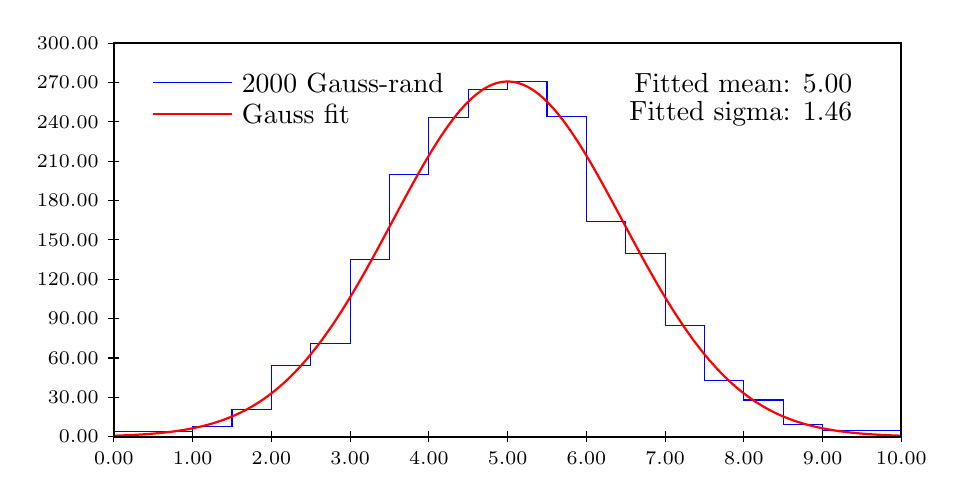
\begin{tikzpicture}[]
\begin{scope}[]
\clip (0.0,0.0) rectangle (10.0,5.0);
\begin{scope}[shift={(0.0,0.0)}]
\pgfsetxvec{\pgfpoint{1.0cm}{0cm}}
\pgfsetyvec{\pgfpoint{0cm}{0.016666668cm}}
\begin{scope}[shift={(0.0,0.0)}]
\begin{scope}[draw=blue]
\pgfpathmoveto{ \pgfpointxy {10.0} {0.0}}
\pgfpathlineto{ \pgfpointxy {10.0} {5.0}}
\pgfpathlineto{ \pgfpointxy {9.5} {5.0}}
\pgfpathlineto{ \pgfpointxy {9.5} {5.0}}
\pgfpathlineto{ \pgfpointxy {9.0} {5.0}}
\pgfpathlineto{ \pgfpointxy {9.0} {9.0}}
\pgfpathlineto{ \pgfpointxy {8.5} {9.0}}
\pgfpathlineto{ \pgfpointxy {8.5} {28.0}}
\pgfpathlineto{ \pgfpointxy {8.0} {28.0}}
\pgfpathlineto{ \pgfpointxy {8.0} {43.0}}
\pgfpathlineto{ \pgfpointxy {7.5} {43.0}}
\pgfpathlineto{ \pgfpointxy {7.5} {85.0}}
\pgfpathlineto{ \pgfpointxy {7.0} {85.0}}
\pgfpathlineto{ \pgfpointxy {7.0} {140.0}}
\pgfpathlineto{ \pgfpointxy {6.5} {140.0}}
\pgfpathlineto{ \pgfpointxy {6.5} {164.0}}
\pgfpathlineto{ \pgfpointxy {6.0} {164.0}}
\pgfpathlineto{ \pgfpointxy {6.0} {244.0}}
\pgfpathlineto{ \pgfpointxy {5.5} {244.0}}
\pgfpathlineto{ \pgfpointxy {5.5} {271.0}}
\pgfpathlineto{ \pgfpointxy {5.0} {271.0}}
\pgfpathlineto{ \pgfpointxy {5.0} {265.0}}
\pgfpathlineto{ \pgfpointxy {4.5} {265.0}}
\pgfpathlineto{ \pgfpointxy {4.5} {243.0}}
\pgfpathlineto{ \pgfpointxy {4.0} {243.0}}
\pgfpathlineto{ \pgfpointxy {4.0} {200.0}}
\pgfpathlineto{ \pgfpointxy {3.5} {200.0}}
\pgfpathlineto{ \pgfpointxy {3.5} {135.0}}
\pgfpathlineto{ \pgfpointxy {3.0} {135.0}}
\pgfpathlineto{ \pgfpointxy {3.0} {71.0}}
\pgfpathlineto{ \pgfpointxy {2.5} {71.0}}
\pgfpathlineto{ \pgfpointxy {2.5} {54.0}}
\pgfpathlineto{ \pgfpointxy {2.0} {54.0}}
\pgfpathlineto{ \pgfpointxy {2.0} {21.0}}
\pgfpathlineto{ \pgfpointxy {1.5} {21.0}}
\pgfpathlineto{ \pgfpointxy {1.5} {8.0}}
\pgfpathlineto{ \pgfpointxy {1.0} {8.0}}
\pgfpathlineto{ \pgfpointxy {1.0} {4.0}}
\pgfpathlineto{ \pgfpointxy {0.5} {4.0}}
\pgfpathlineto{ \pgfpointxy {0.5} {4.0}}
\pgfpathlineto{ \pgfpointxy {0.0} {4.0}}
\pgfpathlineto{ \pgfpointxy {0.0} {0.0}}
\pgfusepath{ stroke, }
\end{scope}
\end{scope}
\pgfsetxvec{\pgfpoint{1cm}{0cm}}
\pgfsetyvec{\pgfpoint{0cm}{1cm}}
\end{scope}
\end{scope}
\node[left] at (9.5,4.5) {Fitted mean:  5.00};
\node[left] at (9.5,4.1) {Fitted sigma:  1.46};
\begin{scope}[]
\clip (0.0,0.0) rectangle (10.0,5.0);
\begin{scope}[shift={(0.0,0.0)}]
\pgfsetxvec{\pgfpoint{1.0cm}{0cm}}
\pgfsetyvec{\pgfpoint{0cm}{0.016666668cm}}
\begin{scope}[shift={(0.0,0.0)}]
\begin{scope}[thick,red]
\pgfpathmoveto{ \pgfpointxy {0.0} {0.785533585190544}}
\pgfpathlineto{ \pgfpointxy {0.05} {0.8823944062104124}}
\pgfpathlineto{ \pgfpointxy {0.1} {0.9900410132316494}}
\pgfpathlineto{ \pgfpointxy {0.15} {1.1095224058046345}}
\pgfpathlineto{ \pgfpointxy {0.2} {1.2419708963422873}}
\pgfpathlineto{ \pgfpointxy {0.25} {1.3886065589283518}}
\pgfpathlineto{ \pgfpointxy {0.3} {1.5507416694118887}}
\pgfpathlineto{ \pgfpointxy {0.35} {1.7297851028337528}}
\pgfpathlineto{ \pgfpointxy {0.4} {1.927246650571349}}
\pgfpathlineto{ \pgfpointxy {0.45} {2.144741215868452}}
\pgfpathlineto{ \pgfpointxy {0.5} {2.383992842671168}}
\pgfpathlineto{ \pgfpointxy {0.55} {2.646838528957892}}
\pgfpathlineto{ \pgfpointxy {0.6} {2.935231772073318}}
\pgfpathlineto{ \pgfpointxy {0.65} {3.251245790000996}}
\pgfpathlineto{ \pgfpointxy {0.7} {3.5970763590868597}}
\pgfpathlineto{ \pgfpointxy {0.75} {3.9750442055123947}}
\pgfpathlineto{ \pgfpointxy {0.8} {4.387596884868998}}
\pgfpathlineto{ \pgfpointxy {0.85} {4.8373100815661525}}
\pgfpathlineto{ \pgfpointxy {0.9} {5.326888257579253}}
\pgfpathlineto{ \pgfpointxy {0.95} {5.859164578274084}}
\pgfpathlineto{ \pgfpointxy {1.0} {6.437100041802212}}
\pgfpathlineto{ \pgfpointxy {1.05} {7.063781737911131}}
\pgfpathlineto{ \pgfpointxy {1.1} {7.742420162024598}}
\pgfpathlineto{ \pgfpointxy {1.15} {8.476345511186555}}
\pgfpathlineto{ \pgfpointxy {1.2} {9.269002889991516}}
\pgfpathlineto{ \pgfpointxy {1.25} {10.12394635700542}}
\pgfpathlineto{ \pgfpointxy {1.3} {11.044831745470251}}
\pgfpathlineto{ \pgfpointxy {1.35} {12.035408196332893}}
\pgfpathlineto{ \pgfpointxy {1.4} {13.099508346888094}}
\pgfpathlineto{ \pgfpointxy {1.45} {14.241037124611898}}
\pgfpathlineto{ \pgfpointxy {1.5} {15.463959103111062}}
\pgfpathlineto{ \pgfpointxy {1.55} {16.77228438554224}}
\pgfpathlineto{ \pgfpointxy {1.6} {18.170052990364315}}
\pgfpathlineto{ \pgfpointxy {1.65} {19.661317724870088}}
\pgfpathlineto{ \pgfpointxy {1.7} {21.250125543575855}}
\pgfpathlineto{ \pgfpointxy {1.75} {22.940497401191028}}
\pgfpathlineto{ \pgfpointxy {1.8} {24.736406623493174}}
\pgfpathlineto{ \pgfpointxy {1.85} {26.64175583392414}}
\pgfpathlineto{ \pgfpointxy {1.9} {28.660352489018294}}
\pgfpathlineto{ \pgfpointxy {1.95} {30.795883091768726}}
\pgfpathlineto{ \pgfpointxy {2.0} {33.05188616861204}}
\pgfpathlineto{ \pgfpointxy {2.05} {35.431724112736475}}
\pgfpathlineto{ \pgfpointxy {2.1} {37.938554013731526}}
\pgfpathlineto{ \pgfpointxy {2.15} {40.57529761104231}}
\pgfpathlineto{ \pgfpointxy {2.2} {43.34461052608296}}
\pgfpathlineto{ \pgfpointxy {2.25} {46.248850945007725}}
\pgfpathlineto{ \pgfpointxy {2.3} {49.290047940835414}}
\pgfpathlineto{ \pgfpointxy {2.35} {52.46986963965609}}
\pgfpathlineto{ \pgfpointxy {2.4} {55.789591450800295}}
\pgfpathlineto{ \pgfpointxy {2.45} {59.25006459489787}}
\pgfpathlineto{ \pgfpointxy {2.5} {62.85168517646614}}
\pgfpathlineto{ \pgfpointxy {2.55} {66.5943640588275}}
\pgfpathlineto{ \pgfpointxy {2.6} {70.47749780853638}}
\pgfpathlineto{ \pgfpointxy {2.65} {74.49994098389061}}
\pgfpathlineto{ \pgfpointxy {2.7} {78.65998004730363}}
\pgfpathlineto{ \pgfpointxy {2.75} {82.9553091841374}}
\pgfpathlineto{ \pgfpointxy {2.8} {87.38300831087108}}
\pgfpathlineto{ \pgfpointxy {2.85} {91.93952355305386}}
\pgfpathlineto{ \pgfpointxy {2.9} {96.62065046824108}}
\pgfpathlineto{ \pgfpointxy {2.95} {101.42152028093761}}
\pgfpathlineto{ \pgfpointxy {3.0} {106.33658938540171}}
\pgfpathlineto{ \pgfpointxy {3.05} {111.35963235796345}}
\pgfpathlineto{ \pgfpointxy {3.1} {116.48373870327391}}
\pgfpathlineto{ \pgfpointxy {3.15} {121.70131353866445}}
\pgfpathlineto{ \pgfpointxy {3.2} {127.00408239762504}}
\pgfpathlineto{ \pgfpointxy {3.25} {132.38310030741803}}
\pgfpathlineto{ \pgfpointxy {3.3} {137.82876526717794}}
\pgfpathlineto{ \pgfpointxy {3.35} {143.3308362216892}}
\pgfpathlineto{ \pgfpointxy {3.4} {148.87845559261598}}
\pgfpathlineto{ \pgfpointxy {3.45} {154.4601763935346}}
\pgfpathlineto{ \pgfpointxy {3.5} {160.06399391798755}}
\pgfpathlineto{ \pgfpointxy {3.55} {165.67738195127163}}
\pgfpathlineto{ \pgfpointxy {3.6} {171.28733341714147}}
\pgfpathlineto{ \pgfpointxy {3.65} {176.88040533044696}}
\pgfpathlineto{ \pgfpointxy {3.7} {182.4427678863249}}
\pgfpathlineto{ \pgfpointxy {3.75} {187.96025747636367}}
\pgfpathlineto{ \pgfpointxy {3.8} {193.4184333825861}}
\pgfpathlineto{ \pgfpointxy {3.85} {198.8026378615926}}
\pgfpathlineto{ \pgfpointxy {3.9} {204.0980592942233}}
\pgfpathlineto{ \pgfpointxy {3.95} {209.2897980410712}}
\pgfpathlineto{ \pgfpointxy {4.0} {214.36293461154008}}
\pgfpathlineto{ \pgfpointxy {4.05} {219.30259972431023}}
\pgfpathlineto{ \pgfpointxy {4.1} {224.09404581043842}}
\pgfpathlineto{ \pgfpointxy {4.15} {228.7227194872519}}
\pgfpathlineto{ \pgfpointxy {4.2} {233.1743345120225}}
\pgfpathlineto{ \pgfpointxy {4.25} {237.43494470943358}}
\pgfpathlineto{ \pgfpointxy {4.3} {241.4910163563196}}
\pgfpathlineto{ \pgfpointxy {4.35} {245.32949950128543}}
\pgfpathlineto{ \pgfpointxy {4.4} {248.93789769574337}}
\pgfpathlineto{ \pgfpointxy {4.45} {252.30433561675085}}
\pgfpathlineto{ \pgfpointxy {4.5} {255.4176240708332}}
\pgfpathlineto{ \pgfpointxy {4.55} {258.26732188172053}}
\pgfpathlineto{ \pgfpointxy {4.6} {260.84379418355206}}
\pgfpathlineto{ \pgfpointxy {4.65} {263.13826666446903}}
\pgfpathlineto{ \pgfpointxy {4.7} {265.14287533345066}}
\pgfpathlineto{ \pgfpointxy {4.75} {266.8507114154981}}
\pgfpathlineto{ \pgfpointxy {4.8} {268.25586101655}}
\pgfpathlineto{ \pgfpointxy {4.85} {269.35343923947187}}
\pgfpathlineto{ \pgfpointxy {4.9} {270.1396184757107}}
\pgfpathlineto{ \pgfpointxy {4.95} {270.6116506433102}}
\pgfpathlineto{ \pgfpointxy {5.0} {270.76788319047864}}
\pgfpathlineto{ \pgfpointxy {5.05} {270.6077687342832}}
\pgfpathlineto{ \pgfpointxy {5.1} {270.1318682557956}}
\pgfpathlineto{ \pgfpointxy {5.15} {269.3418478255878}}
\pgfpathlineto{ \pgfpointxy {5.2} {268.24046888632785}}
\pgfpathlineto{ \pgfpointxy {5.25} {266.8315721717906}}
\pgfpathlineto{ \pgfpointxy {5.3} {265.1200553933392}}
\pgfpathlineto{ \pgfpointxy {5.35} {263.11184487529204}}
\pgfpathlineto{ \pgfpointxy {5.4} {260.81386136906104}}
\pgfpathlineto{ \pgfpointxy {5.45} {258.23398032201965}}
\pgfpathlineto{ \pgfpointxy {5.5} {255.38098692026887}}
\pgfpathlineto{ \pgfpointxy {5.55} {252.26452626438723}}
\pgfpathlineto{ \pgfpointxy {5.6} {248.89504907347904}}
\pgfpathlineto{ \pgfpointxy {5.65} {245.28375334503724}}
\pgfpathlineto{ \pgfpointxy {5.7} {241.44252242601453}}
\pgfpathlineto{ \pgfpointxy {5.75} {237.38385997380678}}
\pgfpathlineto{ \pgfpointxy {5.8} {233.12082230441845}}
\pgfpathlineto{ \pgfpointxy {5.85} {228.66694863876333}}
\pgfpathlineto{ \pgfpointxy {5.9} {224.03618976679525}}
\pgfpathlineto{ \pgfpointxy {5.95} {219.2428356529474}}
\pgfpathlineto{ \pgfpointxy {6.0} {214.3014425052294}}
\pgfpathlineto{ \pgfpointxy {6.05} {209.22675982440097}}
\pgfpathlineto{ \pgfpointxy {6.1} {204.03365793905297}}
\pgfpathlineto{ \pgfpointxy {6.15} {198.73705651739786}}
\pgfpathlineto{ \pgfpointxy {6.2} {193.35185452735166}}
\pgfpathlineto{ \pgfpointxy {6.25} {187.8928620933718}}
\pgfpathlineto{ \pgfpointxy {6.3} {182.3747346718441}}
\pgfpathlineto{ \pgfpointxy {6.35} {176.81190993693747}}
\pgfpathlineto{ \pgfpointxy {6.4} {171.21854773617946}}
\pgfpathlineto{ \pgfpointxy {6.45} {165.6084734399515}}
\pgfpathlineto{ \pgfpointxy {6.5} {159.99512497209525}}
\pgfpathlineto{ \pgfpointxy {6.55} {154.39150377030742}}
\pgfpathlineto{ \pgfpointxy {6.6} {148.81012988541192}}
\pgfpathlineto{ \pgfpointxy {6.65} {143.26300138839366}}
\pgfpathlineto{ \pgfpointxy {6.7} {137.76155821368138}}
\pgfpathlineto{ \pgfpointxy {6.75} {132.31665052700623}}
\pgfpathlineto{ \pgfpointxy {6.8} {126.93851166664665}}
\pgfpathlineto{ \pgfpointxy {6.85} {121.63673566837342}}
\pgfpathlineto{ \pgfpointxy {6.9} {116.4202593472993}}
\pgfpathlineto{ \pgfpointxy {6.95} {111.29734887443767}}
\pgfpathlineto{ \pgfpointxy {7.0} {106.27559075237848}}
\pgfpathlineto{ \pgfpointxy {7.05} {101.36188706336671}}
\pgfpathlineto{ \pgfpointxy {7.1} {96.56245483442952}}
\pgfpathlineto{ \pgfpointxy {7.15} {91.88282933824159}}
\pgfpathlineto{ \pgfpointxy {7.2} {87.32787112528398}}
\pgfpathlineto{ \pgfpointxy {7.25} {82.90177656264828}}
\pgfpathlineto{ \pgfpointxy {7.3} {78.60809163764216}}
\pgfpathlineto{ \pgfpointxy {7.35} {74.44972877018493}}
\pgfpathlineto{ \pgfpointxy {7.4} {70.4289863668524}}
\pgfpathlineto{ \pgfpointxy {7.45} {66.5475708412896}}
\pgfpathlineto{ \pgfpointxy {7.5} {62.80662082049553}}
\pgfpathlineto{ \pgfpointxy {7.55} {59.20673325409326}}
\pgfpathlineto{ \pgfpointxy {7.6} {55.74799114400455}}
\pgfpathlineto{ \pgfpointxy {7.65} {52.42999261480181}}
\pgfpathlineto{ \pgfpointxy {7.7} {49.25188105024186}}
\pgfpathlineto{ \pgfpointxy {7.75} {46.2123760289026}}
\pgfpathlineto{ \pgfpointxy {7.8} {43.30980480125177}}
\pgfpathlineto{ \pgfpointxy {7.85} {40.54213406165323}}
\pgfpathlineto{ \pgfpointxy {7.9} {37.90700178154938}}
\pgfpathlineto{ \pgfpointxy {7.95} {35.40174888411922}}
\pgfpathlineto{ \pgfpointxy {8.0} {33.02345055587413}}
\pgfpathlineto{ \pgfpointxy {8.05} {30.768947006698582}}
\pgfpathlineto{ \pgfpointxy {8.1} {28.6348735065443}}
\pgfpathlineto{ \pgfpointxy {8.15} {26.61768954413513}}
\pgfpathlineto{ \pgfpointxy {8.2} {24.713706970436572}}
\pgfpathlineto{ \pgfpointxy {8.25} {22.91911700708104}}
\pgfpathlineto{ \pgfpointxy {8.3} {21.230016017259846}}
\pgfpathlineto{ \pgfpointxy {8.35} {19.642429953603866}}
\pgfpathlineto{ \pgfpointxy {8.4} {18.152337414149354}}
\pgfpathlineto{ \pgfpointxy {8.45} {16.75569125346978}}
\pgfpathlineto{ \pgfpointxy {8.5} {15.448438711340048}}
\pgfpathlineto{ \pgfpointxy {8.55} {14.226540035781417}}
\pgfpathlineto{ \pgfpointxy {8.6} {13.08598559092523}}
\pgfpathlineto{ \pgfpointxy {8.65} {12.022811452766204}}
\pgfpathlineto{ \pgfpointxy {8.7} {11.033113507495788}}
\pgfpathlineto{ \pgfpointxy {8.75} {10.1130600776746}}
\pgfpathlineto{ \pgfpointxy {8.8} {9.258903111001242}}
\pgfpathlineto{ \pgfpointxy {8.85} {8.4669879748478}}
\pgfpathlineto{ \pgfpointxy {8.9} {7.733761907069523}}
\pgfpathlineto{ \pgfpointxy {8.95} {7.055781179870019}}
\pgfpathlineto{ \pgfpointxy {9.0} {6.429717038738498}}
\pgfpathlineto{ \pgfpointxy {9.05} {5.852360482713078}}
\pgfpathlineto{ \pgfpointxy {9.1} {5.320625955499768}}
\pgfpathlineto{ \pgfpointxy {9.15} {4.8315540193486735}}
\pgfpathlineto{ \pgfpointxy {9.2} {4.382313085107549}}
\pgfpathlineto{ \pgfpointxy {9.25} {3.9702002726017023}}
\pgfpathlineto{ \pgfpointxy {9.3} {3.5926414754922513}}
\pgfpathlineto{ \pgfpointxy {9.35} {3.2471907041067585}}
\pgfpathlineto{ \pgfpointxy {9.4} {2.931528778486455}}
\pgfpathlineto{ \pgfpointxy {9.45} {2.643461442119739}}
\pgfpathlineto{ \pgfpointxy {9.5} {2.380916964599145}}
\pgfpathlineto{ \pgfpointxy {9.55} {2.1419432988161606}}
\pgfpathlineto{ \pgfpointxy {9.6} {1.9247048553571429}}
\pgfpathlineto{ \pgfpointxy {9.65} {1.7274789535470048}}
\pgfpathlineto{ \pgfpointxy {9.7} {1.5486520051633315}}
\pgfpathlineto{ \pgfpointxy {9.75} {1.3867154832659307}}
\pgfpathlineto{ \pgfpointxy {9.8} {1.2402617249087116}}
\pgfpathlineto{ \pgfpointxy {9.85} {1.1079796127665273}}
\pgfpathlineto{ \pgfpointxy {9.9} {0.9886501769645344}}
\pgfpathlineto{ \pgfpointxy {9.95} {0.8811421546783109}}
\pgfpathlineto{ \pgfpointxy {10.0} {0.7844075414145795}}
\pgfusepath{ stroke, }
\end{scope}
\end{scope}
\pgfsetxvec{\pgfpoint{1cm}{0cm}}
\pgfsetyvec{\pgfpoint{0cm}{1cm}}
\end{scope}
\end{scope}
\begin{scope}[shift={(0.0,0.0)}]
\pgfsetxvec{\pgfpoint{1.0cm}{0cm}}
\pgfsetyvec{\pgfpoint{0cm}{0.016666668cm}}
\begin{scope}[shift={(0.0,0.0)}]
\begin{scope}[yshift=0cm]
\draw[black] [shift={(0.0,0.0)}] (0,2pt) -- (0,-2pt) node[below]{ \scriptsize{\num[round-mode=places,round-precision=2]{0}}};
\draw[black] [shift={(1.0,0.0)}] (0,2pt) -- (0,-2pt) node[below]{ \scriptsize{\num[round-mode=places,round-precision=2]{1}}};
\draw[black] [shift={(2.0,0.0)}] (0,2pt) -- (0,-2pt) node[below]{ \scriptsize{\num[round-mode=places,round-precision=2]{2}}};
\draw[black] [shift={(3.0,0.0)}] (0,2pt) -- (0,-2pt) node[below]{ \scriptsize{\num[round-mode=places,round-precision=2]{3}}};
\draw[black] [shift={(4.0,0.0)}] (0,2pt) -- (0,-2pt) node[below]{ \scriptsize{\num[round-mode=places,round-precision=2]{4}}};
\draw[black] [shift={(5.0,0.0)}] (0,2pt) -- (0,-2pt) node[below]{ \scriptsize{\num[round-mode=places,round-precision=2]{5}}};
\draw[black] [shift={(6.0,0.0)}] (0,2pt) -- (0,-2pt) node[below]{ \scriptsize{\num[round-mode=places,round-precision=2]{6}}};
\draw[black] [shift={(7.0,0.0)}] (0,2pt) -- (0,-2pt) node[below]{ \scriptsize{\num[round-mode=places,round-precision=2]{7}}};
\draw[black] [shift={(8.0,0.0)}] (0,2pt) -- (0,-2pt) node[below]{ \scriptsize{\num[round-mode=places,round-precision=2]{8}}};
\draw[black] [shift={(9.0,0.0)}] (0,2pt) -- (0,-2pt) node[below]{ \scriptsize{\num[round-mode=places,round-precision=2]{9}}};
\draw[black] [shift={(10.0,0.0)}] (0,2pt) -- (0,-2pt) node[below]{ \scriptsize{\num[round-mode=places,round-precision=2]{10}}};
\end{scope}
\begin{scope}[xshift=0cm]
\draw[black] [shift={(0.0,0.0)}] (2pt,0) -- (-2pt,0) node[left]{ \scriptsize{\num[round-mode=places,round-precision=2]{0}}};
\draw[black] [shift={(0.0,30.0)}] (2pt,0) -- (-2pt,0) node[left]{ \scriptsize{\num[round-mode=places,round-precision=2]{30}}};
\draw[black] [shift={(0.0,60.0)}] (2pt,0) -- (-2pt,0) node[left]{ \scriptsize{\num[round-mode=places,round-precision=2]{60}}};
\draw[black] [shift={(0.0,90.0)}] (2pt,0) -- (-2pt,0) node[left]{ \scriptsize{\num[round-mode=places,round-precision=2]{90}}};
\draw[black] [shift={(0.0,120.0)}] (2pt,0) -- (-2pt,0) node[left]{ \scriptsize{\num[round-mode=places,round-precision=2]{120}}};
\draw[black] [shift={(0.0,150.0)}] (2pt,0) -- (-2pt,0) node[left]{ \scriptsize{\num[round-mode=places,round-precision=2]{150}}};
\draw[black] [shift={(0.0,180.0)}] (2pt,0) -- (-2pt,0) node[left]{ \scriptsize{\num[round-mode=places,round-precision=2]{180}}};
\draw[black] [shift={(0.0,210.0)}] (2pt,0) -- (-2pt,0) node[left]{ \scriptsize{\num[round-mode=places,round-precision=2]{210}}};
\draw[black] [shift={(0.0,240.0)}] (2pt,0) -- (-2pt,0) node[left]{ \scriptsize{\num[round-mode=places,round-precision=2]{240}}};
\draw[black] [shift={(0.0,270.0)}] (2pt,0) -- (-2pt,0) node[left]{ \scriptsize{\num[round-mode=places,round-precision=2]{270}}};
\draw[black] [shift={(0.0,300.0)}] (2pt,0) -- (-2pt,0) node[left]{ \scriptsize{\num[round-mode=places,round-precision=2]{300}}};
\end{scope}
\end{scope}
\pgfsetxvec{\pgfpoint{1cm}{0cm}}
\pgfsetyvec{\pgfpoint{0cm}{1cm}}
\end{scope}
\draw[draw=blue,fill=blue] (0.5,4.5) -- (1.5,4.5);
\node[right,] at (1.5,4.5) {2000 Gauss-rand};
\draw[thick,red] (0.5,4.1) -- (1.5,4.1);
\node[right,] at (1.5,4.1) {Gauss fit};
\begin{scope}[thick,black,fill=white]
\pgfpathmoveto{ \pgfpointxy {0.0} {0.0}}
\pgfpathlineto{ \pgfpointxy {10.0} {0.0}}
\pgfpathlineto{ \pgfpointxy {10.0} {5.0}}
\pgfpathlineto{ \pgfpointxy {0.0} {5.0}}
\pgfpathclose
\pgfusepath{ stroke, }
\end{scope}
\end{tikzpicture}
%%% Local Variables: 
%%% mode: latex 
%%% TeX-master: "master" 
%%% End:


  \caption{The Gaussian function fitted to histogram made from 2000 gaussian random numbers}
\end{figure}

\begin{figure}[H]
  \centering
  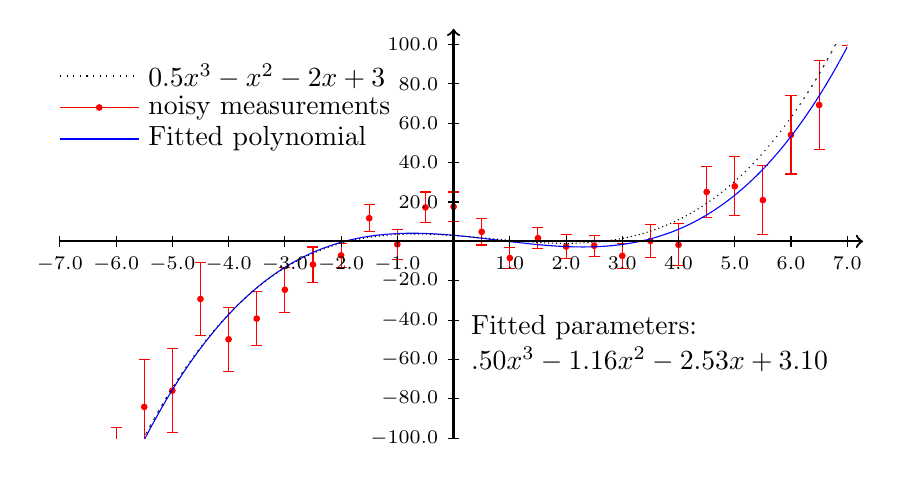
\begin{tikzpicture}
\begin{scope}[]
\clip (0,0) rectangle (10,5);
\draw[draw=red,fill=red] (-2.142857,-13.690766900522135) -- (-2.142857,-11.088684470629271);
\draw[draw=red,fill=red] (-2.142857,-12.389725685575703) circle(1pt); 
\draw[draw=red,fill=red] (-2.142857cm -2pt,-13.690766900522135) -- (-2.142857cm + 2pt,-13.690766900522135);
\draw[draw=red,fill=red] (-2.142857cm -2pt,-11.088684470629271) -- (-2.142857cm + 2pt,-11.088684470629271);
\draw[draw=red,fill=red] (-1.7857143,-11.547360643679772) -- (-1.7857143,-9.118151142533682);
\draw[draw=red,fill=red] (-1.7857143,-10.332755893106727) circle(1pt); 
\draw[draw=red,fill=red] (-1.7857143cm -2pt,-11.547360643679772) -- (-1.7857143cm + 2pt,-11.547360643679772);
\draw[draw=red,fill=red] (-1.7857143cm -2pt,-9.118151142533682) -- (-1.7857143cm + 2pt,-9.118151142533682);
\draw[draw=red,fill=red] (-1.4285715,-9.64862972900496) -- (-1.4285715,-7.388289951201308);
\draw[draw=red,fill=red] (-1.4285715,-8.518459840103134) circle(1pt); 
\draw[draw=red,fill=red] (-1.4285715cm -2pt,-9.64862972900496) -- (-1.4285715cm + 2pt,-9.64862972900496);
\draw[draw=red,fill=red] (-1.4285715cm -2pt,-7.388289951201308) -- (-1.4285715cm + 2pt,-7.388289951201308);
\draw[draw=red,fill=red] (-1.0714285,-7.637085601637203) -- (-1.0714285,-5.5415315929104665);
\draw[draw=red,fill=red] (-1.0714285,-6.589308597273835) circle(1pt); 
\draw[draw=red,fill=red] (-1.0714285cm -2pt,-7.637085601637203) -- (-1.0714285cm + 2pt,-7.637085601637203);
\draw[draw=red,fill=red] (-1.0714285cm -2pt,-5.5415315929104665) -- (-1.0714285cm + 2pt,-5.5415315929104665);
\draw[draw=red,fill=red] (-0.71428573,-4.594043342574411) -- (-0.71428573,-2.659108185284664);
\draw[draw=red,fill=red] (-0.71428573,-3.6265757639295373) circle(1pt); 
\draw[draw=red,fill=red] (-0.71428573cm -2pt,-4.594043342574411) -- (-0.71428573cm + 2pt,-4.594043342574411);
\draw[draw=red,fill=red] (-0.71428573cm -2pt,-2.659108185284664) -- (-0.71428573cm + 2pt,-2.659108185284664);
\draw[draw=red,fill=red] (-0.35714287,-5.796105953276756) -- (-0.35714287,-4.017538564788067);
\draw[draw=red,fill=red] (-0.35714287,-4.9068222590324115) circle(1pt); 
\draw[draw=red,fill=red] (-0.35714287cm -2pt,-5.796105953276756) -- (-0.35714287cm + 2pt,-5.796105953276756);
\draw[draw=red,fill=red] (-0.35714287cm -2pt,-4.017538564788067) -- (-0.35714287cm + 2pt,-4.017538564788067);
\draw[draw=red,fill=red] (0.0,-2.962409254330664) -- (0.0,-1.335874992561954);
\draw[draw=red,fill=red] (0.0,-2.149142123446309) circle(1pt); 
\draw[draw=red,fill=red] (0.0cm -2pt,-2.962409254330664) -- (0.0cm + 2pt,-2.962409254330664);
\draw[draw=red,fill=red] (0.0cm -2pt,-1.335874992561954) -- (0.0cm + 2pt,-1.335874992561954);
\draw[draw=red,fill=red] (0.35714287,-2.3595412915979326) -- (0.35714287,-0.8806257353550662);
\draw[draw=red,fill=red] (0.35714287,-1.6200835134764993) circle(1pt); 
\draw[draw=red,fill=red] (0.35714287cm -2pt,-2.3595412915979326) -- (0.35714287cm + 2pt,-2.3595412915979326);
\draw[draw=red,fill=red] (0.35714287cm -2pt,-0.8806257353550662) -- (0.35714287cm + 2pt,-0.8806257353550662);
\draw[draw=red,fill=red] (0.71428573,-1.199661460258557) -- (0.71428573,0.13612020890149779);
\draw[draw=red,fill=red] (0.71428573,-0.5317706256785296) circle(1pt); 
\draw[draw=red,fill=red] (0.71428573cm -2pt,-1.199661460258557) -- (0.71428573cm + 2pt,-1.199661460258557);
\draw[draw=red,fill=red] (0.71428573cm -2pt,0.13612020890149779) -- (0.71428573cm + 2pt,0.13612020890149779);
\draw[draw=red,fill=red] (1.0714285,-0.20121218473837588) -- (1.0714285,0.9959713490205806);
\draw[draw=red,fill=red] (1.0714285,0.39737958214110236) circle(1pt); 
\draw[draw=red,fill=red] (1.0714285cm -2pt,-0.20121218473837588) -- (1.0714285cm + 2pt,-0.20121218473837588);
\draw[draw=red,fill=red] (1.0714285cm -2pt,0.9959713490205806) -- (1.0714285cm + 2pt,0.9959713490205806);
\draw[draw=red,fill=red] (1.4285715,0.07283499514594083) -- (1.4285715,1.1359688202275442);
\draw[draw=red,fill=red] (1.4285715,0.6044019076867425) circle(1pt); 
\draw[draw=red,fill=red] (1.4285715cm -2pt,0.07283499514594083) -- (1.4285715cm + 2pt,0.07283499514594083);
\draw[draw=red,fill=red] (1.4285715cm -2pt,1.1359688202275442) -- (1.4285715cm + 2pt,1.1359688202275442);
\draw[draw=red,fill=red] (1.7857143,1.3014636063312879) -- (1.7857143,2.2350336438873484);
\draw[draw=red,fill=red] (1.7857143,1.7682486251093181) circle(1pt); 
\draw[draw=red,fill=red] (1.7857143cm -2pt,1.3014636063312879) -- (1.7857143cm + 2pt,1.3014636063312879);
\draw[draw=red,fill=red] (1.7857143cm -2pt,2.2350336438873484) -- (1.7857143cm + 2pt,2.2350336438873484);
\draw[draw=red,fill=red] (2.142857,0.8525355883035404) -- (2.142857,1.6608118413333621);
\draw[draw=red,fill=red] (2.142857,1.2566737148184512) circle(1pt); 
\draw[draw=red,fill=red] (2.142857cm -2pt,0.8525355883035404) -- (2.142857cm + 2pt,0.8525355883035404);
\draw[draw=red,fill=red] (2.142857cm -2pt,1.6608118413333621) -- (2.142857cm + 2pt,1.6608118413333621);
\draw[draw=red,fill=red] (2.5,1.1758875509572513) -- (2.5,1.8625856093055457);
\draw[draw=red,fill=red] (2.5,1.5192365801313985) circle(1pt); 
\draw[draw=red,fill=red] (2.5cm -2pt,1.1758875509572513) -- (2.5cm + 2pt,1.1758875509572513);
\draw[draw=red,fill=red] (2.5cm -2pt,1.8625856093055457) -- (2.5cm + 2pt,1.8625856093055457);
\draw[draw=red,fill=red] (2.857143,1.6017864499030297) -- (2.857143,2.169209911320506);
\draw[draw=red,fill=red] (2.857143,1.8854981806117679) circle(1pt); 
\draw[draw=red,fill=red] (2.857143cm -2pt,1.6017864499030297) -- (2.857143cm + 2pt,1.6017864499030297);
\draw[draw=red,fill=red] (2.857143cm -2pt,2.169209911320506) -- (2.857143cm + 2pt,2.169209911320506);
\draw[draw=red,fill=red] (3.2142859,1.9826782299002694) -- (3.2142859,2.428899674945172);
\draw[draw=red,fill=red] (3.2142859,2.2057889524227208) circle(1pt); 
\draw[draw=red,fill=red] (3.2142859cm -2pt,1.9826782299002694) -- (3.2142859cm + 2pt,1.9826782299002694);
\draw[draw=red,fill=red] (3.2142859cm -2pt,2.428899674945172) -- (3.2142859cm + 2pt,2.428899674945172);
\draw[draw=red,fill=red] (3.5714285,2.1719053314991754) -- (3.5714285,2.4719053314991752);
\draw[draw=red,fill=red] (3.5714285,2.3219053314991753) circle(1pt); 
\draw[draw=red,fill=red] (3.5714285cm -2pt,2.1719053314991754) -- (3.5714285cm + 2pt,2.1719053314991754);
\draw[draw=red,fill=red] (3.5714285cm -2pt,2.4719053314991752) -- (3.5714285cm + 2pt,2.4719053314991752);
\draw[draw=red,fill=red] (3.9285715,2.622904496231831) -- (3.9285715,2.9665185623952812);
\draw[draw=red,fill=red] (3.9285715,2.794711529313556) circle(1pt); 
\draw[draw=red,fill=red] (3.9285715cm -2pt,2.622904496231831) -- (3.9285715cm + 2pt,2.622904496231831);
\draw[draw=red,fill=red] (3.9285715cm -2pt,2.9665185623952812) -- (3.9285715cm + 2pt,2.9665185623952812);
\draw[draw=red,fill=red] (4.285714,2.268574659499892) -- (4.285714,2.6556575288385895);
\draw[draw=red,fill=red] (4.285714,2.462116094169241) circle(1pt); 
\draw[draw=red,fill=red] (4.285714cm -2pt,2.268574659499892) -- (4.285714cm + 2pt,2.268574659499892);
\draw[draw=red,fill=red] (4.285714cm -2pt,2.6556575288385895) -- (4.285714cm + 2pt,2.6556575288385895);
\draw[draw=red,fill=red] (4.642857,2.7353486391801107) -- (4.642857,3.127377282876826);
\draw[draw=red,fill=red] (4.642857,2.9313629610284684) circle(1pt); 
\draw[draw=red,fill=red] (4.642857cm -2pt,2.7353486391801107) -- (4.642857cm + 2pt,2.7353486391801107);
\draw[draw=red,fill=red] (4.642857cm -2pt,3.127377282876826) -- (4.642857cm + 2pt,3.127377282876826);
\draw[draw=red,fill=red] (5.0,2.753229322304523) -- (5.0,3.126434403061411);
\draw[draw=red,fill=red] (5.0,2.939831862682967) circle(1pt); 
\draw[draw=red,fill=red] (5.0cm -2pt,2.753229322304523) -- (5.0cm + 2pt,2.753229322304523);
\draw[draw=red,fill=red] (5.0cm -2pt,3.126434403061411) -- (5.0cm + 2pt,3.126434403061411);
\draw[draw=red,fill=red] (5.357143,2.4538980485227913) -- (5.357143,2.788527168701154);
\draw[draw=red,fill=red] (5.357143,2.6212126086119727) circle(1pt); 
\draw[draw=red,fill=red] (5.357143cm -2pt,2.4538980485227913) -- (5.357143cm + 2pt,2.4538980485227913);
\draw[draw=red,fill=red] (5.357143cm -2pt,2.788527168701154) -- (5.357143cm + 2pt,2.788527168701154);
\draw[draw=red,fill=red] (5.714286,2.152866155952158) -- (5.714286,2.4235768340708126);
\draw[draw=red,fill=red] (5.714286,2.288221495011485) circle(1pt); 
\draw[draw=red,fill=red] (5.714286cm -2pt,2.152866155952158) -- (5.714286cm + 2pt,2.152866155952158);
\draw[draw=red,fill=red] (5.714286cm -2pt,2.4235768340708126) -- (5.714286cm + 2pt,2.4235768340708126);
\draw[draw=red,fill=red] (6.071429,2.404394903388126) -- (6.071429,2.6793949033881264);
\draw[draw=red,fill=red] (6.071429,2.541894903388126) circle(1pt); 
\draw[draw=red,fill=red] (6.071429cm -2pt,2.404394903388126) -- (6.071429cm + 2pt,2.404394903388126);
\draw[draw=red,fill=red] (6.071429cm -2pt,2.6793949033881264) -- (6.071429cm + 2pt,2.6793949033881264);
\draw[draw=red,fill=red] (6.4285717,2.2844725706941964) -- (6.4285717,2.5844725706941962);
\draw[draw=red,fill=red] (6.4285717,2.4344725706941963) circle(1pt); 
\draw[draw=red,fill=red] (6.4285717cm -2pt,2.2844725706941964) -- (6.4285717cm + 2pt,2.2844725706941964);
\draw[draw=red,fill=red] (6.4285717cm -2pt,2.5844725706941962) -- (6.4285717cm + 2pt,2.5844725706941962);
\draw[draw=red,fill=red] (6.7857146,2.311012057325212) -- (6.7857146,2.5771558401018266);
\draw[draw=red,fill=red] (6.7857146,2.4440839487135193) circle(1pt); 
\draw[draw=red,fill=red] (6.7857146cm -2pt,2.311012057325212) -- (6.7857146cm + 2pt,2.311012057325212);
\draw[draw=red,fill=red] (6.7857146cm -2pt,2.5771558401018266) -- (6.7857146cm + 2pt,2.5771558401018266);
\draw[draw=red,fill=red] (7.142857,2.1554091573639695) -- (7.142857,2.4778836445031285);
\draw[draw=red,fill=red] (7.142857,2.316646400933549) circle(1pt); 
\draw[draw=red,fill=red] (7.142857cm -2pt,2.1554091573639695) -- (7.142857cm + 2pt,2.1554091573639695);
\draw[draw=red,fill=red] (7.142857cm -2pt,2.4778836445031285) -- (7.142857cm + 2pt,2.4778836445031285);
\draw[draw=red,fill=red] (7.5,2.2919468922135207) -- (7.5,2.7197077316921283);
\draw[draw=red,fill=red] (7.5,2.5058273119528245) circle(1pt); 
\draw[draw=red,fill=red] (7.5cm -2pt,2.2919468922135207) -- (7.5cm + 2pt,2.2919468922135207);
\draw[draw=red,fill=red] (7.5cm -2pt,2.7197077316921283) -- (7.5cm + 2pt,2.7197077316921283);
\draw[draw=red,fill=red] (7.857143,2.190573053492995) -- (7.857143,2.722235532528535);
\draw[draw=red,fill=red] (7.857143,2.456404293010765) circle(1pt); 
\draw[draw=red,fill=red] (7.857143cm -2pt,2.190573053492995) -- (7.857143cm + 2pt,2.190573053492995);
\draw[draw=red,fill=red] (7.857143cm -2pt,2.722235532528535) -- (7.857143cm + 2pt,2.722235532528535);
\draw[draw=red,fill=red] (8.214286,2.807793977537827) -- (8.214286,3.447253873319001);
\draw[draw=red,fill=red] (8.214286,3.127523925428414) circle(1pt); 
\draw[draw=red,fill=red] (8.214286cm -2pt,2.807793977537827) -- (8.214286cm + 2pt,2.807793977537827);
\draw[draw=red,fill=red] (8.214286cm -2pt,3.447253873319001) -- (8.214286cm + 2pt,3.447253873319001);
\draw[draw=red,fill=red] (8.571428,2.8235369533398798) -- (8.571428,3.5758050041992426);
\draw[draw=red,fill=red] (8.571428,3.199670978769561) circle(1pt); 
\draw[draw=red,fill=red] (8.571428cm -2pt,2.8235369533398798) -- (8.571428cm + 2pt,2.8235369533398798);
\draw[draw=red,fill=red] (8.571428cm -2pt,3.5758050041992426) -- (8.571428cm + 2pt,3.5758050041992426);
\draw[draw=red,fill=red] (8.928572,2.5894682162756566) -- (8.928572,3.459822600165253);
\draw[draw=red,fill=red] (8.928572,3.024645408220455) circle(1pt); 
\draw[draw=red,fill=red] (8.928572cm -2pt,2.5894682162756566) -- (8.928572cm + 2pt,2.5894682162756566);
\draw[draw=red,fill=red] (8.928572cm -2pt,3.459822600165253) -- (8.928572cm + 2pt,3.459822600165253);
\draw[draw=red,fill=red] (9.285714,3.3555610683946355) -- (9.285714,4.349286461714013);
\draw[draw=red,fill=red] (9.285714,3.8524237650543243) circle(1pt); 
\draw[draw=red,fill=red] (9.285714cm -2pt,3.3555610683946355) -- (9.285714cm + 2pt,3.3555610683946355);
\draw[draw=red,fill=red] (9.285714cm -2pt,4.349286461714013) -- (9.285714cm + 2pt,4.349286461714013);
\draw[draw=red,fill=red] (9.642858,3.670924469182596) -- (9.642858,4.793217806467432);
\draw[draw=red,fill=red] (9.642858,4.232071137825014) circle(1pt); 
\draw[draw=red,fill=red] (9.642858cm -2pt,3.670924469182596) -- (9.642858cm + 2pt,3.670924469182596);
\draw[draw=red,fill=red] (9.642858cm -2pt,4.793217806467432) -- (9.642858cm + 2pt,4.793217806467432);
\draw[draw=red,fill=red] (10.0,4.987673323439317) -- (10.0,6.24360892753646);
\draw[draw=red,fill=red] (10.0,5.615641125487889) circle(1pt); 
\draw[draw=red,fill=red] (10.0cm -2pt,4.987673323439317) -- (10.0cm + 2pt,4.987673323439317);
\draw[draw=red,fill=red] (10.0cm -2pt,6.24360892753646) -- (10.0cm + 2pt,6.24360892753646);
\draw[draw=red,fill=red] (10.357143,4.515341770846103) -- (10.357143,5.909860502386131);
\draw[draw=red,fill=red] (10.357143,5.212601136616117) circle(1pt); 
\draw[draw=red,fill=red] (10.357143cm -2pt,4.515341770846103) -- (10.357143cm + 2pt,4.515341770846103);
\draw[draw=red,fill=red] (10.357143cm -2pt,5.909860502386131) -- (10.357143cm + 2pt,5.909860502386131);
\draw[draw=red,fill=red] (10.714286,6.270108949441174) -- (10.714286,7.808017765467139);
\draw[draw=red,fill=red] (10.714286,7.039063357454157) circle(1pt); 
\draw[draw=red,fill=red] (10.714286cm -2pt,6.270108949441174) -- (10.714286cm + 2pt,6.270108949441174);
\draw[draw=red,fill=red] (10.714286cm -2pt,7.808017765467139) -- (10.714286cm + 2pt,7.808017765467139);
\draw[draw=red,fill=red] (11.071428,8.310451887182419) -- (11.071428,9.996427997353775);
\draw[draw=red,fill=red] (11.071428,9.153439942268097) circle(1pt); 
\draw[draw=red,fill=red] (11.071428cm -2pt,8.310451887182419) -- (11.071428cm + 2pt,8.310451887182419);
\draw[draw=red,fill=red] (11.071428cm -2pt,9.996427997353775) -- (11.071428cm + 2pt,9.996427997353775);
\draw[draw=red,fill=red] (11.428572,7.494686295042708) -- (11.428572,9.333283255860103);
\draw[draw=red,fill=red] (11.428572,8.413984775451405) circle(1pt); 
\draw[draw=red,fill=red] (11.428572cm -2pt,7.494686295042708) -- (11.428572cm + 2pt,7.494686295042708);
\draw[draw=red,fill=red] (11.428572cm -2pt,9.333283255860103) -- (11.428572cm + 2pt,9.333283255860103);
\draw[draw=red,fill=red] (11.785714,7.12076876638811) -- (11.785714,9.116423243173664);
\draw[draw=red,fill=red] (11.785714,8.118596004780887) circle(1pt); 
\draw[draw=red,fill=red] (11.785714cm -2pt,7.12076876638811) -- (11.785714cm + 2pt,7.12076876638811);
\draw[draw=red,fill=red] (11.785714cm -2pt,9.116423243173664) -- (11.785714cm + 2pt,9.116423243173664);
\draw[draw=red,fill=red] (12.142858,11.084758723728982) -- (12.142858,13.241797302807075);
\draw[draw=red,fill=red] (12.142858,12.163278013268028) circle(1pt); 
\draw[draw=red,fill=red] (12.142858cm -2pt,11.084758723728982) -- (12.142858cm + 2pt,11.084758723728982);
\draw[draw=red,fill=red] (12.142858cm -2pt,13.241797302807075) -- (12.142858cm + 2pt,13.241797302807075);
\begin{scope}[blue]
\draw[] (0.0,-2.6659163637589467) -- (0.05,-2.5154258388318347);
\draw[] (0.05,-2.5154258388318347) -- (0.1,-2.367751397701819);
\draw[] (0.1,-2.367751397701819) -- (0.15,-2.222867474803506);
\draw[] (0.15,-2.222867474803506) -- (0.2,-2.0807485045715);
\draw[] (0.2,-2.0807485045715) -- (0.25,-1.9413689214404137);
\draw[] (0.25,-1.9413689214404137) -- (0.3,-1.8047031598448484);
\draw[] (0.3,-1.8047031598448484) -- (0.35,-1.670725654219415);
\draw[] (0.35,-1.670725654219415) -- (0.4,-1.5394108389987224);
\draw[] (0.4,-1.5394108389987224) -- (0.45,-1.4107331486173735);
\draw[] (0.45,-1.4107331486173735) -- (0.5,-1.2846670175099775);
\draw[] (0.5,-1.2846670175099775) -- (0.55,-1.1611868801111414);
\draw[] (0.55,-1.1611868801111414) -- (0.6,-1.0402671708554727);
\draw[] (0.6,-1.0402671708554727) -- (0.65,-0.9218823241775788);
\draw[] (0.65,-0.9218823241775788) -- (0.7,-0.8060067745120669);
\draw[] (0.7,-0.8060067745120669) -- (0.75,-0.6926149562935446);
\draw[] (0.75,-0.6926149562935446) -- (0.8,-0.5816813039566181);
\draw[] (0.8,-0.5816813039566181) -- (0.85,-0.4731802519358951);
\draw[] (0.85,-0.4731802519358951) -- (0.9,-0.36708623466598456);
\draw[] (0.9,-0.36708623466598456) -- (0.95,-0.2633736865814903);
\draw[] (0.95,-0.2633736865814903) -- (1.0,-0.16201704211702186);
\draw[] (1.0,-0.16201704211702186) -- (1.05,-0.06299073570718754);
\draw[] (1.05,-0.06299073570718754) -- (1.1,0.03373079821340852);
\draw[] (1.1,0.03373079821340852) -- (1.15,0.12817312521015686);
\draw[] (1.15,0.12817312521015686) -- (1.2,0.2203618108484502);
\draw[] (1.2,0.2203618108484502) -- (1.25,0.31032242069368293);
\draw[] (1.25,0.31032242069368293) -- (1.3,0.39808052031124674);
\draw[] (1.3,0.39808052031124674) -- (1.35,0.4836616752665332);
\draw[] (1.35,0.4836616752665332) -- (1.4,0.5670914511249375);
\draw[] (1.4,0.5670914511249375) -- (1.45,0.6483954134518509);
\draw[] (1.45,0.6483954134518509) -- (1.5,0.7275991278126653);
\draw[] (1.5,0.7275991278126653) -- (1.55,0.8047281597727757);
\draw[] (1.55,0.8047281597727757) -- (1.6,0.8798080748975738);
\draw[] (1.6,0.8798080748975738) -- (1.65,0.9528644387524512);
\draw[] (1.65,0.9528644387524512) -- (1.7,1.0239228169028025);
\draw[] (1.7,1.0239228169028025) -- (1.75,1.09300877491402);
\draw[] (1.75,1.09300877491402) -- (1.8,1.160147878351495);
\draw[] (1.8,1.160147878351495) -- (1.85,1.2253656927806218);
\draw[] (1.85,1.2253656927806218) -- (1.9,1.2886877837667936);
\draw[] (1.9,1.2886877837667936) -- (1.95,1.3501397168754017);
\draw[] (1.95,1.3501397168754017) -- (2.0,1.4097470576718387);
\draw[] (2.0,1.4097470576718387) -- (2.05,1.4675353717214985);
\draw[] (2.05,1.4675353717214985) -- (2.1,1.5235302245897737);
\draw[] (2.1,1.5235302245897737) -- (2.15,1.577757181842056);
\draw[] (2.15,1.577757181842056) -- (2.2,1.6302418090437396);
\draw[] (2.2,1.6302418090437396) -- (2.25,1.681009671760216);
\draw[] (2.25,1.681009671760216) -- (2.3,1.730086335556879);
\draw[] (2.3,1.730086335556879) -- (2.35,1.7774973659991204);
\draw[] (2.35,1.7774973659991204) -- (2.4,1.8232683286523337);
\draw[] (2.4,1.8232683286523337) -- (2.45,1.8674247890819113);
\draw[] (2.45,1.8674247890819113) -- (2.5,1.9099923128532459);
\draw[] (2.5,1.9099923128532459) -- (2.55,1.9509964655317305);
\draw[] (2.55,1.9509964655317305) -- (2.6,1.990462812682758);
\draw[] (2.6,1.990462812682758) -- (2.65,2.02841691987172);
\draw[] (2.65,2.02841691987172) -- (2.7,2.0648843526640106);
\draw[] (2.7,2.0648843526640106) -- (2.75,2.099890676625022);
\draw[] (2.75,2.099890676625022) -- (2.8,2.1334614573201476);
\draw[] (2.8,2.1334614573201476) -- (2.85,2.165622260314779);
\draw[] (2.85,2.165622260314779) -- (2.9,2.1963986511743094);
\draw[] (2.9,2.1963986511743094) -- (2.95,2.2258161954641316);
\draw[] (2.95,2.2258161954641316) -- (3.0,2.2539004587496385);
\draw[] (3.0,2.2539004587496385) -- (3.05,2.2806770065962225);
\draw[] (3.05,2.2806770065962225) -- (3.1,2.306171404569277);
\draw[] (3.1,2.306171404569277) -- (3.15,2.3304092182341942);
\draw[] (3.15,2.3304092182341942) -- (3.2,2.3534160131563673);
\draw[] (3.2,2.3534160131563673) -- (3.25,2.375217354901188);
\draw[] (3.25,2.375217354901188) -- (3.3,2.3958388090340508);
\draw[] (3.3,2.3958388090340508) -- (3.35,2.415305941120347);
\draw[] (3.35,2.415305941120347) -- (3.4,2.4336443167254695);
\draw[] (3.4,2.4336443167254695) -- (3.45,2.4508795014148115);
\draw[] (3.45,2.4508795014148115) -- (3.5,2.467037060753766);
\draw[] (3.5,2.467037060753766) -- (3.55,2.4821425603077247);
\draw[] (3.55,2.4821425603077247) -- (3.6,2.4962215656420814);
\draw[] (3.6,2.4962215656420814) -- (3.65,2.5092996423222287);
\draw[] (3.65,2.5092996423222287) -- (3.7,2.5214023559135588);
\draw[] (3.7,2.5214023559135588) -- (3.75,2.5325552719814644);
\draw[] (3.75,2.5325552719814644) -- (3.8,2.542783956091339);
\draw[] (3.8,2.542783956091339) -- (3.85,2.552113973808575);
\draw[] (3.85,2.552113973808575) -- (3.9,2.560570890698565);
\draw[] (3.9,2.560570890698565) -- (3.95,2.568180272326702);
\draw[] (3.95,2.568180272326702) -- (4.0,2.574967684258378);
\draw[] (4.0,2.574967684258378) -- (4.05,2.580958692058987);
\draw[] (4.05,2.580958692058987) -- (4.1,2.586178861293921);
\draw[] (4.1,2.586178861293921) -- (4.15,2.5906537575285724);
\draw[] (4.15,2.5906537575285724) -- (4.2,2.5944089463283353);
\draw[] (4.2,2.5944089463283353) -- (4.25,2.5974699932586005);
\draw[] (4.25,2.5974699932586005) -- (4.3,2.5998624638847625);
\draw[] (4.3,2.5998624638847625) -- (4.35,2.601611923772213);
\draw[] (4.35,2.601611923772213) -- (4.4,2.6027439384863458);
\draw[] (4.4,2.6027439384863458) -- (4.45,2.603284073592552);
\draw[] (4.45,2.603284073592552) -- (4.5,2.6032578946562257);
\draw[] (4.5,2.6032578946562257) -- (4.55,2.602690967242759);
\draw[] (4.55,2.602690967242759) -- (4.6,2.6016088569175455);
\draw[] (4.6,2.6016088569175455) -- (4.65,2.600037129245977);
\draw[] (4.65,2.600037129245977) -- (4.7,2.5980013497934467);
\draw[] (4.7,2.5980013497934467) -- (4.75,2.5955270841253473);
\draw[] (4.75,2.5955270841253473) -- (4.8,2.592639897807071);
\draw[] (4.8,2.592639897807071) -- (4.85,2.589365356404012);
\draw[] (4.85,2.589365356404012) -- (4.9,2.5857290254815615);
\draw[] (4.9,2.5857290254815615) -- (4.95,2.5817564706051126);
\draw[] (4.95,2.5817564706051126) -- (5.0,2.577473257340059);
\draw[] (5.0,2.577473257340059) -- (5.05,2.5729049512517923);
\draw[] (5.05,2.5729049512517923) -- (5.1,2.5680771179057054);
\draw[] (5.1,2.5680771179057054) -- (5.15,2.5630153228671917);
\draw[] (5.15,2.5630153228671917) -- (5.2,2.557745131701644);
\draw[] (5.2,2.557745131701644) -- (5.25,2.552292109974454);
\draw[] (5.25,2.552292109974454) -- (5.3,2.5466818232510153);
\draw[] (5.3,2.5466818232510153) -- (5.35,2.5409398370967207);
\draw[] (5.35,2.5409398370967207) -- (5.4,2.5350917170769627);
\draw[] (5.4,2.5350917170769627) -- (5.45,2.5291630287571336);
\draw[] (5.45,2.5291630287571336) -- (5.5,2.523179337702627);
\draw[] (5.5,2.523179337702627) -- (5.55,2.517166209478835);
\draw[] (5.55,2.517166209478835) -- (5.6,2.511149209651151);
\draw[] (5.6,2.511149209651151) -- (5.65,2.5051539037849673);
\draw[] (5.65,2.5051539037849673) -- (5.7,2.499205857445676);
\draw[] (5.7,2.499205857445676) -- (5.75,2.493330636198672);
\draw[] (5.75,2.493330636198672) -- (5.8,2.4875538056093456);
\draw[] (5.8,2.4875538056093456) -- (5.85,2.48190093124309);
\draw[] (5.85,2.48190093124309) -- (5.9,2.4763975786652996);
\draw[] (5.9,2.4763975786652996) -- (5.95,2.4710693134413657);
\draw[] (5.95,2.4710693134413657) -- (6.0,2.465941701136681);
\draw[] (6.0,2.465941701136681) -- (6.05,2.4610403073166394);
\draw[] (6.05,2.4610403073166394) -- (6.1,2.4563906975466323);
\draw[] (6.1,2.4563906975466323) -- (6.15,2.452018437392053);
\draw[] (6.15,2.452018437392053) -- (6.2,2.4479490924182947);
\draw[] (6.2,2.4479490924182947) -- (6.25,2.4442082281907496);
\draw[] (6.25,2.4442082281907496) -- (6.3,2.4408214102748107);
\draw[] (6.3,2.4408214102748107) -- (6.35,2.437814204235871);
\draw[] (6.35,2.437814204235871) -- (6.4,2.435212175639322);
\draw[] (6.4,2.435212175639322) -- (6.45,2.433040890050558);
\draw[] (6.45,2.433040890050558) -- (6.5,2.431325913034971);
\draw[] (6.5,2.431325913034971) -- (6.55,2.4300928101579538);
\draw[] (6.55,2.4300928101579538) -- (6.6,2.429367146984899);
\draw[] (6.6,2.429367146984899) -- (6.65,2.4291744890811997);
\draw[] (6.65,2.4291744890811997) -- (6.7,2.429540402012249);
\draw[] (6.7,2.429540402012249) -- (6.75,2.430490451343439);
\draw[] (6.75,2.430490451343439) -- (6.8,2.432050202640162);
\draw[] (6.8,2.432050202640162) -- (6.85,2.434245221467812);
\draw[] (6.85,2.434245221467812) -- (6.9,2.437101073391781);
\draw[] (6.9,2.437101073391781) -- (6.95,2.4406433239774614);
\draw[] (6.95,2.4406433239774614) -- (7.0,2.4448975387902463);
\draw[] (7.0,2.4448975387902463) -- (7.05,2.449889283395529);
\draw[] (7.05,2.449889283395529) -- (7.1,2.455644123358702);
\draw[] (7.1,2.455644123358702) -- (7.15,2.462187624245158);
\draw[] (7.15,2.462187624245158) -- (7.2,2.469545351620289);
\draw[] (7.2,2.469545351620289) -- (7.25,2.4777428710494886);
\draw[] (7.25,2.4777428710494886) -- (7.3,2.486805748098149);
\draw[] (7.3,2.486805748098149) -- (7.35,2.496759548331664);
\draw[] (7.35,2.496759548331664) -- (7.4,2.5076298373154247);
\draw[] (7.4,2.5076298373154247) -- (7.45,2.5194421806148255);
\draw[] (7.45,2.5194421806148255) -- (7.5,2.5322221437952583);
\draw[] (7.5,2.5322221437952583) -- (7.55,2.5459952924221154);
\draw[] (7.55,2.5459952924221154) -- (7.6,2.5607871920607908);
\draw[] (7.6,2.5607871920607908) -- (7.65,2.5766234082766766);
\draw[] (7.65,2.5766234082766766) -- (7.7,2.593529506635165);
\draw[] (7.7,2.593529506635165) -- (7.75,2.6115310527016495);
\draw[] (7.75,2.6115310527016495) -- (7.8,2.630653612041523);
\draw[] (7.8,2.630653612041523) -- (7.85,2.650922750220177);
\draw[] (7.85,2.650922750220177) -- (7.9,2.6723640328030056);
\draw[] (7.9,2.6723640328030056) -- (7.95,2.6950030253554007);
\draw[] (7.95,2.6950030253554007) -- (8.0,2.7188652934427564);
\draw[] (8.0,2.7188652934427564) -- (8.05,2.743976402630463);
\draw[] (8.05,2.743976402630463) -- (8.1,2.7703619184839154);
\draw[] (8.1,2.7703619184839154) -- (8.15,2.7980474065685064);
\draw[] (8.15,2.7980474065685064) -- (8.2,2.8270584324496277);
\draw[] (8.2,2.8270584324496277) -- (8.25,2.8574205616926713);
\draw[] (8.25,2.8574205616926713) -- (8.3,2.889159359863032);
\draw[] (8.3,2.889159359863032) -- (8.35,2.9223003925261017);
\draw[] (8.35,2.9223003925261017) -- (8.4,2.956869225247272);
\draw[] (8.4,2.956869225247272) -- (8.45,2.9928914235919377);
\draw[] (8.45,2.9928914235919377) -- (8.5,3.0303925531254903);
\draw[] (8.5,3.0303925531254903) -- (8.55,3.069398179413322);
\draw[] (8.55,3.069398179413322) -- (8.6,3.1099338680208275);
\draw[] (8.6,3.1099338680208275) -- (8.65,3.152025184513398);
\draw[] (8.65,3.152025184513398) -- (8.7,3.1956976944564257);
\draw[] (8.7,3.1956976944564257) -- (8.75,3.240976963415305);
\draw[] (8.75,3.240976963415305) -- (8.8,3.2878885569554286);
\draw[] (8.8,3.2878885569554286) -- (8.85,3.3364580406421864);
\draw[] (8.85,3.3364580406421864) -- (8.9,3.386710980040976);
\draw[] (8.9,3.386710980040976) -- (8.95,3.4386729407171854);
\draw[] (8.95,3.4386729407171854) -- (9.0,3.4923694882362106);
\draw[] (9.0,3.4923694882362106) -- (9.05,3.5478261881634423);
\draw[] (9.05,3.5478261881634423) -- (9.1,3.6050686060642754);
\draw[] (9.1,3.6050686060642754) -- (9.15,3.6641223075041);
\draw[] (9.15,3.6641223075041) -- (9.2,3.7250128580483106);
\draw[] (9.2,3.7250128580483106) -- (9.25,3.7877658232623004);
\draw[] (9.25,3.7877658232623004) -- (9.3,3.8524067687114596);
\draw[] (9.3,3.8524067687114596) -- (9.35,3.918961259961185);
\draw[] (9.35,3.918961259961185) -- (9.4,3.987454862576866);
\draw[] (9.4,3.987454862576866) -- (9.45,4.057913142123896);
\draw[] (9.45,4.057913142123896) -- (9.5,4.130361664167667);
\draw[] (9.5,4.130361664167667) -- (9.55,4.204825994273575);
\draw[] (9.55,4.204825994273575) -- (9.6,4.28133169800701);
\draw[] (9.6,4.28133169800701) -- (9.65,4.359904340933364);
\draw[] (9.65,4.359904340933364) -- (9.7,4.440569488618033);
\draw[] (9.7,4.440569488618033) -- (9.75,4.523352706626407);
\draw[] (9.75,4.523352706626407) -- (9.8,4.608279560523878);
\draw[] (9.8,4.608279560523878) -- (9.85,4.695375615875845);
\draw[] (9.85,4.695375615875845) -- (9.9,4.784666438247692);
\draw[] (9.9,4.784666438247692) -- (9.95,4.876177593204816);
\draw[] (9.95,4.876177593204816) -- (10.0,4.969934646312612);
\end{scope}
\node[right] at (5.1,1.4) {Fitted parameters: };
\node[right] at (5.1,1.0) {$.50x^3 -1.16x^2 -2.53x +3.10$};
\begin{scope}[dotted]
\draw[] (0.0,-2.5875) -- (0.05,-2.439279131469726);
\draw[] (0.05,-2.439279131469726) -- (0.1,-2.293850717773437);
\draw[] (0.1,-2.293850717773437) -- (0.15,-2.1511880560302736);
\draw[] (0.15,-2.1511880560302736) -- (0.2,-2.011265206298828);
\draw[] (0.2,-2.011265206298828) -- (0.25,-1.8740577545166013);
\draw[] (0.25,-1.8740577545166013) -- (0.3,-1.739538616333008);
\draw[] (0.3,-1.739538616333008) -- (0.35,-1.607683759155273);
\draw[] (0.35,-1.607683759155273) -- (0.4,-1.478464954223633);
\draw[] (0.4,-1.478464954223633) -- (0.45,-1.3518577874755855);
\draw[] (0.45,-1.3518577874755855) -- (0.5,-1.227837844848633);
\draw[] (0.5,-1.227837844848633) -- (0.55,-1.1063770883178712);
\draw[] (0.55,-1.1063770883178712) -- (0.6,-0.9874511038208013);
\draw[] (0.6,-0.9874511038208013) -- (0.65,-0.8710341421508787);
\draw[] (0.65,-0.8710341421508787) -- (0.7,-0.7570998818969727);
\draw[] (0.7,-0.7570998818969727) -- (0.75,-0.6456231460571289);
\draw[] (0.75,-0.6456231460571289) -- (0.8,-0.5365785668945311);
\draw[] (0.8,-0.5365785668945311) -- (0.85,-0.429939250793457);
\draw[] (0.85,-0.429939250793457) -- (0.9,-0.3256800207519529);
\draw[] (0.9,-0.3256800207519529) -- (0.95,-0.22377569976806627);
\draw[] (0.95,-0.22377569976806627) -- (1.0,-0.12419996643066397);
\draw[] (1.0,-0.12419996643066397) -- (1.05,-0.026927453002929626);
\draw[] (1.05,-0.026927453002929626) -- (1.1,0.0680683526611329);
\draw[] (1.1,0.0680683526611329) -- (1.15,0.1608124368286134);
\draw[] (1.15,0.1608124368286134) -- (1.2,0.251330167236328);
\draw[] (1.2,0.251330167236328) -- (1.25,0.3396484375);
\draw[] (1.25,0.3396484375) -- (1.3,0.42579223388671894);
\draw[] (1.3,0.42579223388671894) -- (1.35,0.5097871148681641);
\draw[] (1.35,0.5097871148681641) -- (1.4,0.5916592111206054);
\draw[] (1.4,0.5916592111206054) -- (1.45,0.6714343672180177);
\draw[] (1.45,0.6714343672180177) -- (1.5,0.7491374740600584);
\draw[] (1.5,0.7491374740600584) -- (1.55,0.8247952345275877);
\draw[] (1.55,0.8247952345275877) -- (1.6,0.8984326348876952);
\draw[] (1.6,0.8984326348876952) -- (1.65,0.9700759965515136);
\draw[] (1.65,0.9700759965515136) -- (1.7,1.0397509733581543);
\draw[] (1.7,1.0397509733581543) -- (1.75,1.1074826469421386);
\draw[] (1.75,1.1074826469421386) -- (1.8,1.1732976248168945);
\draw[] (1.8,1.1732976248168945) -- (1.85,1.2372210839843751);
\draw[] (1.85,1.2372210839843751) -- (1.9,1.2992785829162599);
\draw[] (1.9,1.2992785829162599) -- (1.95,1.3594964430236816);
\draw[] (1.95,1.3594964430236816) -- (2.0,1.4179001274108887);
\draw[] (2.0,1.4179001274108887) -- (2.05,1.4745150038146972);
\draw[] (2.05,1.4745150038146972) -- (2.1,1.5293673936462402);
\draw[] (2.1,1.5293673936462402) -- (2.15,1.5824825215911864);
\draw[] (2.15,1.5824825215911864) -- (2.2,1.6338863275909425);
\draw[] (2.2,1.6338863275909425) -- (2.25,1.683604751586914);
\draw[] (2.25,1.683604751586914) -- (2.3,1.7316631136322023);
\draw[] (2.3,1.7316631136322023) -- (2.35,1.778087353668213);
\draw[] (2.35,1.778087353668213) -- (2.4,1.8229031732177734);
\draw[] (2.4,1.8229031732177734) -- (2.45,1.8661363691711426);
\draw[] (2.45,1.8661363691711426) -- (2.5,1.9078125);
\draw[] (2.5,1.9078125) -- (2.55,1.9479574102783204);
\draw[] (2.55,1.9479574102783204) -- (2.6,1.9865968492126462);
\draw[] (2.6,1.9865968492126462) -- (2.65,2.0237564229583738);
\draw[] (2.65,2.0237564229583738) -- (2.7,2.059461880722046);
\draw[] (2.7,2.059461880722046) -- (2.75,2.093739019393921);
\draw[] (2.75,2.093739019393921) -- (2.8,2.1266136120223997);
\draw[] (2.8,2.1266136120223997) -- (2.85,2.1581112647628786);
\draw[] (2.85,2.1581112647628786) -- (2.9,2.1882576791381836);
\draw[] (2.9,2.1882576791381836) -- (2.95,2.217078747406006);
\draw[] (2.95,2.217078747406006) -- (3.0,2.244600004196167);
\draw[] (3.0,2.244600004196167) -- (3.05,2.2708472940826416);
\draw[] (3.05,2.2708472940826416) -- (3.1,2.295846270904541);
\draw[] (3.1,2.295846270904541) -- (3.15,2.31962277923584);
\draw[] (3.15,2.31962277923584) -- (3.2,2.3422024013900757);
\draw[] (3.2,2.3422024013900757) -- (3.25,2.3636109342575073);
\draw[] (3.25,2.3636109342575073) -- (3.3,2.383874079360962);
\draw[] (3.3,2.383874079360962) -- (3.35,2.403017621669769);
\draw[] (3.35,2.403017621669769) -- (3.4,2.421067203102112);
\draw[] (3.4,2.421067203102112) -- (3.45,2.4380485728645325);
\draw[] (3.45,2.4380485728645325) -- (3.5,2.4539875159263613);
\draw[] (3.5,2.4539875159263613) -- (3.55,2.46890967420578);
\draw[] (3.55,2.46890967420578) -- (3.6,2.4828407909488677);
\draw[] (3.6,2.4828407909488677) -- (3.65,2.4958066392040252);
\draw[] (3.65,2.4958066392040252) -- (3.7,2.507832896652222);
\draw[] (3.7,2.507832896652222) -- (3.75,2.5189453125);
\draw[] (3.75,2.5189453125) -- (3.8,2.529169606151581);
\draw[] (3.8,2.529169606151581) -- (3.85,2.538531485090256);
\draw[] (3.85,2.538531485090256) -- (3.9,2.5470567015028);
\draw[] (3.9,2.5470567015028) -- (3.95,2.5547709598922728);
\draw[] (3.95,2.5547709598922728) -- (4.0,2.561700000524521);
\draw[] (4.0,2.561700000524521) -- (4.05,2.5678695338630675);
\draw[] (4.05,2.5678695338630675) -- (4.1,2.5733053001737596);
\draw[] (4.1,2.5733053001737596) -- (4.15,2.5780330099201203);
\draw[] (4.15,2.5780330099201203) -- (4.2,2.582078400387764);
\draw[] (4.2,2.582078400387764) -- (4.25,2.585467189490795);
\draw[] (4.25,2.585467189490795) -- (4.3,2.5882250988686084);
\draw[] (4.3,2.5882250988686084) -- (4.35,2.5903778620815276);
\draw[] (4.35,2.5903778620815276) -- (4.4,2.5919512007689476);
\draw[] (4.4,2.5919512007689476) -- (4.45,2.59297083768785);
\draw[] (4.45,2.59297083768785) -- (4.5,2.593462500065565);
\draw[] (4.5,2.593462500065565) -- (4.55,2.59345191252172);
\draw[] (4.55,2.59345191252172) -- (4.6,2.5929648000484704);
\draw[] (4.6,2.5929648000484704) -- (4.65,2.592026887358576);
\draw[] (4.65,2.592026887358576) -- (4.7,2.5906639000961187);
\draw[] (4.7,2.5906639000961187) -- (4.75,2.5889015625081955);
\draw[] (4.75,2.5889015625081955) -- (4.8,2.586765600006059);
\draw[] (4.8,2.586765600006059) -- (4.85,2.584281737512015);
\draw[] (4.85,2.584281737512015) -- (4.9,2.5814757000007575);
\draw[] (4.9,2.5814757000007575) -- (4.95,2.5783732125000944);
\draw[] (4.95,2.5783732125000944) -- (5.0,2.575);
\draw[] (5.0,2.575) -- (5.05,2.571381787499905);
\draw[] (5.05,2.571381787499905) -- (5.1,2.5675442999992426);
\draw[] (5.1,2.5675442999992426) -- (5.15,2.563513262487985);
\draw[] (5.15,2.563513262487985) -- (5.2,2.559314399993941);
\draw[] (5.2,2.559314399993941) -- (5.25,2.554973437491804);
\draw[] (5.25,2.554973437491804) -- (5.3,2.5505160999038816);
\draw[] (5.3,2.5505160999038816) -- (5.35,2.545968112641424);
\draw[] (5.35,2.545968112641424) -- (5.4,2.5413551999515294);
\draw[] (5.4,2.5413551999515294) -- (5.45,2.5367030874782803);
\draw[] (5.45,2.5367030874782803) -- (5.5,2.532037499934435);
\draw[] (5.5,2.532037499934435) -- (5.55,2.52738416231215);
\draw[] (5.55,2.52738416231215) -- (5.6,2.5227687992310526);
\draw[] (5.6,2.5227687992310526) -- (5.65,2.518217137918472);
\draw[] (5.65,2.518217137918472) -- (5.7,2.5137549011313913);
\draw[] (5.7,2.5137549011313913) -- (5.75,2.509407810509205);
\draw[] (5.75,2.509407810509205) -- (5.8,2.505201599612236);
\draw[] (5.8,2.505201599612236) -- (5.85,2.50116199007988);
\draw[] (5.85,2.50116199007988) -- (5.9,2.4973146998262403);
\draw[] (5.9,2.4973146998262403) -- (5.95,2.4936854661369323);
\draw[] (5.95,2.4936854661369323) -- (6.0,2.490299999475479);
\draw[] (6.0,2.490299999475479) -- (6.05,2.487184040107727);
\draw[] (6.05,2.487184040107727) -- (6.1,2.4843632984972);
\draw[] (6.1,2.4843632984972) -- (6.15,2.4818635149097443);
\draw[] (6.15,2.4818635149097443) -- (6.2,2.479710393848419);
\draw[] (6.2,2.479710393848419) -- (6.25,2.4779296875);
\draw[] (6.25,2.4779296875) -- (6.3,2.4765471033477784);
\draw[] (6.3,2.4765471033477784) -- (6.35,2.475588360795975);
\draw[] (6.35,2.475588360795975) -- (6.4,2.475079209051132);
\draw[] (6.4,2.475079209051132) -- (6.45,2.47504532579422);
\draw[] (6.45,2.47504532579422) -- (6.5,2.475512484073639);
\draw[] (6.5,2.475512484073639) -- (6.55,2.4765064271354675);
\draw[] (6.55,2.4765064271354675) -- (6.6,2.478052796897888);
\draw[] (6.6,2.478052796897888) -- (6.65,2.4801773783302306);
\draw[] (6.65,2.4801773783302306) -- (6.7,2.482905920639038);
\draw[] (6.7,2.482905920639038) -- (6.75,2.4862640657424926);
\draw[] (6.75,2.4862640657424926) -- (6.8,2.490277598609924);
\draw[] (6.8,2.490277598609924) -- (6.85,2.4949722207641605);
\draw[] (6.85,2.4949722207641605) -- (6.9,2.500373729095459);
\draw[] (6.9,2.500373729095459) -- (6.95,2.5065077059173584);
\draw[] (6.95,2.5065077059173584) -- (7.0,2.513399995803833);
\draw[] (7.0,2.513399995803833) -- (7.05,2.521076252593994);
\draw[] (7.05,2.521076252593994) -- (7.1,2.5295623208618165);
\draw[] (7.1,2.5295623208618165) -- (7.15,2.5388837352371216);
\draw[] (7.15,2.5388837352371216) -- (7.2,2.5490663879776);
\draw[] (7.2,2.5490663879776) -- (7.25,2.5601359806060793);
\draw[] (7.25,2.5601359806060793) -- (7.3,2.572118119277954);
\draw[] (7.3,2.572118119277954) -- (7.35,2.585038577041626);
\draw[] (7.35,2.585038577041626) -- (7.4,2.598923150787354);
\draw[] (7.4,2.598923150787354) -- (7.45,2.61379758972168);
\draw[] (7.45,2.61379758972168) -- (7.5,2.6296875);
\draw[] (7.5,2.6296875) -- (7.55,2.6466186308288573);
\draw[] (7.55,2.6466186308288573) -- (7.6,2.6646168267822263);
\draw[] (7.6,2.6646168267822263) -- (7.65,2.6837076463317873);
\draw[] (7.65,2.6837076463317873) -- (7.7,2.703916886367798);
\draw[] (7.7,2.703916886367798) -- (7.75,2.7252702484130857);
\draw[] (7.75,2.7252702484130857) -- (7.8,2.7477936724090575);
\draw[] (7.8,2.7477936724090575) -- (7.85,2.7715124784088134);
\draw[] (7.85,2.7715124784088134) -- (7.9,2.7964526063537596);
\draw[] (7.9,2.7964526063537596) -- (7.95,2.822639996185303);
\draw[] (7.95,2.822639996185303) -- (8.0,2.8500998725891113);
\draw[] (8.0,2.8500998725891113) -- (8.05,2.8788585569763185);
\draw[] (8.05,2.8788585569763185) -- (8.1,2.90894141708374);
\draw[] (8.1,2.90894141708374) -- (8.15,2.940373916015625);
\draw[] (8.15,2.940373916015625) -- (8.2,2.9731823751831055);
\draw[] (8.2,2.9731823751831055) -- (8.25,3.0073923530578615);
\draw[] (8.25,3.0073923530578615) -- (8.3,3.043029026641846);
\draw[] (8.3,3.043029026641846) -- (8.35,3.080119003448486);
\draw[] (8.35,3.080119003448486) -- (8.4,3.118687365112305);
\draw[] (8.4,3.118687365112305) -- (8.45,3.158759765472412);
\draw[] (8.45,3.158759765472412) -- (8.5,3.2003625259399415);
\draw[] (8.5,3.2003625259399415) -- (8.55,3.2435206327819825);
\draw[] (8.55,3.2435206327819825) -- (8.6,3.288260788879394);
\draw[] (8.6,3.288260788879394) -- (8.65,3.334607885131836);
\draw[] (8.65,3.334607885131836) -- (8.7,3.3825877661132813);
\draw[] (8.7,3.3825877661132813) -- (8.75,3.4322265625);
\draw[] (8.75,3.4322265625) -- (8.8,3.4835498327636714);
\draw[] (8.8,3.4835498327636714) -- (8.85,3.536582563171387);
\draw[] (8.85,3.536582563171387) -- (8.9,3.591351647338867);
\draw[] (8.9,3.591351647338867) -- (8.95,3.64788245300293);
\draw[] (8.95,3.64788245300293) -- (9.0,3.706199966430664);
\draw[] (9.0,3.706199966430664) -- (9.05,3.7663306997680666);
\draw[] (9.05,3.7663306997680666) -- (9.1,3.8283000207519535);
\draw[] (9.1,3.8283000207519535) -- (9.15,3.8921342507934567);
\draw[] (9.15,3.8921342507934567) -- (9.2,3.9578585668945316);
\draw[] (9.2,3.9578585668945316) -- (9.25,4.025498146057129);
\draw[] (9.25,4.025498146057129) -- (9.3,4.095079881896973);
\draw[] (9.3,4.095079881896973) -- (9.35,4.166629142150879);
\draw[] (9.35,4.166629142150879) -- (9.4,4.240171103820801);
\draw[] (9.4,4.240171103820801) -- (9.45,4.315732088317871);
\draw[] (9.45,4.315732088317871) -- (9.5,4.393337844848633);
\draw[] (9.5,4.393337844848633) -- (9.55,4.473012787475587);
\draw[] (9.55,4.473012787475587) -- (9.6,4.554784954223633);
\draw[] (9.6,4.554784954223633) -- (9.65,4.638678759155273);
\draw[] (9.65,4.638678759155273) -- (9.7,4.724718616333008);
\draw[] (9.7,4.724718616333008) -- (9.75,4.812932754516602);
\draw[] (9.75,4.812932754516602) -- (9.8,4.9033452062988285);
\draw[] (9.8,4.9033452062988285) -- (9.85,4.995983056030274);
\draw[] (9.85,4.995983056030274) -- (9.9,5.090870717773437);
\draw[] (9.9,5.090870717773437) -- (9.95,5.188034131469726);
\draw[] (9.95,5.188034131469726) -- (10.0,5.2875);
\end{scope}
\end{scope}
\draw (0,2.5cm + 2pt) -- (0, 2.5cm -2pt) node[below] {\scriptsize{\num[round-mode=places,round-precision=1]{-7}}};
\draw (5/7,2.5cm + 2pt) -- (5/7, 2.5cm -2pt) node[below] {\scriptsize{\num[round-mode=places,round-precision=1]{-6}}};
\draw (10/7,2.5cm + 2pt) -- (10/7, 2.5cm -2pt) node[below] {\scriptsize{\num[round-mode=places,round-precision=1]{-5}}};
\draw (15/7,2.5cm + 2pt) -- (15/7, 2.5cm -2pt) node[below] {\scriptsize{\num[round-mode=places,round-precision=1]{-4}}};
\draw (20/7,2.5cm + 2pt) -- (20/7, 2.5cm -2pt) node[below] {\scriptsize{\num[round-mode=places,round-precision=1]{-3}}};
\draw (25/7,2.5cm + 2pt) -- (25/7, 2.5cm -2pt) node[below] {\scriptsize{\num[round-mode=places,round-precision=1]{-2}}};
\draw (30/7,2.5cm + 2pt) -- (30/7, 2.5cm -2pt) node[below] {\scriptsize{\num[round-mode=places,round-precision=1]{-1}}};
\draw (40/7,2.5cm + 2pt) -- (40/7, 2.5cm -2pt) node[below] {\scriptsize{\num[round-mode=places,round-precision=1]{1}}};
\draw (45/7,2.5cm + 2pt) -- (45/7, 2.5cm -2pt) node[below] {\scriptsize{\num[round-mode=places,round-precision=1]{2}}};
\draw (50/7,2.5cm + 2pt) -- (50/7, 2.5cm -2pt) node[below] {\scriptsize{\num[round-mode=places,round-precision=1]{3}}};
\draw (55/7,2.5cm + 2pt) -- (55/7, 2.5cm -2pt) node[below] {\scriptsize{\num[round-mode=places,round-precision=1]{4}}};
\draw (60/7,2.5cm + 2pt) -- (60/7, 2.5cm -2pt) node[below] {\scriptsize{\num[round-mode=places,round-precision=1]{5}}};
\draw (65/7,2.5cm + 2pt) -- (65/7, 2.5cm -2pt) node[below] {\scriptsize{\num[round-mode=places,round-precision=1]{6}}};
\draw (10,2.5cm + 2pt) -- (10, 2.5cm -2pt) node[below] {\scriptsize{\num[round-mode=places,round-precision=1]{7}}};
\draw (5.0cm + 2pt,0.    ) -- (5.0cm-2pt,0.    ) node[left] {\scriptsize{\num[round-mode=places,round-precision=1]{-100}}};
\draw (5.0cm + 2pt,0.5    ) -- (5.0cm-2pt,0.5    ) node[left] {\scriptsize{\num[round-mode=places,round-precision=1]{-80}}};
\draw (5.0cm + 2pt,1.    ) -- (5.0cm-2pt,1.    ) node[left] {\scriptsize{\num[round-mode=places,round-precision=1]{-60}}};
\draw (5.0cm + 2pt,1.5    ) -- (5.0cm-2pt,1.5    ) node[left] {\scriptsize{\num[round-mode=places,round-precision=1]{-40}}};
\draw (5.0cm + 2pt,2.    ) -- (5.0cm-2pt,2.    ) node[left] {\scriptsize{\num[round-mode=places,round-precision=1]{-20}}};
\draw (5.0cm + 2pt,3.    ) -- (5.0cm-2pt,3.    ) node[left] {\scriptsize{\num[round-mode=places,round-precision=1]{20}}};
\draw (5.0cm + 2pt,3.5    ) -- (5.0cm-2pt,3.5    ) node[left] {\scriptsize{\num[round-mode=places,round-precision=1]{40}}};
\draw (5.0cm + 2pt,4.    ) -- (5.0cm-2pt,4.    ) node[left] {\scriptsize{\num[round-mode=places,round-precision=1]{60}}};
\draw (5.0cm + 2pt,4.5    ) -- (5.0cm-2pt,4.5    ) node[left] {\scriptsize{\num[round-mode=places,round-precision=1]{80}}};
\draw (5.0cm + 2pt,5.    ) -- (5.0cm-2pt,5.    ) node[left] {\scriptsize{\num[round-mode=places,round-precision=1]{100}}};
\draw[dotted] (0.0,4.6) -- (1.0,4.6);
\node[right,] at (1.0,4.6) {$0.5x^3 - x^2 - 2x + 3$};
\draw[draw=red,fill=red] (0.5,4.2) circle(1pt); 
\draw[red] (0.0,4.2) -- (1.0,4.2);
\node[right,] at (1.0,4.2) {noisy measurements};
\draw[blue] (0.0,3.8) -- (1.0,3.8);
\node[right,] at (1.0,3.8) {Fitted polynomial};
\draw[thick,->] (0.0,2.5) -- (10.2,2.5);
\draw[thick,->] (5.0,0.0) -- (5.0,5.2);
\end{tikzpicture}
%%% Local Variables: 
%%% mode: latex 
%%% TeX-master: "master" 
%%% End:


  \caption{A polynomial fit to noisy data}
\end{figure}

\section{Radioactive decay}
\label{sec:decay}

\begin{figure}[H]
  \centering
  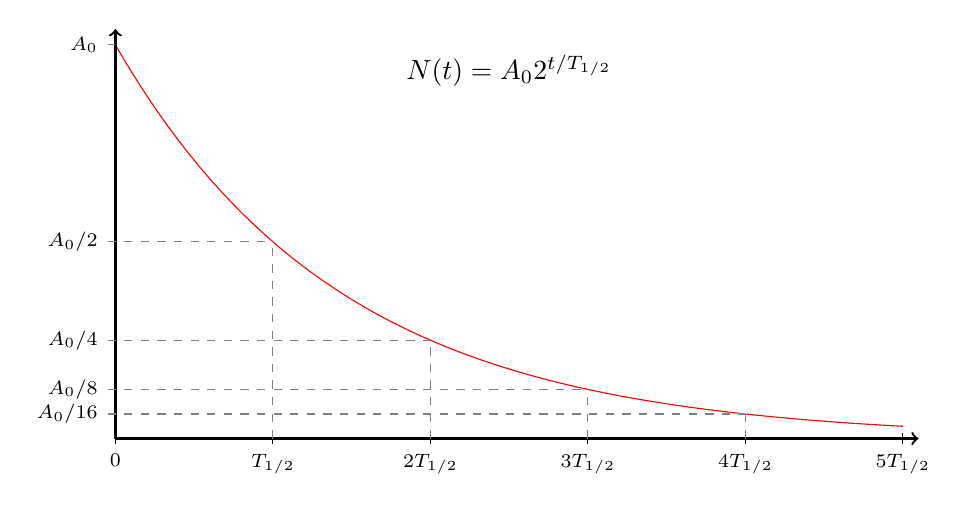
\begin{tikzpicture}
\begin{scope}[]
\clip (0,0) rectangle (10,5);
\begin{scope}[red]
\draw[] (0.0,5.0) -- (0.1,4.829681644624228);
\draw[] (0.1,4.829681644624228) -- (0.2,4.665164957684037);
\draw[] (0.2,4.665164957684037) -- (0.3,4.5062523130541505);
\draw[] (0.3,4.5062523130541505) -- (0.4,4.352752816480621);
\draw[] (0.4,4.352752816480621) -- (0.5,4.204482076268572);
\draw[] (0.5,4.204482076268572) -- (0.6,4.061261981781177);
\draw[] (0.6,4.061261981781177) -- (0.7,3.9229204894837535);
\draw[] (0.7,3.9229204894837535) -- (0.8,3.789291416275995);
\draw[] (0.8,3.789291416275995) -- (0.9,3.6602142398640636);
\draw[] (0.9,3.6602142398640636) -- (1.0,3.5355339059327378);
\draw[] (1.0,3.5355339059327378) -- (1.1,3.4151006418859886);
\draw[] (1.1,3.4151006418859886) -- (1.2,3.2987697769322355);
\draw[] (1.2,3.2987697769322355) -- (1.3,3.1864015682981552);
\draw[] (1.3,3.1864015682981552) -- (1.4,3.0778610333622907);
\draw[] (1.4,3.0778610333622907) -- (1.5,2.9730177875068025);
\draw[] (1.5,2.9730177875068025) -- (1.6,2.871745887492587);
\draw[] (1.6,2.871745887492587) -- (1.7,2.7739236801696125);
\draw[] (1.7,2.7739236801696125) -- (1.8,2.679433656340733);
\draw[] (1.8,2.679433656340733) -- (1.9,2.588162309603444);
\draw[] (1.9,2.588162309603444) -- (2.0,2.5);
\draw[] (2.0,2.5) -- (2.1,2.4148408223121134);
\draw[] (2.1,2.4148408223121134) -- (2.2,2.3325824788420184);
\draw[] (2.2,2.3325824788420184) -- (2.3,2.2531261565270757);
\draw[] (2.3,2.2531261565270757) -- (2.4,2.1763764082403103);
\draw[] (2.4,2.1763764082403103) -- (2.5,2.102241038134286);
\draw[] (2.5,2.102241038134286) -- (2.6,2.0306309908905886);
\draw[] (2.6,2.0306309908905886) -- (2.7,1.9614602447418765);
\draw[] (2.7,1.9614602447418765) -- (2.8,1.8946457081379977);
\draw[] (2.8,1.8946457081379977) -- (2.9,1.8301071199320318);
\draw[] (2.9,1.8301071199320318) -- (3.0,1.7677669529663689);
\draw[] (3.0,1.7677669529663689) -- (3.1,1.7075503209429943);
\draw[] (3.1,1.7075503209429943) -- (3.2,1.6493848884661177);
\draw[] (3.2,1.6493848884661177) -- (3.3,1.5932007841490776);
\draw[] (3.3,1.5932007841490776) -- (3.4,1.5389305166811453);
\draw[] (3.4,1.5389305166811453) -- (3.5,1.4865088937534012);
\draw[] (3.5,1.4865088937534012) -- (3.6,1.4358729437462936);
\draw[] (3.6,1.4358729437462936) -- (3.7,1.386961840084806);
\draw[] (3.7,1.386961840084806) -- (3.8,1.3397168281703664);
\draw[] (3.8,1.3397168281703664) -- (3.9,1.294081154801722);
\draw[] (3.9,1.294081154801722) -- (4.0,1.25);
\draw[] (4.0,1.25) -- (4.1,1.2074204111560571);
\draw[] (4.1,1.2074204111560571) -- (4.2,1.1662912394210092);
\draw[] (4.2,1.1662912394210092) -- (4.3,1.1265630782635379);
\draw[] (4.3,1.1265630782635379) -- (4.4,1.088188204120155);
\draw[] (4.4,1.088188204120155) -- (4.5,1.051120519067143);
\draw[] (4.5,1.051120519067143) -- (4.6,1.0153154954452943);
\draw[] (4.6,1.0153154954452943) -- (4.7,0.9807301223709383);
\draw[] (4.7,0.9807301223709383) -- (4.8,0.9473228540689989);
\draw[] (4.8,0.9473228540689989) -- (4.9,0.9150535599660157);
\draw[] (4.9,0.9150535599660157) -- (5.0,0.8838834764831844);
\draw[] (5.0,0.8838834764831844) -- (5.1,0.8537751604714973);
\draw[] (5.1,0.8537751604714973) -- (5.2,0.8246924442330589);
\draw[] (5.2,0.8246924442330589) -- (5.3,0.7966003920745388);
\draw[] (5.3,0.7966003920745388) -- (5.4,0.7694652583405726);
\draw[] (5.4,0.7694652583405726) -- (5.5,0.7432544468767006);
\draw[] (5.5,0.7432544468767006) -- (5.6,0.7179364718731469);
\draw[] (5.6,0.7179364718731469) -- (5.7,0.693480920042403);
\draw[] (5.7,0.693480920042403) -- (5.8,0.6698584140851832);
\draw[] (5.8,0.6698584140851832) -- (5.9,0.6470405774008609);
\draw[] (5.9,0.6470405774008609) -- (6.0,0.625);
\draw[] (6.0,0.625) -- (6.1,0.6037102055780286);
\draw[] (6.1,0.6037102055780286) -- (6.2,0.5831456197105046);
\draw[] (6.2,0.5831456197105046) -- (6.3,0.5632815391317689);
\draw[] (6.3,0.5632815391317689) -- (6.4,0.5440941020600775);
\draw[] (6.4,0.5440941020600775) -- (6.5,0.5255602595335715);
\draw[] (6.5,0.5255602595335715) -- (6.6,0.5076577477226472);
\draw[] (6.6,0.5076577477226472) -- (6.7,0.49036506118546913);
\draw[] (6.7,0.49036506118546913) -- (6.8,0.4736614270344994);
\draw[] (6.8,0.4736614270344994) -- (6.9,0.45752677998300784);
\draw[] (6.9,0.45752677998300784) -- (7.0,0.4419417382415922);
\draw[] (7.0,0.4419417382415922) -- (7.1,0.42688758023574863);
\draw[] (7.1,0.42688758023574863) -- (7.2,0.41234622211652944);
\draw[] (7.2,0.41234622211652944) -- (7.3,0.3983001960372694);
\draw[] (7.3,0.3983001960372694) -- (7.4,0.3847326291702863);
\draw[] (7.4,0.3847326291702863) -- (7.5,0.3716272234383503);
\draw[] (7.5,0.3716272234383503) -- (7.6,0.35896823593657345);
\draw[] (7.6,0.35896823593657345) -- (7.7,0.3467404600212015);
\draw[] (7.7,0.3467404600212015) -- (7.8,0.3349292070425916);
\draw[] (7.8,0.3349292070425916) -- (7.9,0.3235202887004304);
\draw[] (7.9,0.3235202887004304) -- (8.0,0.3125);
\draw[] (8.0,0.3125) -- (8.1,0.3018551027890143);
\draw[] (8.1,0.3018551027890143) -- (8.2,0.29157280985525236);
\draw[] (8.2,0.29157280985525236) -- (8.3,0.28164076956588435);
\draw[] (8.3,0.28164076956588435) -- (8.4,0.27204705103003873);
\draw[] (8.4,0.27204705103003873) -- (8.5,0.2627801297667858);
\draw[] (8.5,0.2627801297667858) -- (8.6,0.2538288738613236);
\draw[] (8.6,0.2538288738613236) -- (8.7,0.24518253059273465);
\draw[] (8.7,0.24518253059273465) -- (8.8,0.23683071351724963);
\draw[] (8.8,0.23683071351724963) -- (8.9,0.22876338999150392);
\draw[] (8.9,0.22876338999150392) -- (9.0,0.2209708691207961);
\draw[] (9.0,0.2209708691207961) -- (9.1,0.21344379011787432);
\draw[] (9.1,0.21344379011787432) -- (9.2,0.20617311105826477);
\draw[] (9.2,0.20617311105826477) -- (9.3,0.19915009801863465);
\draw[] (9.3,0.19915009801863465) -- (9.4,0.19236631458514314);
\draw[] (9.4,0.19236631458514314) -- (9.5,0.18581361171917515);
\draw[] (9.5,0.18581361171917515) -- (9.6,0.17948411796828673);
\draw[] (9.6,0.17948411796828673) -- (9.7,0.1733702300106008);
\draw[] (9.7,0.1733702300106008) -- (9.8,0.16746460352129575);
\draw[] (9.8,0.16746460352129575) -- (9.9,0.1617601443502152);
\draw[] (9.9,0.1617601443502152) -- (10.0,0.15625);
\end{scope}
\end{scope}
\draw (0,0cm + 2pt) -- (0, 0cm-2pt) node[below] {\scriptsize $0$};
\draw (2,0cm + 2pt) -- (2, 0cm-2pt) node[below] {\scriptsize $T_{1/2}$};
\draw (4,0cm + 2pt) -- (4, 0cm-2pt) node[below] {\scriptsize $2T_{1/2}$};
\draw (6,0cm + 2pt) -- (6, 0cm-2pt) node[below] {\scriptsize $3T_{1/2}$};
\draw (8,0cm + 2pt) -- (8, 0cm-2pt) node[below] {\scriptsize $4T_{1/2}$};
\draw (10,0cm + 2pt) -- (10, 0cm-2pt) node[below] {\scriptsize $5T_{1/2}$};
\node[below] at (5.0,5.0) {$N(t) = A_0 2^{t/T_{1/2}}$};
\draw[thick,->] (0.0,0.0) -- (0.0,5.2);
\draw[thick,->] (0.0,0.0) -- (10.2,0.0);
\draw[thin,gray,dashed] (-0.1,5.0) -- (0.0,5.0);
\node[left] at (-0.1,5.0) {\scriptsize{$A_0$}};
\draw[thin,gray,dashed] (-0.1,2.5) -- (2.0,2.5);
\draw[thin,gray,dashed] (2.0,0.0) -- (2.0,2.5);
\node[left] at (-0.1,2.5) {\scriptsize{$A_0/2$}};
\draw[thin,gray,dashed] (-0.1,1.25) -- (4.0,1.25);
\draw[thin,gray,dashed] (4.0,0.0) -- (4.0,1.25);
\node[left] at (-0.1,1.25) {\scriptsize{$A_0/4$}};
\draw[thin,gray,dashed] (-0.1,0.625) -- (6.0,0.625);
\draw[thin,gray,dashed] (6.0,0.0) -- (6.0,0.625);
\node[left] at (-0.1,0.625) {\scriptsize{$A_0/8$}};
\draw[thin,gray,dashed] (-0.1,0.3125) -- (8.0,0.3125);
\draw[thin,gray,dashed] (8.0,0.0) -- (8.0,0.3125);
\node[left] at (-0.1,0.3125) {\scriptsize{$A_0/16$}};
\end{tikzpicture}
%%% Local Variables: 
%%% mode: latex 
%%% TeX-master: "master" 
%%% End:


  \caption{Graph of radioactive decay.}
\end{figure}

\begin{figure}[H]
  \centering
  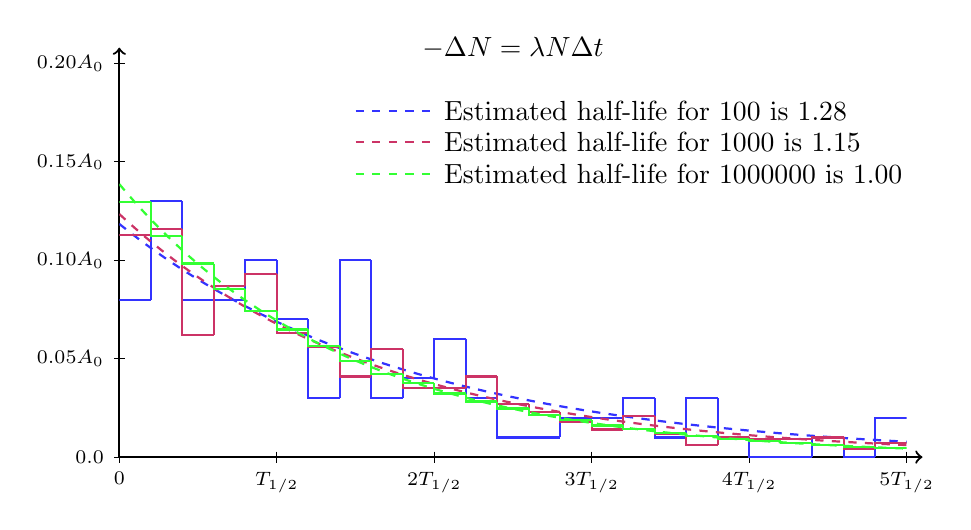
\begin{tikzpicture}
\node[] at (5.0,5.2) {$-\Delta N = \lambda N \Delta t$};
\draw[thick,->] (0.0,0.0) -- (0.0,5.2);
\draw[thick,->] (0.0,0.0) -- (10.2,0.0);
\draw (0,0cm + 2pt) -- (0, 0cm-2pt) node[below] {\scriptsize $0$};
\draw (2,0cm + 2pt) -- (2, 0cm-2pt) node[below] {\scriptsize $T_{1/2}$};
\draw (4,0cm + 2pt) -- (4, 0cm-2pt) node[below] {\scriptsize $2T_{1/2}$};
\draw (6,0cm + 2pt) -- (6, 0cm-2pt) node[below] {\scriptsize $3T_{1/2}$};
\draw (8,0cm + 2pt) -- (8, 0cm-2pt) node[below] {\scriptsize $4T_{1/2}$};
\draw (10,0cm + 2pt) -- (10, 0cm-2pt) node[below] {\scriptsize $5T_{1/2}$};
\draw (0cm+2pt,0.    ) -- (0cm-2pt,0.    ) node[left] {\scriptsize $0.0$};
\draw (0cm+2pt,1.25    ) -- (0cm-2pt,1.25    ) node[left] {\scriptsize $0.05 A_0$};
\draw (0cm+2pt,2.5    ) -- (0cm-2pt,2.5    ) node[left] {\scriptsize $0.10 A_0$};
\draw (0cm+2pt,3.750000093132256    ) -- (0cm-2pt,3.750000093132256    ) node[left] {\scriptsize $0.15 A_0$};
\draw (0cm+2pt,5.    ) -- (0cm-2pt,5.    ) node[left] {\scriptsize $0.20 A_0$};
\begin{scope}[]
\clip (0,0) rectangle (10,5);
\draw[dashed,blue!80,thick] (3.0,4.4) -- (4.0,4.4);
\node[right,] at (4.0,4.4) {Estimated half-life for 100 is  1.28};
\begin{scope}[blue!80,thick]
\draw[] (0.0,1.999999970197678) -- (0.4,1.999999970197678);
\draw (0.4,1.999999970197678) -- (0.4,3.249999951571227) -- (0.8,3.249999951571227);
\draw (0.8,3.249999951571227) -- (0.8,1.999999970197678) -- (1.2,1.999999970197678);
\draw (1.2,1.999999970197678) -- (1.2,1.999999970197678) -- (1.6,1.999999970197678);
\draw (1.6,1.999999970197678) -- (1.6,2.4999999627470975) -- (2.0,2.4999999627470975);
\draw (2.0,2.4999999627470975) -- (2.0,1.7499999739229684) -- (2.4,1.7499999739229684);
\draw (2.4,1.7499999739229684) -- (2.4,0.7499999888241292) -- (2.8,0.7499999888241292);
\draw (2.8,0.7499999888241292) -- (2.8,2.4999999627470975) -- (3.2,2.4999999627470975);
\draw (3.2,2.4999999627470975) -- (3.2,0.7499999888241292) -- (3.6000001,0.7499999888241292);
\draw (3.6000001,0.7499999888241292) -- (3.6000001,0.999999985098839) -- (4.0,0.999999985098839);
\draw (4.0,0.999999985098839) -- (4.0,1.4999999776482584) -- (4.4,1.4999999776482584);
\draw (4.4,1.4999999776482584) -- (4.4,0.7499999888241292) -- (4.8,0.7499999888241292);
\draw (4.8,0.7499999888241292) -- (4.8,0.24999999627470976) -- (5.2000003,0.24999999627470976);
\draw (5.2000003,0.24999999627470976) -- (5.2000003,0.24999999627470976) -- (5.6,0.24999999627470976);
\draw (5.6,0.24999999627470976) -- (5.6,0.4999999925494195) -- (6.0,0.4999999925494195);
\draw (6.0,0.4999999925494195) -- (6.0,0.4999999925494195) -- (6.4,0.4999999925494195);
\draw (6.4,0.4999999925494195) -- (6.4,0.7499999888241292) -- (6.8,0.7499999888241292);
\draw (6.8,0.7499999888241292) -- (6.8,0.24999999627470976) -- (7.2000003,0.24999999627470976);
\draw (7.2000003,0.24999999627470976) -- (7.2000003,0.7499999888241292) -- (7.6,0.7499999888241292);
\draw (7.6,0.7499999888241292) -- (7.6,0.24999999627470976) -- (8.0,0.24999999627470976);
\draw (8.0,0.24999999627470976) -- (8.0,0.0) -- (8.400001,0.0);
\draw (8.400001,0.0) -- (8.400001,0.0) -- (8.8,0.0);
\draw (8.8,0.0) -- (8.8,0.24999999627470976) -- (9.2,0.24999999627470976);
\draw (9.2,0.24999999627470976) -- (9.2,0.0) -- (9.6,0.0);
\draw (9.6,0.0) -- (9.6,0.4999999925494195) -- (10.0,0.4999999925494195);
\end{scope}
\begin{scope}[dashed,blue!80,thick]
\pgfpathmoveto{ \pgfqpoint {0.0cm} {2.961035269001679cm}}
\pgfpathlineto{ \pgfqpoint {0.1cm} {2.8816374412713213cm}}
\pgfpathlineto{ \pgfqpoint {0.2cm} {2.8043686037337845cm}}
\pgfpathlineto{ \pgfqpoint {0.3cm} {2.7291716691944843cm}}
\pgfpathlineto{ \pgfqpoint {0.4cm} {2.6559910812069814cm}}
\pgfpathlineto{ \pgfqpoint {0.5cm} {2.5847727730271752cm}}
\pgfpathlineto{ \pgfqpoint {0.6cm} {2.515464127668107cm}}
\pgfpathlineto{ \pgfqpoint {0.7cm} {2.448013939025868cm}}
\pgfpathlineto{ \pgfqpoint {0.8cm} {2.382372374047879cm}}
\pgfpathlineto{ \pgfqpoint {0.9cm} {2.318490935915604cm}}
\pgfpathlineto{ \pgfqpoint {1.0cm} {2.2563224282144825cm}}
\pgfpathlineto{ \pgfqpoint {1.1cm} {2.1958209200646266cm}}
\pgfpathlineto{ \pgfqpoint {1.2cm} {2.136941712186503cm}}
\pgfpathlineto{ \pgfqpoint {1.3cm} {2.0796413038765396cm}}
\pgfpathlineto{ \pgfqpoint {1.4cm} {2.0238773608682563cm}}
\pgfpathlineto{ \pgfqpoint {1.5cm} {1.9696086840551748cm}}
\pgfpathlineto{ \pgfqpoint {1.6cm} {1.9167951790523947cm}}
\pgfpathlineto{ \pgfqpoint {1.7cm} {1.8653978265743565cm}}
\pgfpathlineto{ \pgfqpoint {1.8cm} {1.8153786536069cm}}
\pgfpathlineto{ \pgfqpoint {1.9cm} {1.7667007053523203cm}}
\pgfpathlineto{ \pgfqpoint {2.0cm} {1.7193280179266968cm}}
\pgfpathlineto{ \pgfqpoint {2.1cm} {1.6732255917893186cm}}
\pgfpathlineto{ \pgfqpoint {2.2cm} {1.6283593658845843cm}}
\pgfpathlineto{ \pgfqpoint {2.3cm} {1.5846961924772622cm}}
\pgfpathlineto{ \pgfqpoint {2.4cm} {1.5422038126625208cm}}
\pgfpathlineto{ \pgfqpoint {2.5cm} {1.5008508325326482cm}}
\pgfpathlineto{ \pgfqpoint {2.6cm} {1.4606066999828298cm}}
\pgfpathlineto{ \pgfqpoint {2.7cm} {1.4214416821388707cm}}
\pgfpathlineto{ \pgfqpoint {2.8cm} {1.383326843390171cm}}
\pgfpathlineto{ \pgfqpoint {2.9cm} {1.3462340240117303cm}}
\pgfpathlineto{ \pgfqpoint {3.0cm} {1.3101358193593868cm}}
\pgfpathlineto{ \pgfqpoint {3.1cm} {1.2750055596229204cm}}
\pgfpathlineto{ \pgfqpoint {3.2cm} {1.2408172901220575cm}}
\pgfpathlineto{ \pgfqpoint {3.3cm} {1.207545752130828cm}}
\pgfpathlineto{ \pgfqpoint {3.4cm} {1.175166364216096cm}}
\pgfpathlineto{ \pgfqpoint {3.5cm} {1.1436552040764874cm}}
\pgfpathlineto{ \pgfqpoint {3.6cm} {1.1129889908682922cm}}
\pgfpathlineto{ \pgfqpoint {3.7cm} {1.0831450680052797cm}}
\pgfpathlineto{ \pgfqpoint {3.8cm} {1.0541013864197295cm}}
\pgfpathlineto{ \pgfqpoint {3.9cm} {1.0258364882722981cm}}
\pgfpathlineto{ \pgfqpoint {4.0cm} {0.9983294910986982cm}}
\pgfpathlineto{ \pgfqpoint {4.1cm} {0.9715600723814687cm}}
\pgfpathlineto{ \pgfqpoint {4.2cm} {0.9455084545354424cm}}
\pgfpathlineto{ \pgfqpoint {4.3cm} {0.9201553902958152cm}}
\pgfpathlineto{ \pgfqpoint {4.4cm} {0.8954821484980237cm}}
\pgfpathlineto{ \pgfqpoint {4.5cm} {0.8714705002389241cm}}
\pgfpathlineto{ \pgfqpoint {4.6cm} {0.848102705409048cm}}
\pgfpathlineto{ \pgfqpoint {4.7cm} {0.8253614995859841cm}}
\pgfpathlineto{ \pgfqpoint {4.8cm} {0.8032300812792068cm}}
\pgfpathlineto{ \pgfqpoint {4.9cm} {0.7816920995169194cm}}
\pgfpathlineto{ \pgfqpoint {5.0cm} {0.7607316417657523cm}}
\pgfpathlineto{ \pgfqpoint {5.1cm} {0.7403332221743797cm}}
\pgfpathlineto{ \pgfqpoint {5.2cm} {0.7204817701323781cm}}
\pgfpathlineto{ \pgfqpoint {5.3cm} {0.7011626191358686cm}}
\pgfpathlineto{ \pgfqpoint {5.4cm} {0.6823614959517176cm}}
\pgfpathlineto{ \pgfqpoint {5.5cm} {0.6640645100722925cm}}
\pgfpathlineto{ \pgfqpoint {5.6cm} {0.6462581434529782cm}}
\pgfpathlineto{ \pgfqpoint {5.7cm} {0.6289292405248749cm}}
\pgfpathlineto{ \pgfqpoint {5.8cm} {0.612064998475298cm}}
\pgfpathlineto{ \pgfqpoint {5.9cm} {0.595652957788897cm}}
\pgfpathlineto{ \pgfqpoint {6.0cm} {0.5796809930424096cm}}
\pgfpathlineto{ \pgfqpoint {6.1cm} {0.5641373039462438cm}}
\pgfpathlineto{ \pgfqpoint {6.2cm} {0.5490104066262759cm}}
\pgfpathlineto{ \pgfqpoint {6.3cm} {0.5342891251394184cm}}
\pgfpathlineto{ \pgfqpoint {6.4cm} {0.5199625832166923cm}}
\pgfpathlineto{ \pgfqpoint {6.5cm} {0.506020196227702cm}}
\pgfpathlineto{ \pgfqpoint {6.6cm} {0.4924516633605759cm}}
\pgfpathlineto{ \pgfqpoint {6.7cm} {0.47924696001159706cm}}
\pgfpathlineto{ \pgfqpoint {6.8cm} {0.46639633037889855cm}}
\pgfpathlineto{ \pgfqpoint {6.9cm} {0.45389028025475403cm}}
\pgfpathlineto{ \pgfqpoint {7.0cm} {0.4417195700111368cm}}
\pgfpathlineto{ \pgfqpoint {7.1cm} {0.4298752077733657cm}}
\pgfpathlineto{ \pgfqpoint {7.2cm} {0.4183484427767946cm}}
\pgfpathlineto{ \pgfqpoint {7.3cm} {0.40713075890163625cm}}
\pgfpathlineto{ \pgfqpoint {7.4cm} {0.3962138683811458cm}}
\pgfpathlineto{ \pgfqpoint {7.5cm} {0.38558970567851414cm}}
\pgfpathlineto{ \pgfqpoint {7.6cm} {0.37525042152794624cm}}
\pgfpathlineto{ \pgfqpoint {7.7cm} {0.3651883771355249cm}}
\pgfpathlineto{ \pgfqpoint {7.8cm} {0.3553961385355737cm}}
\pgfpathlineto{ \pgfqpoint {7.9cm} {0.3458664710983481cm}}
\pgfpathlineto{ \pgfqpoint {8.0cm} {0.3365923341850003cm}}
\pgfpathlineto{ \pgfqpoint {8.1cm} {0.3275668759458656cm}}
\pgfpathlineto{ \pgfqpoint {8.2cm} {0.3187834282582297cm}}
\pgfpathlineto{ \pgfqpoint {8.3cm} {0.3102355017998348cm}}
\pgfpathlineto{ \pgfqpoint {8.4cm} {0.30191678125448684cm}}
\pgfpathlineto{ \pgfqpoint {8.5cm} {0.29382112064621935cm}}
\pgfpathlineto{ \pgfqpoint {8.6cm} {0.285942538798569cm}}
\pgfpathlineto{ \pgfqpoint {8.7cm} {0.27827521491560686cm}}
\pgfpathlineto{ \pgfqpoint {8.8cm} {0.2708134842814604cm}}
\pgfpathlineto{ \pgfqpoint {8.9cm} {0.2635518340751504cm}}
\pgfpathlineto{ \pgfqpoint {9.0cm} {0.2564848992976483cm}}
\pgfpathlineto{ \pgfqpoint {9.1cm} {0.24960745880814725cm}}
\pgfpathlineto{ \pgfqpoint {9.2cm} {0.2429144314666177cm}}
\pgfpathlineto{ \pgfqpoint {9.3cm} {0.23640087237979632cm}}
\pgfpathlineto{ \pgfqpoint {9.4cm} {0.23006196924783684cm}}
\pgfpathlineto{ \pgfqpoint {9.5cm} {0.22389303880892142cm}}
\pgfpathlineto{ \pgfqpoint {9.6cm} {0.2178895233792081cm}}
\pgfpathlineto{ \pgfqpoint {9.7cm} {0.212046987485556cm}}
\pgfpathlineto{ \pgfqpoint {9.8cm} {0.2063611145885419cm}}
\pgfpathlineto{ \pgfqpoint {9.9cm} {0.20082770389334617cm}}
\pgfpathlineto{ \pgfqpoint {10.0cm} {0.1954426672461525cm}}
\pgfusepath{ stroke }
\end{scope}
\draw[dashed,purple!80,thick] (3.0,4.0) -- (4.0,4.0);
\node[right,] at (4.0,4.0) {Estimated half-life for 1000 is  1.15};
\begin{scope}[purple!80,thick]
\draw[] (0.0,2.8249999579042204) -- (0.4,2.8249999579042204);
\draw (0.4,2.8249999579042204) -- (0.4,2.8999999567866332) -- (0.8,2.8999999567866332);
\draw (0.8,2.8999999567866332) -- (0.8,1.5499999769032005) -- (1.2,1.5499999769032005);
\draw (1.2,1.5499999769032005) -- (1.2,2.1749999675899745) -- (1.6,2.1749999675899745);
\draw (1.6,2.1749999675899745) -- (1.6,2.3249999653548006) -- (2.0,2.3249999653548006);
\draw (2.0,2.3249999653548006) -- (2.0,1.5749999765306715) -- (2.4,1.5749999765306715);
\draw (2.4,1.5749999765306715) -- (2.4,1.3999999791383746) -- (2.8,1.3999999791383746);
\draw (2.8,1.3999999791383746) -- (2.8,1.02499998472631) -- (3.2,1.02499998472631);
\draw (3.2,1.02499998472631) -- (3.2,1.3749999795109036) -- (3.6000001,1.3749999795109036);
\draw (3.6000001,1.3749999795109036) -- (3.6000001,0.8749999869614842) -- (4.0,0.8749999869614842);
\draw (4.0,0.8749999869614842) -- (4.0,0.8749999869614842) -- (4.4,0.8749999869614842);
\draw (4.4,0.8749999869614842) -- (4.4,1.02499998472631) -- (4.8,1.02499998472631);
\draw (4.8,1.02499998472631) -- (4.8,0.6749999899417163) -- (5.2000003,0.6749999899417163);
\draw (5.2000003,0.6749999899417163) -- (5.2000003,0.5749999914318324) -- (5.6,0.5749999914318324);
\draw (5.6,0.5749999914318324) -- (5.6,0.44999999329447754) -- (6.0,0.44999999329447754);
\draw (6.0,0.44999999329447754) -- (6.0,0.34999999478459365) -- (6.4,0.34999999478459365);
\draw (6.4,0.34999999478459365) -- (6.4,0.5249999921768905) -- (6.8,0.5249999921768905);
\draw (6.8,0.5249999921768905) -- (6.8,0.29999999552965173) -- (7.2000003,0.29999999552965173);
\draw (7.2000003,0.29999999552965173) -- (7.2000003,0.14999999776482587) -- (7.6,0.14999999776482587);
\draw (7.6,0.14999999776482587) -- (7.6,0.24999999627470976) -- (8.0,0.24999999627470976);
\draw (8.0,0.24999999627470976) -- (8.0,0.22499999664723877) -- (8.400001,0.22499999664723877);
\draw (8.400001,0.22499999664723877) -- (8.400001,0.22499999664723877) -- (8.8,0.22499999664723877);
\draw (8.8,0.22499999664723877) -- (8.8,0.24999999627470976) -- (9.2,0.24999999627470976);
\draw (9.2,0.24999999627470976) -- (9.2,0.0999999985098839) -- (9.6,0.0999999985098839);
\draw (9.6,0.0999999985098839) -- (9.6,0.17499999739229682) -- (10.0,0.17499999739229682);
\end{scope}
\begin{scope}[dashed,purple!80,thick]
\pgfpathmoveto{ \pgfqpoint {0.0cm} {3.086841841736368cm}}
\pgfpathlineto{ \pgfqpoint {0.1cm} {2.9954103434620447cm}}
\pgfpathlineto{ \pgfqpoint {0.2cm} {2.9066870237421454cm}}
\pgfpathlineto{ \pgfqpoint {0.3cm} {2.820591666992095cm}}
\pgfpathlineto{ \pgfqpoint {0.4cm} {2.7370464335932585cm}}
\pgfpathlineto{ \pgfqpoint {0.5cm} {2.6559757895174174cm}}
\pgfpathlineto{ \pgfqpoint {0.6cm} {2.5773064380357407cm}}
\pgfpathlineto{ \pgfqpoint {0.7cm} {2.5009672534505296cm}}
\pgfpathlineto{ \pgfqpoint {0.8cm} {2.4268892167898066cm}}
\pgfpathlineto{ \pgfqpoint {0.9cm} {2.355005353406617cm}}
\pgfpathlineto{ \pgfqpoint {1.0cm} {2.2852506724266233cm}}
\pgfpathlineto{ \pgfqpoint {1.1cm} {2.217562107989244cm}}
\pgfpathlineto{ \pgfqpoint {1.2cm} {2.1518784622292233cm}}
\pgfpathlineto{ \pgfqpoint {1.3cm} {2.0881403499470625cm}}
\pgfpathlineto{ \pgfqpoint {1.4cm} {2.0262901449183093cm}}
\pgfpathlineto{ \pgfqpoint {1.5cm} {1.9662719277931449cm}}
\pgfpathlineto{ \pgfqpoint {1.6cm} {1.9080314355391774cm}}
\pgfpathlineto{ \pgfqpoint {1.7cm} {1.8515160123817274cm}}
\pgfpathlineto{ \pgfqpoint {1.8cm} {1.796674562197245cm}}
\pgfpathlineto{ \pgfqpoint {1.9cm} {1.7434575023168293cm}}
\pgfpathlineto{ \pgfqpoint {2.0cm} {1.691816718698071cm}}
\pgfpathlineto{ \pgfqpoint {2.1cm} {1.6417055224246973cm}}
\pgfpathlineto{ \pgfqpoint {2.2cm} {1.593078607494684cm}}
\pgfpathlineto{ \pgfqpoint {2.3cm} {1.5458920098586757cm}}
\pgfpathlineto{ \pgfqpoint {2.4cm} {1.5001030676716742cm}}
\pgfpathlineto{ \pgfqpoint {2.5cm} {1.4556703827220696cm}}
\pgfpathlineto{ \pgfqpoint {2.6cm} {1.4125537830031254cm}}
\pgfpathlineto{ \pgfqpoint {2.7cm} {1.3707142863930917cm}}
\pgfpathlineto{ \pgfqpoint {2.8cm} {1.3301140654111052cm}}
\pgfpathlineto{ \pgfqpoint {2.9cm} {1.2907164130170066cm}}
\pgfpathlineto{ \pgfqpoint {3.0cm} {1.2524857094241648cm}}
\pgfpathlineto{ \pgfqpoint {3.1cm} {1.2153873898952923cm}}
\pgfpathlineto{ \pgfqpoint {3.2cm} {1.179387913492142cm}}
\pgfpathlineto{ \pgfqpoint {3.3cm} {1.1444547327508323cm}}
\pgfpathlineto{ \pgfqpoint {3.4cm} {1.1105562642553786cm}}
\pgfpathlineto{ \pgfqpoint {3.5cm} {1.077661860082832cm}}
\pgfpathlineto{ \pgfqpoint {3.6cm} {1.0457417800942046cm}}
\pgfpathlineto{ \pgfqpoint {3.7cm} {1.014767165046131cm}}
\pgfpathlineto{ \pgfqpoint {3.8cm} {0.9847100104989565cm}}
\pgfpathlineto{ \pgfqpoint {3.9cm} {0.9555431414976606cm}}
\pgfpathlineto{ \pgfqpoint {4.0cm} {0.9272401880027255cm}}
\pgfpathlineto{ \pgfqpoint {4.1cm} {0.8997755610487362cm}}
\pgfpathlineto{ \pgfqpoint {4.2cm} {0.8731244296091581cm}}
\pgfpathlineto{ \pgfqpoint {4.3cm} {0.8472626981463717cm}}
\pgfpathlineto{ \pgfqpoint {4.4cm} {0.8221669848266726cm}}
\pgfpathlineto{ \pgfqpoint {4.5cm} {0.7978146003805356cm}}
\pgfpathlineto{ \pgfqpoint {4.6cm} {0.7741835275890351cm}}
\pgfpathlineto{ \pgfqpoint {4.7cm} {0.7512524013778684cm}}
\pgfpathlineto{ \pgfqpoint {4.8cm} {0.7290004895009958cm}}
\pgfpathlineto{ \pgfqpoint {4.9cm} {0.7074076737964186cm}}
\pgfpathlineto{ \pgfqpoint {5.0cm} {0.6864544319971635cm}}
\pgfpathlineto{ \pgfqpoint {5.1cm} {0.6661218200810166cm}}
\pgfpathlineto{ \pgfqpoint {5.2cm} {0.6463914551430555cm}}
\pgfpathlineto{ \pgfqpoint {5.3cm} {0.6272454987754936cm}}
\pgfpathlineto{ \pgfqpoint {5.4cm} {0.608666640939807cm}}
\pgfpathlineto{ \pgfqpoint {5.5cm} {0.5906380843165687cm}}
\pgfpathlineto{ \pgfqpoint {5.6cm} {0.5731435291188322cm}}
\pgfpathlineto{ \pgfqpoint {5.7cm} {0.556167158355343cm}}
\pgfpathlineto{ \pgfqpoint {5.8cm} {0.539693623530249cm}}
\pgfpathlineto{ \pgfqpoint {5.9cm} {0.52370803076638cm}}
\pgfpathlineto{ \pgfqpoint {6.0cm} {0.5081959273395551cm}}
\pgfpathlineto{ \pgfqpoint {6.1cm} {0.4931432886117389cm}}
\pgfpathlineto{ \pgfqpoint {6.2cm} {0.4785365053512349cm}}
\pgfpathlineto{ \pgfqpoint {6.3cm} {0.4643623714284517cm}}
\pgfpathlineto{ \pgfqpoint {6.4cm} {0.45060807187611746cm}}
\pgfpathlineto{ \pgfqpoint {6.5cm} {0.437261171303148cm}}
\pgfpathlineto{ \pgfqpoint {6.6cm} {0.4243096026516932cm}}
\pgfpathlineto{ \pgfqpoint {6.7cm} {0.4117416562871964cm}}
\pgfpathlineto{ \pgfqpoint {6.8cm} {0.39954596941160536cm}}
\pgfpathlineto{ \pgfqpoint {6.9cm} {0.3877115157901588cm}}
\pgfpathlineto{ \pgfqpoint {7.0cm} {0.37622759578246484cm}}
\pgfpathlineto{ \pgfqpoint {7.1cm} {0.3650838266688561cm}}
\pgfpathlineto{ \pgfqpoint {7.2cm} {0.3542701332632748cm}}
\pgfpathlineto{ \pgfqpoint {7.3cm} {0.3437767388042038cm}}
\pgfpathlineto{ \pgfqpoint {7.4cm} {0.3335941561154035cm}}
\pgfpathlineto{ \pgfqpoint {7.5cm} {0.32371317902846836cm}}
\pgfpathlineto{ \pgfqpoint {7.6cm} {0.3141248740594428cm}}
\pgfpathlineto{ \pgfqpoint {7.7cm} {0.30482057233197496cm}}
\pgfpathlineto{ \pgfqpoint {7.8cm} {0.29579186173970434cm}}
\pgfpathlineto{ \pgfqpoint {7.9cm} {0.28703057934079795cm}}
\pgfpathlineto{ \pgfqpoint {8.0cm} {0.2785288039777578cm}}
\pgfpathlineto{ \pgfqpoint {8.1cm} {0.27027884911582795cm}}
\pgfpathlineto{ \pgfqpoint {8.2cm} {0.2622732558935269cm}}
\pgfpathlineto{ \pgfqpoint {8.3cm} {0.254504786379021cm}}
\pgfpathlineto{ \pgfqpoint {8.4cm} {0.24696641702624234cm}}
\pgfpathlineto{ \pgfqpoint {8.5cm} {0.2396513323248347cm}}
\pgfpathlineto{ \pgfqpoint {8.6cm} {0.23255291863818733cm}}
\pgfpathlineto{ \pgfqpoint {8.7cm} {0.22566475822398363cm}}
\pgfpathlineto{ \pgfqpoint {8.8cm} {0.21898062343186042cm}}
\pgfpathlineto{ \pgfqpoint {8.9cm} {0.21249447107293098cm}}
\pgfpathlineto{ \pgfqpoint {9.0cm} {0.2062004369560813cm}}
\pgfpathlineto{ \pgfqpoint {9.1cm} {0.20009283058609992cm}}
\pgfpathlineto{ \pgfqpoint {9.2cm} {0.19416613001884753cm}}
\pgfpathlineto{ \pgfqpoint {9.3cm} {0.18841497686881623cm}}
\pgfpathlineto{ \pgfqpoint {9.4cm} {0.18283417146456282cm}}
\pgfpathlineto{ \pgfqpoint {9.5cm} {0.17741866814763682cm}}
\pgfpathlineto{ \pgfqpoint {9.6cm} {0.17216357071075347cm}}
\pgfpathlineto{ \pgfqpoint {9.7cm} {0.16706412797108683cm}}
\pgfpathlineto{ \pgfqpoint {9.8cm} {0.16211572947468136cm}}
\pgfpathlineto{ \pgfqpoint {9.9cm} {0.15731390132809664cm}}
\pgfpathlineto{ \pgfqpoint {10.0cm} {0.15265430215351894cm}}
\pgfusepath{ stroke }
\end{scope}
\draw[dashed,green!80,thick] (3.0,3.6) -- (4.0,3.6);
\node[right,] at (4.0,3.6) {Estimated half-life for 1000000 is  1.00};
\begin{scope}[green!80,thick]
\draw[] (0.0,3.24324995167181) -- (0.4,3.24324995167181);
\draw (0.4,3.24324995167181) -- (0.4,2.803499958224595) -- (0.8,2.803499958224595);
\draw (0.8,2.803499958224595) -- (0.8,2.4576499633781617) -- (1.2,2.4576499633781617);
\draw (1.2,2.4576499633781617) -- (1.2,2.1366749681610617) -- (1.6,2.1366749681610617);
\draw (1.6,2.1366749681610617) -- (1.6,1.8505749724242841) -- (2.0,1.8505749724242841);
\draw (2.0,1.8505749724242841) -- (2.0,1.6215999758362774) -- (2.4,1.6215999758362774);
\draw (2.4,1.6215999758362774) -- (2.4,1.412174978956953) -- (2.8,1.412174978956953);
\draw (2.8,1.412174978956953) -- (2.8,1.2185999818414452) -- (3.2,1.2185999818414452);
\draw (3.2,1.2185999818414452) -- (3.2,1.0593749842140827) -- (3.6000001,1.0593749842140827);
\draw (3.6000001,1.0593749842140827) -- (3.6000001,0.9370249860372396) -- (4.0,0.9370249860372396);
\draw (4.0,0.9370249860372396) -- (4.0,0.8068999879762532) -- (4.4,0.8068999879762532);
\draw (4.4,0.8068999879762532) -- (4.4,0.7056249894853682) -- (4.8,0.7056249894853682);
\draw (4.8,0.7056249894853682) -- (4.8,0.6178499907933177) -- (5.2000003,0.6178499907933177);
\draw (5.2000003,0.6178499907933177) -- (5.2000003,0.5375749919895084) -- (5.6,0.5375749919895084);
\draw (5.6,0.5375749919895084) -- (5.6,0.46742499303482477) -- (6.0,0.46742499303482477);
\draw (6.0,0.46742499303482477) -- (6.0,0.4023249940048904) -- (6.4,0.4023249940048904);
\draw (6.4,0.4023249940048904) -- (6.4,0.3524499947480858) -- (6.8,0.3524499947480858);
\draw (6.8,0.3524499947480858) -- (6.8,0.30812499540857974) -- (7.2000003,0.30812499540857974);
\draw (7.2000003,0.30812499540857974) -- (7.2000003,0.2634999960735441) -- (7.6,0.2634999960735441);
\draw (7.6,0.2634999960735441) -- (7.6,0.23042499656639998) -- (8.0,0.23042499656639998);
\draw (8.0,0.23042499656639998) -- (8.0,0.20917499688304964) -- (8.400001,0.20917499688304964);
\draw (8.400001,0.20917499688304964) -- (8.400001,0.17444999740049247) -- (8.8,0.17444999740049247);
\draw (8.8,0.17444999740049247) -- (8.8,0.1550249976899475) -- (9.2,0.1550249976899475);
\draw (9.2,0.1550249976899475) -- (9.2,0.1326249980237335) -- (9.6,0.1326249980237335);
\draw (9.6,0.1326249980237335) -- (9.6,0.11359999830722811) -- (10.0,0.11359999830722811);
\end{scope}
\begin{scope}[dashed,green!80,thick]
\pgfpathmoveto{ \pgfqpoint {0.0cm} {3.467170414395642cm}}
\pgfpathlineto{ \pgfqpoint {0.1cm} {3.349093928616908cm}}
\pgfpathlineto{ \pgfqpoint {0.2cm} {3.2350386055811327cm}}
\pgfpathlineto{ \pgfqpoint {0.3cm} {3.1248675022746526cm}}
\pgfpathlineto{ \pgfqpoint {0.4cm} {3.018448339357021cm}}
\pgfpathlineto{ \pgfqpoint {0.5cm} {2.915653342336934cm}}
\pgfpathlineto{ \pgfqpoint {0.6cm} {2.8163590881569953cm}}
\pgfpathlineto{ \pgfqpoint {0.7cm} {2.7204463570031265cm}}
\pgfpathlineto{ \pgfqpoint {0.8cm} {2.627799989160697cm}}
\pgfpathlineto{ \pgfqpoint {0.9cm} {2.538308746745497cm}}
\pgfpathlineto{ \pgfqpoint {1.0cm} {2.451865180143544cm}}
\pgfpathlineto{ \pgfqpoint {1.1cm} {2.3683654989993577cm}}
\pgfpathlineto{ \pgfqpoint {1.2cm} {2.287709447597804cm}}
\pgfpathlineto{ \pgfqpoint {1.3cm} {2.2098001844898802cm}}
\pgfpathlineto{ \pgfqpoint {1.4cm} {2.134544166217919cm}}
\pgfpathlineto{ \pgfqpoint {1.5cm} {2.061851035000588cm}}
\pgfpathlineto{ \pgfqpoint {1.6cm} {1.9916335102428526cm}}
\pgfpathlineto{ \pgfqpoint {1.7cm} {1.9238072837406195cm}}
\pgfpathlineto{ \pgfqpoint {1.8cm} {1.8582909184542544cm}}
\pgfpathlineto{ \pgfqpoint {1.9cm} {1.795005750729419cm}}
\pgfpathlineto{ \pgfqpoint {2.0cm} {1.733875795847841cm}}
\pgfpathlineto{ \pgfqpoint {2.1cm} {1.6748276567945994cm}}
\pgfpathlineto{ \pgfqpoint {2.2cm} {1.6177904361323991cm}}
\pgfpathlineto{ \pgfqpoint {2.3cm} {1.5626956508770122cm}}
\pgfpathlineto{ \pgfqpoint {2.4cm} {1.5094771502716904cm}}
\pgfpathlineto{ \pgfqpoint {2.5cm} {1.4580710363618128cm}}
\pgfpathlineto{ \pgfqpoint {2.6cm} {1.4084155872744135cm}}
\pgfpathlineto{ \pgfqpoint {2.7cm} {1.3604511831104658cm}}
\pgfpathlineto{ \pgfqpoint {2.8cm} {1.3141202343609497cm}}
\pgfpathlineto{ \pgfqpoint {2.9cm} {1.2693671127607487cm}}
\pgfpathlineto{ \pgfqpoint {3.0cm} {1.2261380844973617cm}}
\pgfpathlineto{ \pgfqpoint {3.1cm} {1.184381245694227cm}}
\pgfpathlineto{ \pgfqpoint {3.2cm} {1.1440464600911981cm}}
\pgfpathlineto{ \pgfqpoint {3.3cm} {1.1050852988473499cm}}
\pgfpathlineto{ \pgfqpoint {3.4cm} {1.067450982393833cm}}
\pgfpathlineto{ \pgfqpoint {3.5cm} {1.0310983242669634cm}}
\pgfpathlineto{ \pgfqpoint {3.6cm} {0.9959836768541087cm}}
\pgfpathlineto{ \pgfqpoint {3.7cm} {0.9620648789872278cm}}
\pgfpathlineto{ \pgfqpoint {3.8cm} {0.9293012053211455cm}}
\pgfpathlineto{ \pgfqpoint {3.9cm} {0.8976533174357761cm}}
\pgfpathlineto{ \pgfqpoint {4.0cm} {0.8670832166035926cm}}
\pgfpathlineto{ \pgfqpoint {4.1cm} {0.8375541981656225cm}}
\pgfpathlineto{ \pgfqpoint {4.2cm} {0.8090308074611997cm}}
\pgfpathlineto{ \pgfqpoint {4.3cm} {0.7814787972585514cm}}
\pgfpathlineto{ \pgfqpoint {4.4cm} {0.7548650866351102cm}}
\pgfpathlineto{ \pgfqpoint {4.5cm} {0.7291577212581852cm}}
\pgfpathlineto{ \pgfqpoint {4.6cm} {0.7043258350182924cm}}
\pgfpathlineto{ \pgfqpoint {4.7cm} {0.6803396129690857cm}}
\pgfpathlineto{ \pgfqpoint {4.8cm} {0.657170255529395cm}}
\pgfpathlineto{ \pgfqpoint {4.9cm} {0.634789943904375cm}}
\pgfpathlineto{ \pgfqpoint {5.0cm} {0.6131718066842659cm}}
\pgfpathlineto{ \pgfqpoint {5.1cm} {0.5922898875806458cm}}
\pgfpathlineto{ \pgfqpoint {5.2cm} {0.5721191142614477cm}}
\pgfpathlineto{ \pgfqpoint {5.3cm} {0.5526352682473172cm}}
\pgfpathlineto{ \pgfqpoint {5.4cm} {0.5338149558331651cm}}
\pgfpathlineto{ \pgfqpoint {5.5cm} {0.5156355800000055cm}}
\pgfpathlineto{ \pgfqpoint {5.6cm} {0.4980753132833515cm}}
\pgfpathlineto{ \pgfqpoint {5.7cm} {0.48111307156559274cm}}
\pgfpathlineto{ \pgfqpoint {5.8cm} {0.464728488760891cm}}
\pgfpathlineto{ \pgfqpoint {5.9cm} {0.44890189236219247cm}}
\pgfpathlineto{ \pgfqpoint {6.0cm} {0.4336142798210044cm}}
\pgfpathlineto{ \pgfqpoint {6.1cm} {0.41884729573156937cm}}
\pgfpathlineto{ \pgfqpoint {6.2cm} {0.4045832097920466cm}}
\pgfpathlineto{ \pgfqpoint {6.3cm} {0.3908048955162391cm}}
\pgfpathlineto{ \pgfqpoint {6.4cm} {0.37749580967030255cm}}
\pgfpathlineto{ \pgfqpoint {6.5cm} {0.36463997240975166cm}}
\pgfpathlineto{ \pgfqpoint {6.6cm} {0.3522219480929104cm}}
\pgfpathlineto{ \pgfqpoint {6.7cm} {0.3402268267477717cm}}
\pgfpathlineto{ \pgfqpoint {6.8cm} {0.3286402061700146cm}}
\pgfpathlineto{ \pgfqpoint {6.9cm} {0.31744817463068287cm}}
\pgfpathlineto{ \pgfqpoint {7.0cm} {0.3066372941727638cm}}
\pgfpathlineto{ \pgfqpoint {7.1cm} {0.2961945844766122cm}}
\pgfpathlineto{ \pgfqpoint {7.2cm} {0.28610750727484535cm}}
\pgfpathlineto{ \pgfqpoint {7.3cm} {0.27636395129799957cm}}
\pgfpathlineto{ \pgfqpoint {7.4cm} {0.26695221773286965cm}}
\pgfpathlineto{ \pgfqpoint {7.5cm} {0.25786100617607316cm}}
\pgfpathlineto{ \pgfqpoint {7.6cm} {0.24907940106597465cm}}
\pgfpathlineto{ \pgfqpoint {7.7cm} {0.24059685857667834cm}}
\pgfpathlineto{ \pgfqpoint {7.8cm} {0.23240319395835315cm}}
\pgfpathlineto{ \pgfqpoint {7.9cm} {0.22448856930869082cm}}
\pgfpathlineto{ \pgfqpoint {8.0cm} {0.2168434817608132cm}}
\pgfpathlineto{ \pgfqpoint {8.1cm} {0.209458752073448cm}}
\pgfpathlineto{ \pgfqpoint {8.2cm} {0.20232551360967238cm}}
\pgfpathlineto{ \pgfqpoint {8.3cm} {0.1954352016909916cm}}
\pgfpathlineto{ \pgfqpoint {8.4cm} {0.188779543313971cm}}
\pgfpathlineto{ \pgfqpoint {8.5cm} {0.18235054721707353cm}}
\pgfpathlineto{ \pgfqpoint {8.6cm} {0.17614049428577744cm}}
\pgfpathlineto{ \pgfqpoint {8.7cm} {0.17014192828445235cm}}
\pgfpathlineto{ \pgfqpoint {8.8cm} {0.1643476469038679cm}}
\pgfpathlineto{ \pgfqpoint {8.9cm} {0.1587506931135838cm}}
\pgfpathlineto{ \pgfqpoint {9.0cm} {0.15334434680883843cm}}
\pgfpathlineto{ \pgfqpoint {9.1cm} {0.14812211674190962cm}}
\pgfpathlineto{ \pgfqpoint {9.2cm} {0.14307773272825552cm}}
\pgfpathlineto{ \pgfqpoint {9.3cm} {0.13820513811808074cm}}
\pgfpathlineto{ \pgfqpoint {9.4cm} {0.1334984825242881cm}}
\pgfpathlineto{ \pgfqpoint {9.5cm} {0.12895211479808297cm}}
\pgfpathlineto{ \pgfqpoint {9.6cm} {0.1245605762437984cm}}
\pgfpathlineto{ \pgfqpoint {9.7cm} {0.12031859406479278cm}}
\pgfpathlineto{ \pgfqpoint {9.8cm} {0.11622107503255177cm}}
\pgfpathlineto{ \pgfqpoint {9.9cm} {0.11226309937139237cm}}
\pgfpathlineto{ \pgfqpoint {10.0cm} {0.10843991485142598cm}}
\pgfusepath{ stroke }
\end{scope}
\end{scope}
\end{tikzpicture}
%%% Local Variables: 
%%% mode: latex 
%%% TeX-master: "master" 
%%% End:


  \caption{Simulated number of decays per time.  Estimated half-widths from LMA.}
\end{figure}


\begin{figure}[H]
  \centering
  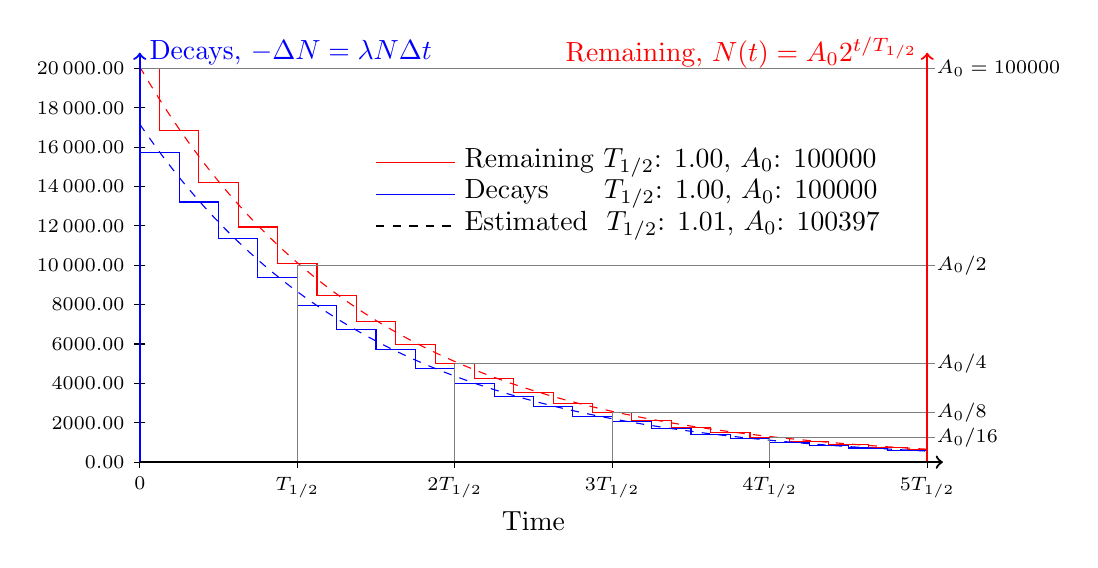
\begin{tikzpicture}
\begin{scope}[]
\clip (0,0) rectangle (10,5);
\begin{scope}[draw=blue]
\pgfpathmoveto{ \pgfqpoint {12.5cm} {0.0cm}}
\pgfpathlineto{ \pgfqpoint {12.5cm} {0.0645cm}}
\pgfpathlineto{ \pgfqpoint {12.0cm} {0.0645cm}}
\pgfpathlineto{ \pgfqpoint {12.0cm} {0.0705cm}}
\pgfpathlineto{ \pgfqpoint {11.5cm} {0.0705cm}}
\pgfpathlineto{ \pgfqpoint {11.5cm} {0.0785cm}}
\pgfpathlineto{ \pgfqpoint {11.0cm} {0.0785cm}}
\pgfpathlineto{ \pgfqpoint {11.0cm} {0.1065cm}}
\pgfpathlineto{ \pgfqpoint {10.5cm} {0.1065cm}}
\pgfpathlineto{ \pgfqpoint {10.5cm} {0.12675cm}}
\pgfpathlineto{ \pgfqpoint {10.0cm} {0.12675cm}}
\pgfpathlineto{ \pgfqpoint {10.0cm} {0.14275cm}}
\pgfpathlineto{ \pgfqpoint {9.5cm} {0.14275cm}}
\pgfpathlineto{ \pgfqpoint {9.5cm} {0.179cm}}
\pgfpathlineto{ \pgfqpoint {9.0cm} {0.179cm}}
\pgfpathlineto{ \pgfqpoint {9.0cm} {0.208cm}}
\pgfpathlineto{ \pgfqpoint {8.5cm} {0.208cm}}
\pgfpathlineto{ \pgfqpoint {8.5cm} {0.2525cm}}
\pgfpathlineto{ \pgfqpoint {8.0cm} {0.2525cm}}
\pgfpathlineto{ \pgfqpoint {8.0cm} {0.29925cm}}
\pgfpathlineto{ \pgfqpoint {7.5cm} {0.29925cm}}
\pgfpathlineto{ \pgfqpoint {7.5cm} {0.355cm}}
\pgfpathlineto{ \pgfqpoint {7.0cm} {0.355cm}}
\pgfpathlineto{ \pgfqpoint {7.0cm} {0.426cm}}
\pgfpathlineto{ \pgfqpoint {6.5cm} {0.426cm}}
\pgfpathlineto{ \pgfqpoint {6.5cm} {0.51525cm}}
\pgfpathlineto{ \pgfqpoint {6.0cm} {0.51525cm}}
\pgfpathlineto{ \pgfqpoint {6.0cm} {0.584cm}}
\pgfpathlineto{ \pgfqpoint {5.5cm} {0.584cm}}
\pgfpathlineto{ \pgfqpoint {5.5cm} {0.708cm}}
\pgfpathlineto{ \pgfqpoint {5.0cm} {0.708cm}}
\pgfpathlineto{ \pgfqpoint {5.0cm} {0.83375cm}}
\pgfpathlineto{ \pgfqpoint {4.5cm} {0.83375cm}}
\pgfpathlineto{ \pgfqpoint {4.5cm} {1.00275cm}}
\pgfpathlineto{ \pgfqpoint {4.0cm} {1.00275cm}}
\pgfpathlineto{ \pgfqpoint {4.0cm} {1.185cm}}
\pgfpathlineto{ \pgfqpoint {3.5cm} {1.185cm}}
\pgfpathlineto{ \pgfqpoint {3.5cm} {1.43475cm}}
\pgfpathlineto{ \pgfqpoint {3.0cm} {1.43475cm}}
\pgfpathlineto{ \pgfqpoint {3.0cm} {1.689cm}}
\pgfpathlineto{ \pgfqpoint {2.5cm} {1.689cm}}
\pgfpathlineto{ \pgfqpoint {2.5cm} {1.9935cm}}
\pgfpathlineto{ \pgfqpoint {2.0cm} {1.9935cm}}
\pgfpathlineto{ \pgfqpoint {2.0cm} {2.33975cm}}
\pgfpathlineto{ \pgfqpoint {1.5cm} {2.33975cm}}
\pgfpathlineto{ \pgfqpoint {1.5cm} {2.83525cm}}
\pgfpathlineto{ \pgfqpoint {1.0cm} {2.83525cm}}
\pgfpathlineto{ \pgfqpoint {1.0cm} {3.30425cm}}
\pgfpathlineto{ \pgfqpoint {0.5cm} {3.30425cm}}
\pgfpathlineto{ \pgfqpoint {0.5cm} {3.93175cm}}
\pgfpathlineto{ \pgfqpoint {0.0cm} {3.93175cm}}
\pgfpathlineto{ \pgfqpoint {0.0cm} {0.0cm}}
\pgfusepath{ stroke }
\end{scope}
\begin{scope}[draw=red]
\pgfpathmoveto{ \pgfqpoint {12.25cm} {0.0cm}}
\pgfpathlineto{ \pgfqpoint {12.25cm} {0.07965000152587891cm}}
\pgfpathlineto{ \pgfqpoint {11.75cm} {0.07965000152587891cm}}
\pgfpathlineto{ \pgfqpoint {11.75cm} {0.09375cm}}
\pgfpathlineto{ \pgfqpoint {11.25cm} {0.09375cm}}
\pgfpathlineto{ \pgfqpoint {11.25cm} {0.10945000457763672cm}}
\pgfpathlineto{ \pgfqpoint {10.75cm} {0.10945000457763672cm}}
\pgfpathlineto{ \pgfqpoint {10.75cm} {0.13075cm}}
\pgfpathlineto{ \pgfqpoint {10.25cm} {0.13075cm}}
\pgfpathlineto{ \pgfqpoint {10.25cm} {0.15610000610351563cm}}
\pgfpathlineto{ \pgfqpoint {9.75cm} {0.15610000610351563cm}}
\pgfpathlineto{ \pgfqpoint {9.75cm} {0.18465000915527344cm}}
\pgfpathlineto{ \pgfqpoint {9.25cm} {0.18465000915527344cm}}
\pgfpathlineto{ \pgfqpoint {9.25cm} {0.2204499969482422cm}}
\pgfpathlineto{ \pgfqpoint {8.75cm} {0.2204499969482422cm}}
\pgfpathlineto{ \pgfqpoint {8.75cm} {0.26205001831054686cm}}
\pgfpathlineto{ \pgfqpoint {8.25cm} {0.26205001831054686cm}}
\pgfpathlineto{ \pgfqpoint {8.25cm} {0.31255001831054685cm}}
\pgfpathlineto{ \pgfqpoint {7.75cm} {0.31255001831054685cm}}
\pgfpathlineto{ \pgfqpoint {7.75cm} {0.37239999389648437cm}}
\pgfpathlineto{ \pgfqpoint {7.25cm} {0.37239999389648437cm}}
\pgfpathlineto{ \pgfqpoint {7.25cm} {0.4433999938964844cm}}
\pgfpathlineto{ \pgfqpoint {6.75cm} {0.4433999938964844cm}}
\pgfpathlineto{ \pgfqpoint {6.75cm} {0.5286000366210938cm}}
\pgfpathlineto{ \pgfqpoint {6.25cm} {0.5286000366210938cm}}
\pgfpathlineto{ \pgfqpoint {6.25cm} {0.6316500244140625cm}}
\pgfpathlineto{ \pgfqpoint {5.75cm} {0.6316500244140625cm}}
\pgfpathlineto{ \pgfqpoint {5.75cm} {0.7484500122070312cm}}
\pgfpathlineto{ \pgfqpoint {5.25cm} {0.7484500122070312cm}}
\pgfpathlineto{ \pgfqpoint {5.25cm} {0.8900499877929687cm}}
\pgfpathlineto{ \pgfqpoint {4.75cm} {0.8900499877929687cm}}
\pgfpathlineto{ \pgfqpoint {4.75cm} {1.056800048828125cm}}
\pgfpathlineto{ \pgfqpoint {4.25cm} {1.056800048828125cm}}
\pgfpathlineto{ \pgfqpoint {4.25cm} {1.2573499755859374cm}}
\pgfpathlineto{ \pgfqpoint {3.75cm} {1.2573499755859374cm}}
\pgfpathlineto{ \pgfqpoint {3.75cm} {1.4943499755859375cm}}
\pgfpathlineto{ \pgfqpoint {3.25cm} {1.4943499755859375cm}}
\pgfpathlineto{ \pgfqpoint {3.25cm} {1.781300048828125cm}}
\pgfpathlineto{ \pgfqpoint {2.75cm} {1.781300048828125cm}}
\pgfpathlineto{ \pgfqpoint {2.75cm} {2.11910009765625cm}}
\pgfpathlineto{ \pgfqpoint {2.25cm} {2.11910009765625cm}}
\pgfpathlineto{ \pgfqpoint {2.25cm} {2.517800048828125cm}}
\pgfpathlineto{ \pgfqpoint {1.75cm} {2.517800048828125cm}}
\pgfpathlineto{ \pgfqpoint {1.75cm} {2.98575cm}}
\pgfpathlineto{ \pgfqpoint {1.25cm} {2.98575cm}}
\pgfpathlineto{ \pgfqpoint {1.25cm} {3.552800048828125cm}}
\pgfpathlineto{ \pgfqpoint {0.75cm} {3.552800048828125cm}}
\pgfpathlineto{ \pgfqpoint {0.75cm} {4.21364990234375cm}}
\pgfpathlineto{ \pgfqpoint {0.25cm} {4.21364990234375cm}}
\pgfpathlineto{ \pgfqpoint {0.25cm} {5.0cm}}
\pgfpathlineto{ \pgfqpoint {-0.25cm} {5.0cm}}
\pgfpathlineto{ \pgfqpoint {-0.25cm} {0.0cm}}
\pgfusepath{ stroke }
\end{scope}
\begin{scope}[blue,dashed]
\pgfpathmoveto{ \pgfqpoint {0.0cm} {4.291669184266502cm}}
\pgfpathlineto{ \pgfqpoint {0.1cm} {4.14738628976011cm}}
\pgfpathlineto{ \pgfqpoint {0.2cm} {4.007954084520137cm}}
\pgfpathlineto{ \pgfqpoint {0.3cm} {3.8732094917907434cm}}
\pgfpathlineto{ \pgfqpoint {0.4cm} {3.7429949173417323cm}}
\pgfpathlineto{ \pgfqpoint {0.5cm} {3.6171580651499013cm}}
\pgfpathlineto{ \pgfqpoint {0.6cm} {3.4955517592770584cm}}
\pgfpathlineto{ \pgfqpoint {0.7cm} {3.3780337717363658cm}}
\pgfpathlineto{ \pgfqpoint {0.8cm} {3.264466656145706cm}}
\pgfpathlineto{ \pgfqpoint {0.9cm} {3.1547175869734967cm}}
\pgfpathlineto{ \pgfqpoint {1.0cm} {3.0486582041889516cm}}
\pgfpathlineto{ \pgfqpoint {1.1cm} {2.946164463135092cm}}
\pgfpathlineto{ \pgfqpoint {1.2cm} {2.8471164894489163cm}}
\pgfpathlineto{ \pgfqpoint {1.3cm} {2.7513984388590553cm}}
\pgfpathlineto{ \pgfqpoint {1.4cm} {2.6588983616969335cm}}
\pgfpathlineto{ \pgfqpoint {1.5cm} {2.5695080719629626cm}}
\pgfpathlineto{ \pgfqpoint {1.6cm} {2.483123020794645cm}}
\pgfpathlineto{ \pgfqpoint {1.7cm} {2.399642174188585cm}}
\pgfpathlineto{ \pgfqpoint {1.8cm} {2.318967894833403cm}}
\pgfpathlineto{ \pgfqpoint {1.9cm} {2.241005827915344cm}}
\pgfpathlineto{ \pgfqpoint {2.0cm} {2.1656647907630173cm}}
\pgfpathlineto{ \pgfqpoint {2.1cm} {2.0928566662022066cm}}
\pgfpathlineto{ \pgfqpoint {2.2cm} {2.0224962994960154cm}}
\pgfpathlineto{ \pgfqpoint {2.3cm} {1.9545013987498094cm}}
\pgfpathlineto{ \pgfqpoint {2.4cm} {1.8887924386644783cm}}
\pgfpathlineto{ \pgfqpoint {2.5cm} {1.8252925675254414cm}}
\pgfpathlineto{ \pgfqpoint {2.6cm} {1.7639275173186217cm}}
\pgfpathlineto{ \pgfqpoint {2.7cm} {1.7046255168682534cm}}
\pgfpathlineto{ \pgfqpoint {2.8cm} {1.6473172078949372cm}}
\pgfpathlineto{ \pgfqpoint {2.9cm} {1.5919355638957637cm}}
\pgfpathlineto{ \pgfqpoint {3.0cm} {1.5384158117516333cm}}
\pgfpathlineto{ \pgfqpoint {3.1cm} {1.4866953559700764cm}}
\pgfpathlineto{ \pgfqpoint {3.2cm} {1.4367137054749826cm}}
\pgfpathlineto{ \pgfqpoint {3.3cm} {1.388412402857604cm}}
\pgfpathlineto{ \pgfqpoint {3.4cm} {1.3417349560060927cm}}
\pgfpathlineto{ \pgfqpoint {3.5cm} {1.296626772033601cm}}
\pgfpathlineto{ \pgfqpoint {3.6cm} {1.2530350934276786cm}}
\pgfpathlineto{ \pgfqpoint {3.7cm} {1.2109089363462744cm}}
\pgfpathlineto{ \pgfqpoint {3.8cm} {1.1701990309881898cm}}
\pgfpathlineto{ \pgfqpoint {3.9cm} {1.130857763968233cm}}
\pgfpathlineto{ \pgfqpoint {4.0cm} {1.0928391226296763cm}}
\pgfpathlineto{ \pgfqpoint {4.1cm} {1.0560986412288984cm}}
\pgfpathlineto{ \pgfqpoint {4.2cm} {1.0205933489292507cm}}
\pgfpathlineto{ \pgfqpoint {4.3cm} {0.9862817195433402cm}}
\pgfpathlineto{ \pgfqpoint {4.4cm} {0.9531236229649396cm}}
\pgfpathlineto{ \pgfqpoint {4.5cm} {0.9210802782337211cm}}
\pgfpathlineto{ \pgfqpoint {4.6cm} {0.8901142081779211cm}}
\pgfpathlineto{ \pgfqpoint {4.7cm} {0.8601891955818896cm}}
\pgfpathlineto{ \pgfqpoint {4.8cm} {0.8312702408272509cm}}
\pgfpathlineto{ \pgfqpoint {4.9cm} {0.8033235209581423cm}}
\pgfpathlineto{ \pgfqpoint {5.0cm} {0.7763163501226493cm}}
\pgfpathlineto{ \pgfqpoint {5.1cm} {0.7502171413441711cm}}
\pgfpathlineto{ \pgfqpoint {5.2cm} {0.724995369578007cm}}
\pgfpathlineto{ \pgfqpoint {5.3cm} {0.700621536009956cm}}
\pgfpathlineto{ \pgfqpoint {5.4cm} {0.6770671335551663cm}}
\pgfpathlineto{ \pgfqpoint {5.5cm} {0.6543046135168983cm}}
\pgfpathlineto{ \pgfqpoint {5.6cm} {0.6323073533661862cm}}
\pgfpathlineto{ \pgfqpoint {5.7cm} {0.6110496256047343cm}}
\pgfpathlineto{ \pgfqpoint {5.8cm} {0.5905065676746142cm}}
\pgfpathlineto{ \pgfqpoint {5.9cm} {0.5706541528795792cm}}
\pgfpathlineto{ \pgfqpoint {6.0cm} {0.5514691622839839cm}}
\pgfpathlineto{ \pgfqpoint {6.1cm} {0.532929157556442cm}}
\pgfpathlineto{ \pgfqpoint {6.2cm} {0.5150124547264592cm}}
\pgfpathlineto{ \pgfqpoint {6.3cm} {0.497698098823355cm}}
\pgfpathlineto{ \pgfqpoint {6.4cm} {0.48096583936779874cm}}
\pgfpathlineto{ \pgfqpoint {6.5cm} {0.46479610668730975cm}}
\pgfpathlineto{ \pgfqpoint {6.6cm} {0.4491699890280082cm}}
\pgfpathlineto{ \pgfqpoint {6.7cm} {0.43406921043585733cm}}
\pgfpathlineto{ \pgfqpoint {6.8cm} {0.4194761093815194cm}}
\pgfpathlineto{ \pgfqpoint {6.9cm} {0.4053736181038302cm}}
\pgfpathlineto{ \pgfqpoint {7.0cm} {0.39174524264773236cm}}
\pgfpathlineto{ \pgfqpoint {7.1cm} {0.37857504357331695cm}}
\pgfpathlineto{ \pgfqpoint {7.2cm} {0.365847617313416cm}}
\pgfpathlineto{ \pgfqpoint {7.3cm} {0.3535480781579374cm}}
\pgfpathlineto{ \pgfqpoint {7.4cm} {0.34166204084387597cm}}
\pgfpathlineto{ \pgfqpoint {7.5cm} {0.330175603730634cm}}
\pgfpathlineto{ \pgfqpoint {7.6cm} {0.3190753325409773cm}}
\pgfpathlineto{ \pgfqpoint {7.7cm} {0.3083482446486074cm}}
\pgfpathlineto{ \pgfqpoint {7.8cm} {0.29798179389397655cm}}
\pgfpathlineto{ \pgfqpoint {7.9cm} {0.28796385591058116cm}}
\pgfpathlineto{ \pgfqpoint {8.0cm} {0.27828271394457926cm}}
\pgfpathlineto{ \pgfqpoint {8.1cm} {0.2689270451511374cm}}
\pgfpathlineto{ \pgfqpoint {8.2cm} {0.2598859073514892cm}}
\pgfpathlineto{ \pgfqpoint {8.3cm} {0.25114872623520945cm}}
\pgfpathlineto{ \pgfqpoint {8.4cm} {0.24270528299274cm}}
\pgfpathlineto{ \pgfqpoint {8.5cm} {0.23454570236370076cm}}
\pgfpathlineto{ \pgfqpoint {8.6cm} {0.22666044108700867cm}}
\pgfpathlineto{ \pgfqpoint {8.7cm} {0.21904027673929508cm}}
\pgfpathlineto{ \pgfqpoint {8.8cm} {0.21167629694856746cm}}
\pgfpathlineto{ \pgfqpoint {8.9cm} {0.2045598889705015cm}}
\pgfpathlineto{ \pgfqpoint {9.0cm} {0.19768272961516925cm}}
\pgfpathlineto{ \pgfqpoint {9.1cm} {0.19103677551242404cm}}
\pgfpathlineto{ \pgfqpoint {9.2cm} {0.1846142537045575cm}}
\pgfpathlineto{ \pgfqpoint {9.3cm} {0.17840765255522312cm}}
\pgfpathlineto{ \pgfqpoint {9.4cm} {0.17240971296399685cm}}
\pgfpathlineto{ \pgfqpoint {9.5cm} {0.16661341987629624cm}}
\pgfpathlineto{ \pgfqpoint {9.6cm} {0.16101199407873223cm}}
\pgfpathlineto{ \pgfqpoint {9.7cm} {0.1555988842702939cm}}
\pgfpathlineto{ \pgfqpoint {9.8cm} {0.15036775940009495cm}}
\pgfpathlineto{ \pgfqpoint {9.9cm} {0.14531250126271952cm}}
\pgfpathlineto{ \pgfqpoint {10.0cm} {0.1404271973425078cm}}
\pgfusepath{ stroke }
\end{scope}
\begin{scope}[red,dashed]
\pgfpathmoveto{ \pgfqpoint {0.0cm} {5.019875113962694cm}}
\pgfpathlineto{ \pgfqpoint {0.1cm} {4.851110449118908cm}}
\pgfpathlineto{ \pgfqpoint {0.2cm} {4.688019533412946cm}}
\pgfpathlineto{ \pgfqpoint {0.3cm} {4.530411619395937cm}}
\pgfpathlineto{ \pgfqpoint {0.4cm} {4.3781023724138555cm}}
\pgfpathlineto{ \pgfqpoint {0.5cm} {4.230913655013882cm}}
\pgfpathlineto{ \pgfqpoint {0.6cm} {4.088673318598868cm}}
\pgfpathlineto{ \pgfqpoint {0.7cm} {3.9512150020862165cm}}
\pgfpathlineto{ \pgfqpoint {0.8cm} {3.8183779373357294cm}}
\pgfpathlineto{ \pgfqpoint {0.9cm} {3.690006761118823cm}}
\pgfpathlineto{ \pgfqpoint {1.0cm} {3.5659513334092017cm}}
\pgfpathlineto{ \pgfqpoint {1.1cm} {3.446066561782485cm}}
\pgfpathlineto{ \pgfqpoint {1.2cm} {3.3302122317193805cm}}
\pgfpathlineto{ \pgfqpoint {1.3cm} {3.2182528426139534cm}}
\pgfpathlineto{ \pgfqpoint {1.4cm} {3.1100574492951822cm}}
\pgfpathlineto{ \pgfqpoint {1.5cm} {3.0054995088764436cm}}
\pgfpathlineto{ \pgfqpoint {1.6cm} {2.904456732753813cm}}
\pgfpathlineto{ \pgfqpoint {1.7cm} {2.8068109435800794cm}}
\pgfpathlineto{ \pgfqpoint {1.8cm} {2.7124479370471866cm}}
\pgfpathlineto{ \pgfqpoint {1.9cm} {2.6212573483154635cm}}
\pgfpathlineto{ \pgfqpoint {2.0cm} {2.533132522933391cm}}
\pgfpathlineto{ \pgfqpoint {2.1cm} {2.4479703920969778cm}}
\pgfpathlineto{ \pgfqpoint {2.2cm} {2.3656713521028068cm}}
\pgfpathlineto{ \pgfqpoint {2.3cm} {2.286139147853802cm}}
\pgfpathlineto{ \pgfqpoint {2.4cm} {2.2092807602814393cm}}
\pgfpathlineto{ \pgfqpoint {2.5cm} {2.135006297552745cm}}
\pgfpathlineto{ \pgfqpoint {2.6cm} {2.0632288899348428cm}}
\pgfpathlineto{ \pgfqpoint {2.7cm} {1.9938645881940769cm}}
\pgfpathlineto{ \pgfqpoint {2.8cm} {1.9268322654108838cm}}
\pgfpathlineto{ \pgfqpoint {2.9cm} {1.8620535220955816cm}}
\pgfpathlineto{ \pgfqpoint {3.0cm} {1.7994525944941013cm}}
\pgfpathlineto{ \pgfqpoint {3.1cm} {1.7389562659764084cm}}
\pgfpathlineto{ \pgfqpoint {3.2cm} {1.6804937814039902cm}}
\pgfpathlineto{ \pgfqpoint {3.3cm} {1.6239967643762436cm}}
\pgfpathlineto{ \pgfqpoint {3.4cm} {1.5693991372589837cm}}
\pgfpathlineto{ \pgfqpoint {3.5cm} {1.5166370439015335cm}}
\pgfpathlineto{ \pgfqpoint {3.6cm} {1.4656487749520175cm}}
\pgfpathlineto{ \pgfqpoint {3.7cm} {1.4163746956834946cm}}
\pgfpathlineto{ \pgfqpoint {3.8cm} {1.3687571762465318cm}}
\pgfpathlineto{ \pgfqpoint {3.9cm} {1.3227405242666337cm}}
\pgfpathlineto{ \pgfqpoint {4.0cm} {1.2782709197077cm}}
\pgfpathlineto{ \pgfqpoint {4.1cm} {1.235296351925329cm}}
\pgfpathlineto{ \pgfqpoint {4.2cm} {1.193766558836341cm}}
\pgfpathlineto{ \pgfqpoint {4.3cm} {1.1536329681333846cm}}
\pgfpathlineto{ \pgfqpoint {4.4cm} {1.1148486404758622cm}}
\pgfpathlineto{ \pgfqpoint {4.5cm} {1.0773682145907377cm}}
\pgfpathlineto{ \pgfqpoint {4.6cm} {1.0411478542190187cm}}
\pgfpathlineto{ \pgfqpoint {4.7cm} {1.0061451968458563cm}}
\pgfpathlineto{ \pgfqpoint {4.8cm} {0.9723193041543079cm}}
\pgfpathlineto{ \pgfqpoint {4.9cm} {0.9396306141448049cm}}
\pgfpathlineto{ \pgfqpoint {5.0cm} {0.9080408948643329cm}}
\pgfpathlineto{ \pgfqpoint {5.1cm} {0.8775131996912039cm}}
\pgfpathlineto{ \pgfqpoint {5.2cm} {0.848011824123121cm}}
\pgfpathlineto{ \pgfqpoint {5.3cm} {0.8195022640180032cm}}
\pgfpathlineto{ \pgfqpoint {5.4cm} {0.7919511752387154cm}}
\pgfpathlineto{ \pgfqpoint {5.5cm} {0.7653263346545247cm}}
\pgfpathlineto{ \pgfqpoint {5.6cm} {0.7395966024536501cm}}
\pgfpathlineto{ \pgfqpoint {5.7cm} {0.7147318857228464cm}}
\pgfpathlineto{ \pgfqpoint {5.8cm} {0.6907031032514106cm}}
\pgfpathlineto{ \pgfqpoint {5.9cm} {0.667482151518456cm}}
\pgfpathlineto{ \pgfqpoint {6.0cm} {0.6450418718236695cm}}
\pgfpathlineto{ \pgfqpoint {6.1cm} {0.6233560185231092cm}}
\pgfpathlineto{ \pgfqpoint {6.2cm} {0.6023992283328915cm}}
\pgfpathlineto{ \pgfqpoint {6.3cm} {0.5821469906648709cm}}
\pgfpathlineto{ \pgfqpoint {6.4cm} {0.5625756189596052cm}}
\pgfpathlineto{ \pgfqpoint {6.5cm} {0.5436622229830956cm}}
\pgfpathlineto{ \pgfqpoint {6.6cm} {0.5253846820548829cm}}
\pgfpathlineto{ \pgfqpoint {6.7cm} {0.5077216191762013cm}}
\pgfpathlineto{ \pgfqpoint {6.8cm} {0.49065237602792405cm}}
\pgfpathlineto{ \pgfqpoint {6.9cm} {0.4741569888090587cm}}
\pgfpathlineto{ \pgfqpoint {7.0cm} {0.45821616488753875cm}}
\pgfpathlineto{ \pgfqpoint {7.1cm} {0.44281126023599543cm}}
\pgfpathlineto{ \pgfqpoint {7.2cm} {0.4279242576261258cm}}
\pgfpathlineto{ \pgfqpoint {7.3cm} {0.4135377455561492cm}}
\pgfpathlineto{ \pgfqpoint {7.4cm} {0.39963489788670875cm}}
\pgfpathlineto{ \pgfqpoint {7.5cm} {0.38619945416139856cm}}
\pgfpathlineto{ \pgfqpoint {7.6cm} {0.3732157005889017cm}}
\pgfpathlineto{ \pgfqpoint {7.7cm} {0.36066845166449474cm}}
\pgfpathlineto{ \pgfqpoint {7.8cm} {0.34854303240942575cm}}
\pgfpathlineto{ \pgfqpoint {7.9cm} {0.33682526120738876cm}}
\pgfpathlineto{ \pgfqpoint {8.0cm} {0.3255014332180282cm}}
\pgfpathlineto{ \pgfqpoint {8.1cm} {0.3145583043480655cm}}
\pgfpathlineto{ \pgfqpoint {8.2cm} {0.30398307576130795cm}}
\pgfpathlineto{ \pgfqpoint {8.3cm} {0.29376337890941895cm}}
\pgfpathlineto{ \pgfqpoint {8.4cm} {0.2838872610659433cm}}
\pgfpathlineto{ \pgfqpoint {8.5cm} {0.27434317134666864cm}}
\pgfpathlineto{ \pgfqpoint {8.6cm} {0.26511994719997206cm}}
\pgfpathlineto{ \pgfqpoint {8.7cm} {0.2562068013513525cm}}
\pgfpathlineto{ \pgfqpoint {8.8cm} {0.24759330918687764cm}}
\pgfpathlineto{ \pgfqpoint {8.9cm} {0.23926939656079196cm}}
\pgfpathlineto{ \pgfqpoint {9.0cm} {0.2312253280130228cm}}
\pgfpathlineto{ \pgfqpoint {9.1cm} {0.2234516953828063cm}}
\pgfpathlineto{ \pgfqpoint {9.2cm} {0.21593940680511567cm}}
\pgfpathlineto{ \pgfqpoint {9.3cm} {0.20867967607702115cm}}
\pgfpathlineto{ \pgfqpoint {9.4cm} {0.2016640123815459cm}}
\pgfpathlineto{ \pgfqpoint {9.5cm} {0.19488421035699746cm}}
\pgfpathlineto{ \pgfqpoint {9.6cm} {0.1883323405001632cm}}
\pgfpathlineto{ \pgfqpoint {9.7cm} {0.1820007398921422cm}}
\pgfpathlineto{ \pgfqpoint {9.8cm} {0.1758820032359683cm}}
\pgfpathlineto{ \pgfqpoint {9.9cm} {0.16996897419554255cm}}
\pgfpathlineto{ \pgfqpoint {10.0cm} {0.1642547370257439cm}}
\pgfusepath{ stroke }
\end{scope}
\draw[blue] (3.0,3.4) -- (4.0,3.4);
\node[right,] at (4.0,3.4) {Decays\ \ \ \ \ \ $T_{1/2}$:  1.00, $A_0$: 100000};
\draw[black,thick,dashed] (3.0,3.0) -- (4.0,3.0);
\node[right,] at (4.0,3.0) {Estimated \ $T_{1/2}$:  1.01, $A_0$: 100397};
\draw[red] (3.0,3.8) -- (4.0,3.8);
\node[right,] at (4.0,3.8) {Remaining $T_{1/2}$:  1.00, $A_0$: 100000};
\end{scope}
\draw (0.0,0.0cm + 2pt) -- (0.0, 0.0cm-2pt) node[below] {\scriptsize $0$};
\draw (2.0,0.0cm + 2pt) -- (2.0, 0.0cm-2pt) node[below] {\scriptsize $T_{1/2}$};
\draw (4.0,0.0cm + 2pt) -- (4.0, 0.0cm-2pt) node[below] {\scriptsize $2T_{1/2}$};
\draw (6.0,0.0cm + 2pt) -- (6.0, 0.0cm-2pt) node[below] {\scriptsize $3T_{1/2}$};
\draw (8.0,0.0cm + 2pt) -- (8.0, 0.0cm-2pt) node[below] {\scriptsize $4T_{1/2}$};
\draw (10.0,0.0cm + 2pt) -- (10.0, 0.0cm-2pt) node[below] {\scriptsize $5T_{1/2}$};
\draw (0.0cm + 2pt,0.0) -- (0.0cm-2pt,0.0) node[left] {\scriptsize{\num[round-mode=places,round-precision=2]{0}}};
\draw (0.0cm + 2pt,0.5) -- (0.0cm-2pt,0.5) node[left] {\scriptsize{\num[round-mode=places,round-precision=2]{2000}}};
\draw (0.0cm + 2pt,1.0) -- (0.0cm-2pt,1.0) node[left] {\scriptsize{\num[round-mode=places,round-precision=2]{4000}}};
\draw (0.0cm + 2pt,1.5) -- (0.0cm-2pt,1.5) node[left] {\scriptsize{\num[round-mode=places,round-precision=2]{6000}}};
\draw (0.0cm + 2pt,2.0) -- (0.0cm-2pt,2.0) node[left] {\scriptsize{\num[round-mode=places,round-precision=2]{8000}}};
\draw (0.0cm + 2pt,2.5) -- (0.0cm-2pt,2.5) node[left] {\scriptsize{\num[round-mode=places,round-precision=2]{10000}}};
\draw (0.0cm + 2pt,3.0) -- (0.0cm-2pt,3.0) node[left] {\scriptsize{\num[round-mode=places,round-precision=2]{12000}}};
\draw (0.0cm + 2pt,3.5) -- (0.0cm-2pt,3.5) node[left] {\scriptsize{\num[round-mode=places,round-precision=2]{14000}}};
\draw (0.0cm + 2pt,4.0) -- (0.0cm-2pt,4.0) node[left] {\scriptsize{\num[round-mode=places,round-precision=2]{16000}}};
\draw (0.0cm + 2pt,4.5) -- (0.0cm-2pt,4.5) node[left] {\scriptsize{\num[round-mode=places,round-precision=2]{18000}}};
\draw (0.0cm + 2pt,5.0) -- (0.0cm-2pt,5.0) node[left] {\scriptsize{\num[round-mode=places,round-precision=2]{20000}}};
\draw[thin,gray] (0.0,5.0) -- (10.1,5.0);
\node[right] at (10.0,5.0) {\scriptsize{$A_0 = 100000$}};
\draw[thin,gray] (2.0,2.5) -- (10.1,2.5);
\draw[thin,gray] (2.0,0.0) -- (2.0,2.5);
\node[right] at (10.0,2.5) {\scriptsize{$A_0/2$}};
\draw[thin,gray] (4.0,1.25) -- (10.1,1.25);
\draw[thin,gray] (4.0,0.0) -- (4.0,1.25);
\node[right] at (10.0,1.25) {\scriptsize{$A_0/4$}};
\draw[thin,gray] (6.0,0.625) -- (10.1,0.625);
\draw[thin,gray] (6.0,0.0) -- (6.0,0.625);
\node[right] at (10.0,0.625) {\scriptsize{$A_0/8$}};
\draw[thin,gray] (8.0,0.3125) -- (10.1,0.3125);
\draw[thin,gray] (8.0,0.0) -- (8.0,0.3125);
\node[right] at (10.0,0.3125) {\scriptsize{$A_0/16$}};
\node[right,blue] at (0.0,5.2) {Decays, $-\Delta N = \lambda N \Delta t$};
\node[left,red] at (10.0,5.2) {Remaining, $N(t) = A_0 2^{t/T_{1/2}}$};
\node[below] at (5.0,-0.5) {Time};
\draw[blue,thick,->] (0.0,0.0) -- (0.0,5.2);
\draw[red,thick,->] (10.0,0.0) -- (10.0,5.2);
\draw[thick,->] (0.0,0.0) -- (10.2,0.0);
\end{tikzpicture}
%%% Local Variables: 
%%% mode: latex 
%%% TeX-master: "master" 
%%% End:


  \caption{ Attempt to show all data in one plot.}
\end{figure}

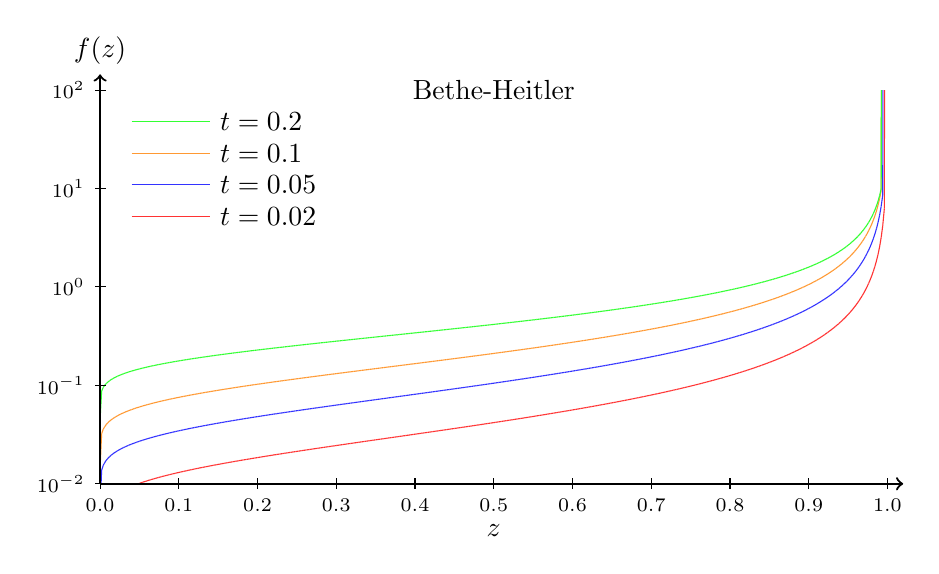
\begin{tikzpicture}
\begin{scope}[]
\clip (0,0) rectangle (10,5);
\begin{scope}[red!80]
\draw[] (0.000001,-0.88166773) -- (0.020000994,-0.37921697);
\draw[] (0.020000994,-0.37921697) -- (0.040000994,-0.3168717);
\draw[] (0.040000994,-0.3168717) -- (0.060000993,-0.2766621);
\draw[] (0.060000993,-0.2766621) -- (0.08000098,-0.24615079);
\draw[] (0.08000098,-0.24615079) -- (0.10000098,-0.22120506);
\draw[] (0.10000098,-0.22120506) -- (0.12000098,-0.19990832);
\draw[] (0.12000098,-0.19990832) -- (0.14000097,-0.18120557);
\draw[] (0.14000097,-0.18120557) -- (0.16000098,-0.1644504);
\draw[] (0.16000098,-0.1644504) -- (0.18000098,-0.14921606);
\draw[] (0.18000098,-0.14921606) -- (0.20000096,-0.13520539);
\draw[] (0.20000096,-0.13520539) -- (0.22000097,-0.12220144);
\draw[] (0.22000097,-0.12220144) -- (0.24000096,-0.110043585);
\draw[] (0.24000096,-0.110043585) -- (0.26000094,-0.09860605);
\draw[] (0.26000094,-0.09860605) -- (0.28000095,-0.087791085);
\draw[] (0.28000095,-0.087791085) -- (0.30000094,-0.07751852);
\draw[] (0.30000094,-0.07751852) -- (0.32000095,-0.06772518);
\draw[] (0.32000095,-0.06772518) -- (0.34000096,-0.05835682);
\draw[] (0.34000096,-0.05835682) -- (0.36000094,-0.04936874);
\draw[] (0.36000094,-0.04936874) -- (0.38000092,-0.04072368);
\draw[] (0.38000092,-0.04072368) -- (0.40000093,-0.032388866);
\draw[] (0.40000093,-0.032388866) -- (0.4200009,-0.024336576);
\draw[] (0.4200009,-0.024336576) -- (0.44000092,-0.016542673);
\draw[] (0.44000092,-0.016542673) -- (0.46000093,-0.008985996);
\draw[] (0.46000093,-0.008985996) -- (0.48000094,-0.0016480684);
\draw[] (0.48000094,-0.0016480684) -- (0.5000009,0.0054873526);
\draw[] (0.5000009,0.0054873526) -- (0.5200009,0.012435168);
\draw[] (0.5200009,0.012435168) -- (0.5400009,0.01920849);
\draw[] (0.5400009,0.01920849) -- (0.5600009,0.025818646);
\draw[] (0.5600009,0.025818646) -- (0.5800009,0.032276213);
\draw[] (0.5800009,0.032276213) -- (0.60000086,0.038591027);
\draw[] (0.60000086,0.038591027) -- (0.6200009,0.044771582);
\draw[] (0.6200009,0.044771582) -- (0.6400008,0.050825775);
\draw[] (0.6400008,0.050825775) -- (0.6600008,0.05676061);
\draw[] (0.6600008,0.05676061) -- (0.68000084,0.06258324);
\draw[] (0.68000084,0.06258324) -- (0.7000008,0.06829888);
\draw[] (0.7000008,0.06829888) -- (0.72000086,0.073913485);
\draw[] (0.72000086,0.073913485) -- (0.74000084,0.07943243);
\draw[] (0.74000084,0.07943243) -- (0.76000077,0.084860176);
\draw[] (0.76000077,0.084860176) -- (0.7800008,0.0902012);
\draw[] (0.7800008,0.0902012) -- (0.8000008,0.09545937);
\draw[] (0.8000008,0.09545937) -- (0.8200008,0.100639015);
\draw[] (0.8200008,0.100639015) -- (0.8400008,0.10574341);
\draw[] (0.8400008,0.10574341) -- (0.8600008,0.11077568);
\draw[] (0.8600008,0.11077568) -- (0.8800008,0.11573896);
\draw[] (0.8800008,0.11573896) -- (0.90000075,0.120636374);
\draw[] (0.90000075,0.120636374) -- (0.9200008,0.1254709);
\draw[] (0.9200008,0.1254709) -- (0.9400008,0.1302442);
\draw[] (0.9400008,0.1302442) -- (0.9600008,0.13495967);
\draw[] (0.9600008,0.13495967) -- (0.9800008,0.13961881);
\draw[] (0.9800008,0.13961881) -- (1.0000007,0.14422446);
\draw[] (1.0000007,0.14422446) -- (1.0200008,0.14877811);
\draw[] (1.0200008,0.14877811) -- (1.0400008,0.15328169);
\draw[] (1.0400008,0.15328169) -- (1.0600008,0.15773743);
\draw[] (1.0600008,0.15773743) -- (1.0800008,0.16214654);
\draw[] (1.0800008,0.16214654) -- (1.1000007,0.16651124);
\draw[] (1.1000007,0.16651124) -- (1.1200007,0.17083257);
\draw[] (1.1200007,0.17083257) -- (1.1400007,0.17511234);
\draw[] (1.1400007,0.17511234) -- (1.1600008,0.17935172);
\draw[] (1.1600008,0.17935172) -- (1.1800008,0.18355191);
\draw[] (1.1800008,0.18355191) -- (1.2000006,0.1877144);
\draw[] (1.2000006,0.1877144) -- (1.2200007,0.19184068);
\draw[] (1.2200007,0.19184068) -- (1.2400007,0.19593135);
\draw[] (1.2400007,0.19593135) -- (1.2600007,0.19998804);
\draw[] (1.2600007,0.19998804) -- (1.2800008,0.2040115);
\draw[] (1.2800008,0.2040115) -- (1.3000008,0.20800263);
\draw[] (1.3000008,0.20800263) -- (1.3200008,0.21196261);
\draw[] (1.3200008,0.21196261) -- (1.3400007,0.21589234);
\draw[] (1.3400007,0.21589234) -- (1.3600008,0.21979287);
\draw[] (1.3600008,0.21979287) -- (1.3800008,0.22366464);
\draw[] (1.3800008,0.22366464) -- (1.4000007,0.22750899);
\draw[] (1.4000007,0.22750899) -- (1.4200008,0.23132637);
\draw[] (1.4200008,0.23132637) -- (1.4400008,0.23511738);
\draw[] (1.4400008,0.23511738) -- (1.4600008,0.2388832);
\draw[] (1.4600008,0.2388832) -- (1.4800007,0.24262428);
\draw[] (1.4800007,0.24262428) -- (1.5000008,0.24634153);
\draw[] (1.5000008,0.24634153) -- (1.5200007,0.25003523);
\draw[] (1.5200007,0.25003523) -- (1.5400007,0.25370598);
\draw[] (1.5400007,0.25370598) -- (1.5600008,0.25735497);
\draw[] (1.5600008,0.25735497) -- (1.5800008,0.26098236);
\draw[] (1.5800008,0.26098236) -- (1.6000007,0.26458845);
\draw[] (1.6000007,0.26458845) -- (1.6200007,0.26817456);
\draw[] (1.6200007,0.26817456) -- (1.6400008,0.27174056);
\draw[] (1.6400008,0.27174056) -- (1.6600007,0.27528718);
\draw[] (1.6600007,0.27528718) -- (1.6800007,0.27881518);
\draw[] (1.6800007,0.27881518) -- (1.7000008,0.28232425);
\draw[] (1.7000008,0.28232425) -- (1.7200006,0.28581575);
\draw[] (1.7200006,0.28581575) -- (1.7400007,0.28928965);
\draw[] (1.7400007,0.28928965) -- (1.7600007,0.29274672);
\draw[] (1.7600007,0.29274672) -- (1.7800008,0.29618666);
\draw[] (1.7800008,0.29618666) -- (1.8000007,0.29961094);
\draw[] (1.8000007,0.29961094) -- (1.8200006,0.30301914);
\draw[] (1.8200006,0.30301914) -- (1.8400007,0.30641168);
\draw[] (1.8400007,0.30641168) -- (1.8600006,0.30978948);
\draw[] (1.8600006,0.30978948) -- (1.8800007,0.31315267);
\draw[] (1.8800007,0.31315267) -- (1.9000007,0.31650126);
\draw[] (1.9000007,0.31650126) -- (1.9200008,0.31983584);
\draw[] (1.9200008,0.31983584) -- (1.9400007,0.32315686);
\draw[] (1.9400007,0.32315686) -- (1.9600006,0.32646447);
\draw[] (1.9600006,0.32646447) -- (1.9800007,0.32975912);
\draw[] (1.9800007,0.32975912) -- (2.0000005,0.33304125);
\draw[] (2.0000005,0.33304125) -- (2.0200007,0.33631057);
\draw[] (2.0200007,0.33631057) -- (2.0400007,0.3395681);
\draw[] (2.0400007,0.3395681) -- (2.0600007,0.34281388);
\draw[] (2.0600007,0.34281388) -- (2.0800006,0.34604773);
\draw[] (2.0800006,0.34604773) -- (2.1000006,0.3492707);
\draw[] (2.1000006,0.3492707) -- (2.1200006,0.35248235);
\draw[] (2.1200006,0.35248235) -- (2.1400006,0.35568342);
\draw[] (2.1400006,0.35568342) -- (2.1600006,0.35887405);
\draw[] (2.1600006,0.35887405) -- (2.1800005,0.3620544);
\draw[] (2.1800005,0.3620544) -- (2.2000005,0.36522448);
\draw[] (2.2000005,0.36522448) -- (2.2200005,0.36838517);
\draw[] (2.2200005,0.36838517) -- (2.2400007,0.37153617);
\draw[] (2.2400007,0.37153617) -- (2.2600005,0.37467778);
\draw[] (2.2600005,0.37467778) -- (2.2800004,0.3778103);
\draw[] (2.2800004,0.3778103) -- (2.3000007,0.38093403);
\draw[] (2.3000007,0.38093403) -- (2.3200006,0.38404897);
\draw[] (2.3200006,0.38404897) -- (2.3400006,0.38715556);
\draw[] (2.3400006,0.38715556) -- (2.3600006,0.3902538);
\draw[] (2.3600006,0.3902538) -- (2.3800006,0.39334416);
\draw[] (2.3800006,0.39334416) -- (2.4000006,0.39642632);
\draw[] (2.4000006,0.39642632) -- (2.4200006,0.39950117);
\draw[] (2.4200006,0.39950117) -- (2.4400005,0.40256828);
\draw[] (2.4400005,0.40256828) -- (2.4600005,0.40562823);
\draw[] (2.4600005,0.40562823) -- (2.4800005,0.4086809);
\draw[] (2.4800005,0.4086809) -- (2.5000005,0.41172683);
\draw[] (2.5000005,0.41172683) -- (2.5200002,0.41476563);
\draw[] (2.5200002,0.41476563) -- (2.5400004,0.41779816);
\draw[] (2.5400004,0.41779816) -- (2.5600004,0.420824);
\draw[] (2.5600004,0.420824) -- (2.5800004,0.4238437);
\draw[] (2.5800004,0.4238437) -- (2.6000004,0.42685732);
\draw[] (2.6000004,0.42685732) -- (2.6200006,0.42986497);
\draw[] (2.6200006,0.42986497) -- (2.6400003,0.4328665);
\draw[] (2.6400003,0.4328665) -- (2.6600003,0.4358627);
\draw[] (2.6600003,0.4358627) -- (2.6800003,0.43885335);
\draw[] (2.6800003,0.43885335) -- (2.7000003,0.4418385);
\draw[] (2.7000003,0.4418385) -- (2.7200005,0.4448186);
\draw[] (2.7200005,0.4448186) -- (2.7400005,0.4477936);
\draw[] (2.7400005,0.4477936) -- (2.7600005,0.45076355);
\draw[] (2.7600005,0.45076355) -- (2.7800002,0.45372874);
\draw[] (2.7800002,0.45372874) -- (2.8000002,0.4566893);
\draw[] (2.8000002,0.4566893) -- (2.8200004,0.45964524);
\draw[] (2.8200004,0.45964524) -- (2.8400004,0.46259686);
\draw[] (2.8400004,0.46259686) -- (2.8600004,0.4655443);
\draw[] (2.8600004,0.4655443) -- (2.8800004,0.46848744);
\draw[] (2.8800004,0.46848744) -- (2.9,0.47142655);
\draw[] (2.9,0.47142655) -- (2.9200003,0.47436178);
\draw[] (2.9200003,0.47436178) -- (2.9400003,0.47729343);
\draw[] (2.9400003,0.47729343) -- (2.9600003,0.4802212);
\draw[] (2.9600003,0.4802212) -- (2.9800003,0.48314556);
\draw[] (2.9800003,0.48314556) -- (3.0000005,0.4860665);
\draw[] (3.0000005,0.4860665) -- (3.0200005,0.48898414);
\draw[] (3.0200005,0.48898414) -- (3.0400002,0.4918985);
\draw[] (3.0400002,0.4918985) -- (3.0600002,0.4948099);
\draw[] (3.0600002,0.4948099) -- (3.0800002,0.4977183);
\draw[] (3.0800002,0.4977183) -- (3.1000004,0.5006239);
\draw[] (3.1000004,0.5006239) -- (3.1200004,0.5035266);
\draw[] (3.1200004,0.5035266) -- (3.1400003,0.5064268);
\draw[] (3.1400003,0.5064268) -- (3.1600003,0.5093245);
\draw[] (3.1600003,0.5093245) -- (3.18,0.5122198);
\draw[] (3.18,0.5122198) -- (3.2000003,0.5151126);
\draw[] (3.2000003,0.5151126) -- (3.2200003,0.5180034);
\draw[] (3.2200003,0.5180034) -- (3.2400002,0.52089214);
\draw[] (3.2400002,0.52089214) -- (3.2600002,0.5237786);
\draw[] (3.2600002,0.5237786) -- (3.2800004,0.52666336);
\draw[] (3.2800004,0.52666336) -- (3.3000004,0.52954626);
\draw[] (3.3000004,0.52954626) -- (3.3200002,0.53242743);
\draw[] (3.3200002,0.53242743) -- (3.3400002,0.53530693);
\draw[] (3.3400002,0.53530693) -- (3.3600001,0.53818494);
\draw[] (3.3600001,0.53818494) -- (3.3800004,0.5410616);
\draw[] (3.3800004,0.5410616) -- (3.4000003,0.5439368);
\draw[] (3.4000003,0.5439368) -- (3.4200003,0.5468109);
\draw[] (3.4200003,0.5468109) -- (3.44,0.5496837);
\draw[] (3.44,0.5496837) -- (3.46,0.5525556);
\draw[] (3.46,0.5525556) -- (3.4800003,0.5554265);
\draw[] (3.4800003,0.5554265) -- (3.5000002,0.55829656);
\draw[] (3.5000002,0.55829656) -- (3.5200002,0.5611658);
\draw[] (3.5200002,0.5611658) -- (3.5400002,0.5640344);
\draw[] (3.5400002,0.5640344) -- (3.5600004,0.56690246);
\draw[] (3.5600004,0.56690246) -- (3.5800002,0.56976986);
\draw[] (3.5800002,0.56976986) -- (3.6000001,0.57263684);
\draw[] (3.6000001,0.57263684) -- (3.6200001,0.5755035);
\draw[] (3.6200001,0.5755035) -- (3.64,0.5783699);
\draw[] (3.64,0.5783699) -- (3.6600003,0.5812363);
\draw[] (3.6600003,0.5812363) -- (3.6800003,0.5841026);
\draw[] (3.6800003,0.5841026) -- (3.7000003,0.58696866);
\draw[] (3.7000003,0.58696866) -- (3.72,0.58983487);
\draw[] (3.72,0.58983487) -- (3.74,0.59270126);
\draw[] (3.74,0.59270126) -- (3.7600002,0.59556794);
\draw[] (3.7600002,0.59556794) -- (3.7800002,0.5984351);
\draw[] (3.7800002,0.5984351) -- (3.8000002,0.6013025);
\draw[] (3.8000002,0.6013025) -- (3.8200002,0.60417056);
\draw[] (3.8200002,0.60417056) -- (3.8400004,0.60703933);
\draw[] (3.8400004,0.60703933) -- (3.8600001,0.6099084);
\draw[] (3.8600001,0.6099084) -- (3.88,0.6127785);
\draw[] (3.88,0.6127785) -- (3.9,0.6156492);
\draw[] (3.9,0.6156492) -- (3.92,0.618521);
\draw[] (3.92,0.618521) -- (3.9400003,0.62139374);
\draw[] (3.9400003,0.62139374) -- (3.9600003,0.6242676);
\draw[] (3.9600003,0.6242676) -- (3.98,0.6271425);
\draw[] (3.98,0.6271425) -- (4.0,0.6300187);
\draw[] (4.0,0.6300187) -- (4.02,0.6328961);
\draw[] (4.02,0.6328961) -- (4.04,0.635775);
\draw[] (4.04,0.635775) -- (4.06,0.6386554);
\draw[] (4.06,0.6386554) -- (4.08,0.6415373);
\draw[] (4.08,0.6415373) -- (4.1000004,0.644421);
\draw[] (4.1000004,0.644421) -- (4.12,0.64730614);
\draw[] (4.12,0.64730614) -- (4.14,0.6501932);
\draw[] (4.14,0.6501932) -- (4.16,0.65308213);
\draw[] (4.16,0.65308213) -- (4.18,0.6559731);
\draw[] (4.18,0.6559731) -- (4.2000003,0.658866);
\draw[] (4.2000003,0.658866) -- (4.2200003,0.66176087);
\draw[] (4.2200003,0.66176087) -- (4.2400002,0.66465825);
\draw[] (4.2400002,0.66465825) -- (4.2599998,0.6675577);
\draw[] (4.2599998,0.6675577) -- (4.2799997,0.6704594);
\draw[] (4.2799997,0.6704594) -- (4.3,0.6733636);
\draw[] (4.3,0.6733636) -- (4.32,0.6762704);
\draw[] (4.32,0.6762704) -- (4.34,0.67917955);
\draw[] (4.34,0.67917955) -- (4.36,0.68209153);
\draw[] (4.36,0.68209153) -- (4.3799996,0.6850062);
\draw[] (4.3799996,0.6850062) -- (4.4,0.6879237);
\draw[] (4.4,0.6879237) -- (4.42,0.69084406);
\draw[] (4.42,0.69084406) -- (4.44,0.6937675);
\draw[] (4.44,0.6937675) -- (4.46,0.69669396);
\draw[] (4.46,0.69669396) -- (4.48,0.69962335);
\draw[] (4.48,0.69962335) -- (4.5,0.7025562);
\draw[] (4.5,0.7025562) -- (4.52,0.7054922);
\draw[] (4.52,0.7054922) -- (4.54,0.7084316);
\draw[] (4.54,0.7084316) -- (4.56,0.7113744);
\draw[] (4.56,0.7113744) -- (4.58,0.71432084);
\draw[] (4.58,0.71432084) -- (4.6,0.717271);
\draw[] (4.6,0.717271) -- (4.62,0.7202247);
\draw[] (4.62,0.7202247) -- (4.64,0.72318226);
\draw[] (4.64,0.72318226) -- (4.66,0.7261434);
\draw[] (4.66,0.7261434) -- (4.68,0.72910875);
\draw[] (4.68,0.72910875) -- (4.7,0.73207796);
\draw[] (4.7,0.73207796) -- (4.72,0.73505133);
\draw[] (4.72,0.73505133) -- (4.74,0.738029);
\draw[] (4.74,0.738029) -- (4.76,0.7410107);
\draw[] (4.76,0.7410107) -- (4.78,0.7439969);
\draw[] (4.78,0.7439969) -- (4.7999997,0.7469876);
\draw[] (4.7999997,0.7469876) -- (4.8199997,0.7499827);
\draw[] (4.8199997,0.7499827) -- (4.8399997,0.7529825);
\draw[] (4.8399997,0.7529825) -- (4.86,0.755987);
\draw[] (4.86,0.755987) -- (4.88,0.7589963);
\draw[] (4.88,0.7589963) -- (4.9,0.76201034);
\draw[] (4.9,0.76201034) -- (4.9199996,0.7650293);
\draw[] (4.9199996,0.7650293) -- (4.9399996,0.76805353);
\draw[] (4.9399996,0.76805353) -- (4.96,0.77108264);
\draw[] (4.96,0.77108264) -- (4.98,0.77411693);
\draw[] (4.98,0.77411693) -- (5.0,0.7771568);
\draw[] (5.0,0.7771568) -- (5.0200005,0.78020185);
\draw[] (5.0200005,0.78020185) -- (5.04,0.7832524);
\draw[] (5.04,0.7832524) -- (5.0600004,0.78630865);
\draw[] (5.0600004,0.78630865) -- (5.08,0.78937036);
\draw[] (5.08,0.78937036) -- (5.1000004,0.7924381);
\draw[] (5.1000004,0.7924381) -- (5.1200004,0.7955114);
\draw[] (5.1200004,0.7955114) -- (5.14,0.7985906);
\draw[] (5.14,0.7985906) -- (5.1600003,0.80167603);
\draw[] (5.1600003,0.80167603) -- (5.18,0.80476743);
\draw[] (5.18,0.80476743) -- (5.2000003,0.80786526);
\draw[] (5.2000003,0.80786526) -- (5.2200003,0.810969);
\draw[] (5.2200003,0.810969) -- (5.2400002,0.81407946);
\draw[] (5.2400002,0.81407946) -- (5.26,0.8171965);
\draw[] (5.26,0.8171965) -- (5.2799997,0.82031995);
\draw[] (5.2799997,0.82031995) -- (5.3,0.8234501);
\draw[] (5.3,0.8234501) -- (5.32,0.8265871);
\draw[] (5.32,0.8265871) -- (5.34,0.82973105);
\draw[] (5.34,0.82973105) -- (5.36,0.8328819);
\draw[] (5.36,0.8328819) -- (5.3800006,0.8360401);
\draw[] (5.3800006,0.8360401) -- (5.4,0.8392052);
\draw[] (5.4,0.8392052) -- (5.42,0.84237766);
\draw[] (5.42,0.84237766) -- (5.44,0.84555775);
\draw[] (5.44,0.84555775) -- (5.46,0.8487451);
\draw[] (5.46,0.8487451) -- (5.4800005,0.8519402);
\draw[] (5.4800005,0.8519402) -- (5.5,0.8551431);
\draw[] (5.5,0.8551431) -- (5.5200005,0.8583537);
\draw[] (5.5200005,0.8583537) -- (5.54,0.8615723);
\draw[] (5.54,0.8615723) -- (5.56,0.864799);
\draw[] (5.56,0.864799) -- (5.5800004,0.86803406);
\draw[] (5.5800004,0.86803406) -- (5.6,0.87127715);
\draw[] (5.6,0.87127715) -- (5.6200004,0.8745287);
\draw[] (5.6200004,0.8745287) -- (5.64,0.8777888);
\draw[] (5.64,0.8777888) -- (5.66,0.8810575);
\draw[] (5.66,0.8810575) -- (5.6800003,0.88433486);
\draw[] (5.6800003,0.88433486) -- (5.7,0.88762134);
\draw[] (5.7,0.88762134) -- (5.7200003,0.8909167);
\draw[] (5.7200003,0.8909167) -- (5.74,0.89422107);
\draw[] (5.74,0.89422107) -- (5.76,0.8975348);
\draw[] (5.76,0.8975348) -- (5.78,0.90085787);
\draw[] (5.78,0.90085787) -- (5.7999997,0.90419054);
\draw[] (5.7999997,0.90419054) -- (5.82,0.9075327);
\draw[] (5.82,0.9075327) -- (5.8399997,0.91088456);
\draw[] (5.8399997,0.91088456) -- (5.86,0.91424644);
\draw[] (5.86,0.91424644) -- (5.88,0.9176183);
\draw[] (5.88,0.9176183) -- (5.9,0.92100024);
\draw[] (5.9,0.92100024) -- (5.92,0.92439234);
\draw[] (5.92,0.92439234) -- (5.9399996,0.927795);
\draw[] (5.9399996,0.927795) -- (5.96,0.93120825);
\draw[] (5.96,0.93120825) -- (5.98,0.9346321);
\draw[] (5.98,0.9346321) -- (6.0,0.93806696);
\draw[] (6.0,0.93806696) -- (6.02,0.9415126);
\draw[] (6.02,0.9415126) -- (6.0400004,0.94496965);
\draw[] (6.0400004,0.94496965) -- (6.06,0.9484376);
\draw[] (6.06,0.9484376) -- (6.08,0.9519172);
\draw[] (6.08,0.9519172) -- (6.1,0.95540833);
\draw[] (6.1,0.95540833) -- (6.12,0.9589112);
\draw[] (6.12,0.9589112) -- (6.1400003,0.9624259);
\draw[] (6.1400003,0.9624259) -- (6.16,0.9659526);
\draw[] (6.16,0.9659526) -- (6.1800003,0.9694917);
\draw[] (6.1800003,0.9694917) -- (6.2,0.97304296);
\draw[] (6.2,0.97304296) -- (6.22,0.9766069);
\draw[] (6.22,0.9766069) -- (6.2400002,0.9801836);
\draw[] (6.2400002,0.9801836) -- (6.2599998,0.983773);
\draw[] (6.2599998,0.983773) -- (6.28,0.9873755);
\draw[] (6.28,0.9873755) -- (6.2999997,0.9909911);
\draw[] (6.2999997,0.9909911) -- (6.32,0.9946203);
\draw[] (6.32,0.9946203) -- (6.34,0.9982629);
\draw[] (6.34,0.9982629) -- (6.3599997,1.0019194);
\draw[] (6.3599997,1.0019194) -- (6.38,1.0055896);
\draw[] (6.38,1.0055896) -- (6.3999996,1.0092741);
\draw[] (6.3999996,1.0092741) -- (6.42,1.0129731);
\draw[] (6.42,1.0129731) -- (6.44,1.0166862);
\draw[] (6.44,1.0166862) -- (6.46,1.0204144);
\draw[] (6.46,1.0204144) -- (6.48,1.024157);
\draw[] (6.48,1.024157) -- (6.4999995,1.0279151);
\draw[] (6.4999995,1.0279151) -- (6.52,1.0316885);
\draw[] (6.52,1.0316885) -- (6.54,1.0354772);
\draw[] (6.54,1.0354772) -- (6.56,1.039282);
\draw[] (6.56,1.039282) -- (6.58,1.0431024);
\draw[] (6.58,1.0431024) -- (6.6000004,1.046939);
\draw[] (6.6000004,1.046939) -- (6.62,1.0507922);
\draw[] (6.62,1.0507922) -- (6.64,1.0546618);
\draw[] (6.64,1.0546618) -- (6.66,1.0585483);
\draw[] (6.66,1.0585483) -- (6.68,1.0624521);
\draw[] (6.68,1.0624521) -- (6.7000003,1.066373);
\draw[] (6.7000003,1.066373) -- (6.72,1.0703113);
\draw[] (6.72,1.0703113) -- (6.74,1.0742676);
\draw[] (6.74,1.0742676) -- (6.7599998,1.0782421);
\draw[] (6.7599998,1.0782421) -- (6.7799997,1.0822345);
\draw[] (6.7799997,1.0822345) -- (6.8,1.086246);
\draw[] (6.8,1.086246) -- (6.8199997,1.0902759);
\draw[] (6.8199997,1.0902759) -- (6.84,1.0943253);
\draw[] (6.84,1.0943253) -- (6.8599997,1.0983938);
\draw[] (6.8599997,1.0983938) -- (6.8799996,1.102482);
\draw[] (6.8799996,1.102482) -- (6.9,1.1065902);
\draw[] (6.9,1.1065902) -- (6.9199996,1.1107185);
\draw[] (6.9199996,1.1107185) -- (6.94,1.1148674);
\draw[] (6.94,1.1148674) -- (6.9599996,1.1190372);
\draw[] (6.9599996,1.1190372) -- (6.98,1.1232281);
\draw[] (6.98,1.1232281) -- (7.0,1.1274405);
\draw[] (7.0,1.1274405) -- (7.0199995,1.1316745);
\draw[] (7.0199995,1.1316745) -- (7.04,1.1359307);
\draw[] (7.04,1.1359307) -- (7.0599995,1.1402093);
\draw[] (7.0599995,1.1402093) -- (7.08,1.1445107);
\draw[] (7.08,1.1445107) -- (7.1,1.1488351);
\draw[] (7.1,1.1488351) -- (7.12,1.1531831);
\draw[] (7.12,1.1531831) -- (7.14,1.1575549);
\draw[] (7.14,1.1575549) -- (7.1599994,1.1619507);
\draw[] (7.1599994,1.1619507) -- (7.18,1.1663712);
\draw[] (7.18,1.1663712) -- (7.2,1.1708165);
\draw[] (7.2,1.1708165) -- (7.22,1.1752872);
\draw[] (7.22,1.1752872) -- (7.24,1.1797835);
\draw[] (7.24,1.1797835) -- (7.26,1.1843061);
\draw[] (7.26,1.1843061) -- (7.2799997,1.1888552);
\draw[] (7.2799997,1.1888552) -- (7.2999997,1.1934311);
\draw[] (7.2999997,1.1934311) -- (7.3199997,1.1980344);
\draw[] (7.3199997,1.1980344) -- (7.3399997,1.2026656);
\draw[] (7.3399997,1.2026656) -- (7.36,1.2073251);
\draw[] (7.36,1.2073251) -- (7.3799996,1.2120132);
\draw[] (7.3799996,1.2120132) -- (7.4,1.2167307);
\draw[] (7.4,1.2167307) -- (7.4199996,1.2214776);
\draw[] (7.4199996,1.2214776) -- (7.4399996,1.2262549);
\draw[] (7.4399996,1.2262549) -- (7.46,1.231063);
\draw[] (7.46,1.231063) -- (7.4799995,1.2359022);
\draw[] (7.4799995,1.2359022) -- (7.5,1.2407728);
\draw[] (7.5,1.2407728) -- (7.5199995,1.2456762);
\draw[] (7.5199995,1.2456762) -- (7.54,1.2506121);
\draw[] (7.54,1.2506121) -- (7.56,1.2555814);
\draw[] (7.56,1.2555814) -- (7.5799994,1.2605846);
\draw[] (7.5799994,1.2605846) -- (7.6,1.2656226);
\draw[] (7.6,1.2656226) -- (7.6199994,1.2706956);
\draw[] (7.6199994,1.2706956) -- (7.64,1.2758046);
\draw[] (7.64,1.2758046) -- (7.66,1.28095);
\draw[] (7.66,1.28095) -- (7.68,1.2861323);
\draw[] (7.68,1.2861323) -- (7.7,1.2913525);
\draw[] (7.7,1.2913525) -- (7.7199993,1.2966108);
\draw[] (7.7199993,1.2966108) -- (7.74,1.3019087);
\draw[] (7.74,1.3019087) -- (7.7599998,1.3072463);
\draw[] (7.7599998,1.3072463) -- (7.7799997,1.3126248);
\draw[] (7.7799997,1.3126248) -- (7.7999997,1.3180445);
\draw[] (7.7999997,1.3180445) -- (7.819999,1.3235065);
\draw[] (7.819999,1.3235065) -- (7.8399997,1.3290114);
\draw[] (7.8399997,1.3290114) -- (7.8599997,1.3345602);
\draw[] (7.8599997,1.3345602) -- (7.8799996,1.3401538);
\draw[] (7.8799996,1.3401538) -- (7.8999996,1.3457927);
\draw[] (7.8999996,1.3457927) -- (7.92,1.3514783);
\draw[] (7.92,1.3514783) -- (7.9399996,1.3572111);
\draw[] (7.9399996,1.3572111) -- (7.9599996,1.3629925);
\draw[] (7.9599996,1.3629925) -- (7.9799995,1.3688232);
\draw[] (7.9799995,1.3688232) -- (7.9999995,1.3747042);
\draw[] (7.9999995,1.3747042) -- (8.0199995,1.3806367);
\draw[] (8.0199995,1.3806367) -- (8.039999,1.3866216);
\draw[] (8.039999,1.3866216) -- (8.059999,1.3926601);
\draw[] (8.059999,1.3926601) -- (8.08,1.3987535);
\draw[] (8.08,1.3987535) -- (8.099999,1.4049023);
\draw[] (8.099999,1.4049023) -- (8.12,1.411109);
\draw[] (8.12,1.411109) -- (8.139999,1.4173735);
\draw[] (8.139999,1.4173735) -- (8.16,1.4236981);
\draw[] (8.16,1.4236981) -- (8.179999,1.4300834);
\draw[] (8.179999,1.4300834) -- (8.2,1.4365314);
\draw[] (8.2,1.4365314) -- (8.219999,1.4430429);
\draw[] (8.219999,1.4430429) -- (8.239999,1.4496198);
\draw[] (8.239999,1.4496198) -- (8.259999,1.4562637);
\draw[] (8.259999,1.4562637) -- (8.28,1.4629759);
\draw[] (8.28,1.4629759) -- (8.299999,1.4697583);
\draw[] (8.299999,1.4697583) -- (8.32,1.4766122);
\draw[] (8.32,1.4766122) -- (8.34,1.4835399);
\draw[] (8.34,1.4835399) -- (8.36,1.4905425);
\draw[] (8.36,1.4905425) -- (8.379999,1.4976226);
\draw[] (8.379999,1.4976226) -- (8.4,1.5047818);
\draw[] (8.4,1.5047818) -- (8.419999,1.5120221);
\draw[] (8.419999,1.5120221) -- (8.44,1.5193459);
\draw[] (8.44,1.5193459) -- (8.459999,1.5267551);
\draw[] (8.459999,1.5267551) -- (8.48,1.534252);
\draw[] (8.48,1.534252) -- (8.499999,1.5418389);
\draw[] (8.499999,1.5418389) -- (8.5199995,1.5495183);
\draw[] (8.5199995,1.5495183) -- (8.54,1.5572932);
\draw[] (8.54,1.5572932) -- (8.559999,1.5651655);
\draw[] (8.559999,1.5651655) -- (8.58,1.5731385);
\draw[] (8.58,1.5731385) -- (8.599999,1.5812148);
\draw[] (8.599999,1.5812148) -- (8.62,1.5893978);
\draw[] (8.62,1.5893978) -- (8.639999,1.5976901);
\draw[] (8.639999,1.5976901) -- (8.659999,1.6060954);
\draw[] (8.659999,1.6060954) -- (8.679999,1.6146171);
\draw[] (8.679999,1.6146171) -- (8.699999,1.6232587);
\draw[] (8.699999,1.6232587) -- (8.719999,1.632024);
\draw[] (8.719999,1.632024) -- (8.74,1.6409167);
\draw[] (8.74,1.6409167) -- (8.759999,1.6499412);
\draw[] (8.759999,1.6499412) -- (8.78,1.659102);
\draw[] (8.78,1.659102) -- (8.799999,1.6684031);
\draw[] (8.799999,1.6684031) -- (8.82,1.6778495);
\draw[] (8.82,1.6778495) -- (8.839999,1.6874465);
\draw[] (8.839999,1.6874465) -- (8.86,1.6971993);
\draw[] (8.86,1.6971993) -- (8.879999,1.7071129);
\draw[] (8.879999,1.7071129) -- (8.899999,1.7171937);
\draw[] (8.899999,1.7171937) -- (8.919999,1.7274477);
\draw[] (8.919999,1.7274477) -- (8.94,1.7378815);
\draw[] (8.94,1.7378815) -- (8.959999,1.7485023);
\draw[] (8.959999,1.7485023) -- (8.98,1.7593164);
\draw[] (8.98,1.7593164) -- (9.0,1.7703327);
\draw[] (9.0,1.7703327) -- (9.0199995,1.7815584);
\draw[] (9.0199995,1.7815584) -- (9.039999,1.7930027);
\draw[] (9.039999,1.7930027) -- (9.059999,1.8046751);
\draw[] (9.059999,1.8046751) -- (9.079999,1.8165851);
\draw[] (9.079999,1.8165851) -- (9.099999,1.8287433);
\draw[] (9.099999,1.8287433) -- (9.119999,1.8411607);
\draw[] (9.119999,1.8411607) -- (9.139999,1.8538499);
\draw[] (9.139999,1.8538499) -- (9.159999,1.8668227);
\draw[] (9.159999,1.8668227) -- (9.179999,1.8800935);
\draw[] (9.179999,1.8800935) -- (9.2,1.8936774);
\draw[] (9.2,1.8936774) -- (9.219999,1.9075893);
\draw[] (9.219999,1.9075893) -- (9.24,1.9218475);
\draw[] (9.24,1.9218475) -- (9.259999,1.9364693);
\draw[] (9.259999,1.9364693) -- (9.28,1.9514762);
\draw[] (9.28,1.9514762) -- (9.299999,1.9668883);
\draw[] (9.299999,1.9668883) -- (9.319999,1.98273);
\draw[] (9.319999,1.98273) -- (9.339999,1.9990274);
\draw[] (9.339999,1.9990274) -- (9.359999,2.0158076);
\draw[] (9.359999,2.0158076) -- (9.379999,2.0331025);
\draw[] (9.379999,2.0331025) -- (9.4,2.0509446);
\draw[] (9.4,2.0509446) -- (9.419999,2.0693724);
\draw[] (9.419999,2.0693724) -- (9.44,2.0884264);
\draw[] (9.44,2.0884264) -- (9.459999,2.108152);
\draw[] (9.459999,2.108152) -- (9.48,2.1286008);
\draw[] (9.48,2.1286008) -- (9.499999,2.1498284);
\draw[] (9.499999,2.1498284) -- (9.5199995,2.1719);
\draw[] (9.5199995,2.1719) -- (9.539999,2.194886);
\draw[] (9.539999,2.194886) -- (9.559999,2.2188692);
\draw[] (9.559999,2.2188692) -- (9.579999,2.2439413);
\draw[] (9.579999,2.2439413) -- (9.599999,2.2702093);
\draw[] (9.599999,2.2702093) -- (9.619999,2.2977967);
\draw[] (9.619999,2.2977967) -- (9.639999,2.3268447);
\draw[] (9.639999,2.3268447) -- (9.66,2.3575225);
\draw[] (9.66,2.3575225) -- (9.679999,2.3900259);
\draw[] (9.679999,2.3900259) -- (9.7,2.4245925);
\draw[] (9.7,2.4245925) -- (9.719999,2.4615057);
\draw[] (9.719999,2.4615057) -- (9.739999,2.5011144);
\draw[] (9.739999,2.5011144) -- (9.759999,2.5438523);
\draw[] (9.759999,2.5438523) -- (9.779999,2.590262);
\draw[] (9.779999,2.590262) -- (9.799999,2.6410472);
\draw[] (9.799999,2.6410472) -- (9.819999,2.6971283);
\draw[] (9.819999,2.6971283) -- (9.839999,2.759758);
\draw[] (9.839999,2.759758) -- (9.86,2.830691);
\draw[] (9.86,2.830691) -- (9.879999,2.9124913);
\draw[] (9.879999,2.9124913) -- (9.9,3.0091453);
\draw[] (9.9,3.0091453) -- (9.919999,3.1273162);
\draw[] (9.919999,3.1273162) -- (9.94,3.2795148);
\draw[] (9.94,3.2795148) -- (9.959999,3.4938018);
\draw[] (9.959999,3.4938018) -- (9.979999,15.0);
\draw[] (9.979999,15.0) -- (9.999999,15.0);
\end{scope}
\begin{scope}[blue!80]
\draw[] (0.000001,-0.30724198) -- (0.020000994,0.17281622);
\draw[] (0.020000994,0.17281622) -- (0.040000994,0.23238331);
\draw[] (0.040000994,0.23238331) -- (0.060000993,0.2708006);
\draw[] (0.060000993,0.2708006) -- (0.08000098,0.29995233);
\draw[] (0.08000098,0.29995233) -- (0.10000098,0.3237863);
\draw[] (0.10000098,0.3237863) -- (0.12000098,0.34413382);
\draw[] (0.12000098,0.34413382) -- (0.14000097,0.36200285);
\draw[] (0.14000097,0.36200285) -- (0.16000098,0.37801117);
\draw[] (0.16000098,0.37801117) -- (0.18000098,0.39256677);
\draw[] (0.18000098,0.39256677) -- (0.20000096,0.40595338);
\draw[] (0.20000096,0.40595338) -- (0.22000097,0.41837737);
\draw[] (0.22000097,0.41837737) -- (0.24000096,0.42999357);
\draw[] (0.24000096,0.42999357) -- (0.26000094,0.4409212);
\draw[] (0.26000094,0.4409212) -- (0.28000095,0.4512544);
\draw[] (0.28000095,0.4512544) -- (0.30000094,0.4610689);
\draw[] (0.30000094,0.4610689) -- (0.32000095,0.47042593);
\draw[] (0.32000095,0.47042593) -- (0.34000096,0.47937676);
\draw[] (0.34000096,0.47937676) -- (0.36000094,0.48796415);
\draw[] (0.36000094,0.48796415) -- (0.38000092,0.49622416);
\draw[] (0.38000092,0.49622416) -- (0.40000093,0.50418764);
\draw[] (0.40000093,0.50418764) -- (0.4200009,0.51188093);
\draw[] (0.4200009,0.51188093) -- (0.44000092,0.5193275);
\draw[] (0.44000092,0.5193275) -- (0.46000093,0.52654725);
\draw[] (0.46000093,0.52654725) -- (0.48000094,0.53355813);
\draw[] (0.48000094,0.53355813) -- (0.5000009,0.5403757);
\draw[] (0.5000009,0.5403757) -- (0.5200009,0.5470139);
\draw[] (0.5200009,0.5470139) -- (0.5400009,0.55348516);
\draw[] (0.5400009,0.55348516) -- (0.5600009,0.5598007);
\draw[] (0.5600009,0.5598007) -- (0.5800009,0.56597066);
\draw[] (0.5800009,0.56597066) -- (0.60000086,0.572004);
\draw[] (0.60000086,0.572004) -- (0.6200009,0.5779092);
\draw[] (0.6200009,0.5779092) -- (0.6400008,0.5836935);
\draw[] (0.6400008,0.5836935) -- (0.6600008,0.589364);
\draw[] (0.6600008,0.589364) -- (0.68000084,0.5949268);
\draw[] (0.68000084,0.5949268) -- (0.7000008,0.60038775);
\draw[] (0.7000008,0.60038775) -- (0.72000086,0.60575217);
\draw[] (0.72000086,0.60575217) -- (0.74000084,0.6110252);
\draw[] (0.74000084,0.6110252) -- (0.76000077,0.616211);
\draw[] (0.76000077,0.616211) -- (0.7800008,0.62131387);
\draw[] (0.7800008,0.62131387) -- (0.8000008,0.62633795);
\draw[] (0.8000008,0.62633795) -- (0.8200008,0.6312866);
\draw[] (0.8200008,0.6312866) -- (0.8400008,0.6361635);
\draw[] (0.8400008,0.6361635) -- (0.8600008,0.6409715);
\draw[] (0.8600008,0.6409715) -- (0.8800008,0.6457136);
\draw[] (0.8800008,0.6457136) -- (0.90000075,0.6503929);
\draw[] (0.90000075,0.6503929) -- (0.9200008,0.65501165);
\draw[] (0.9200008,0.65501165) -- (0.9400008,0.6595723);
\draw[] (0.9400008,0.6595723) -- (0.9600008,0.6640777);
\draw[] (0.9600008,0.6640777) -- (0.9800008,0.6685293);
\draw[] (0.9800008,0.6685293) -- (1.0000007,0.6729296);
\draw[] (1.0000007,0.6729296) -- (1.0200008,0.67728025);
\draw[] (1.0200008,0.67728025) -- (1.0400008,0.6815834);
\draw[] (1.0400008,0.6815834) -- (1.0600008,0.68584037);
\draw[] (1.0600008,0.68584037) -- (1.0800008,0.6900531);
\draw[] (1.0800008,0.6900531) -- (1.1000007,0.69422317);
\draw[] (1.1000007,0.69422317) -- (1.1200007,0.69835186);
\draw[] (1.1200007,0.69835186) -- (1.1400007,0.70244086);
\draw[] (1.1400007,0.70244086) -- (1.1600008,0.7064912);
\draw[] (1.1600008,0.7064912) -- (1.1800008,0.71050435);
\draw[] (1.1800008,0.71050435) -- (1.2000006,0.7144815);
\draw[] (1.2000006,0.7144815) -- (1.2200007,0.7184237);
\draw[] (1.2200007,0.7184237) -- (1.2400007,0.7223321);
\draw[] (1.2400007,0.7223321) -- (1.2600007,0.7262079);
\draw[] (1.2600007,0.7262079) -- (1.2800008,0.730052);
\draw[] (1.2800008,0.730052) -- (1.3000008,0.7338653);
\draw[] (1.3000008,0.7338653) -- (1.3200008,0.7376489);
\draw[] (1.3200008,0.7376489) -- (1.3400007,0.7414035);
\draw[] (1.3400007,0.7414035) -- (1.3600008,0.7451302);
\draw[] (1.3600008,0.7451302) -- (1.3800008,0.74882936);
\draw[] (1.3800008,0.74882936) -- (1.4000007,0.7525024);
\draw[] (1.4000007,0.7525024) -- (1.4200008,0.7561496);
\draw[] (1.4200008,0.7561496) -- (1.4400008,0.75977176);
\draw[] (1.4400008,0.75977176) -- (1.4600008,0.7633698);
\draw[] (1.4600008,0.7633698) -- (1.4800007,0.7669441);
\draw[] (1.4800007,0.7669441) -- (1.5000008,0.77049553);
\draw[] (1.5000008,0.77049553) -- (1.5200007,0.77402455);
\draw[] (1.5200007,0.77402455) -- (1.5400007,0.777532);
\draw[] (1.5400007,0.777532) -- (1.5600008,0.78101826);
\draw[] (1.5600008,0.78101826) -- (1.5800008,0.78448397);
\draw[] (1.5800008,0.78448397) -- (1.6000007,0.7879294);
\draw[] (1.6000007,0.7879294) -- (1.6200007,0.7913558);
\draw[] (1.6200007,0.7913558) -- (1.6400008,0.7947628);
\draw[] (1.6400008,0.7947628) -- (1.6600007,0.7981513);
\draw[] (1.6600007,0.7981513) -- (1.6800007,0.80152196);
\draw[] (1.6800007,0.80152196) -- (1.7000008,0.8048749);
\draw[] (1.7000008,0.8048749) -- (1.7200006,0.8082107);
\draw[] (1.7200006,0.8082107) -- (1.7400007,0.81152976);
\draw[] (1.7400007,0.81152976) -- (1.7600007,0.81483257);
\draw[] (1.7600007,0.81483257) -- (1.7800008,0.81811947);
\draw[] (1.7800008,0.81811947) -- (1.8000007,0.82139087);
\draw[] (1.8000007,0.82139087) -- (1.8200006,0.82464725);
\draw[] (1.8200006,0.82464725) -- (1.8400007,0.82788885);
\draw[] (1.8400007,0.82788885) -- (1.8600006,0.83111596);
\draw[] (1.8600006,0.83111596) -- (1.8800007,0.8343291);
\draw[] (1.8800007,0.8343291) -- (1.9000007,0.8375285);
\draw[] (1.9000007,0.8375285) -- (1.9200008,0.8407146);
\draw[] (1.9200008,0.8407146) -- (1.9400007,0.8438876);
\draw[] (1.9400007,0.8438876) -- (1.9600006,0.84704787);
\draw[] (1.9600006,0.84704787) -- (1.9800007,0.8501957);
\draw[] (1.9800007,0.8501957) -- (2.0000005,0.8533314);
\draw[] (2.0000005,0.8533314) -- (2.0200007,0.85645527);
\draw[] (2.0200007,0.85645527) -- (2.0400007,0.8595675);
\draw[] (2.0400007,0.8595675) -- (2.0600007,0.86266845);
\draw[] (2.0600007,0.86266845) -- (2.0800006,0.86575836);
\draw[] (2.0800006,0.86575836) -- (2.1000006,0.86883754);
\draw[] (2.1000006,0.86883754) -- (2.1200006,0.8719061);
\draw[] (2.1200006,0.8719061) -- (2.1400006,0.8749646);
\draw[] (2.1400006,0.8749646) -- (2.1600006,0.8780129);
\draw[] (2.1600006,0.8780129) -- (2.1800005,0.88105154);
\draw[] (2.1800005,0.88105154) -- (2.2000005,0.8840805);
\draw[] (2.2000005,0.8840805) -- (2.2200005,0.8871002);
\draw[] (2.2200005,0.8871002) -- (2.2400007,0.89011073);
\draw[] (2.2400007,0.89011073) -- (2.2600005,0.8931124);
\draw[] (2.2600005,0.8931124) -- (2.2800004,0.8961053);
\draw[] (2.2800004,0.8961053) -- (2.3000007,0.8990899);
\draw[] (2.3000007,0.8990899) -- (2.3200006,0.90206593);
\draw[] (2.3200006,0.90206593) -- (2.3400006,0.90503395);
\draw[] (2.3400006,0.90503395) -- (2.3600006,0.90799433);
\draw[] (2.3600006,0.90799433) -- (2.3800006,0.9109467);
\draw[] (2.3800006,0.9109467) -- (2.4000006,0.9138918);
\draw[] (2.4000006,0.9138918) -- (2.4200006,0.9168294);
\draw[] (2.4200006,0.9168294) -- (2.4400005,0.91976);
\draw[] (2.4400005,0.91976) -- (2.4600005,0.9226835);
\draw[] (2.4600005,0.9226835) -- (2.4800005,0.92560005);
\draw[] (2.4800005,0.92560005) -- (2.5000005,0.92851025);
\draw[] (2.5000005,0.92851025) -- (2.5200002,0.93141377);
\draw[] (2.5200002,0.93141377) -- (2.5400004,0.934311);
\draw[] (2.5400004,0.934311) -- (2.5600004,0.9372021);
\draw[] (2.5600004,0.9372021) -- (2.5800004,0.94008726);
\draw[] (2.5800004,0.94008726) -- (2.6000004,0.94296646);
\draw[] (2.6000004,0.94296646) -- (2.6200006,0.94584);
\draw[] (2.6200006,0.94584) -- (2.6400003,0.94870806);
\draw[] (2.6400003,0.94870806) -- (2.6600003,0.9515706);
\draw[] (2.6600003,0.9515706) -- (2.6800003,0.95442784);
\draw[] (2.6800003,0.95442784) -- (2.7000003,0.9572801);
\draw[] (2.7000003,0.9572801) -- (2.7200005,0.96012723);
\draw[] (2.7200005,0.96012723) -- (2.7400005,0.96296966);
\draw[] (2.7400005,0.96296966) -- (2.7600005,0.96580726);
\draw[] (2.7600005,0.96580726) -- (2.7800002,0.96864027);
\draw[] (2.7800002,0.96864027) -- (2.8000002,0.971469);
\draw[] (2.8000002,0.971469) -- (2.8200004,0.9742932);
\draw[] (2.8200004,0.9742932) -- (2.8400004,0.97711325);
\draw[] (2.8400004,0.97711325) -- (2.8600004,0.97992927);
\draw[] (2.8600004,0.97992927) -- (2.8800004,0.98274124);
\draw[] (2.8800004,0.98274124) -- (2.9,0.9855494);
\draw[] (2.9,0.9855494) -- (2.9200003,0.9883538);
\draw[] (2.9200003,0.9883538) -- (2.9400003,0.99115473);
\draw[] (2.9400003,0.99115473) -- (2.9600003,0.99395216);
\draw[] (2.9600003,0.99395216) -- (2.9800003,0.9967461);
\draw[] (2.9800003,0.9967461) -- (3.0000005,0.9995368);
\draw[] (3.0000005,0.9995368) -- (3.0200005,1.0023245);
\draw[] (3.0200005,1.0023245) -- (3.0400002,1.005109);
\draw[] (3.0400002,1.005109) -- (3.0600002,1.0078906);
\draw[] (3.0600002,1.0078906) -- (3.0800002,1.0106694);
\draw[] (3.0800002,1.0106694) -- (3.1000004,1.0134455);
\draw[] (3.1000004,1.0134455) -- (3.1200004,1.0162189);
\draw[] (3.1200004,1.0162189) -- (3.1400003,1.0189898);
\draw[] (3.1400003,1.0189898) -- (3.1600003,1.0217583);
\draw[] (3.1600003,1.0217583) -- (3.18,1.0245246);
\draw[] (3.18,1.0245246) -- (3.2000003,1.0272886);
\draw[] (3.2000003,1.0272886) -- (3.2200003,1.0300504);
\draw[] (3.2200003,1.0300504) -- (3.2400002,1.0328103);
\draw[] (3.2400002,1.0328103) -- (3.2600002,1.0355682);
\draw[] (3.2600002,1.0355682) -- (3.2800004,1.0383245);
\draw[] (3.2800004,1.0383245) -- (3.3000004,1.0410788);
\draw[] (3.3000004,1.0410788) -- (3.3200002,1.0438316);
\draw[] (3.3200002,1.0438316) -- (3.3400002,1.0465827);
\draw[] (3.3400002,1.0465827) -- (3.3600001,1.0493326);
\draw[] (3.3600001,1.0493326) -- (3.3800004,1.0520811);
\draw[] (3.3800004,1.0520811) -- (3.4000003,1.054828);
\draw[] (3.4000003,1.054828) -- (3.4200003,1.057574);
\draw[] (3.4200003,1.057574) -- (3.44,1.060319);
\draw[] (3.44,1.060319) -- (3.46,1.0630628);
\draw[] (3.46,1.0630628) -- (3.4800003,1.0658058);
\draw[] (3.4800003,1.0658058) -- (3.5000002,1.068548);
\draw[] (3.5000002,1.068548) -- (3.5200002,1.0712893);
\draw[] (3.5200002,1.0712893) -- (3.5400002,1.07403);
\draw[] (3.5400002,1.07403) -- (3.5600004,1.0767701);
\draw[] (3.5600004,1.0767701) -- (3.5800002,1.0795099);
\draw[] (3.5800002,1.0795099) -- (3.6000001,1.0822492);
\draw[] (3.6000001,1.0822492) -- (3.6200001,1.084988);
\draw[] (3.6200001,1.084988) -- (3.64,1.0877266);
\draw[] (3.64,1.0877266) -- (3.6600003,1.0904653);
\draw[] (3.6600003,1.0904653) -- (3.6800003,1.0932035);
\draw[] (3.6800003,1.0932035) -- (3.7000003,1.0959421);
\draw[] (3.7000003,1.0959421) -- (3.72,1.0986807);
\draw[] (3.72,1.0986807) -- (3.74,1.1014193);
\draw[] (3.74,1.1014193) -- (3.7600002,1.1041583);
\draw[] (3.7600002,1.1041583) -- (3.7800002,1.1068976);
\draw[] (3.7800002,1.1068976) -- (3.8000002,1.1096373);
\draw[] (3.8000002,1.1096373) -- (3.8200002,1.1123775);
\draw[] (3.8200002,1.1123775) -- (3.8400004,1.1151181);
\draw[] (3.8400004,1.1151181) -- (3.8600001,1.1178595);
\draw[] (3.8600001,1.1178595) -- (3.88,1.1206015);
\draw[] (3.88,1.1206015) -- (3.9,1.1233444);
\draw[] (3.9,1.1233444) -- (3.92,1.1260881);
\draw[] (3.92,1.1260881) -- (3.9400003,1.1288329);
\draw[] (3.9400003,1.1288329) -- (3.9600003,1.1315788);
\draw[] (3.9600003,1.1315788) -- (3.98,1.1343255);
\draw[] (3.98,1.1343255) -- (4.0,1.1370736);
\draw[] (4.0,1.1370736) -- (4.02,1.1398228);
\draw[] (4.02,1.1398228) -- (4.04,1.1425734);
\draw[] (4.04,1.1425734) -- (4.06,1.1453254);
\draw[] (4.06,1.1453254) -- (4.08,1.1480789);
\draw[] (4.08,1.1480789) -- (4.1000004,1.150834);
\draw[] (4.1000004,1.150834) -- (4.12,1.1535907);
\draw[] (4.12,1.1535907) -- (4.14,1.1563491);
\draw[] (4.14,1.1563491) -- (4.16,1.1591091);
\draw[] (4.16,1.1591091) -- (4.18,1.1618714);
\draw[] (4.18,1.1618714) -- (4.2000003,1.1646353);
\draw[] (4.2000003,1.1646353) -- (4.2200003,1.1674012);
\draw[] (4.2200003,1.1674012) -- (4.2400002,1.1701694);
\draw[] (4.2400002,1.1701694) -- (4.2599998,1.1729395);
\draw[] (4.2599998,1.1729395) -- (4.2799997,1.175712);
\draw[] (4.2799997,1.175712) -- (4.3,1.1784868);
\draw[] (4.3,1.1784868) -- (4.32,1.1812639);
\draw[] (4.32,1.1812639) -- (4.34,1.1840435);
\draw[] (4.34,1.1840435) -- (4.36,1.1868258);
\draw[] (4.36,1.1868258) -- (4.3799996,1.1896105);
\draw[] (4.3799996,1.1896105) -- (4.4,1.1923981);
\draw[] (4.4,1.1923981) -- (4.42,1.1951883);
\draw[] (4.42,1.1951883) -- (4.44,1.1979812);
\draw[] (4.44,1.1979812) -- (4.46,1.2007773);
\draw[] (4.46,1.2007773) -- (4.48,1.2035763);
\draw[] (4.48,1.2035763) -- (4.5,1.2063783);
\draw[] (4.5,1.2063783) -- (4.52,1.2091835);
\draw[] (4.52,1.2091835) -- (4.54,1.211992);
\draw[] (4.54,1.211992) -- (4.56,1.2148036);
\draw[] (4.56,1.2148036) -- (4.58,1.2176187);
\draw[] (4.58,1.2176187) -- (4.6,1.2204373);
\draw[] (4.6,1.2204373) -- (4.62,1.2232594);
\draw[] (4.62,1.2232594) -- (4.64,1.2260851);
\draw[] (4.64,1.2260851) -- (4.66,1.2289143);
\draw[] (4.66,1.2289143) -- (4.68,1.2317475);
\draw[] (4.68,1.2317475) -- (4.7,1.2345845);
\draw[] (4.7,1.2345845) -- (4.72,1.2374253);
\draw[] (4.72,1.2374253) -- (4.74,1.2402703);
\draw[] (4.74,1.2402703) -- (4.76,1.2431192);
\draw[] (4.76,1.2431192) -- (4.78,1.2459722);
\draw[] (4.78,1.2459722) -- (4.7999997,1.2488296);
\draw[] (4.7999997,1.2488296) -- (4.8199997,1.2516912);
\draw[] (4.8199997,1.2516912) -- (4.8399997,1.2545574);
\draw[] (4.8399997,1.2545574) -- (4.86,1.2574279);
\draw[] (4.86,1.2574279) -- (4.88,1.2603031);
\draw[] (4.88,1.2603031) -- (4.9,1.2631828);
\draw[] (4.9,1.2631828) -- (4.9199996,1.2660673);
\draw[] (4.9199996,1.2660673) -- (4.9399996,1.2689567);
\draw[] (4.9399996,1.2689567) -- (4.96,1.2718507);
\draw[] (4.96,1.2718507) -- (4.98,1.2747499);
\draw[] (4.98,1.2747499) -- (5.0,1.2776542);
\draw[] (5.0,1.2776542) -- (5.0200005,1.2805637);
\draw[] (5.0200005,1.2805637) -- (5.04,1.2834781);
\draw[] (5.04,1.2834781) -- (5.0600004,1.2863982);
\draw[] (5.0600004,1.2863982) -- (5.08,1.2893236);
\draw[] (5.08,1.2893236) -- (5.1000004,1.2922544);
\draw[] (5.1000004,1.2922544) -- (5.1200004,1.2951907);
\draw[] (5.1200004,1.2951907) -- (5.14,1.2981328);
\draw[] (5.14,1.2981328) -- (5.1600003,1.3010806);
\draw[] (5.1600003,1.3010806) -- (5.18,1.3040342);
\draw[] (5.18,1.3040342) -- (5.2000003,1.306994);
\draw[] (5.2000003,1.306994) -- (5.2200003,1.3099595);
\draw[] (5.2200003,1.3099595) -- (5.2400002,1.3129314);
\draw[] (5.2400002,1.3129314) -- (5.26,1.3159093);
\draw[] (5.26,1.3159093) -- (5.2799997,1.3188937);
\draw[] (5.2799997,1.3188937) -- (5.3,1.3218844);
\draw[] (5.3,1.3218844) -- (5.32,1.3248816);
\draw[] (5.32,1.3248816) -- (5.34,1.3278854);
\draw[] (5.34,1.3278854) -- (5.36,1.3308959);
\draw[] (5.36,1.3308959) -- (5.3800006,1.3339132);
\draw[] (5.3800006,1.3339132) -- (5.4,1.3369374);
\draw[] (5.4,1.3369374) -- (5.42,1.3399684);
\draw[] (5.42,1.3399684) -- (5.44,1.3430067);
\draw[] (5.44,1.3430067) -- (5.46,1.3460519);
\draw[] (5.46,1.3460519) -- (5.4800005,1.3491048);
\draw[] (5.4800005,1.3491048) -- (5.5,1.3521649);
\draw[] (5.5,1.3521649) -- (5.5200005,1.3552326);
\draw[] (5.5200005,1.3552326) -- (5.54,1.3583076);
\draw[] (5.54,1.3583076) -- (5.56,1.3613906);
\draw[] (5.56,1.3613906) -- (5.5800004,1.3644814);
\draw[] (5.5800004,1.3644814) -- (5.6,1.3675799);
\draw[] (5.6,1.3675799) -- (5.6200004,1.3706865);
\draw[] (5.6200004,1.3706865) -- (5.64,1.3738012);
\draw[] (5.64,1.3738012) -- (5.66,1.3769244);
\draw[] (5.66,1.3769244) -- (5.6800003,1.3800558);
\draw[] (5.6800003,1.3800558) -- (5.7,1.3831958);
\draw[] (5.7,1.3831958) -- (5.7200003,1.3863441);
\draw[] (5.7200003,1.3863441) -- (5.74,1.3895013);
\draw[] (5.74,1.3895013) -- (5.76,1.3926675);
\draw[] (5.76,1.3926675) -- (5.78,1.3958424);
\draw[] (5.78,1.3958424) -- (5.7999997,1.3990265);
\draw[] (5.7999997,1.3990265) -- (5.82,1.4022197);
\draw[] (5.82,1.4022197) -- (5.8399997,1.4054221);
\draw[] (5.8399997,1.4054221) -- (5.86,1.4086342);
\draw[] (5.86,1.4086342) -- (5.88,1.4118558);
\draw[] (5.88,1.4118558) -- (5.9,1.415087);
\draw[] (5.9,1.415087) -- (5.92,1.4183279);
\draw[] (5.92,1.4183279) -- (5.9399996,1.421579);
\draw[] (5.9399996,1.421579) -- (5.96,1.4248401);
\draw[] (5.96,1.4248401) -- (5.98,1.4281114);
\draw[] (5.98,1.4281114) -- (6.0,1.4313931);
\draw[] (6.0,1.4313931) -- (6.02,1.4346852);
\draw[] (6.02,1.4346852) -- (6.0400004,1.4379882);
\draw[] (6.0400004,1.4379882) -- (6.06,1.4413017);
\draw[] (6.06,1.4413017) -- (6.08,1.4446261);
\draw[] (6.08,1.4446261) -- (6.1,1.4479616);
\draw[] (6.1,1.4479616) -- (6.12,1.4513084);
\draw[] (6.12,1.4513084) -- (6.1400003,1.4546665);
\draw[] (6.1400003,1.4546665) -- (6.16,1.458036);
\draw[] (6.16,1.458036) -- (6.1800003,1.4614173);
\draw[] (6.1800003,1.4614173) -- (6.2,1.4648104);
\draw[] (6.2,1.4648104) -- (6.22,1.4682156);
\draw[] (6.22,1.4682156) -- (6.2400002,1.4716327);
\draw[] (6.2400002,1.4716327) -- (6.2599998,1.475062);
\draw[] (6.2599998,1.475062) -- (6.28,1.4785042);
\draw[] (6.28,1.4785042) -- (6.2999997,1.4819586);
\draw[] (6.2999997,1.4819586) -- (6.32,1.4854261);
\draw[] (6.32,1.4854261) -- (6.34,1.4889064);
\draw[] (6.34,1.4889064) -- (6.3599997,1.4923998);
\draw[] (6.3599997,1.4923998) -- (6.38,1.4959067);
\draw[] (6.38,1.4959067) -- (6.3999996,1.499427);
\draw[] (6.3999996,1.499427) -- (6.42,1.5029609);
\draw[] (6.42,1.5029609) -- (6.44,1.5065086);
\draw[] (6.44,1.5065086) -- (6.46,1.5100706);
\draw[] (6.46,1.5100706) -- (6.48,1.5136465);
\draw[] (6.48,1.5136465) -- (6.4999995,1.5172371);
\draw[] (6.4999995,1.5172371) -- (6.52,1.5208423);
\draw[] (6.52,1.5208423) -- (6.54,1.5244622);
\draw[] (6.54,1.5244622) -- (6.56,1.5280974);
\draw[] (6.56,1.5280974) -- (6.58,1.5317476);
\draw[] (6.58,1.5317476) -- (6.6000004,1.5354133);
\draw[] (6.6000004,1.5354133) -- (6.62,1.5390944);
\draw[] (6.62,1.5390944) -- (6.64,1.5427917);
\draw[] (6.64,1.5427917) -- (6.66,1.5465051);
\draw[] (6.66,1.5465051) -- (6.68,1.5502347);
\draw[] (6.68,1.5502347) -- (6.7000003,1.553981);
\draw[] (6.7000003,1.553981) -- (6.72,1.5577438);
\draw[] (6.72,1.5577438) -- (6.74,1.5615237);
\draw[] (6.74,1.5615237) -- (6.7599998,1.5653211);
\draw[] (6.7599998,1.5653211) -- (6.7799997,1.5691358);
\draw[] (6.7799997,1.5691358) -- (6.8,1.5729684);
\draw[] (6.8,1.5729684) -- (6.8199997,1.5768187);
\draw[] (6.8199997,1.5768187) -- (6.84,1.5806874);
\draw[] (6.84,1.5806874) -- (6.8599997,1.5845748);
\draw[] (6.8599997,1.5845748) -- (6.8799996,1.5884807);
\draw[] (6.8799996,1.5884807) -- (6.9,1.5924059);
\draw[] (6.9,1.5924059) -- (6.9199996,1.5963501);
\draw[] (6.9199996,1.5963501) -- (6.94,1.6003144);
\draw[] (6.94,1.6003144) -- (6.9599996,1.6042982);
\draw[] (6.9599996,1.6042982) -- (6.98,1.6083022);
\draw[] (6.98,1.6083022) -- (7.0,1.612327);
\draw[] (7.0,1.612327) -- (7.0199995,1.6163721);
\draw[] (7.0199995,1.6163721) -- (7.04,1.6204388);
\draw[] (7.04,1.6204388) -- (7.0599995,1.6245266);
\draw[] (7.0599995,1.6245266) -- (7.08,1.6286364);
\draw[] (7.08,1.6286364) -- (7.1,1.6327682);
\draw[] (7.1,1.6327682) -- (7.12,1.6369224);
\draw[] (7.12,1.6369224) -- (7.14,1.6410991);
\draw[] (7.14,1.6410991) -- (7.1599994,1.6452992);
\draw[] (7.1599994,1.6452992) -- (7.18,1.6495227);
\draw[] (7.18,1.6495227) -- (7.2,1.6537697);
\draw[] (7.2,1.6537697) -- (7.22,1.6580411);
\draw[] (7.22,1.6580411) -- (7.24,1.6623372);
\draw[] (7.24,1.6623372) -- (7.26,1.6666582);
\draw[] (7.26,1.6666582) -- (7.2799997,1.6710045);
\draw[] (7.2799997,1.6710045) -- (7.2999997,1.6753764);
\draw[] (7.2999997,1.6753764) -- (7.3199997,1.6797748);
\draw[] (7.3199997,1.6797748) -- (7.3399997,1.6841996);
\draw[] (7.3399997,1.6841996) -- (7.36,1.6886513);
\draw[] (7.36,1.6886513) -- (7.3799996,1.6931306);
\draw[] (7.3799996,1.6931306) -- (7.4,1.6976377);
\draw[] (7.4,1.6976377) -- (7.4199996,1.7021734);
\draw[] (7.4199996,1.7021734) -- (7.4399996,1.7067375);
\draw[] (7.4399996,1.7067375) -- (7.46,1.7113312);
\draw[] (7.46,1.7113312) -- (7.4799995,1.7159548);
\draw[] (7.4799995,1.7159548) -- (7.5,1.7206085);
\draw[] (7.5,1.7206085) -- (7.5199995,1.725293);
\draw[] (7.5199995,1.725293) -- (7.54,1.7300092);
\draw[] (7.54,1.7300092) -- (7.56,1.734757);
\draw[] (7.56,1.734757) -- (7.5799994,1.7395372);
\draw[] (7.5799994,1.7395372) -- (7.6,1.7443508);
\draw[] (7.6,1.7443508) -- (7.6199994,1.7491975);
\draw[] (7.6199994,1.7491975) -- (7.64,1.7540789);
\draw[] (7.64,1.7540789) -- (7.66,1.7589949);
\draw[] (7.66,1.7589949) -- (7.68,1.7639464);
\draw[] (7.68,1.7639464) -- (7.7,1.7689338);
\draw[] (7.7,1.7689338) -- (7.7199993,1.7739578);
\draw[] (7.7199993,1.7739578) -- (7.74,1.7790198);
\draw[] (7.74,1.7790198) -- (7.7599998,1.7841195);
\draw[] (7.7599998,1.7841195) -- (7.7799997,1.7892581);
\draw[] (7.7799997,1.7892581) -- (7.7999997,1.7944362);
\draw[] (7.7999997,1.7944362) -- (7.819999,1.7996548);
\draw[] (7.819999,1.7996548) -- (7.8399997,1.8049145);
\draw[] (7.8399997,1.8049145) -- (7.8599997,1.810216);
\draw[] (7.8599997,1.810216) -- (7.8799996,1.8155601);
\draw[] (7.8799996,1.8155601) -- (7.8999996,1.8209478);
\draw[] (7.8999996,1.8209478) -- (7.92,1.8263801);
\draw[] (7.92,1.8263801) -- (7.9399996,1.8318576);
\draw[] (7.9399996,1.8318576) -- (7.9599996,1.8373811);
\draw[] (7.9599996,1.8373811) -- (7.9799995,1.842952);
\draw[] (7.9799995,1.842952) -- (7.9999995,1.848571);
\draw[] (7.9999995,1.848571) -- (8.0199995,1.8542391);
\draw[] (8.0199995,1.8542391) -- (8.039999,1.8599571);
\draw[] (8.039999,1.8599571) -- (8.059999,1.8657267);
\draw[] (8.059999,1.8657267) -- (8.08,1.8715483);
\draw[] (8.08,1.8715483) -- (8.099999,1.8774232);
\draw[] (8.099999,1.8774232) -- (8.12,1.8833532);
\draw[] (8.12,1.8833532) -- (8.139999,1.8893385);
\draw[] (8.139999,1.8893385) -- (8.16,1.8953812);
\draw[] (8.16,1.8953812) -- (8.179999,1.9014819);
\draw[] (8.179999,1.9014819) -- (8.2,1.9076426);
\draw[] (8.2,1.9076426) -- (8.219999,1.913864);
\draw[] (8.219999,1.913864) -- (8.239999,1.9201477);
\draw[] (8.239999,1.9201477) -- (8.259999,1.9264956);
\draw[] (8.259999,1.9264956) -- (8.28,1.9329085);
\draw[] (8.28,1.9329085) -- (8.299999,1.9393886);
\draw[] (8.299999,1.9393886) -- (8.32,1.9459373);
\draw[] (8.32,1.9459373) -- (8.34,1.952556);
\draw[] (8.34,1.952556) -- (8.36,1.9592466);
\draw[] (8.36,1.9592466) -- (8.379999,1.9660112);
\draw[] (8.379999,1.9660112) -- (8.4,1.9728514);
\draw[] (8.4,1.9728514) -- (8.419999,1.979769);
\draw[] (8.419999,1.979769) -- (8.44,1.9867665);
\draw[] (8.44,1.9867665) -- (8.459999,1.9938452);
\draw[] (8.459999,1.9938452) -- (8.48,2.001008);
\draw[] (8.48,2.001008) -- (8.499999,2.008257);
\draw[] (8.499999,2.008257) -- (8.5199995,2.015594);
\draw[] (8.5199995,2.015594) -- (8.54,2.0230224);
\draw[] (8.54,2.0230224) -- (8.559999,2.0305438);
\draw[] (8.559999,2.0305438) -- (8.58,2.0381615);
\draw[] (8.58,2.0381615) -- (8.599999,2.045878);
\draw[] (8.599999,2.045878) -- (8.62,2.0536962);
\draw[] (8.62,2.0536962) -- (8.639999,2.061619);
\draw[] (8.639999,2.061619) -- (8.659999,2.0696497);
\draw[] (8.659999,2.0696497) -- (8.679999,2.0777917);
\draw[] (8.679999,2.0777917) -- (8.699999,2.0860481);
\draw[] (8.699999,2.0860481) -- (8.719999,2.0944226);
\draw[] (8.719999,2.0944226) -- (8.74,2.102919);
\draw[] (8.74,2.102919) -- (8.759999,2.1115413);
\draw[] (8.759999,2.1115413) -- (8.78,2.1202939);
\draw[] (8.78,2.1202939) -- (8.799999,2.1291804);
\draw[] (8.799999,2.1291804) -- (8.82,2.1382062);
\draw[] (8.82,2.1382062) -- (8.839999,2.1473753);
\draw[] (8.839999,2.1473753) -- (8.86,2.1566935);
\draw[] (8.86,2.1566935) -- (8.879999,2.166165);
\draw[] (8.879999,2.166165) -- (8.899999,2.1757967);
\draw[] (8.899999,2.1757967) -- (8.919999,2.1855938);
\draw[] (8.919999,2.1855938) -- (8.94,2.1955626);
\draw[] (8.94,2.1955626) -- (8.959999,2.20571);
\draw[] (8.959999,2.20571) -- (8.98,2.216042);
\draw[] (8.98,2.216042) -- (9.0,2.2265673);
\draw[] (9.0,2.2265673) -- (9.0199995,2.237293);
\draw[] (9.0199995,2.237293) -- (9.039999,2.2482274);
\draw[] (9.039999,2.2482274) -- (9.059999,2.2593794);
\draw[] (9.059999,2.2593794) -- (9.079999,2.2707586);
\draw[] (9.079999,2.2707586) -- (9.099999,2.282375);
\draw[] (9.099999,2.282375) -- (9.119999,2.2942388);
\draw[] (9.119999,2.2942388) -- (9.139999,2.3063624);
\draw[] (9.139999,2.3063624) -- (9.159999,2.318757);
\draw[] (9.159999,2.318757) -- (9.179999,2.3314366);
\draw[] (9.179999,2.3314366) -- (9.2,2.344415);
\draw[] (9.2,2.344415) -- (9.219999,2.357707);
\draw[] (9.219999,2.357707) -- (9.24,2.3713298);
\draw[] (9.24,2.3713298) -- (9.259999,2.3853002);
\draw[] (9.259999,2.3853002) -- (9.28,2.399638);
\draw[] (9.28,2.399638) -- (9.299999,2.4143631);
\draw[] (9.299999,2.4143631) -- (9.319999,2.429499);
\draw[] (9.319999,2.429499) -- (9.339999,2.44507);
\draw[] (9.339999,2.44507) -- (9.359999,2.4611022);
\draw[] (9.359999,2.4611022) -- (9.379999,2.4776266);
\draw[] (9.379999,2.4776266) -- (9.4,2.4946735);
\draw[] (9.4,2.4946735) -- (9.419999,2.5122802);
\draw[] (9.419999,2.5122802) -- (9.44,2.5304847);
\draw[] (9.44,2.5304847) -- (9.459999,2.5493312);
\draw[] (9.459999,2.5493312) -- (9.48,2.5688686);
\draw[] (9.48,2.5688686) -- (9.499999,2.5891504);
\draw[] (9.499999,2.5891504) -- (9.5199995,2.610238);
\draw[] (9.5199995,2.610238) -- (9.539999,2.6321998);
\draw[] (9.539999,2.6321998) -- (9.559999,2.6551142);
\draw[] (9.559999,2.6551142) -- (9.579999,2.679069);
\draw[] (9.579999,2.679069) -- (9.599999,2.7041662);
\draw[] (9.599999,2.7041662) -- (9.619999,2.7305243);
\draw[] (9.619999,2.7305243) -- (9.639999,2.7582777);
\draw[] (9.639999,2.7582777) -- (9.66,2.7875881);
\draw[] (9.66,2.7875881) -- (9.679999,2.8186429);
\draw[] (9.679999,2.8186429) -- (9.7,2.851669);
\draw[] (9.7,2.851669) -- (9.719999,2.886937);
\draw[] (9.719999,2.886937) -- (9.739999,2.9247806);
\draw[] (9.739999,2.9247806) -- (9.759999,2.9656138);
\draw[] (9.759999,2.9656138) -- (9.779999,3.009955);
\draw[] (9.779999,3.009955) -- (9.799999,3.058477);
\draw[] (9.799999,3.058477) -- (9.819999,3.1120589);
\draw[] (9.819999,3.1120589) -- (9.839999,3.1718972);
\draw[] (9.839999,3.1718972) -- (9.86,3.2396688);
\draw[] (9.86,3.2396688) -- (9.879999,3.3178236);
\draw[] (9.879999,3.3178236) -- (9.9,3.41017);
\draw[] (9.9,3.41017) -- (9.919999,3.5230746);
\draw[] (9.919999,3.5230746) -- (9.94,3.6684904);
\draw[] (9.94,3.6684904) -- (9.959999,15.0);
\draw[] (9.959999,15.0) -- (9.979999,15.0);
\draw[] (9.979999,15.0) -- (9.999999,15.0);
\end{scope}
\begin{scope}[orange!80]
\draw[] (0.000001,0.19405901) -- (0.020000994,0.63679636);
\draw[] (0.020000994,0.63679636) -- (0.040000994,0.6917323);
\draw[] (0.040000994,0.6917323) -- (0.060000993,0.72716326);
\draw[] (0.060000993,0.72716326) -- (0.08000098,0.7540485);
\draw[] (0.08000098,0.7540485) -- (0.10000098,0.77602965);
\draw[] (0.10000098,0.77602965) -- (0.12000098,0.7947953);
\draw[] (0.12000098,0.7947953) -- (0.14000097,0.81127506);
\draw[] (0.14000097,0.81127506) -- (0.16000098,0.826039);
\draw[] (0.16000098,0.826039) -- (0.18000098,0.8394629);
\draw[] (0.18000098,0.8394629) -- (0.20000096,0.8518086);
\draw[] (0.20000096,0.8518086) -- (0.22000097,0.8632669);
\draw[] (0.22000097,0.8632669) -- (0.24000096,0.8739799);
\draw[] (0.24000096,0.8739799) -- (0.26000094,0.884058);
\draw[] (0.26000094,0.884058) -- (0.28000095,0.89358807);
\draw[] (0.28000095,0.89358807) -- (0.30000094,0.90263945);
\draw[] (0.30000094,0.90263945) -- (0.32000095,0.9112692);
\draw[] (0.32000095,0.9112692) -- (0.34000096,0.91952413);
\draw[] (0.34000096,0.91952413) -- (0.36000094,0.9274439);
\draw[] (0.36000094,0.9274439) -- (0.38000092,0.9350616);
\draw[] (0.38000092,0.9350616) -- (0.40000093,0.9424059);
\draw[] (0.40000093,0.9424059) -- (0.4200009,0.9495012);
\draw[] (0.4200009,0.9495012) -- (0.44000092,0.95636886);
\draw[] (0.44000092,0.95636886) -- (0.46000093,0.9630273);
\draw[] (0.46000093,0.9630273) -- (0.48000094,0.9694932);
\draw[] (0.48000094,0.9694932) -- (0.5000009,0.9757808);
\draw[] (0.5000009,0.9757808) -- (0.5200009,0.9819028);
\draw[] (0.5200009,0.9819028) -- (0.5400009,0.987871);
\draw[] (0.5400009,0.987871) -- (0.5600009,0.9936957);
\draw[] (0.5600009,0.9936957) -- (0.5800009,0.99938583);
\draw[] (0.5800009,0.99938583) -- (0.60000086,1.0049503);
\draw[] (0.60000086,1.0049503) -- (0.6200009,1.0103961);
\draw[] (0.6200009,1.0103961) -- (0.6400008,1.015731);
\draw[] (0.6400008,1.015731) -- (0.6600008,1.0209605);
\draw[] (0.6600008,1.0209605) -- (0.68000084,1.026091);
\draw[] (0.68000084,1.026091) -- (0.7000008,1.0311272);
\draw[] (0.7000008,1.0311272) -- (0.72000086,1.0360748);
\draw[] (0.72000086,1.0360748) -- (0.74000084,1.0409378);
\draw[] (0.74000084,1.0409378) -- (0.76000077,1.0457205);
\draw[] (0.76000077,1.0457205) -- (0.7800008,1.0504266);
\draw[] (0.7800008,1.0504266) -- (0.8000008,1.0550601);
\draw[] (0.8000008,1.0550601) -- (0.8200008,1.0596241);
\draw[] (0.8200008,1.0596241) -- (0.8400008,1.0641217);
\draw[] (0.8400008,1.0641217) -- (0.8600008,1.0685558);
\draw[] (0.8600008,1.0685558) -- (0.8800008,1.0729295);
\draw[] (0.8800008,1.0729295) -- (0.90000075,1.0772449);
\draw[] (0.90000075,1.0772449) -- (0.9200008,1.0815047);
\draw[] (0.9200008,1.0815047) -- (0.9400008,1.0857108);
\draw[] (0.9400008,1.0857108) -- (0.9600008,1.0898657);
\draw[] (0.9600008,1.0898657) -- (0.9800008,1.0939713);
\draw[] (0.9800008,1.0939713) -- (1.0000007,1.0980296);
\draw[] (1.0000007,1.0980296) -- (1.0200008,1.1020421);
\draw[] (1.0200008,1.1020421) -- (1.0400008,1.1060106);
\draw[] (1.0400008,1.1060106) -- (1.0600008,1.1099365);
\draw[] (1.0600008,1.1099365) -- (1.0800008,1.1138219);
\draw[] (1.0800008,1.1138219) -- (1.1000007,1.1176677);
\draw[] (1.1000007,1.1176677) -- (1.1200007,1.1214756);
\draw[] (1.1200007,1.1214756) -- (1.1400007,1.1252464);
\draw[] (1.1400007,1.1252464) -- (1.1600008,1.128982);
\draw[] (1.1600008,1.128982) -- (1.1800008,1.1326832);
\draw[] (1.1800008,1.1326832) -- (1.2000006,1.1363511);
\draw[] (1.2000006,1.1363511) -- (1.2200007,1.1399868);
\draw[] (1.2200007,1.1399868) -- (1.2400007,1.1435914);
\draw[] (1.2400007,1.1435914) -- (1.2600007,1.1471658);
\draw[] (1.2600007,1.1471658) -- (1.2800008,1.1507112);
\draw[] (1.2800008,1.1507112) -- (1.3000008,1.154228);
\draw[] (1.3000008,1.154228) -- (1.3200008,1.1577172);
\draw[] (1.3200008,1.1577172) -- (1.3400007,1.1611801);
\draw[] (1.3400007,1.1611801) -- (1.3600008,1.164617);
\draw[] (1.3600008,1.164617) -- (1.3800008,1.1680287);
\draw[] (1.3800008,1.1680287) -- (1.4000007,1.1714162);
\draw[] (1.4000007,1.1714162) -- (1.4200008,1.1747798);
\draw[] (1.4200008,1.1747798) -- (1.4400008,1.1781204);
\draw[] (1.4400008,1.1781204) -- (1.4600008,1.1814387);
\draw[] (1.4600008,1.1814387) -- (1.4800007,1.1847352);
\draw[] (1.4800007,1.1847352) -- (1.5000008,1.1880105);
\draw[] (1.5000008,1.1880105) -- (1.5200007,1.1912652);
\draw[] (1.5200007,1.1912652) -- (1.5400007,1.1945);
\draw[] (1.5400007,1.1945) -- (1.5600008,1.197715);
\draw[] (1.5600008,1.197715) -- (1.5800008,1.2009114);
\draw[] (1.5800008,1.2009114) -- (1.6000007,1.204089);
\draw[] (1.6000007,1.204089) -- (1.6200007,1.2072488);
\draw[] (1.6200007,1.2072488) -- (1.6400008,1.210391);
\draw[] (1.6400008,1.210391) -- (1.6600007,1.2135161);
\draw[] (1.6600007,1.2135161) -- (1.6800007,1.2166249);
\draw[] (1.6800007,1.2166249) -- (1.7000008,1.2197171);
\draw[] (1.7000008,1.2197171) -- (1.7200006,1.2227936);
\draw[] (1.7200006,1.2227936) -- (1.7400007,1.2258546);
\draw[] (1.7400007,1.2258546) -- (1.7600007,1.2289006);
\draw[] (1.7600007,1.2289006) -- (1.7800008,1.231932);
\draw[] (1.7800008,1.231932) -- (1.8000007,1.2349491);
\draw[] (1.8000007,1.2349491) -- (1.8200006,1.2379522);
\draw[] (1.8200006,1.2379522) -- (1.8400007,1.2409419);
\draw[] (1.8400007,1.2409419) -- (1.8600006,1.2439181);
\draw[] (1.8600006,1.2439181) -- (1.8800007,1.2468814);
\draw[] (1.8800007,1.2468814) -- (1.9000007,1.249832);
\draw[] (1.9000007,1.249832) -- (1.9200008,1.2527704);
\draw[] (1.9200008,1.2527704) -- (1.9400007,1.2556967);
\draw[] (1.9400007,1.2556967) -- (1.9600006,1.2586113);
\draw[] (1.9600006,1.2586113) -- (1.9800007,1.2615144);
\draw[] (1.9800007,1.2615144) -- (2.0000005,1.2644064);
\draw[] (2.0000005,1.2644064) -- (2.0200007,1.2672873);
\draw[] (2.0200007,1.2672873) -- (2.0400007,1.2701577);
\draw[] (2.0400007,1.2701577) -- (2.0600007,1.2730175);
\draw[] (2.0600007,1.2730175) -- (2.0800006,1.2758672);
\draw[] (2.0800006,1.2758672) -- (2.1000006,1.278707);
\draw[] (2.1000006,1.278707) -- (2.1200006,1.281537);
\draw[] (2.1200006,1.281537) -- (2.1400006,1.2843579);
\draw[] (2.1400006,1.2843579) -- (2.1600006,1.2871691);
\draw[] (2.1600006,1.2871691) -- (2.1800005,1.2899715);
\draw[] (2.1800005,1.2899715) -- (2.2000005,1.2927651);
\draw[] (2.2000005,1.2927651) -- (2.2200005,1.2955499);
\draw[] (2.2200005,1.2955499) -- (2.2400007,1.2983264);
\draw[] (2.2400007,1.2983264) -- (2.2600005,1.3010948);
\draw[] (2.2600005,1.3010948) -- (2.2800004,1.3038548);
\draw[] (2.2800004,1.3038548) -- (2.3000007,1.3066074);
\draw[] (2.3000007,1.3066074) -- (2.3200006,1.3093522);
\draw[] (2.3200006,1.3093522) -- (2.3400006,1.3120896);
\draw[] (2.3400006,1.3120896) -- (2.3600006,1.3148196);
\draw[] (2.3600006,1.3148196) -- (2.3800006,1.3175428);
\draw[] (2.3800006,1.3175428) -- (2.4000006,1.3202586);
\draw[] (2.4000006,1.3202586) -- (2.4200006,1.3229679);
\draw[] (2.4200006,1.3229679) -- (2.4400005,1.3256706);
\draw[] (2.4400005,1.3256706) -- (2.4600005,1.3283666);
\draw[] (2.4600005,1.3283666) -- (2.4800005,1.3310566);
\draw[] (2.4800005,1.3310566) -- (2.5000005,1.3337406);
\draw[] (2.5000005,1.3337406) -- (2.5200002,1.3364184);
\draw[] (2.5200002,1.3364184) -- (2.5400004,1.3390905);
\draw[] (2.5400004,1.3390905) -- (2.5600004,1.3417568);
\draw[] (2.5600004,1.3417568) -- (2.5800004,1.3444175);
\draw[] (2.5800004,1.3444175) -- (2.6000004,1.347073);
\draw[] (2.6000004,1.347073) -- (2.6200006,1.3497233);
\draw[] (2.6200006,1.3497233) -- (2.6400003,1.3523681);
\draw[] (2.6400003,1.3523681) -- (2.6600003,1.3550081);
\draw[] (2.6600003,1.3550081) -- (2.6800003,1.3576435);
\draw[] (2.6800003,1.3576435) -- (2.7000003,1.3602738);
\draw[] (2.7000003,1.3602738) -- (2.7200005,1.3628997);
\draw[] (2.7200005,1.3628997) -- (2.7400005,1.3655212);
\draw[] (2.7400005,1.3655212) -- (2.7600005,1.3681382);
\draw[] (2.7600005,1.3681382) -- (2.7800002,1.3707509);
\draw[] (2.7800002,1.3707509) -- (2.8000002,1.3733596);
\draw[] (2.8000002,1.3733596) -- (2.8200004,1.3759643);
\draw[] (2.8200004,1.3759643) -- (2.8400004,1.3785651);
\draw[] (2.8400004,1.3785651) -- (2.8600004,1.381162);
\draw[] (2.8600004,1.381162) -- (2.8800004,1.3837557);
\draw[] (2.8800004,1.3837557) -- (2.9,1.3863453);
\draw[] (2.9,1.3863453) -- (2.9200003,1.3889319);
\draw[] (2.9200003,1.3889319) -- (2.9400003,1.391515);
\draw[] (2.9400003,1.391515) -- (2.9600003,1.3940948);
\draw[] (2.9600003,1.3940948) -- (2.9800003,1.3966717);
\draw[] (2.9800003,1.3966717) -- (3.0000005,1.3992454);
\draw[] (3.0000005,1.3992454) -- (3.0200005,1.4018162);
\draw[] (3.0200005,1.4018162) -- (3.0400002,1.4043844);
\draw[] (3.0400002,1.4043844) -- (3.0600002,1.4069498);
\draw[] (3.0600002,1.4069498) -- (3.0800002,1.4095124);
\draw[] (3.0800002,1.4095124) -- (3.1000004,1.4120728);
\draw[] (3.1000004,1.4120728) -- (3.1200004,1.4146307);
\draw[] (3.1200004,1.4146307) -- (3.1400003,1.4171861);
\draw[] (3.1400003,1.4171861) -- (3.1600003,1.4197394);
\draw[] (3.1600003,1.4197394) -- (3.18,1.4222904);
\draw[] (3.18,1.4222904) -- (3.2000003,1.4248396);
\draw[] (3.2000003,1.4248396) -- (3.2200003,1.4273869);
\draw[] (3.2200003,1.4273869) -- (3.2400002,1.4299321);
\draw[] (3.2400002,1.4299321) -- (3.2600002,1.4324757);
\draw[] (3.2600002,1.4324757) -- (3.2800004,1.4350176);
\draw[] (3.2800004,1.4350176) -- (3.3000004,1.4375579);
\draw[] (3.3000004,1.4375579) -- (3.3200002,1.4400965);
\draw[] (3.3200002,1.4400965) -- (3.3400002,1.4426339);
\draw[] (3.3400002,1.4426339) -- (3.3600001,1.44517);
\draw[] (3.3600001,1.44517) -- (3.3800004,1.4477047);
\draw[] (3.3800004,1.4477047) -- (3.4000003,1.4502382);
\draw[] (3.4000003,1.4502382) -- (3.4200003,1.4527708);
\draw[] (3.4200003,1.4527708) -- (3.44,1.4553022);
\draw[] (3.44,1.4553022) -- (3.46,1.4578327);
\draw[] (3.46,1.4578327) -- (3.4800003,1.4603623);
\draw[] (3.4800003,1.4603623) -- (3.5000002,1.4628913);
\draw[] (3.5000002,1.4628913) -- (3.5200002,1.4654197);
\draw[] (3.5200002,1.4654197) -- (3.5400002,1.4679474);
\draw[] (3.5400002,1.4679474) -- (3.5600004,1.4704745);
\draw[] (3.5600004,1.4704745) -- (3.5800002,1.4730011);
\draw[] (3.5800002,1.4730011) -- (3.6000001,1.4755274);
\draw[] (3.6000001,1.4755274) -- (3.6200001,1.4780533);
\draw[] (3.6200001,1.4780533) -- (3.64,1.480579);
\draw[] (3.64,1.480579) -- (3.6600003,1.4831048);
\draw[] (3.6600003,1.4831048) -- (3.6800003,1.4856304);
\draw[] (3.6800003,1.4856304) -- (3.7000003,1.4881558);
\draw[] (3.7000003,1.4881558) -- (3.72,1.4906816);
\draw[] (3.72,1.4906816) -- (3.74,1.4932075);
\draw[] (3.74,1.4932075) -- (3.7600002,1.4957334);
\draw[] (3.7600002,1.4957334) -- (3.7800002,1.4982595);
\draw[] (3.7800002,1.4982595) -- (3.8000002,1.5007864);
\draw[] (3.8000002,1.5007864) -- (3.8200002,1.5033134);
\draw[] (3.8200002,1.5033134) -- (3.8400004,1.5058413);
\draw[] (3.8400004,1.5058413) -- (3.8600001,1.5083694);
\draw[] (3.8600001,1.5083694) -- (3.88,1.5108984);
\draw[] (3.88,1.5108984) -- (3.9,1.513428);
\draw[] (3.9,1.513428) -- (3.92,1.5159584);
\draw[] (3.92,1.5159584) -- (3.9400003,1.5184897);
\draw[] (3.9400003,1.5184897) -- (3.9600003,1.521022);
\draw[] (3.9600003,1.521022) -- (3.98,1.5235554);
\draw[] (3.98,1.5235554) -- (4.0,1.5260895);
\draw[] (4.0,1.5260895) -- (4.02,1.5286251);
\draw[] (4.02,1.5286251) -- (4.04,1.5311619);
\draw[] (4.04,1.5311619) -- (4.06,1.5337001);
\draw[] (4.06,1.5337001) -- (4.08,1.5362394);
\draw[] (4.08,1.5362394) -- (4.1000004,1.5387803);
\draw[] (4.1000004,1.5387803) -- (4.12,1.5413227);
\draw[] (4.12,1.5413227) -- (4.14,1.5438666);
\draw[] (4.14,1.5438666) -- (4.16,1.5464122);
\draw[] (4.16,1.5464122) -- (4.18,1.5489596);
\draw[] (4.18,1.5489596) -- (4.2000003,1.5515085);
\draw[] (4.2000003,1.5515085) -- (4.2200003,1.5540596);
\draw[] (4.2200003,1.5540596) -- (4.2400002,1.5566125);
\draw[] (4.2400002,1.5566125) -- (4.2599998,1.5591674);
\draw[] (4.2599998,1.5591674) -- (4.2799997,1.5617242);
\draw[] (4.2799997,1.5617242) -- (4.3,1.5642834);
\draw[] (4.3,1.5642834) -- (4.32,1.5668446);
\draw[] (4.32,1.5668446) -- (4.34,1.5694082);
\draw[] (4.34,1.5694082) -- (4.36,1.571974);
\draw[] (4.36,1.571974) -- (4.3799996,1.5745422);
\draw[] (4.3799996,1.5745422) -- (4.4,1.5771129);
\draw[] (4.4,1.5771129) -- (4.42,1.5796864);
\draw[] (4.42,1.5796864) -- (4.44,1.5822622);
\draw[] (4.44,1.5822622) -- (4.46,1.584841);
\draw[] (4.46,1.584841) -- (4.48,1.5874224);
\draw[] (4.48,1.5874224) -- (4.5,1.5900066);
\draw[] (4.5,1.5900066) -- (4.52,1.5925937);
\draw[] (4.52,1.5925937) -- (4.54,1.5951836);
\draw[] (4.54,1.5951836) -- (4.56,1.5977767);
\draw[] (4.56,1.5977767) -- (4.58,1.600373);
\draw[] (4.58,1.600373) -- (4.6,1.6029724);
\draw[] (4.6,1.6029724) -- (4.62,1.6055751);
\draw[] (4.62,1.6055751) -- (4.64,1.6081812);
\draw[] (4.64,1.6081812) -- (4.66,1.6107905);
\draw[] (4.66,1.6107905) -- (4.68,1.6134034);
\draw[] (4.68,1.6134034) -- (4.7,1.6160198);
\draw[] (4.7,1.6160198) -- (4.72,1.6186398);
\draw[] (4.72,1.6186398) -- (4.74,1.6212636);
\draw[] (4.74,1.6212636) -- (4.76,1.623891);
\draw[] (4.76,1.623891) -- (4.78,1.6265224);
\draw[] (4.78,1.6265224) -- (4.7999997,1.6291575);
\draw[] (4.7999997,1.6291575) -- (4.8199997,1.6317966);
\draw[] (4.8199997,1.6317966) -- (4.8399997,1.63444);
\draw[] (4.8399997,1.63444) -- (4.86,1.6370875);
\draw[] (4.86,1.6370875) -- (4.88,1.6397389);
\draw[] (4.88,1.6397389) -- (4.9,1.6423948);
\draw[] (4.9,1.6423948) -- (4.9199996,1.645055);
\draw[] (4.9199996,1.645055) -- (4.9399996,1.6477197);
\draw[] (4.9399996,1.6477197) -- (4.96,1.650389);
\draw[] (4.96,1.650389) -- (4.98,1.6530627);
\draw[] (4.98,1.6530627) -- (5.0,1.6557412);
\draw[] (5.0,1.6557412) -- (5.0200005,1.6584244);
\draw[] (5.0200005,1.6584244) -- (5.04,1.6611124);
\draw[] (5.04,1.6611124) -- (5.0600004,1.6638054);
\draw[] (5.0600004,1.6638054) -- (5.08,1.6665032);
\draw[] (5.08,1.6665032) -- (5.1000004,1.6692063);
\draw[] (5.1000004,1.6692063) -- (5.1200004,1.6719145);
\draw[] (5.1200004,1.6719145) -- (5.14,1.6746278);
\draw[] (5.14,1.6746278) -- (5.1600003,1.6773465);
\draw[] (5.1600003,1.6773465) -- (5.18,1.6800704);
\draw[] (5.18,1.6800704) -- (5.2000003,1.6828);
\draw[] (5.2000003,1.6828) -- (5.2200003,1.6855352);
\draw[] (5.2200003,1.6855352) -- (5.2400002,1.6882759);
\draw[] (5.2400002,1.6882759) -- (5.26,1.6910224);
\draw[] (5.26,1.6910224) -- (5.2799997,1.6937746);
\draw[] (5.2799997,1.6937746) -- (5.3,1.696533);
\draw[] (5.3,1.696533) -- (5.32,1.699297);
\draw[] (5.32,1.699297) -- (5.34,1.7020673);
\draw[] (5.34,1.7020673) -- (5.36,1.7048436);
\draw[] (5.36,1.7048436) -- (5.3800006,1.7076265);
\draw[] (5.3800006,1.7076265) -- (5.4,1.7104155);
\draw[] (5.4,1.7104155) -- (5.42,1.7132109);
\draw[] (5.42,1.7132109) -- (5.44,1.716013);
\draw[] (5.44,1.716013) -- (5.46,1.7188216);
\draw[] (5.46,1.7188216) -- (5.4800005,1.7216371);
\draw[] (5.4800005,1.7216371) -- (5.5,1.7244592);
\draw[] (5.5,1.7244592) -- (5.5200005,1.7272884);
\draw[] (5.5200005,1.7272884) -- (5.54,1.7301245);
\draw[] (5.54,1.7301245) -- (5.56,1.7329676);
\draw[] (5.56,1.7329676) -- (5.5800004,1.735818);
\draw[] (5.5800004,1.735818) -- (5.6,1.7386758);
\draw[] (5.6,1.7386758) -- (5.6200004,1.741541);
\draw[] (5.6200004,1.741541) -- (5.64,1.7444136);
\draw[] (5.64,1.7444136) -- (5.66,1.7472937);
\draw[] (5.66,1.7472937) -- (5.6800003,1.7501819);
\draw[] (5.6800003,1.7501819) -- (5.7,1.7530775);
\draw[] (5.7,1.7530775) -- (5.7200003,1.7559814);
\draw[] (5.7200003,1.7559814) -- (5.74,1.7588931);
\draw[] (5.74,1.7588931) -- (5.76,1.7618132);
\draw[] (5.76,1.7618132) -- (5.78,1.7647411);
\draw[] (5.78,1.7647411) -- (5.7999997,1.7676777);
\draw[] (5.7999997,1.7676777) -- (5.82,1.7706227);
\draw[] (5.82,1.7706227) -- (5.8399997,1.7735761);
\draw[] (5.8399997,1.7735761) -- (5.86,1.7765385);
\draw[] (5.86,1.7765385) -- (5.88,1.7795094);
\draw[] (5.88,1.7795094) -- (5.9,1.7824895);
\draw[] (5.9,1.7824895) -- (5.92,1.7854786);
\draw[] (5.92,1.7854786) -- (5.9399996,1.788477);
\draw[] (5.9399996,1.788477) -- (5.96,1.7914846);
\draw[] (5.96,1.7914846) -- (5.98,1.7945015);
\draw[] (5.98,1.7945015) -- (6.0,1.7975281);
\draw[] (6.0,1.7975281) -- (6.02,1.8005642);
\draw[] (6.02,1.8005642) -- (6.0400004,1.8036103);
\draw[] (6.0400004,1.8036103) -- (6.06,1.8066663);
\draw[] (6.06,1.8066663) -- (6.08,1.8097323);
\draw[] (6.08,1.8097323) -- (6.1,1.8128085);
\draw[] (6.1,1.8128085) -- (6.12,1.8158951);
\draw[] (6.12,1.8158951) -- (6.1400003,1.8189921);
\draw[] (6.1400003,1.8189921) -- (6.16,1.8220997);
\draw[] (6.16,1.8220997) -- (6.1800003,1.8252182);
\draw[] (6.1800003,1.8252182) -- (6.2,1.8283474);
\draw[] (6.2,1.8283474) -- (6.22,1.8314877);
\draw[] (6.22,1.8314877) -- (6.2400002,1.8346393);
\draw[] (6.2400002,1.8346393) -- (6.2599998,1.8378022);
\draw[] (6.2599998,1.8378022) -- (6.28,1.8409765);
\draw[] (6.28,1.8409765) -- (6.2999997,1.8441625);
\draw[] (6.2999997,1.8441625) -- (6.32,1.8473604);
\draw[] (6.32,1.8473604) -- (6.34,1.8505701);
\draw[] (6.34,1.8505701) -- (6.3599997,1.853792);
\draw[] (6.3599997,1.853792) -- (6.38,1.8570262);
\draw[] (6.38,1.8570262) -- (6.3999996,1.8602725);
\draw[] (6.3999996,1.8602725) -- (6.42,1.863532);
\draw[] (6.42,1.863532) -- (6.44,1.8668038);
\draw[] (6.44,1.8668038) -- (6.46,1.8700888);
\draw[] (6.46,1.8700888) -- (6.48,1.873387);
\draw[] (6.48,1.873387) -- (6.4999995,1.8766983);
\draw[] (6.4999995,1.8766983) -- (6.52,1.8800231);
\draw[] (6.52,1.8800231) -- (6.54,1.8833616);
\draw[] (6.54,1.8833616) -- (6.56,1.8867141);
\draw[] (6.56,1.8867141) -- (6.58,1.8900806);
\draw[] (6.58,1.8900806) -- (6.6000004,1.8934613);
\draw[] (6.6000004,1.8934613) -- (6.62,1.8968564);
\draw[] (6.62,1.8968564) -- (6.64,1.900266);
\draw[] (6.64,1.900266) -- (6.66,1.9036908);
\draw[] (6.66,1.9036908) -- (6.68,1.9071305);
\draw[] (6.68,1.9071305) -- (6.7000003,1.9105856);
\draw[] (6.7000003,1.9105856) -- (6.72,1.914056);
\draw[] (6.72,1.914056) -- (6.74,1.9175419);
\draw[] (6.74,1.9175419) -- (6.7599998,1.9210441);
\draw[] (6.7599998,1.9210441) -- (6.7799997,1.9245621);
\draw[] (6.7799997,1.9245621) -- (6.8,1.9280967);
\draw[] (6.8,1.9280967) -- (6.8199997,1.9316478);
\draw[] (6.8199997,1.9316478) -- (6.84,1.9352158);
\draw[] (6.84,1.9352158) -- (6.8599997,1.9388008);
\draw[] (6.8599997,1.9388008) -- (6.8799996,1.9424032);
\draw[] (6.8799996,1.9424032) -- (6.9,1.9460231);
\draw[] (6.9,1.9460231) -- (6.9199996,1.9496609);
\draw[] (6.9199996,1.9496609) -- (6.94,1.9533168);
\draw[] (6.94,1.9533168) -- (6.9599996,1.956991);
\draw[] (6.9599996,1.956991) -- (6.98,1.9606837);
\draw[] (6.98,1.9606837) -- (7.0,1.9643955);
\draw[] (7.0,1.9643955) -- (7.0199995,1.9681263);
\draw[] (7.0199995,1.9681263) -- (7.04,1.9718769);
\draw[] (7.04,1.9718769) -- (7.0599995,1.9756469);
\draw[] (7.0599995,1.9756469) -- (7.08,1.9794371);
\draw[] (7.08,1.9794371) -- (7.1,1.9832475);
\draw[] (7.1,1.9832475) -- (7.12,1.9870788);
\draw[] (7.12,1.9870788) -- (7.14,1.990931);
\draw[] (7.14,1.990931) -- (7.1599994,1.9948044);
\draw[] (7.1599994,1.9948044) -- (7.18,1.9986994);
\draw[] (7.18,1.9986994) -- (7.2,2.0026164);
\draw[] (7.2,2.0026164) -- (7.22,2.0065558);
\draw[] (7.22,2.0065558) -- (7.24,2.010518);
\draw[] (7.24,2.010518) -- (7.26,2.014503);
\draw[] (7.26,2.014503) -- (7.2799997,2.0185113);
\draw[] (7.2799997,2.0185113) -- (7.2999997,2.0225434);
\draw[] (7.2999997,2.0225434) -- (7.3199997,2.0265996);
\draw[] (7.3199997,2.0265996) -- (7.3399997,2.0306804);
\draw[] (7.3399997,2.0306804) -- (7.36,2.0347862);
\draw[] (7.36,2.0347862) -- (7.3799996,2.0389173);
\draw[] (7.3799996,2.0389173) -- (7.4,2.0430741);
\draw[] (7.4,2.0430741) -- (7.4199996,2.047257);
\draw[] (7.4199996,2.047257) -- (7.4399996,2.0514665);
\draw[] (7.4399996,2.0514665) -- (7.46,2.0557032);
\draw[] (7.46,2.0557032) -- (7.4799995,2.059967);
\draw[] (7.4799995,2.059967) -- (7.5,2.064259);
\draw[] (7.5,2.064259) -- (7.5199995,2.0685794);
\draw[] (7.5199995,2.0685794) -- (7.54,2.072929);
\draw[] (7.54,2.072929) -- (7.56,2.0773075);
\draw[] (7.56,2.0773075) -- (7.5799994,2.081716);
\draw[] (7.5799994,2.081716) -- (7.6,2.0861554);
\draw[] (7.6,2.0861554) -- (7.6199994,2.0906255);
\draw[] (7.6199994,2.0906255) -- (7.64,2.0951273);
\draw[] (7.64,2.0951273) -- (7.66,2.099661);
\draw[] (7.66,2.099661) -- (7.68,2.1042275);
\draw[] (7.68,2.1042275) -- (7.7,2.1088274);
\draw[] (7.7,2.1088274) -- (7.7199993,2.1134608);
\draw[] (7.7199993,2.1134608) -- (7.74,2.1181293);
\draw[] (7.74,2.1181293) -- (7.7599998,2.1228325);
\draw[] (7.7599998,2.1228325) -- (7.7799997,2.1275716);
\draw[] (7.7799997,2.1275716) -- (7.7999997,2.132347);
\draw[] (7.7999997,2.132347) -- (7.819999,2.13716);
\draw[] (7.819999,2.13716) -- (7.8399997,2.1420107);
\draw[] (7.8399997,2.1420107) -- (7.8599997,2.1469002);
\draw[] (7.8599997,2.1469002) -- (7.8799996,2.151829);
\draw[] (7.8799996,2.151829) -- (7.8999996,2.1567976);
\draw[] (7.8999996,2.1567976) -- (7.92,2.1618078);
\draw[] (7.92,2.1618078) -- (7.9399996,2.1668591);
\draw[] (7.9399996,2.1668591) -- (7.9599996,2.1719532);
\draw[] (7.9599996,2.1719532) -- (7.9799995,2.1770911);
\draw[] (7.9799995,2.1770911) -- (7.9999995,2.1822731);
\draw[] (7.9999995,2.1822731) -- (8.0199995,2.1875007);
\draw[] (8.0199995,2.1875007) -- (8.039999,2.1927743);
\draw[] (8.039999,2.1927743) -- (8.059999,2.1980953);
\draw[] (8.059999,2.1980953) -- (8.08,2.2034643);
\draw[] (8.08,2.2034643) -- (8.099999,2.2088826);
\draw[] (8.099999,2.2088826) -- (8.12,2.2143514);
\draw[] (8.12,2.2143514) -- (8.139999,2.2198715);
\draw[] (8.139999,2.2198715) -- (8.16,2.2254443);
\draw[] (8.16,2.2254443) -- (8.179999,2.2310708);
\draw[] (8.179999,2.2310708) -- (8.2,2.2367525);
\draw[] (8.2,2.2367525) -- (8.219999,2.24249);
\draw[] (8.219999,2.24249) -- (8.239999,2.2482855);
\draw[] (8.239999,2.2482855) -- (8.259999,2.25414);
\draw[] (8.259999,2.25414) -- (8.28,2.2600543);
\draw[] (8.28,2.2600543) -- (8.299999,2.2660306);
\draw[] (8.299999,2.2660306) -- (8.32,2.27207);
\draw[] (8.32,2.27207) -- (8.34,2.2781744);
\draw[] (8.34,2.2781744) -- (8.36,2.284345);
\draw[] (8.36,2.284345) -- (8.379999,2.2905834);
\draw[] (8.379999,2.2905834) -- (8.4,2.296892);
\draw[] (8.4,2.296892) -- (8.419999,2.3032718);
\draw[] (8.419999,2.3032718) -- (8.44,2.309725);
\draw[] (8.44,2.309725) -- (8.459999,2.3162537);
\draw[] (8.459999,2.3162537) -- (8.48,2.3228595);
\draw[] (8.48,2.3228595) -- (8.499999,2.3295448);
\draw[] (8.499999,2.3295448) -- (8.5199995,2.3363116);
\draw[] (8.5199995,2.3363116) -- (8.54,2.3431623);
\draw[] (8.54,2.3431623) -- (8.559999,2.350099);
\draw[] (8.559999,2.350099) -- (8.58,2.3571246);
\draw[] (8.58,2.3571246) -- (8.599999,2.3642411);
\draw[] (8.599999,2.3642411) -- (8.62,2.3714516);
\draw[] (8.62,2.3714516) -- (8.639999,2.3787584);
\draw[] (8.639999,2.3787584) -- (8.659999,2.3861647);
\draw[] (8.659999,2.3861647) -- (8.679999,2.3936737);
\draw[] (8.679999,2.3936737) -- (8.699999,2.4012883);
\draw[] (8.699999,2.4012883) -- (8.719999,2.4090118);
\draw[] (8.719999,2.4090118) -- (8.74,2.4168477);
\draw[] (8.74,2.4168477) -- (8.759999,2.4247997);
\draw[] (8.759999,2.4247997) -- (8.78,2.4328718);
\draw[] (8.78,2.4328718) -- (8.799999,2.4410675);
\draw[] (8.799999,2.4410675) -- (8.82,2.4493914);
\draw[] (8.82,2.4493914) -- (8.839999,2.4578476);
\draw[] (8.839999,2.4578476) -- (8.86,2.4664414);
\draw[] (8.86,2.4664414) -- (8.879999,2.4751768);
\draw[] (8.879999,2.4751768) -- (8.899999,2.4840596);
\draw[] (8.899999,2.4840596) -- (8.919999,2.4930952);
\draw[] (8.919999,2.4930952) -- (8.94,2.5022888);
\draw[] (8.94,2.5022888) -- (8.959999,2.5116472);
\draw[] (8.959999,2.5116472) -- (8.98,2.5211763);
\draw[] (8.98,2.5211763) -- (9.0,2.5308833);
\draw[] (9.0,2.5308833) -- (9.0199995,2.5407748);
\draw[] (9.0199995,2.5407748) -- (9.039999,2.5508592);
\draw[] (9.039999,2.5508592) -- (9.059999,2.5611446);
\draw[] (9.059999,2.5611446) -- (9.079999,2.5716388);
\draw[] (9.079999,2.5716388) -- (9.099999,2.5823522);
\draw[] (9.099999,2.5823522) -- (9.119999,2.5932937);
\draw[] (9.119999,2.5932937) -- (9.139999,2.604475);
\draw[] (9.139999,2.604475) -- (9.159999,2.615906);
\draw[] (9.159999,2.615906) -- (9.179999,2.6275995);
\draw[] (9.179999,2.6275995) -- (9.2,2.639569);
\draw[] (9.2,2.639569) -- (9.219999,2.6518276);
\draw[] (9.219999,2.6518276) -- (9.24,2.6643913);
\draw[] (9.24,2.6643913) -- (9.259999,2.6772754);
\draw[] (9.259999,2.6772754) -- (9.28,2.6904988);
\draw[] (9.28,2.6904988) -- (9.299999,2.7040794);
\draw[] (9.299999,2.7040794) -- (9.319999,2.7180383);
\draw[] (9.319999,2.7180383) -- (9.339999,2.7323987);
\draw[] (9.339999,2.7323987) -- (9.359999,2.747185);
\draw[] (9.359999,2.747185) -- (9.379999,2.7624242);
\draw[] (9.379999,2.7624242) -- (9.4,2.7781463);
\draw[] (9.4,2.7781463) -- (9.419999,2.794384);
\draw[] (9.419999,2.794384) -- (9.44,2.8111732);
\draw[] (9.44,2.8111732) -- (9.459999,2.8285544);
\draw[] (9.459999,2.8285544) -- (9.48,2.8465729);
\draw[] (9.48,2.8465729) -- (9.499999,2.865278);
\draw[] (9.499999,2.865278) -- (9.5199995,2.8847265);
\draw[] (9.5199995,2.8847265) -- (9.539999,2.9049807);
\draw[] (9.539999,2.9049807) -- (9.559999,2.9261136);
\draw[] (9.559999,2.9261136) -- (9.579999,2.948206);
\draw[] (9.579999,2.948206) -- (9.599999,2.9713523);
\draw[] (9.599999,2.9713523) -- (9.619999,2.9956608);
\draw[] (9.619999,2.9956608) -- (9.639999,3.021257);
\draw[] (9.639999,3.021257) -- (9.66,3.0482888);
\draw[] (9.66,3.0482888) -- (9.679999,3.076929);
\draw[] (9.679999,3.076929) -- (9.7,3.1073878);
\draw[] (9.7,3.1073878) -- (9.719999,3.139914);
\draw[] (9.719999,3.139914) -- (9.739999,3.1748154);
\draw[] (9.739999,3.1748154) -- (9.759999,3.2124743);
\draw[] (9.759999,3.2124743) -- (9.779999,3.2533681);
\draw[] (9.779999,3.2533681) -- (9.799999,3.298118);
\draw[] (9.799999,3.298118) -- (9.819999,3.3475342);
\draw[] (9.819999,3.3475342) -- (9.839999,3.4027207);
\draw[] (9.839999,3.4027207) -- (9.86,3.4652236);
\draw[] (9.86,3.4652236) -- (9.879999,3.5373023);
\draw[] (9.879999,3.5373023) -- (9.9,3.6224692);
\draw[] (9.9,3.6224692) -- (9.919999,3.7265966);
\draw[] (9.919999,3.7265966) -- (9.94,15.0);
\draw[] (9.94,15.0) -- (9.959999,15.0);
\draw[] (9.959999,15.0) -- (9.979999,15.0);
\draw[] (9.979999,15.0) -- (9.999999,15.0);
\end{scope}
\begin{scope}[green!80]
\draw[] (0.000001,0.80919147) -- (0.020000994,1.1772865);
\draw[] (0.020000994,1.1772865) -- (0.040000994,1.2229608);
\draw[] (0.040000994,1.2229608) -- (0.060000993,1.2524182);
\draw[] (0.060000993,1.2524182) -- (0.08000098,1.274771);
\draw[] (0.08000098,1.274771) -- (0.10000098,1.2930464);
\draw[] (0.10000098,1.2930464) -- (0.12000098,1.3086481);
\draw[] (0.12000098,1.3086481) -- (0.14000097,1.3223495);
\draw[] (0.14000097,1.3223495) -- (0.16000098,1.3346243);
\draw[] (0.16000098,1.3346243) -- (0.18000098,1.3457853);
\draw[] (0.18000098,1.3457853) -- (0.20000096,1.3560494);
\draw[] (0.20000096,1.3560494) -- (0.22000097,1.3655759);
\draw[] (0.22000097,1.3655759) -- (0.24000096,1.3744828);
\draw[] (0.24000096,1.3744828) -- (0.26000094,1.382862);
\draw[] (0.26000094,1.382862) -- (0.28000095,1.3907852);
\draw[] (0.28000095,1.3907852) -- (0.30000094,1.3983105);
\draw[] (0.30000094,1.3983105) -- (0.32000095,1.4054853);
\draw[] (0.32000095,1.4054853) -- (0.34000096,1.4123487);
\draw[] (0.34000096,1.4123487) -- (0.36000094,1.4189333);
\draw[] (0.36000094,1.4189333) -- (0.38000092,1.4252667);
\draw[] (0.38000092,1.4252667) -- (0.40000093,1.4313728);
\draw[] (0.40000093,1.4313728) -- (0.4200009,1.4372718);
\draw[] (0.4200009,1.4372718) -- (0.44000092,1.4429816);
\draw[] (0.44000092,1.4429816) -- (0.46000093,1.4485176);
\draw[] (0.46000093,1.4485176) -- (0.48000094,1.4538932);
\draw[] (0.48000094,1.4538932) -- (0.5000009,1.4591208);
\draw[] (0.5000009,1.4591208) -- (0.5200009,1.4642107);
\draw[] (0.5200009,1.4642107) -- (0.5400009,1.4691728);
\draw[] (0.5400009,1.4691728) -- (0.5600009,1.4740154);
\draw[] (0.5600009,1.4740154) -- (0.5800009,1.4787462);
\draw[] (0.5800009,1.4787462) -- (0.60000086,1.4833724);
\draw[] (0.60000086,1.4833724) -- (0.6200009,1.4879006);
\draw[] (0.6200009,1.4879006) -- (0.6400008,1.4923358);
\draw[] (0.6400008,1.4923358) -- (0.6600008,1.4966836);
\draw[] (0.6600008,1.4966836) -- (0.68000084,1.5009489);
\draw[] (0.68000084,1.5009489) -- (0.7000008,1.5051365);
\draw[] (0.7000008,1.5051365) -- (0.72000086,1.5092498);
\draw[] (0.72000086,1.5092498) -- (0.74000084,1.5132929);
\draw[] (0.74000084,1.5132929) -- (0.76000077,1.5172693);
\draw[] (0.76000077,1.5172693) -- (0.7800008,1.5211821);
\draw[] (0.7800008,1.5211821) -- (0.8000008,1.5250343);
\draw[] (0.8000008,1.5250343) -- (0.8200008,1.5288287);
\draw[] (0.8200008,1.5288287) -- (0.8400008,1.5325682);
\draw[] (0.8400008,1.5325682) -- (0.8600008,1.5362549);
\draw[] (0.8600008,1.5362549) -- (0.8800008,1.539891);
\draw[] (0.8800008,1.539891) -- (0.90000075,1.543479);
\draw[] (0.90000075,1.543479) -- (0.9200008,1.5470203);
\draw[] (0.9200008,1.5470203) -- (0.9400008,1.5505177);
\draw[] (0.9400008,1.5505177) -- (0.9600008,1.553972);
\draw[] (0.9600008,1.553972) -- (0.9800008,1.5573854);
\draw[] (0.9800008,1.5573854) -- (1.0000007,1.5607594);
\draw[] (1.0000007,1.5607594) -- (1.0200008,1.5640953);
\draw[] (1.0200008,1.5640953) -- (1.0400008,1.5673947);
\draw[] (1.0400008,1.5673947) -- (1.0600008,1.5706589);
\draw[] (1.0600008,1.5706589) -- (1.0800008,1.5738893);
\draw[] (1.0800008,1.5738893) -- (1.1000007,1.5770867);
\draw[] (1.1000007,1.5770867) -- (1.1200007,1.5802526);
\draw[] (1.1200007,1.5802526) -- (1.1400007,1.5833879);
\draw[] (1.1400007,1.5833879) -- (1.1600008,1.5864935);
\draw[] (1.1600008,1.5864935) -- (1.1800008,1.5895706);
\draw[] (1.1800008,1.5895706) -- (1.2000006,1.5926203);
\draw[] (1.2000006,1.5926203) -- (1.2200007,1.5956432);
\draw[] (1.2200007,1.5956432) -- (1.2400007,1.59864);
\draw[] (1.2400007,1.59864) -- (1.2600007,1.6016116);
\draw[] (1.2600007,1.6016116) -- (1.2800008,1.6045593);
\draw[] (1.2800008,1.6045593) -- (1.3000008,1.6074831);
\draw[] (1.3000008,1.6074831) -- (1.3200008,1.6103842);
\draw[] (1.3200008,1.6103842) -- (1.3400007,1.6132631);
\draw[] (1.3400007,1.6132631) -- (1.3600008,1.6161208);
\draw[] (1.3600008,1.6161208) -- (1.3800008,1.6189574);
\draw[] (1.3800008,1.6189574) -- (1.4000007,1.6217735);
\draw[] (1.4000007,1.6217735) -- (1.4200008,1.6245701);
\draw[] (1.4200008,1.6245701) -- (1.4400008,1.6273476);
\draw[] (1.4400008,1.6273476) -- (1.4600008,1.6301064);
\draw[] (1.4600008,1.6301064) -- (1.4800007,1.6328472);
\draw[] (1.4800007,1.6328472) -- (1.5000008,1.6355702);
\draw[] (1.5000008,1.6355702) -- (1.5200007,1.6382762);
\draw[] (1.5200007,1.6382762) -- (1.5400007,1.6409656);
\draw[] (1.5400007,1.6409656) -- (1.5600008,1.6436387);
\draw[] (1.5600008,1.6436387) -- (1.5800008,1.646296);
\draw[] (1.5800008,1.646296) -- (1.6000007,1.6489381);
\draw[] (1.6000007,1.6489381) -- (1.6200007,1.6515653);
\draw[] (1.6200007,1.6515653) -- (1.6400008,1.6541778);
\draw[] (1.6400008,1.6541778) -- (1.6600007,1.6567761);
\draw[] (1.6600007,1.6567761) -- (1.6800007,1.6593605);
\draw[] (1.6800007,1.6593605) -- (1.7000008,1.6619313);
\draw[] (1.7000008,1.6619313) -- (1.7200006,1.6644892);
\draw[] (1.7200006,1.6644892) -- (1.7400007,1.667034);
\draw[] (1.7400007,1.667034) -- (1.7600007,1.6695666);
\draw[] (1.7600007,1.6695666) -- (1.7800008,1.672087);
\draw[] (1.7800008,1.672087) -- (1.8000007,1.6745955);
\draw[] (1.8000007,1.6745955) -- (1.8200006,1.6770923);
\draw[] (1.8200006,1.6770923) -- (1.8400007,1.6795778);
\draw[] (1.8400007,1.6795778) -- (1.8600006,1.6820523);
\draw[] (1.8600006,1.6820523) -- (1.8800007,1.6845161);
\draw[] (1.8800007,1.6845161) -- (1.9000007,1.6869694);
\draw[] (1.9000007,1.6869694) -- (1.9200008,1.6894122);
\draw[] (1.9200008,1.6894122) -- (1.9400007,1.6918452);
\draw[] (1.9400007,1.6918452) -- (1.9600006,1.6942685);
\draw[] (1.9600006,1.6942685) -- (1.9800007,1.6966821);
\draw[] (1.9800007,1.6966821) -- (2.0000005,1.6990864);
\draw[] (2.0000005,1.6990864) -- (2.0200007,1.7014816);
\draw[] (2.0200007,1.7014816) -- (2.0400007,1.7038682);
\draw[] (2.0400007,1.7038682) -- (2.0600007,1.7062458);
\draw[] (2.0600007,1.7062458) -- (2.0800006,1.7086151);
\draw[] (2.0800006,1.7086151) -- (2.1000006,1.710976);
\draw[] (2.1000006,1.710976) -- (2.1200006,1.7133291);
\draw[] (2.1200006,1.7133291) -- (2.1400006,1.715674);
\draw[] (2.1400006,1.715674) -- (2.1600006,1.7180115);
\draw[] (2.1600006,1.7180115) -- (2.1800005,1.7203414);
\draw[] (2.1800005,1.7203414) -- (2.2000005,1.7226639);
\draw[] (2.2000005,1.7226639) -- (2.2200005,1.7249793);
\draw[] (2.2200005,1.7249793) -- (2.2400007,1.7272878);
\draw[] (2.2400007,1.7272878) -- (2.2600005,1.7295893);
\draw[] (2.2600005,1.7295893) -- (2.2800004,1.7318841);
\draw[] (2.2800004,1.7318841) -- (2.3000007,1.7341727);
\draw[] (2.3000007,1.7341727) -- (2.3200006,1.7364548);
\draw[] (2.3200006,1.7364548) -- (2.3400006,1.7387307);
\draw[] (2.3400006,1.7387307) -- (2.3600006,1.7410004);
\draw[] (2.3600006,1.7410004) -- (2.3800006,1.7432643);
\draw[] (2.3800006,1.7432643) -- (2.4000006,1.7455225);
\draw[] (2.4000006,1.7455225) -- (2.4200006,1.7477751);
\draw[] (2.4200006,1.7477751) -- (2.4400005,1.750022);
\draw[] (2.4400005,1.750022) -- (2.4600005,1.7522635);
\draw[] (2.4600005,1.7522635) -- (2.4800005,1.7545003);
\draw[] (2.4800005,1.7545003) -- (2.5000005,1.7567315);
\draw[] (2.5000005,1.7567315) -- (2.5200002,1.7589577);
\draw[] (2.5200002,1.7589577) -- (2.5400004,1.7611794);
\draw[] (2.5400004,1.7611794) -- (2.5600004,1.7633963);
\draw[] (2.5600004,1.7633963) -- (2.5800004,1.7656083);
\draw[] (2.5800004,1.7656083) -- (2.6000004,1.7678161);
\draw[] (2.6000004,1.7678161) -- (2.6200006,1.7700195);
\draw[] (2.6200006,1.7700195) -- (2.6400003,1.7722186);
\draw[] (2.6400003,1.7722186) -- (2.6600003,1.7744136);
\draw[] (2.6600003,1.7744136) -- (2.6800003,1.7766043);
\draw[] (2.6800003,1.7766043) -- (2.7000003,1.7787914);
\draw[] (2.7000003,1.7787914) -- (2.7200005,1.7809745);
\draw[] (2.7200005,1.7809745) -- (2.7400005,1.783154);
\draw[] (2.7400005,1.783154) -- (2.7600005,1.7853298);
\draw[] (2.7600005,1.7853298) -- (2.7800002,1.7875022);
\draw[] (2.7800002,1.7875022) -- (2.8000002,1.7896708);
\draw[] (2.8000002,1.7896708) -- (2.8200004,1.7918366);
\draw[] (2.8200004,1.7918366) -- (2.8400004,1.7939987);
\draw[] (2.8400004,1.7939987) -- (2.8600004,1.7961581);
\draw[] (2.8600004,1.7961581) -- (2.8800004,1.7983143);
\draw[] (2.8800004,1.7983143) -- (2.9,1.8004675);
\draw[] (2.9,1.8004675) -- (2.9200003,1.8026179);
\draw[] (2.9200003,1.8026179) -- (2.9400003,1.8047655);
\draw[] (2.9400003,1.8047655) -- (2.9600003,1.8069105);
\draw[] (2.9600003,1.8069105) -- (2.9800003,1.8090528);
\draw[] (2.9800003,1.8090528) -- (3.0000005,1.8111926);
\draw[] (3.0000005,1.8111926) -- (3.0200005,1.81333);
\draw[] (3.0200005,1.81333) -- (3.0400002,1.8154652);
\draw[] (3.0400002,1.8154652) -- (3.0600002,1.817598);
\draw[] (3.0600002,1.817598) -- (3.0800002,1.8197287);
\draw[] (3.0800002,1.8197287) -- (3.1000004,1.8218573);
\draw[] (3.1000004,1.8218573) -- (3.1200004,1.823984);
\draw[] (3.1200004,1.823984) -- (3.1400003,1.8261087);
\draw[] (3.1400003,1.8261087) -- (3.1600003,1.8282315);
\draw[] (3.1600003,1.8282315) -- (3.18,1.8303525);
\draw[] (3.18,1.8303525) -- (3.2000003,1.832472);
\draw[] (3.2000003,1.832472) -- (3.2200003,1.8345897);
\draw[] (3.2200003,1.8345897) -- (3.2400002,1.8367058);
\draw[] (3.2400002,1.8367058) -- (3.2600002,1.8388206);
\draw[] (3.2600002,1.8388206) -- (3.2800004,1.8409338);
\draw[] (3.2800004,1.8409338) -- (3.3000004,1.843046);
\draw[] (3.3000004,1.843046) -- (3.3200002,1.8451566);
\draw[] (3.3200002,1.8451566) -- (3.3400002,1.8472662);
\draw[] (3.3400002,1.8472662) -- (3.3600001,1.8493747);
\draw[] (3.3600001,1.8493747) -- (3.3800004,1.851482);
\draw[] (3.3800004,1.851482) -- (3.4000003,1.8535885);
\draw[] (3.4000003,1.8535885) -- (3.4200003,1.855694);
\draw[] (3.4200003,1.855694) -- (3.44,1.8577987);
\draw[] (3.44,1.8577987) -- (3.46,1.8599026);
\draw[] (3.46,1.8599026) -- (3.4800003,1.8620058);
\draw[] (3.4800003,1.8620058) -- (3.5000002,1.8641084);
\draw[] (3.5000002,1.8641084) -- (3.5200002,1.8662103);
\draw[] (3.5200002,1.8662103) -- (3.5400002,1.868312);
\draw[] (3.5400002,1.868312) -- (3.5600004,1.870413);
\draw[] (3.5600004,1.870413) -- (3.5800002,1.8725135);
\draw[] (3.5800002,1.8725135) -- (3.6000001,1.874614);
\draw[] (3.6000001,1.874614) -- (3.6200001,1.8767142);
\draw[] (3.6200001,1.8767142) -- (3.64,1.8788141);
\draw[] (3.64,1.8788141) -- (3.6600003,1.880914);
\draw[] (3.6600003,1.880914) -- (3.6800003,1.8830138);
\draw[] (3.6800003,1.8830138) -- (3.7000003,1.8851136);
\draw[] (3.7000003,1.8851136) -- (3.72,1.8872132);
\draw[] (3.72,1.8872132) -- (3.74,1.8893133);
\draw[] (3.74,1.8893133) -- (3.7600002,1.8914135);
\draw[] (3.7600002,1.8914135) -- (3.7800002,1.8935139);
\draw[] (3.7800002,1.8935139) -- (3.8000002,1.8956145);
\draw[] (3.8000002,1.8956145) -- (3.8200002,1.8977158);
\draw[] (3.8200002,1.8977158) -- (3.8400004,1.8998172);
\draw[] (3.8400004,1.8998172) -- (3.8600001,1.9019192);
\draw[] (3.8600001,1.9019192) -- (3.88,1.9040217);
\draw[] (3.88,1.9040217) -- (3.9,1.906125);
\draw[] (3.9,1.906125) -- (3.92,1.9082286);
\draw[] (3.92,1.9082286) -- (3.9400003,1.9103333);
\draw[] (3.9400003,1.9103333) -- (3.9600003,1.9124388);
\draw[] (3.9600003,1.9124388) -- (3.98,1.9145448);
\draw[] (3.98,1.9145448) -- (4.0,1.916652);
\draw[] (4.0,1.916652) -- (4.02,1.91876);
\draw[] (4.02,1.91876) -- (4.04,1.920869);
\draw[] (4.04,1.920869) -- (4.06,1.9229792);
\draw[] (4.06,1.9229792) -- (4.08,1.9250906);
\draw[] (4.08,1.9250906) -- (4.1000004,1.927203);
\draw[] (4.1000004,1.927203) -- (4.12,1.9293168);
\draw[] (4.12,1.9293168) -- (4.14,1.9314319);
\draw[] (4.14,1.9314319) -- (4.16,1.9335483);
\draw[] (4.16,1.9335483) -- (4.18,1.9356662);
\draw[] (4.18,1.9356662) -- (4.2000003,1.9377854);
\draw[] (4.2000003,1.9377854) -- (4.2200003,1.9399065);
\draw[] (4.2200003,1.9399065) -- (4.2400002,1.9420289);
\draw[] (4.2400002,1.9420289) -- (4.2599998,1.944153);
\draw[] (4.2599998,1.944153) -- (4.2799997,1.9462788);
\draw[] (4.2799997,1.9462788) -- (4.3,1.9484063);
\draw[] (4.3,1.9484063) -- (4.32,1.9505359);
\draw[] (4.32,1.9505359) -- (4.34,1.9526672);
\draw[] (4.34,1.9526672) -- (4.36,1.9548005);
\draw[] (4.36,1.9548005) -- (4.3799996,1.9569358);
\draw[] (4.3799996,1.9569358) -- (4.4,1.9590732);
\draw[] (4.4,1.9590732) -- (4.42,1.9612128);
\draw[] (4.42,1.9612128) -- (4.44,1.9633543);
\draw[] (4.44,1.9633543) -- (4.46,1.9654982);
\draw[] (4.46,1.9654982) -- (4.48,1.9676443);
\draw[] (4.48,1.9676443) -- (4.5,1.969793);
\draw[] (4.5,1.969793) -- (4.52,1.9719439);
\draw[] (4.52,1.9719439) -- (4.54,1.9740974);
\draw[] (4.54,1.9740974) -- (4.56,1.9762533);
\draw[] (4.56,1.9762533) -- (4.58,1.9784117);
\draw[] (4.58,1.9784117) -- (4.6,1.9805729);
\draw[] (4.6,1.9805729) -- (4.62,1.9827368);
\draw[] (4.62,1.9827368) -- (4.64,1.9849035);
\draw[] (4.64,1.9849035) -- (4.66,1.9870728);
\draw[] (4.66,1.9870728) -- (4.68,1.9892453);
\draw[] (4.68,1.9892453) -- (4.7,1.9914205);
\draw[] (4.7,1.9914205) -- (4.72,1.9935989);
\draw[] (4.72,1.9935989) -- (4.74,1.9957803);
\draw[] (4.74,1.9957803) -- (4.76,1.9979646);
\draw[] (4.76,1.9979646) -- (4.78,2.0001523);
\draw[] (4.78,2.0001523) -- (4.7999997,2.0023434);
\draw[] (4.7999997,2.0023434) -- (4.8199997,2.0045376);
\draw[] (4.8199997,2.0045376) -- (4.8399997,2.006735);
\draw[] (4.8399997,2.006735) -- (4.86,2.0089364);
\draw[] (4.86,2.0089364) -- (4.88,2.0111408);
\draw[] (4.88,2.0111408) -- (4.9,2.013349);
\draw[] (4.9,2.013349) -- (4.9199996,2.0155606);
\draw[] (4.9199996,2.0155606) -- (4.9399996,2.017776);
\draw[] (4.9399996,2.017776) -- (4.96,2.0199955);
\draw[] (4.96,2.0199955) -- (4.98,2.0222185);
\draw[] (4.98,2.0222185) -- (5.0,2.0244453);
\draw[] (5.0,2.0244453) -- (5.0200005,2.026676);
\draw[] (5.0200005,2.026676) -- (5.04,2.0289109);
\draw[] (5.04,2.0289109) -- (5.0600004,2.0311499);
\draw[] (5.0600004,2.0311499) -- (5.08,2.033393);
\draw[] (5.08,2.033393) -- (5.1000004,2.0356402);
\draw[] (5.1000004,2.0356402) -- (5.1200004,2.0378916);
\draw[] (5.1200004,2.0378916) -- (5.14,2.0401475);
\draw[] (5.14,2.0401475) -- (5.1600003,2.042408);
\draw[] (5.1600003,2.042408) -- (5.18,2.0446727);
\draw[] (5.18,2.0446727) -- (5.2000003,2.046942);
\draw[] (5.2000003,2.046942) -- (5.2200003,2.049216);
\draw[] (5.2200003,2.049216) -- (5.2400002,2.0514948);
\draw[] (5.2400002,2.0514948) -- (5.26,2.0537782);
\draw[] (5.26,2.0537782) -- (5.2799997,2.0560665);
\draw[] (5.2799997,2.0560665) -- (5.3,2.0583596);
\draw[] (5.3,2.0583596) -- (5.32,2.0606577);
\draw[] (5.32,2.0606577) -- (5.34,2.062961);
\draw[] (5.34,2.062961) -- (5.36,2.0652692);
\draw[] (5.36,2.0652692) -- (5.3800006,2.067583);
\draw[] (5.3800006,2.067583) -- (5.4,2.0699017);
\draw[] (5.4,2.0699017) -- (5.42,2.072226);
\draw[] (5.42,2.072226) -- (5.44,2.0745556);
\draw[] (5.44,2.0745556) -- (5.46,2.076891);
\draw[] (5.46,2.076891) -- (5.4800005,2.0792315);
\draw[] (5.4800005,2.0792315) -- (5.5,2.0815778);
\draw[] (5.5,2.0815778) -- (5.5200005,2.08393);
\draw[] (5.5200005,2.08393) -- (5.54,2.086288);
\draw[] (5.54,2.086288) -- (5.56,2.088652);
\draw[] (5.56,2.088652) -- (5.5800004,2.0910218);
\draw[] (5.5800004,2.0910218) -- (5.6,2.0933976);
\draw[] (5.6,2.0933976) -- (5.6200004,2.0957797);
\draw[] (5.6200004,2.0957797) -- (5.64,2.0981681);
\draw[] (5.64,2.0981681) -- (5.66,2.1005628);
\draw[] (5.66,2.1005628) -- (5.6800003,2.102964);
\draw[] (5.6800003,2.102964) -- (5.7,2.1053715);
\draw[] (5.7,2.1053715) -- (5.7200003,2.1077857);
\draw[] (5.7200003,2.1077857) -- (5.74,2.1102064);
\draw[] (5.74,2.1102064) -- (5.76,2.1126342);
\draw[] (5.76,2.1126342) -- (5.78,2.1150684);
\draw[] (5.78,2.1150684) -- (5.7999997,2.1175098);
\draw[] (5.7999997,2.1175098) -- (5.82,2.1199584);
\draw[] (5.82,2.1199584) -- (5.8399997,2.122414);
\draw[] (5.8399997,2.122414) -- (5.86,2.124877);
\draw[] (5.86,2.124877) -- (5.88,2.127347);
\draw[] (5.88,2.127347) -- (5.9,2.1298249);
\draw[] (5.9,2.1298249) -- (5.92,2.13231);
\draw[] (5.92,2.13231) -- (5.9399996,2.1348028);
\draw[] (5.9399996,2.1348028) -- (5.96,2.1373034);
\draw[] (5.96,2.1373034) -- (5.98,2.1398115);
\draw[] (5.98,2.1398115) -- (6.0,2.142328);
\draw[] (6.0,2.142328) -- (6.02,2.1448522);
\draw[] (6.02,2.1448522) -- (6.0400004,2.1473846);
\draw[] (6.0400004,2.1473846) -- (6.06,2.1499255);
\draw[] (6.06,2.1499255) -- (6.08,2.1524744);
\draw[] (6.08,2.1524744) -- (6.1,2.1550322);
\draw[] (6.1,2.1550322) -- (6.12,2.1575985);
\draw[] (6.12,2.1575985) -- (6.1400003,2.1601734);
\draw[] (6.1400003,2.1601734) -- (6.16,2.162757);
\draw[] (6.16,2.162757) -- (6.1800003,2.1653497);
\draw[] (6.1800003,2.1653497) -- (6.2,2.1679513);
\draw[] (6.2,2.1679513) -- (6.22,2.1705623);
\draw[] (6.22,2.1705623) -- (6.2400002,2.1731825);
\draw[] (6.2400002,2.1731825) -- (6.2599998,2.175812);
\draw[] (6.2599998,2.175812) -- (6.28,2.1784513);
\draw[] (6.28,2.1784513) -- (6.2999997,2.1811001);
\draw[] (6.2999997,2.1811001) -- (6.32,2.183759);
\draw[] (6.32,2.183759) -- (6.34,2.1864274);
\draw[] (6.34,2.1864274) -- (6.3599997,2.189106);
\draw[] (6.3599997,2.189106) -- (6.38,2.191795);
\draw[] (6.38,2.191795) -- (6.3999996,2.1944942);
\draw[] (6.3999996,2.1944942) -- (6.42,2.197204);
\draw[] (6.42,2.197204) -- (6.44,2.1999242);
\draw[] (6.44,2.1999242) -- (6.46,2.2026556);
\draw[] (6.46,2.2026556) -- (6.48,2.2053974);
\draw[] (6.48,2.2053974) -- (6.4999995,2.2081506);
\draw[] (6.4999995,2.2081506) -- (6.52,2.2109149);
\draw[] (6.52,2.2109149) -- (6.54,2.2136908);
\draw[] (6.54,2.2136908) -- (6.56,2.2164779);
\draw[] (6.56,2.2164779) -- (6.58,2.2192767);
\draw[] (6.58,2.2192767) -- (6.6000004,2.2220876);
\draw[] (6.6000004,2.2220876) -- (6.62,2.2249103);
\draw[] (6.62,2.2249103) -- (6.64,2.227745);
\draw[] (6.64,2.227745) -- (6.66,2.2305925);
\draw[] (6.66,2.2305925) -- (6.68,2.2334523);
\draw[] (6.68,2.2334523) -- (6.7000003,2.2363248);
\draw[] (6.7000003,2.2363248) -- (6.72,2.2392101);
\draw[] (6.72,2.2392101) -- (6.74,2.2421083);
\draw[] (6.74,2.2421083) -- (6.7599998,2.2450202);
\draw[] (6.7599998,2.2450202) -- (6.7799997,2.247945);
\draw[] (6.7799997,2.247945) -- (6.8,2.2508836);
\draw[] (6.8,2.2508836) -- (6.8199997,2.2538362);
\draw[] (6.8199997,2.2538362) -- (6.84,2.2568026);
\draw[] (6.84,2.2568026) -- (6.8599997,2.2597833);
\draw[] (6.8599997,2.2597833) -- (6.8799996,2.2627783);
\draw[] (6.8799996,2.2627783) -- (6.9,2.2657878);
\draw[] (6.9,2.2657878) -- (6.9199996,2.2688124);
\draw[] (6.9199996,2.2688124) -- (6.94,2.2718518);
\draw[] (6.94,2.2718518) -- (6.9599996,2.2749066);
\draw[] (6.9599996,2.2749066) -- (6.98,2.2779768);
\draw[] (6.98,2.2779768) -- (7.0,2.2810628);
\draw[] (7.0,2.2810628) -- (7.0199995,2.2841647);
\draw[] (7.0199995,2.2841647) -- (7.04,2.287283);
\draw[] (7.04,2.287283) -- (7.0599995,2.2904172);
\draw[] (7.0599995,2.2904172) -- (7.08,2.2935686);
\draw[] (7.08,2.2935686) -- (7.1,2.2967365);
\draw[] (7.1,2.2967365) -- (7.12,2.299922);
\draw[] (7.12,2.299922) -- (7.14,2.3031244);
\draw[] (7.14,2.3031244) -- (7.1599994,2.306345);
\draw[] (7.1599994,2.306345) -- (7.18,2.3095834);
\draw[] (7.18,2.3095834) -- (7.2,2.31284);
\draw[] (7.2,2.31284) -- (7.22,2.3161154);
\draw[] (7.22,2.3161154) -- (7.24,2.3194091);
\draw[] (7.24,2.3194091) -- (7.26,2.3227227);
\draw[] (7.26,2.3227227) -- (7.2799997,2.326055);
\draw[] (7.2799997,2.326055) -- (7.2999997,2.3294075);
\draw[] (7.2999997,2.3294075) -- (7.3199997,2.33278);
\draw[] (7.3199997,2.33278) -- (7.3399997,2.3361728);
\draw[] (7.3399997,2.3361728) -- (7.36,2.3395863);
\draw[] (7.36,2.3395863) -- (7.3799996,2.3430207);
\draw[] (7.3799996,2.3430207) -- (7.4,2.3464768);
\draw[] (7.4,2.3464768) -- (7.4199996,2.3499544);
\draw[] (7.4199996,2.3499544) -- (7.4399996,2.353454);
\draw[] (7.4399996,2.353454) -- (7.46,2.3569765);
\draw[] (7.46,2.3569765) -- (7.4799995,2.3605216);
\draw[] (7.4799995,2.3605216) -- (7.5,2.36409);
\draw[] (7.5,2.36409) -- (7.5199995,2.3676822);
\draw[] (7.5199995,2.3676822) -- (7.54,2.371298);
\draw[] (7.54,2.371298) -- (7.56,2.3749387);
\draw[] (7.56,2.3749387) -- (7.5799994,2.3786042);
\draw[] (7.5799994,2.3786042) -- (7.6,2.382295);
\draw[] (7.6,2.382295) -- (7.6199994,2.3860114);
\draw[] (7.6199994,2.3860114) -- (7.64,2.3897543);
\draw[] (7.64,2.3897543) -- (7.66,2.3935235);
\draw[] (7.66,2.3935235) -- (7.68,2.3973203);
\draw[] (7.68,2.3973203) -- (7.7,2.4011445);
\draw[] (7.7,2.4011445) -- (7.7199993,2.404997);
\draw[] (7.7199993,2.404997) -- (7.74,2.408878);
\draw[] (7.74,2.408878) -- (7.7599998,2.4127886);
\draw[] (7.7599998,2.4127886) -- (7.7799997,2.4167287);
\draw[] (7.7799997,2.4167287) -- (7.7999997,2.4206994);
\draw[] (7.7999997,2.4206994) -- (7.819999,2.4247005);
\draw[] (7.819999,2.4247005) -- (7.8399997,2.4287336);
\draw[] (7.8399997,2.4287336) -- (7.8599997,2.4327986);
\draw[] (7.8599997,2.4327986) -- (7.8799996,2.4368963);
\draw[] (7.8799996,2.4368963) -- (7.8999996,2.4410276);
\draw[] (7.8999996,2.4410276) -- (7.92,2.4451928);
\draw[] (7.92,2.4451928) -- (7.9399996,2.4493926);
\draw[] (7.9399996,2.4493926) -- (7.9599996,2.453628);
\draw[] (7.9599996,2.453628) -- (7.9799995,2.4578998);
\draw[] (7.9799995,2.4578998) -- (7.9999995,2.462208);
\draw[] (7.9999995,2.462208) -- (8.0199995,2.4665542);
\draw[] (8.0199995,2.4665542) -- (8.039999,2.4709387);
\draw[] (8.039999,2.4709387) -- (8.059999,2.4753625);
\draw[] (8.059999,2.4753625) -- (8.08,2.4798265);
\draw[] (8.08,2.4798265) -- (8.099999,2.4843311);
\draw[] (8.099999,2.4843311) -- (8.12,2.4888783);
\draw[] (8.12,2.4888783) -- (8.139999,2.4934676);
\draw[] (8.139999,2.4934676) -- (8.16,2.498101);
\draw[] (8.16,2.498101) -- (8.179999,2.5027788);
\draw[] (8.179999,2.5027788) -- (8.2,2.5075028);
\draw[] (8.2,2.5075028) -- (8.219999,2.5122728);
\draw[] (8.219999,2.5122728) -- (8.239999,2.5170913);
\draw[] (8.239999,2.5170913) -- (8.259999,2.5219584);
\draw[] (8.259999,2.5219584) -- (8.28,2.5268757);
\draw[] (8.28,2.5268757) -- (8.299999,2.5318446);
\draw[] (8.299999,2.5318446) -- (8.32,2.5368657);
\draw[] (8.32,2.5368657) -- (8.34,2.5419412);
\draw[] (8.34,2.5419412) -- (8.36,2.5470712);
\draw[] (8.36,2.5470712) -- (8.379999,2.552258);
\draw[] (8.379999,2.552258) -- (8.4,2.557503);
\draw[] (8.4,2.557503) -- (8.419999,2.562807);
\draw[] (8.419999,2.562807) -- (8.44,2.5681725);
\draw[] (8.44,2.5681725) -- (8.459999,2.5736003);
\draw[] (8.459999,2.5736003) -- (8.48,2.5790927);
\draw[] (8.48,2.5790927) -- (8.499999,2.5846508);
\draw[] (8.499999,2.5846508) -- (8.5199995,2.5902765);
\draw[] (8.5199995,2.5902765) -- (8.54,2.5959728);
\draw[] (8.54,2.5959728) -- (8.559999,2.6017396);
\draw[] (8.559999,2.6017396) -- (8.58,2.607581);
\draw[] (8.58,2.607581) -- (8.599999,2.6134977);
\draw[] (8.599999,2.6134977) -- (8.62,2.6194923);
\draw[] (8.62,2.6194923) -- (8.639999,2.6255672);
\draw[] (8.639999,2.6255672) -- (8.659999,2.631725);
\draw[] (8.659999,2.631725) -- (8.679999,2.637968);
\draw[] (8.679999,2.637968) -- (8.699999,2.644299);
\draw[] (8.699999,2.644299) -- (8.719999,2.6507201);
\draw[] (8.719999,2.6507201) -- (8.74,2.6572351);
\draw[] (8.74,2.6572351) -- (8.759999,2.6638463);
\draw[] (8.759999,2.6638463) -- (8.78,2.6705577);
\draw[] (8.78,2.6705577) -- (8.799999,2.6773715);
\draw[] (8.799999,2.6773715) -- (8.82,2.684292);
\draw[] (8.82,2.684292) -- (8.839999,2.6913228);
\draw[] (8.839999,2.6913228) -- (8.86,2.6984677);
\draw[] (8.86,2.6984677) -- (8.879999,2.7057304);
\draw[] (8.879999,2.7057304) -- (8.899999,2.7131155);
\draw[] (8.899999,2.7131155) -- (8.919999,2.7206278);
\draw[] (8.919999,2.7206278) -- (8.94,2.7282715);
\draw[] (8.94,2.7282715) -- (8.959999,2.7360523);
\draw[] (8.959999,2.7360523) -- (8.98,2.7439747);
\draw[] (8.98,2.7439747) -- (9.0,2.7520452);
\draw[] (9.0,2.7520452) -- (9.0199995,2.760269);
\draw[] (9.0199995,2.760269) -- (9.039999,2.7686534);
\draw[] (9.039999,2.7686534) -- (9.059999,2.7772045);
\draw[] (9.059999,2.7772045) -- (9.079999,2.7859297);
\draw[] (9.079999,2.7859297) -- (9.099999,2.7948368);
\draw[] (9.099999,2.7948368) -- (9.119999,2.8039339);
\draw[] (9.119999,2.8039339) -- (9.139999,2.8132298);
\draw[] (9.139999,2.8132298) -- (9.159999,2.8227339);
\draw[] (9.159999,2.8227339) -- (9.179999,2.8324559);
\draw[] (9.179999,2.8324559) -- (9.2,2.8424072);
\draw[] (9.2,2.8424072) -- (9.219999,2.8525994);
\draw[] (9.219999,2.8525994) -- (9.24,2.8630447);
\draw[] (9.24,2.8630447) -- (9.259999,2.873757);
\draw[] (9.259999,2.873757) -- (9.28,2.8847508);
\draw[] (9.28,2.8847508) -- (9.299999,2.8960416);
\draw[] (9.299999,2.8960416) -- (9.319999,2.9076471);
\draw[] (9.319999,2.9076471) -- (9.339999,2.9195867);
\draw[] (9.339999,2.9195867) -- (9.359999,2.9318798);
\draw[] (9.359999,2.9318798) -- (9.379999,2.9445503);
\draw[] (9.379999,2.9445503) -- (9.4,2.9576216);
\draw[] (9.4,2.9576216) -- (9.419999,2.9711215);
\draw[] (9.419999,2.9711215) -- (9.44,2.9850805);
\draw[] (9.44,2.9850805) -- (9.459999,2.9995313);
\draw[] (9.459999,2.9995313) -- (9.48,3.014512);
\draw[] (9.48,3.014512) -- (9.499999,3.0300634);
\draw[] (9.499999,3.0300634) -- (9.5199995,3.046233);
\draw[] (9.5199995,3.046233) -- (9.539999,3.0630724);
\draw[] (9.539999,3.0630724) -- (9.559999,3.0806427);
\draw[] (9.559999,3.0806427) -- (9.579999,3.0990105);
\draw[] (9.579999,3.0990105) -- (9.599999,3.1182544);
\draw[] (9.599999,3.1182544) -- (9.619999,3.138465);
\draw[] (9.619999,3.138465) -- (9.639999,3.1597457);
\draw[] (9.639999,3.1597457) -- (9.66,3.1822202);
\draw[] (9.66,3.1822202) -- (9.679999,3.2060318);
\draw[] (9.679999,3.2060318) -- (9.7,3.2313554);
\draw[] (9.7,3.2313554) -- (9.719999,3.258398);
\draw[] (9.719999,3.258398) -- (9.739999,3.2874155);
\draw[] (9.739999,3.2874155) -- (9.759999,3.318725);
\draw[] (9.759999,3.318725) -- (9.779999,3.3527248);
\draw[] (9.779999,3.3527248) -- (9.799999,3.3899298);
\draw[] (9.799999,3.3899298) -- (9.819999,3.431015);
\draw[] (9.819999,3.431015) -- (9.839999,3.4768975);
\draw[] (9.839999,3.4768975) -- (9.86,3.528863);
\draw[] (9.86,3.528863) -- (9.879999,3.5887897);
\draw[] (9.879999,3.5887897) -- (9.9,3.659598);
\draw[] (9.9,3.659598) -- (9.919999,3.7461703);
\draw[] (9.919999,3.7461703) -- (9.94,15.0);
\draw[] (9.94,15.0) -- (9.959999,15.0);
\draw[] (9.959999,15.0) -- (9.979999,15.0);
\draw[] (9.979999,15.0) -- (9.999999,15.0);
\end{scope}
\draw[red!80] (0.4,3.4) -- (1.4,3.4);
\node[right,] at (1.4,3.4) {$t = 0.02$};
\draw[blue!80] (0.4,3.8) -- (1.4,3.8);
\node[right,] at (1.4,3.8) {$t = 0.05$};
\draw[orange!80] (0.4,4.2) -- (1.4,4.2);
\node[right,] at (1.4,4.2) {$t = 0.1$};
\draw[green!80] (0.4,4.6) -- (1.4,4.6);
\node[right,] at (1.4,4.6) {$t = 0.2$};
\end{scope}
\draw (0.0,0cm + 2pt) -- (0.0, 0cm -2pt) node[below] {\scriptsize{\num[round-mode=places,round-precision=1]{0.0}}};
\draw (1.0,0cm + 2pt) -- (1.0, 0cm -2pt) node[below] {\scriptsize{\num[round-mode=places,round-precision=1]{0.1}}};
\draw (2.0,0cm + 2pt) -- (2.0, 0cm -2pt) node[below] {\scriptsize{\num[round-mode=places,round-precision=1]{0.2}}};
\draw (3.0,0cm + 2pt) -- (3.0, 0cm -2pt) node[below] {\scriptsize{\num[round-mode=places,round-precision=1]{0.3}}};
\draw (4.0,0cm + 2pt) -- (4.0, 0cm -2pt) node[below] {\scriptsize{\num[round-mode=places,round-precision=1]{0.4}}};
\draw (5.0,0cm + 2pt) -- (5.0, 0cm -2pt) node[below] {\scriptsize{\num[round-mode=places,round-precision=1]{0.5}}};
\draw (6.0,0cm + 2pt) -- (6.0, 0cm -2pt) node[below] {\scriptsize{\num[round-mode=places,round-precision=1]{0.6}}};
\draw (7.0,0cm + 2pt) -- (7.0, 0cm -2pt) node[below] {\scriptsize{\num[round-mode=places,round-precision=1]{0.7}}};
\draw (8.0,0cm + 2pt) -- (8.0, 0cm -2pt) node[below] {\scriptsize{\num[round-mode=places,round-precision=1]{0.8}}};
\draw (9.0,0cm + 2pt) -- (9.0, 0cm -2pt) node[below] {\scriptsize{\num[round-mode=places,round-precision=1]{0.90000004}}};
\draw (10.0,0cm + 2pt) -- (10.0, 0cm -2pt) node[below] {\scriptsize{\num[round-mode=places,round-precision=1]{1.0}}};
\draw (0cm+2pt,0.    ) -- (0cm-2pt,0.    ) node[left] {\scriptsize $10^{-2}$};
\draw (0cm+2pt,1.25    ) -- (0cm-2pt,1.25    ) node[left] {\scriptsize $10^{-1}$};
\draw (0cm+2pt,2.5    ) -- (0cm-2pt,2.5    ) node[left] {\scriptsize $10^{0}$};
\draw (0cm+2pt,3.75    ) -- (0cm-2pt,3.75    ) node[left] {\scriptsize $10^{1}$};
\draw (0cm+2pt,5.    ) -- (0cm-2pt,5.    ) node[left] {\scriptsize $10^{2}$};
\node[] at (5.0,5.0) {Bethe-Heitler};
\node[above] at (0.0,5.2) {$f(z)$};
\node[below] at (5.0,-0.4) {$z$};
\draw[thick,->] (0.0,0.0) -- (10.2,0.0);
\draw[thick,->] (0.0,0.0) -- (0.0,5.2);
\end{tikzpicture}
%%% Local Variables: 
%%% mode: latex 
%%% TeX-master: "master" 
%%% End:



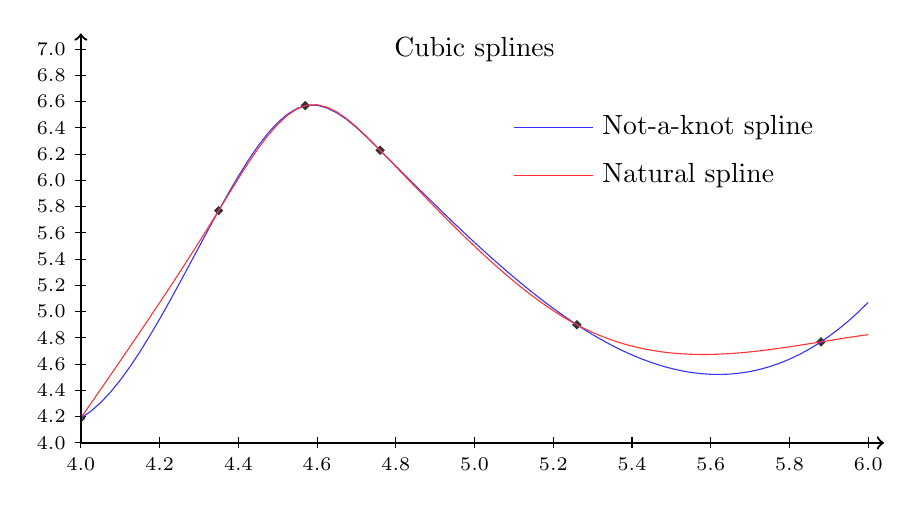
\begin{tikzpicture}
\draw (0.0,0cm + 2pt) -- (0.0, 0cm -2pt) node[below] {\scriptsize{\num[round-mode=places,round-precision=1]{4.0}}};
\draw (0.99999905,0cm + 2pt) -- (0.99999905, 0cm -2pt) node[below] {\scriptsize{\num[round-mode=places,round-precision=1]{4.2}}};
\draw (2.0000005,0cm + 2pt) -- (2.0000005, 0cm -2pt) node[below] {\scriptsize{\num[round-mode=places,round-precision=1]{4.4}}};
\draw (2.9999995,0cm + 2pt) -- (2.9999995, 0cm -2pt) node[below] {\scriptsize{\num[round-mode=places,round-precision=1]{4.6}}};
\draw (4.000001,0cm + 2pt) -- (4.000001, 0cm -2pt) node[below] {\scriptsize{\num[round-mode=places,round-precision=1]{4.8}}};
\draw (5.0,0cm + 2pt) -- (5.0, 0cm -2pt) node[below] {\scriptsize{\num[round-mode=places,round-precision=1]{5.0}}};
\draw (5.999999,0cm + 2pt) -- (5.999999, 0cm -2pt) node[below] {\scriptsize{\num[round-mode=places,round-precision=1]{5.2}}};
\draw (7.0000005,0cm + 2pt) -- (7.0000005, 0cm -2pt) node[below] {\scriptsize{\num[round-mode=places,round-precision=1]{5.4}}};
\draw (7.9999995,0cm + 2pt) -- (7.9999995, 0cm -2pt) node[below] {\scriptsize{\num[round-mode=places,round-precision=1]{5.6}}};
\draw (9.000001,0cm + 2pt) -- (9.000001, 0cm -2pt) node[below] {\scriptsize{\num[round-mode=places,round-precision=1]{5.8}}};
\draw (10.0,0cm + 2pt) -- (10.0, 0cm -2pt) node[below] {\scriptsize{\num[round-mode=places,round-precision=1]{6.0}}};
\draw (0cm + 2pt,0.    ) -- (0cm-2pt,0.    ) node[left] {\scriptsize{\num[round-mode=places,round-precision=1]{4.0}}};
\draw (0cm + 2pt,0.33333302    ) -- (0cm-2pt,0.33333302    ) node[left] {\scriptsize{\num[round-mode=places,round-precision=1]{4.2}}};
\draw (0cm + 2pt,0.6666668    ) -- (0cm-2pt,0.6666668    ) node[left] {\scriptsize{\num[round-mode=places,round-precision=1]{4.4}}};
\draw (0cm + 2pt,0.9999998    ) -- (0cm-2pt,0.9999998    ) node[left] {\scriptsize{\num[round-mode=places,round-precision=1]{4.6}}};
\draw (0cm + 2pt,1.3333336    ) -- (0cm-2pt,1.3333336    ) node[left] {\scriptsize{\num[round-mode=places,round-precision=1]{4.8}}};
\draw (0cm + 2pt,1.6666666    ) -- (0cm-2pt,1.6666666    ) node[left] {\scriptsize{\num[round-mode=places,round-precision=1]{5.0}}};
\draw (0cm + 2pt,1.9999996    ) -- (0cm-2pt,1.9999996    ) node[left] {\scriptsize{\num[round-mode=places,round-precision=1]{5.2}}};
\draw (0cm + 2pt,2.3333335    ) -- (0cm-2pt,2.3333335    ) node[left] {\scriptsize{\num[round-mode=places,round-precision=1]{5.4}}};
\draw (0cm + 2pt,2.6666665    ) -- (0cm-2pt,2.6666665    ) node[left] {\scriptsize{\num[round-mode=places,round-precision=1]{5.6}}};
\draw (0cm + 2pt,3.0000002    ) -- (0cm-2pt,3.0000002    ) node[left] {\scriptsize{\num[round-mode=places,round-precision=1]{5.8}}};
\draw (0cm + 2pt,3.3333333    ) -- (0cm-2pt,3.3333333    ) node[left] {\scriptsize{\num[round-mode=places,round-precision=1]{6.0}}};
\draw (0cm + 2pt,3.6666663    ) -- (0cm-2pt,3.6666663    ) node[left] {\scriptsize{\num[round-mode=places,round-precision=1]{6.2}}};
\draw (0cm + 2pt,4.    ) -- (0cm-2pt,4.    ) node[left] {\scriptsize{\num[round-mode=places,round-precision=1]{6.4}}};
\draw (0cm + 2pt,4.333334    ) -- (0cm-2pt,4.333334    ) node[left] {\scriptsize{\num[round-mode=places,round-precision=1]{6.6000004}}};
\draw (0cm + 2pt,4.666667    ) -- (0cm-2pt,4.666667    ) node[left] {\scriptsize{\num[round-mode=places,round-precision=1]{6.8}}};
\draw (0cm + 2pt,5.    ) -- (0cm-2pt,5.    ) node[left] {\scriptsize{\num[round-mode=places,round-precision=1]{7.0}}};
\node[] at (5.0,5.0) {Cubic splines};
\begin{scope}[]
\clip (0,0) rectangle (10,5);
\node at (0.0,0.316666654083465) [draw=black!80,fill=black!80,diamond,inner sep=0pt,minimum width =3pt,minimum height=3pt] {}; 
\node at (1.7499999739229666,2.949999882777536) [draw=black!80,fill=black!80,diamond,inner sep=0pt,minimum width =3pt,minimum height=3pt] {}; 
\node at (2.8499999575316926,4.283333163128966) [draw=black!80,fill=black!80,diamond,inner sep=0pt,minimum width =3pt,minimum height=3pt] {}; 
\node at (3.799999943375587,3.716666518979609) [draw=black!80,fill=black!80,diamond,inner sep=0pt,minimum width =3pt,minimum height=3pt] {}; 
\node at (6.299999906122685,1.4999999403953581) [draw=black!80,fill=black!80,diamond,inner sep=0pt,minimum width =3pt,minimum height=3pt] {}; 
\node at (9.399999859929085,1.2833332823382497) [draw=black!80,fill=black!80,diamond,inner sep=0pt,minimum width =3pt,minimum height=3pt] {}; 
\begin{scope}[blue!80]
\draw[] (-2.4999999627470975,7.7943914926862305) -- (-2.374999964609743,6.85271188831033);
\draw[] (-2.374999964609743,6.85271188831033) -- (-2.2499999664723886,5.985369091033453);
\draw[] (-2.2499999664723886,5.985369091033453) -- (-2.124999968335032,5.189934920066197);
\draw[] (-2.124999968335032,5.189934920066197) -- (-1.9999999701976776,4.4639811946192065);
\draw[] (-1.9999999701976776,4.4639811946192065) -- (-1.8749999720603232,3.8050797339030833);
\draw[] (-1.8749999720603232,3.8050797339030833) -- (-1.7499999739229688,3.2108023571284394);
\draw[] (-1.7499999739229688,3.2108023571284394) -- (-1.6249999757856144,2.6787208835058913);
\draw[] (-1.6249999757856144,2.6787208835058913) -- (-1.4999999776482578,2.206407132246049);
\draw[] (-1.4999999776482578,2.206407132246049) -- (-1.3749999795109031,1.7914329225595402);
\draw[] (-1.3749999795109031,1.7914329225595402) -- (-1.2499999813735487,1.431370073656974);
\draw[] (-1.2499999813735487,1.431370073656974) -- (-1.1249999832361943,1.1237904047489642);
\draw[] (-1.1249999832361943,1.1237904047489642) -- (-0.9999999850988399,0.8662657350461275);
\draw[] (-0.9999999850988399,0.8662657350461275) -- (-0.8749999869614833,0.6563678837590736);
\draw[] (-0.8749999869614833,0.6563678837590736) -- (-0.7499999888241289,0.49166867009842874);
\draw[] (-0.7499999888241289,0.49166867009842874) -- (-0.6249999906867744,0.36973991327480216);
\draw[] (-0.6249999906867744,0.36973991327480216) -- (-0.49999999254941996,0.2881534324988066);
\draw[] (-0.49999999254941996,0.2881534324988066) -- (-0.3749999944120655,0.24448104698106043);
\draw[] (-0.3749999944120655,0.24448104698106043) -- (-0.24999999627470887,0.23629457593217776);
\draw[] (-0.24999999627470887,0.23629457593217776) -- (-0.12499999813735443,0.26116583856277414);
\draw[] (-0.12499999813735443,0.26116583856277414) -- (0.0,0.316666654083465);
\draw[] (0.0,0.316666654083465) -- (0.12499999813735665,0.4003688417048675);
\draw[] (0.12499999813735665,0.4003688417048675) -- (0.24999999627470887,0.5098442206375896);
\draw[] (0.24999999627470887,0.5098442206375896) -- (0.3749999944120655,0.6426646100922557);
\draw[] (0.3749999944120655,0.6426646100922557) -- (0.49999999254941774,0.7964018292794712);
\draw[] (0.49999999254941774,0.7964018292794712) -- (0.6249999906867744,0.9686276974098632);
\draw[] (0.6249999906867744,0.9686276974098632) -- (0.749999988824131,1.1569140336940429);
\draw[] (0.749999988824131,1.1569140336940429) -- (0.8749999869614833,1.358832657342614);
\draw[] (0.8749999869614833,1.358832657342614) -- (0.9999999850988399,1.5719553875662082);
\draw[] (0.9999999850988399,1.5719553875662082) -- (1.124999983236192,1.793854043575428);
\draw[] (1.124999983236192,1.793854043575428) -- (1.2499999813735487,2.0221004445808974);
\draw[] (1.2499999813735487,2.0221004445808974) -- (1.3749999795109054,2.2542664097932303);
\draw[] (1.3749999795109054,2.2542664097932303) -- (1.4999999776482578,2.487923758423034);
\draw[] (1.4999999776482578,2.487923758423034) -- (1.6249999757856144,2.7206443096809374);
\draw[] (1.6249999757856144,2.7206443096809374) -- (1.7499999739229666,2.9499998827775373);
\draw[] (1.7499999739229666,2.9499998827775373) -- (1.8749999720603232,3.1733231579063315);
\draw[] (1.8749999720603232,3.1733231579063315) -- (1.9999999701976798,3.386990259192244);
\draw[] (1.9999999701976798,3.386990259192244) -- (2.124999968335032,3.5871381717430655);
\draw[] (2.124999968335032,3.5871381717430655) -- (2.2499999664723886,3.7699038806666065);
\draw[] (2.2499999664723886,3.7699038806666065) -- (2.374999964609741,3.931424371070651);
\draw[] (2.374999964609741,3.931424371070651) -- (2.4999999627470975,4.06783662806301);
\draw[] (2.4999999627470975,4.06783662806301) -- (2.624999960884454,4.17527763675147);
\draw[] (2.624999960884454,4.17527763675147) -- (2.7499999590218063,4.24988438224383);
\draw[] (2.7499999590218063,4.24988438224383) -- (2.874999957159163,4.287805970399012);
\draw[] (2.874999957159163,4.287805970399012) -- (2.9999999552965155,4.287761106314666);
\draw[] (2.9999999552965155,4.287761106314666) -- (3.124999953433872,4.254201610371051);
\draw[] (3.124999953433872,4.254201610371051) -- (3.249999951571229,4.192355031020499);
\draw[] (3.249999951571229,4.192355031020499) -- (3.374999949708581,4.1074489167153505);
\draw[] (3.374999949708581,4.1074489167153505) -- (3.4999999478459376,4.004710815907926);
\draw[] (3.4999999478459376,4.004710815907926) -- (3.62499994598329,3.88936827705057);
\draw[] (3.62499994598329,3.88936827705057) -- (3.7499999441206464,3.766648848595603);
\draw[] (3.7499999441206464,3.766648848595603) -- (3.874999942258003,3.641599909911412);
\draw[] (3.874999942258003,3.641599909911412) -- (3.9999999403953552,3.5165729770361955);
\draw[] (3.9999999403953552,3.5165729770361955) -- (4.124999938532712,3.3918442850782133);
\draw[] (4.124999938532712,3.3918442850782133) -- (4.249999936670064,3.2676366857134576);
\draw[] (4.249999936670064,3.2676366857134576) -- (4.374999934807421,3.144173030617912);
\draw[] (4.374999934807421,3.144173030617912) -- (4.499999932944777,3.021676171467562);
\draw[] (4.499999932944777,3.021676171467562) -- (4.6249999310821295,2.9003689599384015);
\draw[] (4.6249999310821295,2.9003689599384015) -- (4.749999929219486,2.7804742477064077);
\draw[] (4.749999929219486,2.7804742477064077) -- (4.874999927356838,2.6622148864475754);
\draw[] (4.874999927356838,2.6622148864475754) -- (4.999999925494195,2.545813727837884);
\draw[] (4.999999925494195,2.545813727837884) -- (5.1249999236315515,2.4314936235533224);
\draw[] (5.1249999236315515,2.4314936235533224) -- (5.249999921768904,2.3194774252698838);
\draw[] (5.249999921768904,2.3194774252698838) -- (5.37499991990626,2.2099879846635475);
\draw[] (5.37499991990626,2.2099879846635475) -- (5.4999999180436125,2.103248153410304);
\draw[] (5.4999999180436125,2.103248153410304) -- (5.624999916180969,1.9994807831861359);
\draw[] (5.624999916180969,1.9994807831861359) -- (5.749999914318326,1.8989087256670316);
\draw[] (5.749999914318326,1.8989087256670316) -- (5.874999912455678,1.8017548325289818);
\draw[] (5.874999912455678,1.8017548325289818) -- (5.999999910593035,1.708241955447969);
\draw[] (5.999999910593035,1.708241955447969) -- (6.124999908730388,1.6185929460999828);
\draw[] (6.124999908730388,1.6185929460999828) -- (6.249999906867744,1.533030656161004);
\draw[] (6.249999906867744,1.533030656161004) -- (6.374999905005101,1.451776384534055);
\draw[] (6.374999905005101,1.451776384534055) -- (6.499999903142453,1.3750281960377477);
\draw[] (6.499999903142453,1.3750281960377477) -- (6.62499990127981,1.3029662698464899);
\draw[] (6.62499990127981,1.3029662698464899) -- (6.749999899417162,1.2357703250538243);
\draw[] (6.749999899417162,1.2357703250538243) -- (6.874999897554519,1.173620080753285);
\draw[] (6.874999897554519,1.173620080753285) -- (6.999999895691875,1.116695256038412);
\draw[] (6.999999895691875,1.116695256038412) -- (7.124999893829227,1.0651755700027439);
\draw[] (7.124999893829227,1.0651755700027439) -- (7.249999891966584,1.0192407417398162);
\draw[] (7.249999891966584,1.0192407417398162) -- (7.374999890103936,0.9790704903431704);
\draw[] (7.374999890103936,0.9790704903431704) -- (7.499999888241293,0.944844534906336);
\draw[] (7.499999888241293,0.944844534906336) -- (7.6249998863786494,0.9167425945228603);
\draw[] (7.6249998863786494,0.9167425945228603) -- (7.749999884516006,0.8949443882862762);
\draw[] (7.749999884516006,0.8949443882862762) -- (7.874999882653358,0.879629635290119);
\draw[] (7.874999882653358,0.879629635290119) -- (7.9999998807907104,0.8709780546279331);
\draw[] (7.9999998807907104,0.8709780546279331) -- (8.124999878928067,0.8691693653932512);
\draw[] (8.124999878928067,0.8691693653932512) -- (8.249999877065424,0.8743832866796089);
\draw[] (8.249999877065424,0.8743832866796089) -- (8.37499987520278,0.8867995375805503);
\draw[] (8.37499987520278,0.8867995375805503) -- (8.499999873340133,0.9065978371896083);
\draw[] (8.499999873340133,0.9065978371896083) -- (8.624999871477485,0.9339579046003212);
\draw[] (8.624999871477485,0.9339579046003212) -- (8.749999869614841,0.9690594589062291);
\draw[] (8.749999869614841,0.9690594589062291) -- (8.874999867752198,1.0120822192008692);
\draw[] (8.874999867752198,1.0120822192008692) -- (8.999999865889555,1.0632059045777764);
\draw[] (8.999999865889555,1.0632059045777764) -- (9.124999864026908,1.12261023413049);
\draw[] (9.124999864026908,1.12261023413049) -- (9.249999862164259,1.190474926952545);
\draw[] (9.249999862164259,1.190474926952545) -- (9.374999860301616,1.2669797021374845);
\draw[] (9.374999860301616,1.2669797021374845) -- (9.499999858438972,1.3523042787788442);
\draw[] (9.499999858438972,1.3523042787788442) -- (9.624999856576329,1.4466283759701621);
\draw[] (9.624999856576329,1.4466283759701621) -- (9.749999854713682,1.5501317128049699);
\draw[] (9.749999854713682,1.5501317128049699) -- (9.874999852851033,1.6629940083768073);
\draw[] (9.874999852851033,1.6629940083768073) -- (9.99999985098839,1.7853949817792232);
\end{scope}
\begin{scope}[red!80]
\draw[] (-2.4999999627470975,-3.605941027545164) -- (-2.374999964609743,-3.38062413015895);
\draw[] (-2.374999964609743,-3.38062413015895) -- (-2.2499999664723886,-3.159797465588856);
\draw[] (-2.2499999664723886,-3.159797465588856) -- (-2.124999968335032,-2.943224705791926);
\draw[] (-2.124999968335032,-2.943224705791926) -- (-1.9999999701976776,-2.730669522725212);
\draw[] (-1.9999999701976776,-2.730669522725212) -- (-1.8749999720603232,-2.5218955883457586);
\draw[] (-1.8749999720603232,-2.5218955883457586) -- (-1.7499999739229688,-2.3166665746106103);
\draw[] (-1.7499999739229688,-2.3166665746106103) -- (-1.6249999757856144,-2.114746153476813);
\draw[] (-1.6249999757856144,-2.114746153476813) -- (-1.4999999776482578,-1.9158979969014112);
\draw[] (-1.4999999776482578,-1.9158979969014112) -- (-1.3749999795109031,-1.7198857768414577);
\draw[] (-1.3749999795109031,-1.7198857768414577) -- (-1.2499999813735487,-1.526473165253995);
\draw[] (-1.2499999813735487,-1.526473165253995) -- (-1.1249999832361943,-1.3354238340960685);
\draw[] (-1.1249999832361943,-1.3354238340960685) -- (-0.9999999850988399,-1.1465014553247257);
\draw[] (-0.9999999850988399,-1.1465014553247257) -- (-0.8749999869614833,-0.95946970089701);
\draw[] (-0.8749999869614833,-0.95946970089701) -- (-0.7499999888241289,-0.7740922427699727);
\draw[] (-0.7499999888241289,-0.7740922427699727) -- (-0.6249999906867744,-0.5901327529006577);
\draw[] (-0.6249999906867744,-0.5901327529006577) -- (-0.49999999254941996,-0.4073549032461111);
\draw[] (-0.49999999254941996,-0.4073549032461111) -- (-0.3749999944120655,-0.2255223657633807);
\draw[] (-0.3749999944120655,-0.2255223657633807) -- (-0.24999999627470887,-0.04439881240950658);
\draw[] (-0.24999999627470887,-0.04439881240950658) -- (-0.12499999813735443,0.1362520848584554);
\draw[] (-0.12499999813735443,0.1362520848584554) -- (0.0,0.316666654083465);
\draw[] (0.0,0.316666654083465) -- (0.12499999813735665,0.4970812233084776);
\draw[] (0.12499999813735665,0.4970812233084776) -- (0.24999999627470887,0.677732120576436);
\draw[] (0.24999999627470887,0.677732120576436) -- (0.3749999944120655,0.8588556739303093);
\draw[] (0.3749999944120655,0.8588556739303093) -- (0.49999999254941774,1.040688211413039);
\draw[] (0.49999999254941774,1.040688211413039) -- (0.6249999906867744,1.2234660610675885);
\draw[] (0.6249999906867744,1.2234660610675885) -- (0.749999988824131,1.4074255509369065);
\draw[] (0.749999988824131,1.4074255509369065) -- (0.8749999869614833,1.5928030090639387);
\draw[] (0.8749999869614833,1.5928030090639387) -- (0.9999999850988399,1.7798347634916558);
\draw[] (0.9999999850988399,1.7798347634916558) -- (1.124999983236192,1.9687571422629948);
\draw[] (1.124999983236192,1.9687571422629948) -- (1.2499999813735487,2.159806473420925);
\draw[] (1.2499999813735487,2.159806473420925) -- (1.3749999795109054,2.353219085008392);
\draw[] (1.3749999795109054,2.353219085008392) -- (1.4999999776482578,2.5492313050683406);
\draw[] (1.4999999776482578,2.5492313050683406) -- (1.6249999757856144,2.748079461643744);
\draw[] (1.6249999757856144,2.748079461643744) -- (1.7499999739229666,2.9499998827775373);
\draw[] (1.7499999739229666,2.9499998827775373) -- (1.8749999720603232,3.154329772046608);
\draw[] (1.8749999720603232,3.154329772046608) -- (1.9999999701976798,3.356809835163513);
\draw[] (1.9999999701976798,3.356809835163513) -- (2.124999968335032,3.552281653374717);
\draw[] (2.124999968335032,3.552281653374717) -- (2.2499999664723886,3.735586807926718);
\draw[] (2.2499999664723886,3.735586807926718) -- (2.374999964609741,3.9015668800659786);
\draw[] (2.374999964609741,3.9015668800659786) -- (2.4999999627470975,4.045063451038991);
\draw[] (2.4999999627470975,4.045063451038991) -- (2.624999960884454,4.160918102092223);
\draw[] (2.624999960884454,4.160918102092223) -- (2.7499999590218063,4.243972414472157);
\draw[] (2.7499999590218063,4.243972414472157) -- (2.874999957159163,4.289082111375187);
\draw[] (2.874999957159163,4.289082111375187) -- (2.9999999552965155,4.294101009379233);
\draw[] (2.9999999552965155,4.294101009379233) -- (3.124999953433872,4.263572067371012);
\draw[] (3.124999953433872,4.263572067371012) -- (3.249999951571229,4.202943329031665);
\draw[] (3.249999951571229,4.202943329031665) -- (3.374999949708581,4.117662838042336);
\draw[] (3.374999949708581,4.117662838042336) -- (3.4999999478459376,4.01317863808416);
\draw[] (3.4999999478459376,4.01317863808416) -- (3.62499994598329,3.8949387728382847);
\draw[] (3.62499994598329,3.8949387728382847) -- (3.7499999441206464,3.768391285985844);
\draw[] (3.7499999441206464,3.768391285985844) -- (3.874999942258003,3.6388018959505035);
\draw[] (3.874999942258003,3.6388018959505035) -- (3.9999999403953552,3.5087081950810326);
\draw[] (3.9999999403953552,3.5087081950810326) -- (4.124999938532712,3.3785476588715095);
\draw[] (4.124999938532712,3.3785476588715095) -- (4.249999936670064,3.248703740517511);
\draw[] (4.249999936670064,3.248703740517511) -- (4.374999934807421,3.1195598932146047);
\draw[] (4.374999934807421,3.1195598932146047) -- (4.499999932944777,2.9914995701583624);
\draw[] (4.499999932944777,2.9914995701583624) -- (4.6249999310821295,2.864906224544363);
\draw[] (4.6249999310821295,2.864906224544363) -- (4.749999929219486,2.740163309568167);
\draw[] (4.749999929219486,2.740163309568167) -- (4.874999927356838,2.617654278425355);
\draw[] (4.874999927356838,2.617654278425355) -- (4.999999925494195,2.497762584311492);
\draw[] (4.999999925494195,2.497762584311492) -- (5.1249999236315515,2.380871680422152);
\draw[] (5.1249999236315515,2.380871680422152) -- (5.249999921768904,2.267365019952912);
\draw[] (5.249999921768904,2.267365019952912) -- (5.37499991990626,2.157626056099335);
\draw[] (5.37499991990626,2.157626056099335) -- (5.4999999180436125,2.0520382420570016);
\draw[] (5.4999999180436125,2.0520382420570016) -- (5.624999916180969,1.9509850310214718);
\draw[] (5.624999916180969,1.9509850310214718) -- (5.749999914318326,1.8548498761883265);
\draw[] (5.749999914318326,1.8548498761883265) -- (5.874999912455678,1.764016230753138);
\draw[] (5.874999912455678,1.764016230753138) -- (5.999999910593035,1.6788675479114719);
\draw[] (5.999999910593035,1.6788675479114719) -- (6.124999908730388,1.5997872808589044);
\draw[] (6.124999908730388,1.5997872808589044) -- (6.249999906867744,1.5271588827910019);
\draw[] (6.249999906867744,1.5271588827910019) -- (6.374999905005101,1.4613418576961836);
\draw[] (6.374999905005101,1.4613418576961836) -- (6.499999903142453,1.4023373584631706);
\draw[] (6.499999903142453,1.4023373584631706) -- (6.62499990127981,1.3498706785945276);
\draw[] (6.62499990127981,1.3498706785945276) -- (6.749999899417162,1.3036600155314544);
\draw[] (6.749999899417162,1.3036600155314544) -- (6.874999897554519,1.2634235667151321);
\draw[] (6.874999897554519,1.2634235667151321) -- (6.999999895691875,1.2288795295867583);
\draw[] (6.999999895691875,1.2288795295867583) -- (7.124999893829227,1.1997461015875226);
\draw[] (7.124999893829227,1.1997461015875226) -- (7.249999891966584,1.175741480158612);
\draw[] (7.249999891966584,1.175741480158612) -- (7.374999890103936,1.1565838627412233);
\draw[] (7.374999890103936,1.1565838627412233) -- (7.499999888241293,1.1419914467765409);
\draw[] (7.499999888241293,1.1419914467765409) -- (7.6249998863786494,1.1316824297057606);
\draw[] (7.6249998863786494,1.1316824297057606) -- (7.749999884516006,1.1253750089700705);
\draw[] (7.749999884516006,1.1253750089700705) -- (7.874999882653358,1.1227873820106633);
\draw[] (7.874999882653358,1.1227873820106633) -- (7.9999998807907104,1.1236377462687277);
\draw[] (7.9999998807907104,1.1236377462687277) -- (8.124999878928067,1.127644299185455);
\draw[] (8.124999878928067,1.127644299185455) -- (8.249999877065424,1.1345252382020363);
\draw[] (8.249999877065424,1.1345252382020363) -- (8.37499987520278,1.143998760759663);
\draw[] (8.37499987520278,1.143998760759663) -- (8.499999873340133,1.155783064299525);
\draw[] (8.499999873340133,1.155783064299525) -- (8.624999871477485,1.1695963462628136);
\draw[] (8.624999871477485,1.1695963462628136) -- (8.749999869614841,1.1851568040907217);
\draw[] (8.749999869614841,1.1851568040907217) -- (8.874999867752198,1.2021826352244345);
\draw[] (8.874999867752198,1.2021826352244345) -- (8.999999865889555,1.220392037105148);
\draw[] (8.999999865889555,1.220392037105148) -- (9.124999864026908,1.2395032071740488);
\draw[] (9.124999864026908,1.2395032071740488) -- (9.249999862164259,1.2592343428723314);
\draw[] (9.249999862164259,1.2592343428723314) -- (9.374999860301616,1.2793036416411872);
\draw[] (9.374999860301616,1.2793036416411872) -- (9.499999858438972,1.2994293009218014);
\draw[] (9.499999858438972,1.2994293009218014) -- (9.624999856576329,1.3193295181553697);
\draw[] (9.624999856576329,1.3193295181553697) -- (9.749999854713682,1.3387224907830808);
\draw[] (9.749999854713682,1.3387224907830808) -- (9.874999852851033,1.3573264162461258);
\draw[] (9.874999852851033,1.3573264162461258) -- (9.99999985098839,1.3748594919856976);
\end{scope}
\end{scope}
\draw[blue!80] (5.5,4.0) -- (6.5,4.0);
\node[right,] at (6.5,4.0) {Not-a-knot spline};
\draw[red!80] (5.5,3.4) -- (6.5,3.4);
\node[right,] at (6.5,3.4) {Natural spline};
\draw[thick,->] (0.0,0.0) -- (10.2,0.0);
\draw[thick,->] (0.0,0.0) -- (0.0,5.2);
\end{tikzpicture}
%%% Local Variables: 
%%% mode: latex 
%%% TeX-master: "master" 
%%% End:



\end{document}


  
%%% Local Variables: 
%%% mode: latex
%%% TeX-master: t
%%% End: 
